%
% skript.tex -- Lecture notes for the PartDiff lectures given at the
%               MSE Master
%
% (c) 2006-2018 Prof. Dr. Andreas Mueller, HSR
%
\documentclass[a4paper,12pt]{book}
\usepackage[utf8]{inputenc}
\usepackage[T1]{fontenc}
%\usepackage{german}
\usepackage{times}
\usepackage{geometry}
\geometry{papersize={210mm,297mm},total={160mm,240mm},top=31mm,bindingoffset=15mm}
\usepackage{amsmath}
\usepackage{amssymb}
\usepackage{amsfonts}
\usepackage{amsthm}
\usepackage{amscd}
\usepackage{graphicx}
\usepackage{fancyhdr}
\usepackage{textcomp}
\usepackage{txfonts}
\usepackage[all]{xy}
\usepackage{paralist}
\usepackage[colorlinks=true]{hyperref}
\usepackage{array}
\usepackage{tikz}
\input{../common/linsys.tex}
\makeindex
\begin{document}
\pagestyle{fancy}
\lhead{}
\rhead{}
\frontmatter
\newcommand\HRule{\noindent\rule{\linewidth}{1.5pt}}
\begin{titlepage}
\vspace*{\stretch{1}}
\HRule
\vspace*{10pt}
\begin{flushright}
{\Huge
Partial Differential Equations}
\end{flushright}
\begin{flushright}
{\Large Part 1: General Theory}
\end{flushright}
\HRule
\begin{flushright}
\vspace{30pt}
\LARGE
Andreas Müller
\end{flushright}
\vspace*{\stretch{2}}
\begin{center}
Hochschule für Technik, Rapperswil, 2008-2019
\end{center}
\end{titlepage}
\hypersetup{
    colorlinks=true,
    linktoc=all,
    linkcolor=blue
}
\tableofcontents
\newtheorem{satz}{Theorem}[chapter]
\newtheorem{problem}[satz]{Problem}
\newtheorem{hilfssatz}[satz]{Lemma}
\newtheorem{definition}[satz]{Definition}
\newtheorem{annahme}[satz]{Assumption}
\newtheorem{aufgabe}[satz]{Task}
\newenvironment{beispiel}[1][Example]{%
\begin{proof}[#1]%
\renewcommand{\qedsymbol}{$\bigcirc$}
}{\end{proof}}
\mainmatter
%
% a-einleitung.tex
%
% (c) 2008 Prof Dr Andreas Mueller, Hochschule Rapperswil
%
\lhead{Introduction}
\chapter*{Introduction}
\index{mechanics!classical}
\index{electrodynamics}
\index{population dynamics}
Ordinary differential equations are used in classical mechanics,
in electrodynamics, in population dynamics and more generally in any
application where the rate of change of a variable depends on the current
values of the same variable.
\index{point mass}
\index{Newton's law}
A point mass at coordinate $x$ changes its position according to 
Newton's law
\[
ma=m\ddot x=F.
\]
If the force $F$ depends on the position of the mass, as e.~g.~in the
case of a weight suspended from a spring, we get a differential equation
for the time dependent position $x(t)$:
\[
m\frac{d^2}{dt^2}x(t)=F(x(t)).
\]
Classical analysis proves theorems that show that we can expect such
a differential equation to have a unique solution for each
initial condition under relatively mild assumptions on the function $F$.
Only slight additional work is required for differential equations 
for a vector valued function.

\index{fields!electrical}
\index{temperature distribution}
\index{pressure}
\index{gas}
\index{flow}
\index{fluid}
To describe electrical fields, temperature distributions, pressure
in a gas or flow velocity in a fluid, we need to determine functions 
that do not only depend on a single time variable, but also on additional
variables like position and velocity.
In addition, the rate of change over time of these quantities may also depend
on the rate of change with respect to spacial displacements.

The deflection of a vibrating string is a function $f(x,t)$, where $x$ is
the position along the string and $t$ is time.
\index{string}
For each point $t_0$ in time, the shape of the string is different and
described by the function $x\mapsto f(x,t_0)$.
Any hope that it might be possible to derive a differential equation
for the motion of point on the string in isolation is quickly dashed
by the simple observation, that the force acting on such point
increases if neightboring points are deviate more from a straight line.
This means that the acceleration of a point on the string depends on 
the curvature.
We therefore expect an equation that links the second time derivative of $f$
to the second spacial derivative.
The equation we will later derive is the wave equation, it has the form
\index{wave equation}
\begin{align*}
a^2\frac{\partial^2}{\partial x^2}f&= \frac{\partial^2}{\partial t^2}f.
\end{align*}
If we are able to solve such a partial differential equation,
we will be able to predict the shape of the string for every point in
time.
Equivalently, we will be able to predict the movement $t\mapsto f(x_0,t)$
for every point $x_0$ on the string.
\index{differential equation!partial}

\index{Differentialgleichung!gew\"ohnliche}
The theory of ordinary differential equations shows that the equation
by itself does not determine the solution.
Additional data in the form of initial or boundary conditions has to be
specified.
Partial differential equations will not be different in that regard.
The theory thus has to provide answers to the following questions:
\begin{enumerate}
\item
How do we have to formulate the differential equation in order to ensure
that a solution will be well defined?
\item
What properties will the solution have?
What does the solution look like close to the boundary, does it remain
continuous or differentiable, does it increase beyond any limit?
\item
How can we compute solutions numerically?
\end{enumerate}
This course tries to give some basics answers to these questions.
It has two parts.
The first part deals with the theoretical basics.
It teaches how to set up a problem involving partial differential equations
so that conclusions about existence and uniqueness of solutions are possible.
In some cases, we will even be able to find a solution in closed form.
This, however, will be rather the exception than the rule.
The second part then strives to actually compute these solutions using
a computer algorithm.

The present lecture notes cover the first part of the course.
They are structured as follows:
\begin{enumerate}
\item
Examples of partial differential equations.
The most important partial differential equations from mechanics,
thermodynamics and electrodynamics are presented.
They serve as prototypical examples in later chapters to illustrate
and apply the theoretical insights.
\item
Method of separation of variables.
\item
Solutions using integral transforms like the Laplace transform or the 
Fourier transform.
\index{Laplace transform}
\index{Fourier transform}
\item
Classification of partial differential equations of second order.
These equations turn out to be of utmost practical importance, but
they arise in three distinctly different types with very different properties
and which require vastly different solution methods.
\item
Elliptic partial differential equations.
\item
Parabolic partial differential equations with the heat equation as the
prime example.
\index{parabolic}
\index{heat equation}
\item
Hyperbolic partial differential equations with the wave equation as the
prime example.
\index{hyperbolic}
\index{wave equation}
\item
Some nonlinear partial differential equations.
\end{enumerate}



%
% examples.tex
%
% (c) 2019 Prof Dr Andreas Mueller
%
\chapter{Introductory examples of partial differential equations
\label{chapter:examples}}
\lhead{Introductory examples}
In this chapter we present a few partial differential equations
of prime practical importance which will also serve us as case
studies to illustrate general theorems and solution techniques.
The examples illustrate
\begin{enumerate}
\item
the manifold applications of the theory of partial differential equations,
\item
three completely different cases that lead to incompatible solution
algorithms and
\item
the importance of boundary and initial conditions.
\end{enumerate}

%
% waveequation.tex -- the wave equation
%
% (c) 2019 Prof Dr Andreas Mueller
%
\rhead{Wave equation}
\section{Wave equation\label{beispiele:wellengleichung}}
\index{wave equation}
In the simplest form, this equation describes the motion
of a string of a guitar or a piano, or the air column of a 
wind instrument.
It can be generalized to vibration of a membrane or the fluid inside
an arbitrary threedimensional volume.
Electromagnetic waves can be modelled with this equation just as
well as the waves on the surface of a lake.

\subsection{The differential equation of a vibrating string}
\index{string}
Let a thin string with linear mass density $\mu$ be mounted between
the points $x=0$ and $x=l$.
The force $F$ at the end points of the string maintains its tension.
We ask for a partial differential that describes the motion of a
string after we bring it into a certain shape and let it go at time $t=0$

The state of the string at any time can be described by a function
$u(x,t)$, which measures the deflection of the string from the straight
line between the two end points.
We need to find a differential equation for the function $u$.

From this problem description we can already derive some information
about the solution.
We note that the end points of the string are fixed, so
\[
u(0,t)=u(l,t)=0\quad\forall t\ge 0.
\]
We call this a boundary condition.
At time $t=0$ the string is supposed to have a given shape.
This is the situation of the guitar player who plucks a string and then
lets it go.
Mathematically we can formulate this as the initial condition
\[
u(x,t) = f(x)\qquad 0 < x < l.
\]
A piano however works differently, at $t=0$ it imparts a certain velocity
profile on the string, or in mathematical form
\[
\frac{partial}{\partial t}u(0,x) = g(x),\qquad 0<x<l.
\]

\begin{figure}
\begin{center}
\includegraphics[width=\hsize]{../common/images/saite-1}
\end{center}
\caption{Derivation of the differential equation of a vibrating string
\label{saite}}
\end{figure}
To derive the equation of motion of a vibrating string, we consider
a small section of the string between coordinates $x$ and $x+\Delta x$
(figure \ref{saite}).
Newton's law says that the acceleration of this piece of string 
is proportional to forces acting on it, with the mass as proportionality
factor.
The mass of this piece of the string is $m=\mu\Delta x$.
At each end of the segment, a force of absolute value $F$ pulls the piece
outward, but these forces don't necessarily have the same direction,
resulting in a vertical force component.
This component turns out to be
\[
F\frac{\partial u}{\partial x}(x+\Delta x)-F\frac{\partial u}{\partial x}(x).
\]
Since the acceleration of the string segment is
$\frac{\partial^2u}{\partial t^2}$
we obtain the equation of motion
\begin{align*}
\mu\Delta x\frac{\partial^2u}{\partial t^2}(x)&=
F\frac{\partial u}{\partial x}(x+\Delta x)-F\frac{\partial u}{\partial x}(x)\\
\Rightarrow\qquad
\frac{\mu}{F}\frac{\partial^2u}{\partial t^2}(x)&=
\frac1{\Delta x}\left(\frac{\partial u}{\partial x}(x+\Delta x)-\frac{\partial u}{\partial x}(x)\right)
\end{align*}
By going to the limit 
$\Delta x\to 0$ we obtain the partial differential equation
\[
\frac{\partial^2u}{\partial t^2}=\frac{F}{\mu}\frac{\partial^2u}{\partial x^2}.
\]
The coefficient
$\frac{F}{\mu}$
has the dimension of a velocity squared, it is the velocity by which waves
propagate along the string.

\subsection{The differential equation of an organ pipe}
The analysis of the vibrating string carries over almost unchanged
to a pipe organ (or any other wind instrument).
The deflection of the string is replaced by a deviation of the pressure.
We then obtain the wave equation
\[
\frac{\partial^2p}{\partial t^2}=
a^2\frac{\partial^2p}{\partial x^2}
\]
Again, $a$ is the speed of sound.

The boundary conditions, however, turn out to be more complicated and more
interesting.
If the end of the pipe is closed, then the air cannot move at this end.
Because movement of the air in the pipe is always associated with pressure
differences, we conclude that there cannot be a pressure gradient at the
end of the pipe in this case.
This leads to the so called Neumann boundary condition
\[
\frac{\partial}{\partial x}p(x_0,t) = 0\qquad t>0.
\]
If the pipe is open, then there is nothing that keeps the air in the pipe,
air can move freely, and the pressure is always as the surrounding air.
This leads to the so called Dirichlet boundary condition
\[
u(x_0,t)=0\qquad t>0.
\]

\subsection{Wave equation in two and three dimensions}
In analogy with the differential equation of a string we can derive the
equation of motion of a membrane fixed around its perimeter.
Let $G$ be a domain in $\mathbb R^2$, and let $\gamma\subset G$ be
the boundary curve of the domain, i.~e.~$\gamma = \partial G$.
Then the deviation of the membrane from zero position is a function
\[
 u \colon G\times \mathbb R_{t \ge 0}\to\mathbb R\colon (x,y,t)\mapsto  u (x,y,t)
\]
The membrane is fixed at the boundary, so $u$ has to satisfy the
boundary conditions
\[
 u (x,y,t)=0\qquad \forall (x,y)\in\gamma,\quad t\ge 0.
\]
The function satisfies the differential equation
\[
\frac{\partial^2 u }{\partial t^2}
=
c^2\left(\frac{\partial^2 u }{\partial x^2}
+
\frac{\partial^2 u }{\partial y^2}\right).
\]
The solution is only determined, if we know the initial shape of the
membrane and its velocity. 
This leads to the initial conditions
\[
 u (x,y,0)=f(x,y)\qquad \forall (x,y)\in G.
\]

In three dimensions, the wave equation becomes
\[
\frac{\partial^2 u }{\partial t^2}
=c^2\left(\frac{\partial^2 u }{\partial x^2}
+\frac{\partial^2 u }{\partial y^2}
+\frac{\partial^2 u }{\partial z^2}
\right).
\]
The additional data required also becomes a bit more involved.
First we have to define a domain 
$G\subset \mathbb R^3$ in threedimensional space.
The boundary of this volume must be a sufficiently smooth surface.
The solution then has to satisfy the boundary conditions
$u(x,y,z,t) = 0$ for points
$(x,y,z)\in \partial G$ on the boundary surface of $G$.

\subsection{The Laplace operator\label{beispiele:laplaceoperator}}
In all the problems discussed so far, the Laplace operator,
also called laplacian,
\[
\Delta
=
\begin{cases}
\displaystyle
\frac{\partial^2}{\partial x^2}
+\frac{\partial^2}{\partial y^2}&\qquad\text{2 Dimensionen}\\
\\
\displaystyle
\frac{\partial^2}{\partial x^2}
+\frac{\partial^2}{\partial y^2}
+\frac{\partial^2}{\partial z^2}&\qquad\text{3 Dimensionen}
\end{cases}
\]
appeared.
In fact, up to a constant factor, this is the only linear operator involving
only second derivatives that is invariant with arbitrary rotations of the
coordinate system.
This means that this is the only operator that can have a physical
meaning independent of the choice of coordinate system.


%
% poissonproblem.tex
%
% (c) 2019 Prof Dr Andreas Mueller
%
\section{Poisson problem}
\rhead{Poisson problem}
\label{poisson-problem}
This section describes two examples of elliptic partial differential
equations, to be expanded on in chapter~\ref{chapter-elliptisch}.

\subsection{Minimal surfaces\label{beispiele:minimal surfaces}}
What shape will a soap film take when it is lifted to height
$f(x,y)$ at the boundary $(x,y)\in\gamma$ of 
a two dimensional domain $G\subset \mathbb R^2$?
If we describe the height of the soap film using a function
$u(x,y)$, we expect to find a partial differential equation for $u$
with boundary condition $f$.
\index{minimal surface}

In the derivation of the equation of motion for the vibrating string
we learned that the force accelerating the string depended on the
curvature of the string.
For the soap film, the restoring force is provided by the surface
tension which is equally strong in each direction of the film.
The soap film has two directions in which it can curve, roughly
given by the second partial derivatives $\partial^2 u/\partial x^2$ and
$\partial^2 u/\partial y^2$.
We therefore expect that force accelerating the film proportional
to the sum of these second derivatives with respect to $x$ and $y$.
Since the film is supposed not to move, we expect the differential
equation:
\[
\frac{\partial^2 u }{\partial x^2}+\frac{\partial^2 u }{\partial y^2}
=\Delta u =0.
\]

This simplified derivation is only valid for small deviations.
More generally, the so called mean curvature of the surface needs
to vanish for a minimal surface.
\index{mean curvature}

\subsection{Electric potential}
\index{electric potential}
In electrodynamics it is shown that a static electric field is a 
gradient field, i.~e.~there is a potential $\varphi$ such that the
electric field
\[
\vec E=\operatorname{grad}\varphi
\]
is its gradient.
It is also shown that the sources of the field are the electric charges.
Without charges, there are no sources to the field.
The mathematical expression of these facts is that 
the electric field satisfies the same partial differential equation
\[
\operatorname{div}\vec E=\operatorname{div}\operatorname{grad}\varphi
=\Delta \varphi=0
\]
as a minimal surface.
This problem seems to have mathematical significance independent of the
particular application.


%
% heatequation.tex -- heat equation
%
% (c) 2008 Prof Dr Andreas Mueller
%
\rhead{Heat equation}
\section{Heat equation}
\index{heat equation}
The heat equation is a prototype for a so called parabolic differential
equation.
\index{parabolic}
Such equations are also used to describe diffusion processes.
The Schrödinger equation, the basis of quantum mechanics, is also of this type.
\index{Schrödinger equation}
\index{quantum mechanics}

We derive the heat equation for the one dimensional case.
We examine a rod of length $l$ between $x$-coordinates $0$ and $l$
and strive to compute the temperature distribution $T(x,t)$ for 
$0<x<l$ and for all times $t>0$.
We need the initial temperature distribution, which we call
$T(x,0) = f(x)$.
We expect to solve this problem using a partial differential equation.

The heat that flows in a time interval $\Delta t$ through the rod at
coordinate $x$ is proportional to the temperature gradient at that point.
The amount of heat flowing into the section  of the rod between
$x$ and $x+\Delta x$ is therefore proportional to
\[
\underbrace{
\frac{\partial T}{\partial x}(x+\Delta x)}
_{\parbox{4cm}{\raggedright\centering heat flow into segment through $x+\Delta x$}}
-
\underbrace{\frac{\partial T}{\partial x}(x).}_{\parbox{3.2cm}{\raggedright
\centering
heat flow out of segment through $x$}}
\]
This additional heat lets the temperature of the segment rise, depending
on the heat capacity of the material.
The volume of the segment is $\Delta x$, the temperature change is smaller
when the volume is larger.
It becomes
\[
\Delta T
=
\kappa
\frac{1}{\Delta x}
\biggl(
\frac{\partial T}{\partial x}(x+\Delta x)-\frac{\partial T}{\partial x}(x).
\biggr) \Delta t,
\]
Where $\kappa$ combines the various physical constants involved into
a single proportionality factor.
Dividing by $\Delta t$ and going to the limits $\Delta t\to 0$
and $\Delta x\to 0$ leads to
\begin{equation}
\lim_{\Delta t\to 0}\frac{\Delta T}{\Delta t}
=
\frac{\partial T}{\partial t}
=
\kappa
\lim_{\Delta x\to 0}\frac1{\Delta x}\left(\frac{\partial T}{\partial x}(x+\Delta x)-\frac{\partial T}{\partial x}(x)\right)
=\kappa\frac{\partial^2T}{\partial x^2}.
\label{examples:heat-equation}
\end{equation}

Again we have to specify suitable initial and boundary conditions.
As initial condition we already have found
\[
T(x,0)=f(x)\qquad \forall x\in[0,l].
\]
As a boundary condition at the end of the rod we could prescribe the
temperature.
In physics terms this means that both ends of the rod are in contact
with a heat reservoir at constant temperature.
If we prescribe the derivatives of $T$ with respect to $x$ at $x=0$ and
$x=l$, we fix the flow of heat into the rod.
In particular, requiring
\[
\frac{\partial T}{\partial x} = 0
\]
means that no heat flows through the ends of the rod, the rod is
thermally isolated from its environment.

A particularly interesting case arises when we ask for a stationary
temperature distribution.
This is the equilibrium distribution a system reaches after sufficiently
long time.
Since in this case the partial derivative with respect to time 
vanishes, the temperature distribution satisfies
$\Delta T=0$, so we are back to the Poisson problem.

So far, we have not considered heat sources in the interior.
This situation models what happens inside the food in a microwave oven: the
microwave radiation is absorbed by the food and heats it up locally.
This can be modelled by adding an additional term on the right hand
side of the heat equation \eqref{examples:heat-equation}.
For the stationary distribution, we are back to the inhomgeneous Poisson
problem.




%
% supersonic.tex -- the equation for a supersonic flow
%
% (c) 2008 Prof Dr Andreas Mueller
%
\rhead{Supersonic flow}
\section{Supersonic flow}
In the year 1928, Jakob Ackeret habilitated at ETH Zürich with a 
\index{Ackeret, Jakob}
\index{supersonic flow}
paper with the title
``Über Luft-Kräfte bei sehr grossen
Geschwindigkeiten insbesondere bei ebenen Strömungen''.
He showed how to compute the aerodynamic forces on an object
in a supersonic flow using a linear approximation.
The velocity field of the gas that enters the region of interest with
velocity $v_1$ in $x$-direction turns out to be the gradient of
a function $\varphi(x,y,z)$ that satisfies the equation
\[
(1-\textit{Ma}_1)\frac{\partial^2\varphi}{\partial x^2}
+
\frac{\partial^2\varphi}{\partial y^2}
+
\frac{\partial^2\varphi}{\partial z^2}=0.
\]
The expression
$\textit{Ma}_1=\frac{v_1}{c_1}$ is called the Mach number of the flow,
$c_1$ is the speed of sound.
The Mach number expresses the flow velocity in units of the speed of sound.

For small velocities, we have $(1-\textit{Ma}_1)>0$, and the equation
becomes similar to the Poisson problem.
This is called potential flow.

\begin{figure}
\begin{center}
\includegraphics[width=0.8\hsize]{../common/graphics/i-5-1}
\end{center}
\caption{Flow around a supersonic plane\label{examples:ueberschall2d}}
\end{figure}

For supersonic flow, however, the first term
$(1-\textit{Ma}_1) < 0$
changes sign, and the equation behaves like a wave equation.
In fact, the flow shows shock waves propagating away from the object
and thus carrying away its energy
(figure~\ref{examples:ueberschall2d}).
By carefully analyzing this solution, Ackeret was able to compute
aerodynamic drag due to these shock waves.
\index{areodynamic drag}
\index{shock waves}


%
% beamequation.tex -- beam equation
%
% (c) 2019 Prof Dr Andreas Mueller
%
\rhead{Beam equation}
\section{Beam equation}
In the derivation of the differential equation of a string we
have used that fact that the string does not resist to being
bent.
Even large curvature of the string does not result in force trying
to straighten it out again.
A beam behaves completely differently.
Bending the beam creates internal stresses in the beam that
try to bring the beam back to its original shape.
We don't try to explain these forces, but it is natural to expect that
they will be proportional to the curvature and thus to the second
derivatives of the beam.
In addition, the are proportional to some material constants
(the elastic modulus $E$)
and to a property derived from the cross section of the beam,
namely the second moment $I$%
\footnote{The definition of $I$ is not relevant for the present
discussion.}.

A segment of length $\Delta x$ of a beam with linear mass density $m$
therefore experiences the following force components:
\begin{enumerate}
\item
Restoring forces caused by the stresses in the beam:
$-EI\frac{\partial^4}{\partial^4 x}w(t,x)\Delta x$
\item
Damping
$-b\frac{\partial}{\partial t}w(t,x)\Delta x$
\item
Exterior forces, e.~g.~loads on the beam:
$q(x,t)\Delta x$
\end{enumerate}
By Newton's law, these forces musst sum up to
\[
m\Delta x\frac{\partial^2}{\partial^2 t}w(t,x).
\]
By going to the limit $\Delta x\to 0$ once more we get
\begin{align*}
m\frac{\partial^2}{\partial^2t}w(t,x)
&=-EI\frac{\partial^4}{\partial^4x}w(t,x)-b\frac{\partial}{\partial t}w(t,x)+q(t,x)
\\
EI\frac{\partial^4}{\partial^4x}w(t,x)
+b\frac{\partial}{\partial t}w(t,x)
+m\frac{\partial^2}{\partial^2t}w(t,x)
&=q(t,x)
\end{align*}
The motion of a beam therefore follows a partial differential equation.


%
% plateequation.tex -- the plate equation
%
% (c) 2019 Prof Dr Andreas Mueller
%
\rhead{Plate equation}
\section{Plate equation}
Still a bit more complicated is the equation of motion for a plate.
\index{plate}
Again, a plate is different from a membrane in that it resists bending
even if not under tension.
If $w(x,y)$ is the deviation of a plate from its shape at point $(x,y)$,
we get the differential equation
\[
D\left(
\frac{\partial^2}{\partial^2 x}
+
\frac{\partial^2}{\partial^2 y}
\right)
\left(
\frac{\partial^2}{\partial^2 x}
+
\frac{\partial^2}{\partial^2 y}
\right)
w(x,y)
=D\Delta\Delta w(x,y)
=p(x,y)
\]
for the static deformation of the plate under load.
$D$ is again some material constant and $p(x,y)$ is the pressure at
$(x,y)$ on the plate.
\index{pressure}
The double Laplacian $\Delta\Delta$ is not a typo, the plate equation
is a fourth order partial differential equation just like the beam
equation~\eqref{examples:beam-equation}.




\section{Summary\label{examples:summary}}
\begin{enumerate}
\item 
Partial differential equations appear in physics whenever fields need
to be described: waves, pressure, temperature, velocity, potential,
electric field,\dots
\item
The Laplace-Operator seems to be ubiquitous in these equations.
\end{enumerate}

%
% classification.tex
% 
% (c) 2019 Prof Dr Andreas Mueller
%
\chapter{Terminology and Notation
\label{chapter:terminology-and-notation}}
\lhead{Terminology and notation}
Partial differential equations are equations for an unknown function of
several variables, linking values of the function to its partial
derivatives.
In this chapter, we write the unknown function always as $u(x_1,\dots,x_n)$
and the independent variables as $x_1,\dots,x_n$.
\[
u\colon \mathbb R^n\to\mathbb R:(x_1,\dots,x_n)\mapsto u(x_1,\dots,x_n).
\]
We will abbreviate points of the domain of definition of such a function
as $x=(x_1,\dots,x_n)$.
We have to clarify the following aspects:
\begin{compactenum}
\item What is a partial differential equation exactly?
\item Where is it defined?
\item How do we formulate boundary conditions and initial conditions?
\item What types of partial equations are there?
\end{compactenum}

%
% equations.tex
%
% (c) 2019 Prof Dr Andreas Mueller
%
\rhead{Differential equations}
\section{Differential equations\label{klassifikation:differentialgleichungen}}
A partial differntial equation links values 
$u(x_1,\dots,x_n)$
to the values of partial derivatives
\begin{equation}
\frac{\partial u}{\partial x_1},
\frac{\partial u}{\partial x_2},
\dots,
\frac{\partial u}{\partial x_n},
\frac{\partial^2 u}{\partial x_1^2},
\frac{\partial^2 u}{\partial x_1\partial x_2},\dots,
\frac{\partial^2 u}{\partial x_1\partial x_n},\dots,
\frac{\partial^2 u}{\partial x_n^2},
\frac{\partial^3 u}{\partial x_1^3},\dots,
\frac{\partial^3 u}{\partial x_{i_1}\partial x_{i_2}\partial x_{i_3}},\dots
\label{ableitungen}
\end{equation}
In the case of a single independent variable, there is only a single
derivative of each order.
For $n$ independent variables, the number of derivatives of order $k$
increases to $n^k$.

We have a partial differential equation as soon as we know how to
link the various derivatives.
In the example of the wave equation of the form
\begin{equation}
\frac{\partial^2 u}{\partial x_1^2}
-
c^2\frac{\partial^2 u}{\partial x_2^2},
\label{wellengleichung-tform}
\end{equation}
we have combine the second derivatives 
\[
\frac{\partial^2 u}{\partial x_1^2}
\qquad
\text{und}
\qquad
\frac{\partial^2 u}{\partial x_2^2}
\]
linearly, all the other derivatives in the list
\eqref{ableitungen}
are not used.
If we write
\[
F(t_{11}, t_{22}) = t_{11} -c^2t_{22},
\]
then the wave equation
\eqref{wellengleichung-tform}
gets the form
\[
F\biggl(
\frac{\partial^2 u}{\partial x_1^2},
\frac{\partial^2 u}{\partial x_2^2}
\biggr)=0.
\]
Here we have a function $F$ that completely specifies how the
derivatives have to be combined to give the differential equation.

The function $F$ could, however, be much more involved.
E.~g.~it could also depend on the independent variables
$x_1,\dots,x_n$, the values $u(x_1,\dots,x_n)$ of the function
or on other derivatives.
And the dependence could be more complicated than just linear as
in this example.

More generally, a partial differential equation is tiven by a function
\[
F(x_1,\dots,x_n,u,\dots\text{variables for partial derivatives of $u$}\dots).
\]
The differential equation is obtained by substituting the unknown function $u$
and the partial derivatives into $F$ and setting it equal to $0$:
\[
F\biggl(x_1,\dots,x_n,u(x_1,\dots,x_n),\dots,
\frac{\partial^k u}{\partial x_{i_1}\partial x_{i_2}\dots \partial x_{i_k}},\dots\biggr)=0.
\]
A often used convention for the variables is to name the variables that
stand for first derivatives as $p_i$ and variables that stand for second
derivatives as $t_{ij}$.

\subsection{Order\label{klassifikation:ordnung}}
\index{Order}
As for ordinary differential equations, the order is the order of the
highest derivative that appears in the differential equation.

\subsubsection{Partial differential equations of first order}
In a partial differential equation of first order, only the first derivatives
show up.
It can therefore ge written in the form
\[
F\biggl(x_1,\dots,x_n, u, \frac{\partial u}{\partial x_1},\dots,\frac{\partial u}{\partial x_n}\biggr)=0.
\]
A partial differential equation of first order becomes equivalent to
a function
$F(x_1,\dots,x_n,u,p_1,\dots,p_n),$
where the substitution
\[
p_i\to \frac{\partial u}{\partial x_i}
\]
is applied.

For partial differential equations of first order with to variables,
we usually write
$F(x,y,u,p,q)$,
with the substitutions
\[
p\to\frac{\partial u}{\partial x},
\qquad
q\to\frac{\partial u}{\partial y}.
\]

\subsubsection{Partial differential equations of second order}
In the first chapter we have seen that partial differential equations of
first order are of prime importance.
Such a partial differential equation contains first and second derivatives.
Since the solution function must be differentiable, the second derivatives
do not depend on the order in which the are executed, i.~e.
\[
\frac{\partial^2 u}{\partial x_i\partial x_j}
=
\frac{\partial^2 u}{\partial x_j\partial x_i}
\quad\forall i,j
\]
The differential equation can be written as
\[
F\biggl(x_1,\dots,x_n,u,
\frac{\partial u}{\partial x_1},\dots,\frac{\partial u}{\partial x_n},
\frac{\partial^2 u}{\partial x_1^2},\dots,\frac{\partial^2 u}{\partial x_n^2}\biggr)
\]
with the function
\[
F(x_1,\dots,x_n,u,p_1,\dots,p_n,t_{11},t_{12},\dots,t_{n,n-1},t_{nn})
\]
in the variables $x_i$, $u$, $p_i$ and $t_{ij}$.
The substitution
\[
p_i\to \frac{\partial u}{\partial x_i}
,\quad
t_{ij}\to \frac{\partial^2 u}{\partial x_i\partial x_j}
\]
turns the Function $F$ into the differential equation.

The examples of partial differential equations discussed in chapter~1
correspond to the following functions:
\begin{align*}
F(t_{11},\dots,t_{nn})&=t_{11}-a^2(t_{22}+\dots+t_{nn})&&\text{wave equation}
\\
F(p_1,t_{22},\dots,t_{nn})&=p_1-a^2(t_{22}+\dots+t_{nn})&&\text{heat equation}
\\
F(t_{11},\dots,t_{nn})&=t_{11}+\dots+t_{nn}&&\text{Poisson problem}
\end{align*}

\subsection{*Multiindices and higher partial derivatives
\label{klassifikation:multiindizes}}
In the previous section we required mixed partial derivatives.
The usual notation
\[
\frac{\partial^k u}{\partial x_{i_1}\partial x_{i_2}\dots\partial x_{i_k}}
\]
quickly becomes cumbersome.
The only information needed is the numbers of the variables with respect
to which the derivative is taken, not even the order is necessary.
The notation of multiindices that we summarize in this section takes
this into account.
\begin{definition}
We call
${\bf k}=(k_1,\dots,k_n)$ a multiindex of length $n$.
The degree of this multiindex is $|{\bf k}|=k_1+\dots+k_n$.
\end{definition}
With this notation, we can write terms that often appear in multivariate
analysis much more compactly:
\begin{align*}
x^{\mathbf k}&=x_1^{k_1}x_2^{k_2}\dots x_n^{k_n}\\
\partial_{\mathbf k}u
&=\frac{\partial^{k_1}}{\partial x_1^{k_1}}\dots
\frac{\partial^{k_n}}{\partial x_n^{k_n}}u
=\frac{\partial^{|{\mathbf k}|}}{\partial x_1^{k_1}\dots\partial x_n^{k_n}}u
=D^{\mathbf k}u=D_1^{k_1}D_2^{k_2}\dots D_n^{k_n}u
\end{align*}
Of course we can use multiindices also in other contexts.
As an example, a multivariate power series can be written as
\[
f(x_1,\dots,x_n)=\sum_{\mathbf k}a_{\mathbf k}x^{\mathbf k},
\]
where $a_{\mathbf k}\in\mathbb R$ are the coefficients of the power series.

A partial differential equation of order $m$ with $n$ independent variables
no corresponds to a fucntion
\begin{align*}
F&\colon \mathbb R^n\times \mathbb R^{\{{\mathbf k}|\,|{\mathbf k}|\le m\}} \to \mathbb R
\\
&\colon(x_1,\dots,x_n,u, \dots)\mapsto F(x_1,\dots,x_n,u,\dots)
\end{align*}
The function has arguments $x_1,\dots,x_n$, $u$ and an argument for
each multiindex of degree $\le m$.
The smallest multiindex is
$(0,\dots,0)$, it corresponds to the function $u$.
For the argument with
multiindex ${\mathbf k}$ we must substitute the derivative with
this same multiindex.
Die first multiindices are
\[
(1,0,\dots,0), (0,1,\dots,0),\dots, (0,\dots, 0,1),
\]
the corresponding derivatives are the first partial derivatives:
\[
F(x_1,\dots,x_n,u,\partial_1 u,\dots,\partial_2 u,\dots)=0.
\]

\subsection{Conversion to lower order\label{klassifikation:umwandlung}}
As with ordinary differential equations, partial differential equations
of order $>1$ can be convert to a system of partial differential equations
of lower order.
We quickly recall the procedure for ordinary differential equations
and then explain what changes for partial differential equations.

The ordinary differential equation
\[
F(x,y,y',y'',\dots,y^{(n)})=0
\]
can be reduced by introducing additional functions 
$y_0,\dots,y_{n-1}$
that satisfy the equations
\begin{equation}
\begin{aligned}
\frac{dy_0}{dx}&=y_1\\
\frac{dy_1}{dx}&=y_2\\
&\vdots\\
\frac{dy_{n-2}}{dx}&=y_{n-1}\\
F\biggl(x,y_0,y_1,y_2,\dots,\frac{dy_{n-1}}{dx}\biggr)&=0
\end{aligned}
\label{classification:reduced}
\end{equation}
By setting $y_0=0$ we find
$y_k=y^{(k)}$ for each $k$, and by substituting that into the last
equation, we recover the original differential equation
$F(x,y,y',y'',\dots,y^{(n)})=0$.
The first order system \eqref{classification:reduced} is equivalent to the
original differential equation.

Now consider the partial differential equation of second order with
the two independent variables $x$ and $y$
\[
F\biggl(x,y,u,\frac{\partial u}{\partial x},\frac{\partial u}{\partial y},
\frac{\partial^2 u}{\partial x^2},\frac{\partial^2 u}{\partial x\partial y},
\frac{\partial^2u}{\partial y^2}\biggr)=0.
\]
Following the method for ordinary differential equations, we need new
functions that stand for the derivatives, e.~g.~$p(x,y)$ und $q(x,y)$.
We have to express that these functions are in fact partial
derivatives of the function $u$, this gives us the two new partial
differential equations
\[
p=\frac{\partial u}{\partial x},\qquad q=\frac{\partial u}{\partial y}.
\]
We can also express the second partial derivatives using these variables:
\begin{align*}
\frac{\partial^2 u}{\partial x^2}&=\frac{\partial p}{\partial x}\\
\frac{\partial^2 u}{\partial x\partial y}&=\frac{\partial p}{\partial y}=\frac{\partial q}{\partial x}\\
\frac{\partial^2 u}{\partial y^2}&=\frac{\partial q}{\partial y}
\end{align*}
Since we consider $p$ and $q$ as independent functions, and not as
derivates of the same function, it is not automatically clear that 
the mixed derivatives are the same, so we have to add the equation
\[
\frac{\partial p}{\partial y}
=
\frac{\partial q}{\partial x}.
\]
This gives us the following system of partial differential equations
of first order
\begin{align*}
F\biggl(x,y,u,p,q,\frac{\partial p}{\partial x},\frac{\partial p}{\partial y},\frac{\partial q}{\partial y}\biggr)&=0\\
p&=\frac{\partial u}{\partial x}\\
q&=\frac{\partial u}{\partial y}\\
\frac{\partial p}{\partial y}&=\frac{\partial q}{\partial x}
\end{align*}
Thus we have reduced a partial differential equations of second order
to a system of partial differential equations of first order for 
the three unknown functions $u$, $p$ and $q$.

%\subsection{*Umwandlung einer Gleichung beliebiger Ordnung\label{klassifikation:beliebigeordnung}}
%Sei jetzt eine partielle Differentialgleichung $m$-ter Ordnung
%gegeben. Sie hat die Gestalt
%\[
%F\bigl(
%x_1,\dots,x_n, u, \frac{\partial u}{\partial x_1},\dots,\frac{\partial u}{\partial x_n},\frac{\partial^2u}{\partial x_1^2},\frac{\partial^2 u}{\partial x_1\partial x_2},\dots,\frac{\partial^2u}{\partial x_n^2},\dots
%\bigr)=0
%\]
%wobei als Argumente Ableitungen mit Multiindizes ${\mathbf k}$ mit
%$|{\mathbf k}|\le m$ vorkommen. Daraus kann man jetzt ein System von
%partiellen Differentialgleichungen machen, indem man für jeden
%Multiindex $|{\mathbf k}|$ mit $|{\mathbf k}|\le m$ eine zusätzliche
%Funktion $p_{\mathbf k}$ einführen. In die Funktion können wir
%dann statt der Ableitungen von $u$ die Funktionen $p_{\mathbf k}$
%einsetzen.
%\[
%F\bigl(
%x_1,\dots,x_n, u, p_1,\dots,p_n,p_{(2,0,\dots)},p_{(1,1,\dots)},
%\dots,p_{(0,\dots,0,2)},\dots, \frac{\partial p_{\mathbf k}}{\partial x_i})
%\bigr)=0,
%\]
%wobei nur Ableitungen erster Ordnung vorkommen, also nur Ableitungsterme
%mit $|{\mathbf k}|\le m$.
%Dazu kommt aber eine ganze Menge von neuen Gleichungen,
%welche sagen, dass die die $p_{\mathbf k}$ eigentlich Ableitungen sind:
%\[
%\frac{\partial}{\partial x_i}p_{\mathbf k}=p_{{\mathbf k} + (0,\dots,1,\dots,0)}\quad\forall i\;\forall{\mathbf k}(|{\mathbf k}|<m),
%\]
%wobei die $1$ an der $i$-ten Stelle steht. Dazu kommen Gleichungen
%die besagen, dass die gemischten Ableitungen vertauscht werden können.
%Sei ${\mathbf k}$ ein Multiindex, und sei ${\mathbf k}'$ ein Multiindex,
%aus dem ${\mathbf k}$ entsteht, wenn man an der Stelle $i$ eins addiert.
%Ebenso sei ${\mathbf k}''$ ein Multiindex, aus dem ${\mathbf k}$ entsteht,
%wenn man an der Stellen $j$ eins addiert. Für jede solche Konstellation
%erhält man eine zusätzliche Gleichung:
%\[
%\frac{\partial}{\partial x_i}p_{{\mathbf k}'}=\frac{\partial}{\partial x_j}p_{{\mathbf k}''},
%\]
%denn beide Terme stehen ja eigentlich für $\partial_{\mathbf k}u$.

%
% domains.tex -- 
%
% (c) 2019 Prof Dr Andreas Mueller, Hochschule Rapperswil
%
\section{Transforms with more general types of domains}
Integral transforms are useful to help partial differential equations,
but only if the transform matches the domain:
\begin{center}
\begin{tabular}{cl}
Domain&Transform\\
\hline
$[0,\infty)$&Laplace transform\\
$\mathbb R$&Fourier transform\\
$[-\pi,\pi]$&Fourier series
\end{tabular}
\end{center}
The separation method has shown how this technique can be generalized.
We illustrated the basic principle for the heat equation on a domain
$G\subset \mathbb R^n$.
The differential equation is
\[
\partial_t u(t,x)=\Delta u(t,x)
\]
for $(t,x)\in [0,\infty)\times G$ with initial conditions
\[
u(0,x)=u_0(x) \quad x\in G
\]
and boundary conditions
\[
au(t,x)+b\partial_nu(t,x)=0\quad (t,x)\in[0,\infty)\times \partial G.
\]
Chapter~\ref{chapter-separation} suggests that we can find a family
of functions
$u_k(x)$ which are eigenfunctions of the Laplace operator
\[
\Delta u_k=\lambda_k u_k
\]
and satisfy homogeneous boundary conditions.
It also turns out that these functions can be used to expand any
function on $G$ into a series
\[
u_0(x)=\sum_{k=1}^\infty a_ku_k(x).
\]
No we can immediately write down the solution to the heat equation:
\[
u(t,x)=\sum_{k=1}e^{-\lambda_kt}u_k(x)
\]
Apparently, the functions $u_k$ take over the role the functions
$e^{ikx}$ had in the Fourier theory.

Modern mathematics knows a theory of harmonic analysis on so called
Lie groups, which generalize and unify Laplace transform and Fourier
transform and which allow to handle more general domains.
As an example, expansions on $n$-dimensional spheres are possible
using so called spherical functions.


%
% conditions.tex -- XXX
%
% (c) 2019 Prof Dr Andreas Mueller
%
\section{Boundary conditions\label{klassifikation:randbedingungen}}
\rhead{Boundary conditions}
As with ordinary differential equations it is not enough to 
specify the partial differential equation to determine the
solution.
This section shows how the concept of initial conditions and boundary
conditions needs to be extended for partial differential equations.

\subsection{Initial and boundary conditions for ordinary differential equations\label{klassifkation:anfangswerte-ode}}
For ordinary differential equations, we have to specify initial or boundary
conditions.
To fix the differential equation
\[
y''+p(x)y'+q(x)y=0
\]
on the interval
$[0,1]$,
we need two additional conditions, e.~g.
\begin{itemize}
\item the values $y(0)$ and $y'(0)$ (initial conditions)
\item the values $y(0)$ und $y(1)$ (boundary conditions)
\item two linear equations combining these
\begin{align*}
\alpha_0y(0)+\beta_0y'(0)&=\gamma_0\\
\alpha_1y(1)+\beta_1y'(1)&=\gamma_1.
\end{align*}
%wobei die Koeffizientenmatrix auf der linken Seite regulär sein muss.
\end{itemize}

\begin{beispiel}
Even for an linear ordinary differential equation of second order
not every combiation of boundary values will allow a solution.
The equation
\[
y''=0
\]
means that the solution curve does not have curvature.
Consequently the solution is a straight line with equation $y=Ax+B$.
In particular, the slope must be equal at both ends of the interval.
The boundary values
\[
y'(0)=0\qquad y'(1)=1,
\]
thus lead to a problem that has no solution.
\end{beispiel}

\subsection{Boundary values for partial differential equations\label{klassifikation:randwerte-pde}}
Specifying the boundary values for partial differential equations
becomes much more complicated.
To develope some intuition for this task, let's look again at the
vibrating string.
\begin{figure}
\begin{center}
\includegraphics{../common/images/randwerte-1.pdf}
\end{center}
\caption{boundary values for the wave equation for a vibrating string.
The domain is colored light red, the boundary is red, the boundary
values are specified along the boundary.
\label{klassifikation:randwertesaite}}
\end{figure}
In figure \ref{klassifikation:randwertesaite}
we have drawn the domain in light red.
Boundary values can be given on the left, right and bottom portions
of the boundary.

The theory of ordinary differential equations teaches that a 
differential equation of second order needs precisly two independent
boundary values.
We can either give values at each end of an interval or the value and the
first derivative at one end.

We do the same for the wave equation.
If we forget the $t$ dependence for a moment, we are reduced to a
differential equation of second order in $x$ on the interval $[0,l]$,
so we expect that we can give boundary values at each end
as in
\[
u(0,t)=0\qquad u(l,t)=0.
\]
If we disregard the $x$-dependence, we are left with a differential equation
in $t$ for $t>0$, i.~e.~the only choice for boundary conditions is to
specify the value and the first derivative at $t=0$.

In principle there are multiple first derivatives.
However, if we already know the values of $u(x,0)=f(x)$ along the bottom
boundary, we
also know the values of the first derivative with respect to $x$, it is
\[
\frac{\partial }{\partial x}u(x,0) = f'(x)
\]
We no longer have the option to specify this derivative.
So the only derivative is the one with respect to $t$, or in the direction
orthogonal to the boundary.

It turns out that these boundary conditions do in fact uniquely
determine the solution.
Unfortunately this relatively straight forward discussion becomes
much more complicated for general domains.

\subsubsection{General Discussion}
Right from the start we don't even know on which part of the boundary
we should try to specify boundary conditions.
In principle we can use any part of the boundary.

In addition, we have to decide whether to involve derivatives of the
unknown function, which we have already seen cannot be specified
arbitrarily but are subject to certain restrictions, that we would like
to highlight with the following example.
Consider the half plane
\[
\Omega=\{(x,y)\in\mathbb R^2\,|\,x>0\}.
\]
Let $u$ be a function defined on $\bar\Omega$.
If the values of $u$ are given along the boundary $\partial\Omega$
then we also know the derivatives in direction tangential to the boundary:
\[
\text{
$u(0,y)$ known
}\qquad\Rightarrow\qquad
\text{$\frac{\partial u}{\partial y}$ known.}
\]
This we can only reasonably expect to specify derivatives orthogonally
to the boundary.

Consider now the general case: the function $u$ ist defined in a point 
$x=(x_1,\dots,x_k)\in\mathbb R^k$ of the boundary $\partial\Omega$.
We assume that $\partial \Omega$ has a well defined tangential plane
in $x$.
If we know the function values along the boundary, then we know all the
partial derivatives of $u$ in directions tangent to the boundary.
They are computed using the directional derivative
\[
D_{\vec v}u(x_1,\dots,x_k)=\vec v\cdot\operatorname{grad}u
\]
for vectors $v$ in the tangent plane.
The only derivative not known yet is the derivative in the direction
orthogonal to the tangent plane.
If we call $\vec{n}$ the normal vector of the tangent plane, then the
derivative in this direction is
\[
\frac{\partial u}{\partial n}
=
\frac{\partial u}{\partial \vec{n}}
=
\vec{n}\cdot \operatorname{grad}u .
\]
This is called the normal derivative of $u$ in the point $x$.

\begin{beispiel}
Let $\Omega=\{(x,y)\in\mathbb R^2\,|\,x^2+y^2<1\}$ be the unit disk.
Find the normal derivative of the function
$u(x,y)=x^3y$
in each point on the unit circle.

The outside normal in the point $(x,y)$ is
\[
\vec n=\begin{pmatrix}x\\y\end{pmatrix}.
\]
The derivative of a function $u(x,y)$
in this direction then is
\[
\frac{\partial u}{\partial n}=
x\frac{\partial u}{\partial x}
+
y\frac{\partial u}{\partial y}.
\]
For the function given in the problem $u(x,y)=x^3y$:
\[
\frac{\partial u}{\partial n}
=
x\cdot 3x^2y+y\cdot x^3=
4x^3y.
\qedhere
\]
\end{beispiel}

\begin{beispiel}
Find the normal derivative of the function
$x^2-y^2$
on the boundary of the domain
$\Omega=\{(x,y)\in\mathbb R^2\,|\,y+x>0\}$.

The domain has the straight line
$y=-x$ as boundary, which has the vector
\[
\vec n=\begin{pmatrix}1\\1\end{pmatrix}
\]
as normal.
The directional derivative of $u$ in this direction in direction $\vec{n}$
in the point $(x,y)$ is
\[
D_{\vec n}u(x,y)=\vec n\cdot\operatorname{grad}u
=\begin{pmatrix}1\\1\end{pmatrix}\cdot\begin{pmatrix}2x\\-2y\end{pmatrix}
=2x-2y
\]
In the point $(x,-x)$ on the boundary the normal derivative becomes
\[
\frac{\partial u}{\partial n}
=
2x+2x=4x.
\qedhere
\]
\end{beispiel}

\subsection{Particular Cases\label{klassifikation:randwerte-speziell}}
\subsubsection{The Cauchy problem\label{klassifikation:cauchy-problem}}
The boundary of a domain usually consists of many more than just a few
points, usualy of curves and surfaces.
To better understand the problem of specifying boundary conditions
we look more closely at the case of a function $u(x,y)$ of two independent
variables.
The solution function $u(x,y)$ can be visualized as a surface over the
$x$-$y$-plane also called the graph of $u$.

The boundary of a domain in $\mathbb R^2$ ist a curve.
If we prescribe values of the function $u(x,y)$ on this curve, we
essentially prescribe a curve contained in the graph of $u$.
This is called the {\em Cauchy problem}: given a curve in $\mathbb R^3$, 
find a function $u$ such that the graph of $u$ is a surface containing
the curve.

\subsubsection{Partial differential equations of first order}
An ordinary differential equation of first order only needs a single
initial value.
By analogy, we expect that should be able to solve a partial differential
equation of first order on the domain $\{x>0\}$ with only boundary values
on the $y$-axis.
Thus we assume that 
\[
u(0,y)=g(y)
\]
uniquely determines the solution.

We assume that $g$ is continuously differentiable.
Then
\[
\frac{\partial u}{\partial y}(0, y)=g'(y),
\]
the partial derivative with respect to $y$ along the $y$-axis is already
fixed.

A partial differential equation of first order defines a relation
of the form
\[
F(x,y,u(x,y), \partial_x u, \partial_y u)=0
\]
between function and partial derivatives.
For not too complicated functions $F(x,y,u,p,q)$ we can solve for
$p$.

%
% XXX
% XXX
%

nach $p$ auflösbar sein, und zwar sogar auf dem Rand, also für
$x\to 0$. Gibt es eine Lösung $u(x,y)$ des Cauchy-Problems, dann
ist 
\begin{align*}
0&=
F(x,y,u(x,y), \partial_x u(x,y), \partial_y u(x,y)
\\
\Rightarrow
0&=
\lim_{x\to 0}
F(x,y,u(x,y), \partial_x u(x,y), \partial_y u(x,y)\\
&=F(0,y,u(x,y),\partial_x u(0,y), \partial_y u(0,y))
\\
&=
F(0,y,g(y),\partial_x u(0,y), g'(y))
\end{align*}
Da wir von der Funktion $F$ angenommen haben, dass sie sich
nach $p$ auflösen lässt, ist also $\partial_x u(0,y)$ durch
die Anfangsbedingungen und die Gleichung ebenfalls festgelegt.

Das Cauchy-Problem für eine Differentialgleichung erster Ordnung
muss als nur Anfangswerte entlang einer Geraden vorgeben, Ableitungen
sind nicht nötig, da sie durch die Funktionswerte und die Gleichung
bereits festgelegt sind.

Statt der Werte entlang der $y$-Achse könnten wir auch nur den
Wert in einem Punkt sowie die Ableitungen
in diese Richtung vorgeben, zum Beispiel in der Form
\begin{align*}
u(0,0)&=u_0\\
\frac{\partial u}{\partial y}(0,y)&=h(y).
\end{align*}
Dies liefert jedoch nichts neues, denn die Funktion $g(y)=u(0,y)$
wird durch die gewöhnliche Differentialgleichung
\[
g'(y)=\frac{\partial u}{\partial y}(0,y)=h(y)
\]
für die unbekannte Funktion $g(y)$
mit der Anfangsbedinung $g(0)=u_0$ bestimmt.
Indem man diese Gleichung löst, führt man Anfangsbedingungen
mit Ableitungen entlang der $y$-Achse auf gewöhnliche
Anfangswerte zurück.

\subsubsection{Partielle Differentialgleichungen zweiter Ordnung}
Für eine gewöhnliche Differentialgleichung zweiter Ordnung müssen
zusätzliche Anfangsbedingungen spezifiziert werden, typischerweise
die erste Ableitung.

Für eine partielle Differentialgleichung zweiter
Ordnung wird man entsprechend zu den Anfangswerten $g(y)$ die Werte
der ersten Ableitungen hinzunehmen wollen.
Wie wir im vorangegangenen Abschnitt gesehen haben, sind die partiellen
Ableitungen in $y$-Richtung durch die Anfangsbedingung $g(y)$ bereits
festgelegt. Nur die erste Ableitung in $x$-Richtung kann noch
vorgegeben werden. Die Anfangsbedingung kann also so formuliert
werden:
\begin{align}
&\text{Dirichlet-Randbedingung:}&
u(0,y)&=g(y)&
\label{klassifikation:dirichlet-randbedingung}
\\
&\text{Neumann-Randbedingung:}&
\frac{\partial u}{\partial x}(0,y)&=h(y)
\label{klassifikation:neumann-randbedingung}
\end{align}

\subsubsection{Beliebige Anfangskurve}
Im allgemeinen Fall sind die Randwerte nicht auf einer Koordinatenachse
vorgegeben. Es gibt sogar Fälle, wo dies gar nicht möglich ist,
ein Beispiel wird in \ref{unloesbar} gezeigt.
Die Festlegung von Werten entlang der der $y$-Achse entspricht
der Forderung, dass die Lösungsfläche durche eine bestimmte Kurve
verlaufen muss, die als Parameterdarstellung $y\mapsto (0,y,g(y))$
hat. Die Verallgemeinerung das allgemeine Cauchy-Problem:

\begin{problem}[Cauchy-Problem] Sei $\gamma$ eine Kurve im Raum und
$F(x,y,u,\partial_xu,\partial_yu)=0$ eine PDGL. Eine Funktion $u(x,y)$
heisst eine Lösung des Cauchy-Problems mit Anfangskurve $\gamma$, wenn
$\gamma$ im Graphen von $u$ enthalten ist.
\end{problem}

Durch die Wahl eines geeigneten Koordinatensystems kann aber immer
erreicht werden, dass in der Umgebung eines einzelnen Randpunktes
dieses Situation vorliegt.
Die Richtung der $x$-Achse ist dann die Normale auf die Randkurve oder
Randfläche.
Die Ableitung entlang der $x$-Achse ist daher eigentlich eine Ableitung
in Normalenrichtung, wir schreiben dafür
\[
\frac{\partial u}{\partial n}
\]
und nennen sie die Normalableitung.
Bei der eben beschriebenen Wahl des Koordinatensystems kann man
die Normalableitung mit Hilfe der Formel
\[
\frac{\partial u}{\partial n}
=\frac{\partial u}{\partial x}
\]
berechnen.

Ist $n$ der Normalenvektor auf die Kurve (oder Fläche für $n=3$), auf
der die Randwerte vorgegeben sind, dann kann die Normalableitung mit 
Hilfe der Richtungsableitung berechnet werden, es ist
\[
\frac{\partial u}{\partial n}=D_nu = n\cdot \operatorname{grad} u.
\]

\subsection{Allgemeines Randwertproblem\label{klassifikation:allgemeines-randwertproblem}}
Bei partiellen Differentialgleichungen hat der Definitionsbereich einen
weit grösseren Einfluss auf die Lösung als bei gewöhnlichen
Differentialgleichungen. Das in den voranstehenden Abschnitten
diskutierte Cauchy-Problem erlaubt zunächst zu beurteilen, welche
Art von Randbedingungen sinnvoll ist. 
So haben Wir gesehen, dass Randwerte in folgenden Formen vorgegeben
werden können: 
\begin{itemize}
\item Als Werte entlang des Randes des Definitionsgebietes der
Differentialgleichung, also in der Form
\[
u(x)=g(x)\quad \forall x\in\partial G\subset \mathbb R^n.
\]
Diese Randbedingungen heissen Dirichlet-Randbedingungen.
\item Als Werte der Normalableitung auf dem
Rand, geschrieben
\[
\frac{\partial u}{\partial n}(x)=h(x)\quad\forall x\in\partial G\subset \mathbb R^n.
\]
Dieser Randbedingungen heissen Neumann-Randbedingungen.
\item Als Kombination von Funktionswerten und Ableitungen: es ist
möglich, auf verschiedenen Teilen des Randes Randwerte oder Normalableitungen
vorzugeben, es ist aber auch möglich, eine Linearkombination
von Randwerten und Normalableitungen vorzugeben.
\end{itemize}
Dies genügt jedoch noch nicht, zu entscheiden, ob durch diese
Bedingungen die Lösungen eindeutig festgelegt sind.
Dazu ist ein vertieftere Theorie nötig. Während bei den gewöhnlichen
Differentialgleichungen eine relativ einfache Methode (Picard-Iteration)
unter relativ milden Voraussetzungen zu beweisen  erlaubt, dass
gewöhnliche Differentialgleichungen zu gegebenen Anfangswerten eine
eindeutig bestimmte Lösung haben, wenigstens für eine gewisses Zeitinterval,
ist dieser Beweis für partielle Differentialgleichungen ungleich schwieriger.
Für gewisse Typen von partiellen Differentialgleichungen ist dies jedoch
möglich, einige davon werden in den kommenden Kapiteln behandelt.


%
% solutions.tex
%
% (c) 2019 Prof Dr Andreas Mueller
%
\section{Solutions of partial differential equations\label{klassifikation:loesung}}
To solve a partial differential equation, the following data has to be
specified:
\begin{enumerate}
\item
A differential equation, e.~g.~by specifying the function $F$
\item
A domain $\Omega$
\item
Boundary values on part of the boundary $\partial\Omega$.
\end{enumerate}
\begin{definition}
A solution of a partial differential equation is a function $u$
defined on $\bar \Omega$ (not only on $\Omega$!), which is
differentiable in $\Omega$, satisfies the differential equation in
$\Omega$, and satisfies the boundary conditions on $\partial\Omega$.
\end{definition}

A problem is called {\em well posed} if the data determines the solution
uniquely.
The theory to be developed in subsequent chapters has to be able to
determine whether a problem is well posed.
Only then does it make sense to try to use a numerical algorithm
and to expect a well behaved solution.


%
% types.tex -- XXX
%
% (c) 2008 Prof Dr Andreas Mueller
%
\section{Spezielle Typen von partiellen Differentialgleichungen\label{klassifikation:spezielletypen}}
\rhead{Spezielle PDGL}
Für einige spezielle Typen von Differentialgleichungen werden wir
die Frage nach Existenz und Eindeutigkeit einer Lösung beantworten
können, und manchmal sogar eine explizite Lösung angeben können.
Dazu gehören die linearen und die quasilinearen partiellen
Differentialgleichungen, die in diesem Abschnitt beschrieben werden.

\subsection{Lineare partielle Differentialgleichungen\label{klassifikation:linear}}
Die bisher vorgestellten Differentialgleichungen sind also alle lineare
Ausdrücke in den ersten und zweiten Ableitungen, man könnte sie in der
Form
\begin{align*}
\sum_{i,j=1}^n a_{ij}(x)\frac{\partial}{\partial x_i} \frac{\partial}{\partial x_j}\psi(x)
+\sum_{i=1}^na_i(x)\frac{\partial}{\partial x_i}\psi(x)&=f(x)
\\
\sum_{i,j=1}^n a_{ij}(x)\partial_i \partial_j\psi(x)
+\sum_{i=1}^na_i(x)\partial_i\psi(x)&=f(x)
\end{align*}
Die Gleichung heisst homogen, wenn $f=0$ ist.

Damit diese Probleme überhaupt eine Lösung haben, müssen noch 
Randbedingungen hinzugefügt werden.
Auch diese lassen sich in der Form linearer Gleichungen zwischen den 
Funktionswerten und den Normalableitungen von $\psi$ auf dem Rand des
Gebietes gegeben:
\begin{align*}
a\psi(x)+
b\frac{\partial}{\partial n}\psi(x)
&=g(x)\quad\forall x\in\gamma\\
a\psi(x)+b\partial_n\psi(x)&=g(x)\quad\forall x\in\gamma
\end{align*}
Die Randbedingungen heissen homogen, wenn $g=0$ ist.

Sind $\psi_1$ und $\psi_2$ zwei Lösungen der homogenen Gleichungen und der
homogenen Randbedingungen, dann ist auch $\alpha_1\psi_1+\alpha_2\psi_2$
Lösungen der homogenen Gleichung under homogenen Randbedingungen:
\begin{align*}
&\sum_{i,j=1}^n a_{ij}(x)\partial_i \partial_j
(\alpha_1\psi_1(x)+\alpha_2\psi_2(x))
+\sum_{i=1}^na_i(x)\partial_i
(\alpha_1\psi_1(x)+\alpha_2\psi_2(x))
\\
+
\alpha_1
&\sum_{i,j=1}^n a_{ij}(x)\partial_i \partial_j
\psi_1(x)
+
\alpha_1
\sum_{i=1}^na_i(x)\partial_i
\psi_1(x)
\\
+
\alpha_2
&\sum_{i,j=1}^n a_{ij}(x)\partial_i \partial_j
\psi_2(x)
+
\alpha_2
\sum_{i=1}^na_i(x)\partial_i
\psi_2(x)
=0
\end{align*}
oder für die Randbedingung
\begin{align*}
a(\alpha_1\psi_1(x) +\alpha_2\psi_2(x))
\;+&b\partial_n
(\alpha_1\psi_1(x) +\alpha_2\psi_2(x))\\
=\alpha_1(a\psi_1(x)
\;+&b\partial_n
\psi_1(x))\\
+\;\alpha_2(a\psi_2(x)
\;+&b\partial_n
\psi_2(x))
=0\quad\forall x\in\gamma
\end{align*}
Die Lösungen einer homogenen partiellen Differentialgleichung
bilden also einen Vektorraum. Insbesondere lassen sich beliebige
Lösungen der inhomogenen Differentialgleichung dadurch finden, dass
man eine partikuläre Lösung $\psi_p$ der homogenen Differentialgleichung
findet, und dazu eine beliebige Lösung der homogenen Differentialgleichung
$\psi_h$ hinzuaddiert.

\subsection{Quasilineare partielle Differentialgleichungen erster Ordnung\label{klassifikation:quasilinear}}
Einen interessanten Spezialfall bilden die quasilinearen PDGL erster
Ordnung. Sie sind nicht unbedingt linear, aber die partiellen
Ableitungen erster Ordnung kommen nur linear vor. Die Funktion
$
F(x,y,u,p,q)
$
ist also linear in $p$ und $q$. Die Variablen $x$ und $y$ sowie die
gesuchte Funktion können daher nur in den Koeffizienten der
Variablen $p$ und $q$ vorkommen, $F$ muss von der Form
\[
F(x,y,u,p,q)=a(x,y,u)p+b(x,y,u)q+c(x,y,u)
\]
sein. Eine quasilineare Differentialgleichung in zwei Variablen
hat also die Form
\[
a(x,y,u(x,y))\frac{\partial u}{\partial x}+b(x,y,u(x,y))\frac{\partial u}{\partial y}
=c(x,y,u(x,y)).
\]
Für mehr Variablen $x_1,\dots,x_n$ gilt analog, dass eine quasilineare
Differentialgleichung die Form
\[
a_1(x_1,\dots,x_n,u)\frac{\partial u}{\partial x_1}
+
a_2(x_1,\dots,x_n,u)\frac{\partial u}{\partial x_2}
+\dots
+
a_n(x_1,\dots,x_n,u)\frac{\partial u}{\partial x_n}
=c(x_1,\dots,x_n,u)
\]
hat.

Natürlich lassen sich auch quasilineare partielle Differentialgleichungen
höherer Ordnung definieren, in einer solchen Differentialgleichung
kommen zwar höheren partielle Ableitungen vor, aber immer nur linear,
man kann sie also immer in der Form schreiben:
\[
\sum_{\bf k} a_{\bf k}(x,y,u)\partial_{\bf k} u(x,y) = 0,
\]
worin die Funktionen $a_{\bf k}(x,y,u)$ nur für endlich viele
Multiindizes ${\bf k}$ von $0$ verschieden sind.

\subsection{Nichtlineare Gleichungen\label{klassifikation:nichtlinear}}
Die bisher vorgestellten Beispiele von partiellen Differentialgleichungen
sind alle linear. Viele Gleichungen der Physik sind jedoch
nicht linear.  Berühmtestes Beispiel sind die Gleichungen, die
die Strömung eines Gases beschreiben. Bereits Leonhard Euler hat 
für die Strömung eines idealen Gases ein System von partiellen
\index{Dichte}
\index{Druck}
Differentialgleichungen gefunden für die Dichte $\varrho$, den Druck
$p$ und die Strömungsgeschwindigkeit $\vec v$, alle drei sind Funktionen
\index{Stromungsgeschwindigkeit@Str\ömungsgeschwindigkeit}
von allen drei Raumkoordinaten und der Zeit. Die wichtigste davon
ist die Eulersche Gleichung:
\index{Eulersche Gleichung}
\begin{align*}
\frac{\partial \vec v}{\partial t}
+(\vec v\cdot \nabla)\vec v
=-\frac1{\varrho}\operatorname{grad}p
\\
\frac{\partial v_i}{\partial t}
+\sum_{j=1}^3v_j\frac{\partial v_i}{\partial x_j}
=
-\frac1{\varrho}\frac{\partial p}{\partial x_i}
\end{align*}
Diese Gleichung kann nicht linear sein, weil im zweiten Term
Produkte von $v_j$ mit Ableitungen von $v_i$ vorkommen.
Berücksichtigt man auch noch die Zähigkeit, wird die Gleichung
noch komplizierter:
\[
\varrho\left(
\frac{\partial\vec v}{\partial t}
+
(\vec v\cdot\nabla)\vec v
\right)
=
-\operatorname{grad}p+\eta\Delta \vec v+\left(\zeta+\frac{\eta}3\right)
\operatorname{grad}\operatorname{div}\vec v
\]

In einer Dimension bleibt von dieser Gleichung nur noch eine Komponente
$u(t,x)$ übrig, für die eine Gleichung der ungefähren Form
\[
\frac{\partial u}{\partial t}+u\frac{\partial u}{\partial x}
=\eta\frac{\partial^2u}{\partial x^2}
\]
gelten muss (wir haben den Druckgradienten vernachlässigt und
$\varrho = 1$ angenommen). Diese Gleichung wurde von
Johannes Martinus Burgers ausgiebig studiert, und heisst
daher Gleichung von Burgers.
Eine Lösung des Anfangswertproblems der Gleichung von Burgers kann 
in expliziter Form gefunden werden, wir beschreiben diese in Kapitel
\ref{chapter-nichtlinear}.



%
% klassifikation.tex
% 
%
% (c) 2008 Prof Dr Andreas Mueller
%
\section{Appendix: Notation}
\rhead{Notation}
The traditional way to write derivatives isn't very compact, which is why
we will use the following equivalent notation
\begin{align*}
\frac{\partial f(x,y)}{\partial x}
&=\frac{\partial}{\partial x}f(x,y)
=\partial_x f(x,y)\\
\frac{\partial f}{\partial x_i}(x,y)
&=\partial_{x_i}f(x,y)=\partial_if(x,y)
\end{align*}
We will also use the following operator notation for derivatives:
\begin{align*}
\frac{\partial}{\partial x}
&=
\partial_x\\
\frac{\partial}{\partial x_i}
&=
\partial_{x_i}
=\partial_i
\end{align*}
In this notation, the well known opeators can be written as:
\begin{align*}
\Delta &=\partial_x^2+\partial_y^2+\dots=\sum_{i=0}^n\partial_i^2\\
\operatorname{grad}&=\nabla=\begin{pmatrix}\partial_1\\\vdots\\\partial_n\end{pmatrix}
\end{align*}
The normal derivative which is used in boundary conditions for partial
differential equations is written as
\[
\frac{\partial u}{\partial n}=\partial_nu.
\]



\section{Summary}
\begin{enumerate}
\item
A partial differential equation is specified by a function $F$
of the independent variables, of the function $u$ and of placeholders
for the partial derivatives of $u$.
\item
The order of a partial differential equation is the order of the
highest order partial derivative.
\item
In two dimensions, a partial differential equation of first order can
always be described by a function $F(x,y,u,p,q)$.
The variables $p$ and $q$ are place holders for the first partial
derivatives of $u$:
\[
F\biggl(
x,y, u,
\frac{\partial u}{\partial x},
\frac{\partial u}{\partial y}
\biggr)=0.
\]
\item
A partial differential equation can always be reduced to a system
of partial differential equations of first order.
(\ref{klassifikation:umwandlung}).
\item
\index{linear}
\index{partial differential equation!linear}
Linear partial differential equations are have $F$ depend on the function 
$u$ and the derivatives only linearly.
In two dimension, this means that $F(x,y,u,p,q)$ is linear in
$u$, $p$ and $q$.
\item
A {\em quasilinear} partial differential equation is linear in all
\index{quasilinear}
\index{partial differential equation!quasilinear}
partial derivatives, but not necessarily in the function $u$ itself.
(\ref{klassifikation:quasilinear}).
\item
The domain $\Omega$ where a differential equation is defined
has a significant influence on the solution
(\ref{klassifikation:gebiete}).
\item
The solution becomes well defined only after suitable boundary conditions
have been specified
(\ref{klassifikation:randbedingungen}). 
\item
For partial differential equations of first order we expect to specify
values of the function on part of the boundary (Cauchy problem).
\item
For partial differential equations of second order we expect to
specify values (Dirichlet boundary conditions)
and or normal derivatives (Neumann boundary conditions).
\item
A solution of a partial differential equation is a function defined
on the closure of the domain, that satisfies the differential equation
in the domain and boundary conditions on the boundary.
(\ref{klassifikation:loesung}).
\end{enumerate}

%
% geometry.tex -- Geometry of QLPDE 1rd order
%
% (c) 2019 Prof Dr Andreas Mueller
%
\chapter{Geometry of partial differential equations of first order%
\label{chapter:geometry}}
\lhead{Geometry of solutions}
\begin{figure}
\begin{center}
\includegraphics[width=\hsize]{../common/images/ode-1.pdf}
\end{center}
\caption{direction field of the ordinary differential equation 
$y'=-\frac16y+e^{-\frac{x}6}\cos x$ \label{geometrie:ode}}
\end{figure}
The direction field of an ordinary differential equation is a very
\index{direction field}
convenient way to build an intuition about the solutions of an equation
(figure~\ref{geometrie:ode}).
The solution curve is tangent to directions specified by the differential
equation.


The solution of a partial differential equation with two independent
variables, which is the situation we will restrict ourselves to in
this chapter, can be visualized as a surface.
Is there a concept similar to the direction field of an ordinary
differential equation that helps us visualize the solutions?
The first idea that comes to mind is a field of tangent planes.
\index{tangent plane}
Such a field would fix the first derivatives individually.
What a partial differential equation does, however, is to only fix an
often linear combination of first derivatives.
We have to accept a more complicated answer.

%
% geometrie.tex %% Beispiele partieller Differentialgleichungen -- XXX
%
% (c) 2008 Prof Dr Andreas Mueller
%
\begin{figure}
\centering
\begin{tabular}{cc}
\includegraphics[width=0.6\hsize]{../common/3d/surface.jpg}&%
\includegraphics[width=0.35\hsize]{../common/images/kurven-1.pdf}
\end{tabular}
\caption{Die Fläche, die als Graph $z=f(x,y)$ der Funktion $f(x,y)=xy$
dargestellt werden kann, kann auch als Vereinigung der roten oder grünen
Kurvenscharen beschreiben werden.
Die Fläche kann auch mit der Parameterdarstellung
\eqref{quasliniear:flaechebeispiel}
dargestellt werden.
Die grünen Kurven sind die Koordinatenlinien dieser Parameterdarstellung
mit $s=\operatorname{const}$,
die roten Kurven sind Koordinatenlinien mit $t=\operatorname{const}$.
Links im Bild die Darstellung als Fläche, rechts die Koordinatenlinien
${\color{red}t}=\operatorname{const}$
und
${\color{green}s}=\operatorname{const}$
im Grundriss.
\label{quasilinear:flaechenalskurven}
}
\end{figure}

\section{Kurven auf der Lösungsfläche}
\rhead{Kurven auf der Lösungsfläche}
Die Lösungsfläche ist unausweichlich ein zweidimensionales
Objekt, dem nur mit partiellen Ableitungen beizukommen ist.
Die einzige Möglichkeit, das Problem auf eine gewöhnliche
Differntialgleichung zu reduzieren besteht darin, die Lösungsfläche
``kurvenweise'' zu finden, sie also eine Schar von Kurven
zu betrachten.

\subsubsection{Lösungsfläche als Kurvenschar}
Der Graph der Funktion $u(x,y)$ kann auf zwei Arten als Schar von
Kurven betrachtet werden.
Einerseits als durch die Werte $y$
parametrisierte Schar von Kurven $x\mapsto u(x,y)$, andererseits
also durch Werte $x$ parametrisierte Schar von Kurven $y\mapsto u(x,y)$.
Allerdings könnte auch jede andere Parametrisierung der Fläche
zu so einer Zerlegung Anlass geben. Die Parametrisierung
\begin{equation}
(s,t)\mapsto \vec x(s,t)
=
\begin{pmatrix}x(s,t)\\y(s,t)\\z(s,t)\end{pmatrix}
\label{quasilinear:kurvenschar}
\end{equation}
liefert die durch $s$ parametrisierte Schar $t\mapsto \vec x(s,t)$
von Kurven und die durch $t$ parametrisierte Schar $s\mapsto\vec x(s,t)$.

In Abbildung~\ref{quasilinear:flaechenalskurven} ist der Graph der
Funktion $u(x,y)=xy$ dargestellt.
Man kann ihn auch mit den Parametern $t$ und $s$ gemäss
\begin{equation}
(t,s)
\mapsto
\begin{pmatrix}x\\y\\z\end{pmatrix}
=
\begin{pmatrix}t\sqrt{s}\\\frac1t\sqrt{s}\\s\end{pmatrix}
\label{quasliniear:flaechebeispiel}
\end{equation}
parametrisieren.
Tatsächlich gilt $xy = t\sqrt{s}\frac1t\sqrt{s}=s=z$.
Die resultierenden Kurvenscharen sind in
Abbildung~\ref{quasilinear:flaechenalskurven} als rote und grüne Kurven
dargestellt.

Umgekehrt beschreibt eine Schar von Kurven eine Fläche, die sich
in vielen Fällen wieder als Funktion $u(x,y)$ schreiben lassen wird.
Man muss dazu nur für jeden Punkt $(x,y)$ die Gleichungen
\begin{align*}
x(s(x,y),t(x,y))&=x\\
y(s(x,y),t(x,y))&=y
\end{align*}
lösen.
Die so bestimmten Funktionen $s(x,y)$ und $t(x,y)$ setzt man dann in
die Funktion $z(x,y)$ ein, und erhält die
Lösungsfunktion
\[
u(x,y)=z(s(x,y), t(x,y)).
\]
Das Ziel ist also, eine Schar (\ref{quasilinear:kurvenschar})
von Kurven zu finden, die alle auf der Lösungsfläche liegen.

\begin{beispiel}
\begin{figure}
\centering
\includegraphics[width=0.8\hsize]{../common/3d/kugel.jpg}
\caption{Darstellung der Halbkugel als Vereinigung zweier Kurvenscharen
\label{quasilinear:kugel}}
\end{figure}
Die Parametrisierung
\[
(\vartheta,\varphi)\mapsto
\begin{pmatrix}
\sin\vartheta\cos\varphi\\
\sin\vartheta\sin\varphi\\
\cos\vartheta
\end{pmatrix}
\]
beschreibt für $0\le \vartheta\le \frac{\pi}2$
und $0\le\varphi\le 2\pi$ eine Halbkugel (Abbildung~\ref{quasilinear:kugel}).

Die Kurvenscharen
\[
\vartheta\mapsto
\begin{pmatrix}
\sin\vartheta\cos\varphi\\
\sin\vartheta\sin\varphi\\
\cos\vartheta
\end{pmatrix}
\qquad
\text{und}
\qquad
\varphi\mapsto
\begin{pmatrix}
\sin\vartheta\cos\varphi\\
\sin\vartheta\sin\varphi\\
\cos\vartheta
\end{pmatrix}
\]
sind die durch $\varphi$, die geographische Länge, parametrisierten
Längen- und die durch $\vartheta$, die geographische Breite
parametrisierten Breitenkreise auf der Kugeloberfläche.

Die Gleichungen
\begin{align*}
x&=\sin\vartheta\cos\varphi\\
y&=\sin\vartheta\sin\varphi\\
\end{align*}
lassen sich mindestens für $x\ne 0$ durch
\begin{align*}
\tan\varphi&=\frac{y}{x}\\
\sin\vartheta &=\sqrt{x^2+y^2}
\end{align*}
auflösen. Dies reicht bereits, um die Funktion $u(x,y)$
auszudrücken:
\[
u=\cos\vartheta=\sqrt{1-\sin^2\vartheta}=\sqrt{1-x^2-y^2}.
\qedhere
\]
\end{beispiel}

\subsubsection{Erster Parameter: Cauchy-Anfangswerte}
\begin{figure}
\begin{center}
\includegraphics[width=\hsize]{../common/3d/cauchy.jpg}
\end{center}
\caption{Cauchy-Anfangskurve für eine partielle Differentialgleichung
($y$-Achse nach rechts)
\label{geometrie:cauchy-anfangskurve}}
\end{figure}
Wir wollen für partielle Differentialgleichungen erster Ordnung
das Cauchy-Problem lösen.
Das bedeutet, dass eine Anfangskurve bereits vorgegeben ist
(Abbildung~\ref{geometrie:cauchy-anfangskurve}).
Es gibt also eine Kurve
\begin{equation}
s\mapsto\vec x_0(s)=\begin{pmatrix}
x_0(s)\\
y_0(s)\\
z_0(s)
\end{pmatrix},
\label{quasilinear:anfangskurve}
\end{equation}
und die gesuchte Lösungsfunktion $u(x,y)$ muss für jedes $s$ die
Bedingung
\[
u(x_0(s), y_0(s))=z_0(s)
\]
erfüllen.
Man muss diese Kurve jetzt also erweitern zu einer Kurvenschar
der Form (\ref{quasilinear:kurvenschar}).
Für $t=0$ muss die Anfangskurve entstehen:
\[
\vec x(s,0)=x_0(s).
\]
Jede Scharkurve $t\mapsto \vec x(s,t)$ ist also eine Kurve
mit Anfangspunkt $x_0(s)$.
Es liegt nahe, solche Scharkurven als Lösungen von gewöhnlichen
Differentialgleichungen zu finden.

\subsection{Quasilineare partielle Differentialgleichung erster Ordnung}
Wir betrachten in diesem Abschnitt eine quaslineare partielle 
Differentialgleichung
\begin{equation}
a\frac{\partial u}{\partial x}
+
b\frac{\partial u}{\partial y}
=
c.
\label{quasilinear:equation}
\end{equation}
Wir wollen zeigen, dass für diese Art von Differentialgleichungen
das Cauchy-Problem meistens lösbar ist, und wollen verstehen,
unter welchen Bedingungen es nicht lösbar ist.

\subsubsection{Gewöhliche Differentialgleichung erster Ordnung}
Wir erinnern uns zunächst an die Lösung der gewöhnlichen
Differentialgleichungen erster Ordnung.
Eine solche legt die Ableitung $y'$ in Abhängigkeit von 
$(x,y)$ durch eine Funktion $f(x,y)$ fest: 
\[
y'=f(x,y).
\]
Gesucht ist dann eine Kurve $y(x)$, welche
in jedem Punkt $x$ die Steigung $y'(x)=f(x,y(x))$.
Geometrisch legt die Funktion $f(x,y)$ ein Richtungsfeld fest,
der Graph der Lösung ist eine Kurve, deren Tangente in jedem
Punkt mit dem Richtungsfeld zusammenfällt.

Um eine Lösungskurve zu finden, kann man wie folgt vorgehen.
Die Anfgangswerte  $y(0)=y_0$ legen einen Punkt fest.
Die Differentialgleichung liefert jetzt die Steigung in
diesem Punkt: $y'(0)=f(0,y(0))$.
In erster Näherung ist daher
\begin{equation}
y(h)=y(0)+f(0,y(0))\cdot h.
\label{quasilinear:euler}
\end{equation}
Mit $y(h)$ können wir das Verfahren wiederholen, und durch
wiederholte Anwendung von (\ref{quasilinear:euler})
nacheinander $y(2h)$, $y(3h)$,\dots bestimmen.
Natürlich ist dies nur ein Näherungsverfahren, das übrigens
von Euler erdacht worden ist. Macht man $h$ sehr klein, wird
die Approximation der wahren Lösung immer besser.
Aber es macht plausibel, warum eine gewöhnliche Differentialgleichung
erster Ordnung genau eine Anfangsbedingung braucht.

\subsubsection{Lösbarkeit}
Wir versuchen jetzt, diese Überlegung auf die Lösbarkeit einer
Differentialgleichung der Form (\ref{quasilinear:equation}) zu 
übertragen.
Wir haben jetzt natürlich zwei partielle Ableitungen, die
durch die Gleichung (\ref{quasilinear:equation}) auch nicht
eindeutig bestimmt sind.
Als lineare Gleichung für die partiellen
Ableitungen betrachtet, hat (\ref{quasilinear:equation}) unendlich 
viele Lösungen.

Dies ist allerdings nicht so schlimm: denn wir möchten ja das Cauchy-Problem
lösen: vorgegeben sind die Werte der Funktion entlang einer Kurve.
Wir haben also auch unendlich viele ``Anfangswerte''.
Zur Vereinfachung der Diskussion nehmen wir zunächst an, dass die
Funktionswerte für $x=0$ vorgegeben sind.
Damit sind aber nicht nur die Funktionswerte $u(0,y)$ bekannt, sondern
auch die partiellen Ableitungen $\partial_yu(0,y)$.

Wenn der Koeffizient $a(x,y,u)$
in (\ref{quasilinear:equation})
von $0$ verschieden ist, kann man die Gleichung
nach $\partial_xu$ auflösen.
Die eine partielle Ableitung legt also die andere fest.
Durch die Anfangswerte ist die eine partielle Ableitung auf der
Anfangskurve bereits festgelegt, nämlich die entlang der Anfangskurve,
also steht auch die andere Ableitung schon fest.

Wir sind also in einer ähnlichen Situation wie bei gewöhnlichen
Differentialgleichungen erster Ordnung: Wenn wir die 
Anfangskurve zum Beispiel für $x=0$ kennen, also Werte
$u(0,y)$ bereits kennen, dann kennen wir
auch die Ableitungen, und können damit die Lösung
$y\mapsto u(h, y)$ für ein kleines $h>0$ berechnen. Dies legt aber
wiederum die Ableitungen fest, so dass wir noch einen Schritt 
weiter zu $y\mapsto u(2h,y)$ gehen können sollten.
Indem wir so immer weiter schreiten, bekommen wir die ganze
Lösungsfunktion $u(x,y)$.

Wir erwarten daher, dass eine quasilineare partielle Differentialgleichung
nicht schwieriger zu lösen ist, als eine gewöhnliche Differentialgleichung
erster Ordnung.

\subsubsection{Vektorschreibweise der Differentialgleichung}
Die Lösung wird durch die folgende geometrische Überlegung vereinfacht.
Wir stellen dazu die gesuchte Lösungsfunktion $u(x,y)$ als Graph
in einem dreidimensionalen Koordinatensystem $x,y,u$ dar.
Die partielle Differentialgleichung (\ref{quasilinear:equation})
kann auch als Vektorgleichung
\begin{equation}
\begin{pmatrix}a\\b\\c\end{pmatrix}
\cdot
\begin{pmatrix}
\frac{\partial u}{\partial x}\\
\frac{\partial u}{\partial y}\\
-1
\end{pmatrix}
=0.
\label{quasilinear:vektorform}
\end{equation}
geschrieben werden, wie man sich durch Ausmultiplizieren überzeugen
kann.
Den linken Vektor bezeichnen wir mit
\[
\vec v=\begin{pmatrix}
a(x,y,u)\\
b(x,y,u)\\
c(x,y,u)
\end{pmatrix}.
\]
Der rechte Vektor
\[
\vec n=
\begin{pmatrix}
\frac{\partial u}{\partial x}\\
\frac{\partial u}{\partial y}\\
-1
\end{pmatrix}
\]
ist eine Normale auf den Graphen der Funktion
$z=u(x,y)$. Man kann sich von dieser Tatsache zum Beispiel so 
überzeugen: Die Tangentialvektoren in Achsrichtung sind
\[
\vec t_x
=
\begin{pmatrix}1\\0\\\frac{\partial u}{\partial x}\end{pmatrix}
\qquad
\text{und}
\qquad
\vec t_y
=
\begin{pmatrix}0\\1\\\frac{\partial u}{\partial y}\end{pmatrix}
\]
Das Skalarprodukt von $\vec n$ mit den Vektoren $\vec t_x$ und $\vec t_y$
ist:
\[
\vec n\cdot\vec t_x
=
\begin{pmatrix}
\frac{\partial u}{\partial x}\\
\frac{\partial u}{\partial y}\\
-1
\end{pmatrix}
\cdot
\begin{pmatrix}1\\0\\\frac{\partial u}{\partial x}\end{pmatrix}
=0
\qquad
\text{und}
\qquad
\vec n\cdot\vec t_y
=
\begin{pmatrix}
\frac{\partial u}{\partial x}\\
\frac{\partial u}{\partial y}\\
-1
\end{pmatrix}
\cdot
\begin{pmatrix}0\\1\\\frac{\partial u}{\partial y}\end{pmatrix}
=0.
\]
\begin{figure}
\begin{center}
\includegraphics[width=\hsize]{../common/3d/normals.jpg}
\end{center}
\caption{Die Normalen der Lösungsfläche einer quasilinearen
partiellen Differentialgleichung erster Ordnung sind alle senkrecht
auf dem Vektor $\vec v$ (rot, linkes Bild). Die Tangentialebenen an
die Lösungsfläche haben daher eine gemeinsame Gerade mit Richtung $\vec v$.
\label{geometrie:normals}}
\end{figure}%
Die Gleichung (\ref{quasilinear:vektorform}) sagt also,
dass diese Normale senkrecht auf dem Vektor $\vec v$ steht.
Gesucht ist also eine Fläche, deren Normale senkrecht auf dem
Vektor $\vec v$ steht. Die möglichen Tangentialebenen von Lösungen
haben also die Gerade mit Richtung $\vec v$ gemeinsam
(Abbildung~\ref{geometrie:normals}).
Sie bilden ein Büschel von Ebenen.

Wir verstehen jetzt, wie wir das Bild, das wir uns von den gewöhnlichen
Differentialgleichungen gemacht haben, für partielle Differentialgleichungen
modifizieren müssen. Die Differentialgleichung gibt in jedem Punkt
des Raumes ein Büschel von Ebenen vor, welche als Tangentialebenen der
Lösungsfläche in Frage kommen. Die Richtung der Anfangskurve wählt aus
diesem Büschel eine Tangentialebene aus, die Tangentialebene in einem 
Punkt der Anfangskurve muss die Tangente der Anfangskurve enthalten
\begin{figure}
\begin{center}
\includegraphics[width=\hsize]{../common/3d/planes.jpg}
\end{center}
\caption{Feld von Ebenenbüscheln, definiert durch eine quasilineare
partielle Differentialgleichung erster Ordnung
\label{geometrie:ebenenbueschelfeld}}
\end{figure}
(Abbildung~\ref{geometrie:ebenenbueschelfeld}).

Das bedeutet zum Beispiel auch, dass die Schnittkurve von
zwei Lösungsflächen immer $\vec n$ als Tangente haben muss.
Kurven, die in jedem Punkt die Richtung $\vec n$ haben, sind
als von ganz besonderer Bedeutung.
Die Vektoren
\[
(x,y,u)\mapsto
\vec v=
\begin{pmatrix}
a(x,y,u)\\b(x,y,u)\\c(x,y,u)
\end{pmatrix}
\]
bilden ein Vektorfeld, welches in jedem Punkt tangential
an die gesuchte Fläche verläuft.

\subsubsection{Charakteristiken}
Statt direkt die Lösungsfläche zu suchen, können wir das Vektorfeld
$\vec v$ dazu verwenden, einzelne Kurven in der Lösungsfläche
zu bestimmen.
\begin{figure}
\begin{center}
\includegraphics[width=\hsize]{../common/3d/chrpl.jpg}
\end{center}
\begin{center}
\includegraphics[width=\hsize]{../common/3d/chr.jpg}
\end{center}
\caption{Charakteristiken einer quasilinearen partiellen Differentialgleichung
erster Ordnung, mit eingezeichneten Ebenenbüscheln (oben) und nur die
Charakteristiken (unten)\label{geometrie:charekeristiken-mit-buescheln}}
\end{figure}
Ist ein Punkt der Fläche bekannt,
kann man davon ausgehend eine Lösungskurve des Vektorfeldes konstruieren.
Dazu muss man die gewöhnliche Differentialgleichung
\begin{equation}
\frac{d}{dt}\begin{pmatrix}x(t)\\y(t)\\z(t)\end{pmatrix}
=
\begin{pmatrix}
a(x(t),y(t),u(t))\\b(x(t),y(t),u(t))\\c(x(t),y(t),u(t))
\end{pmatrix}
\label{quasilinear:charakteristik}
\end{equation}
lösen.
Eine Lösungskurve von (\ref{quasilinear:charakteristik}) ist in jedem
Punkt tangential an die Lösungsfläche, sie verlässt die Fläche also
nicht.

\begin{definition}
\label{def:quasiliniear:charakteristik}
\index{Charakteristik!einer quasilinearen partiellen
Differentialgleichung erster Ordnung}
Die Lösungskurven der gewöhnlichen Differentialgleichung
(\ref{quasilinear:charakteristik}) heissen Charakteristiken
der partiellen Differentialgleichung (\ref{quasilinear:equation}).
\end{definition}

\subsubsection{Lösung des Cauchy-Problems}
\begin{figure}
\begin{center}
\includegraphics[width=\hsize]{../common/3d/sol.jpg}
\end{center}
\caption{Lösung einer quasilinearen partiellen Differentialgleichung
erster Ordnung: die Lösungsfläche wird von Charakteristiken (rot) gebildet,
sie ist parametrisiert durch den Parameter der Anfangskurve (grün) und den
Kurvenparamter entlang der Charakteristik.
\label{geometrie:loesung-mit-charakteristiken}}
\end{figure}
Das Cauchy-Problem lässt sich jetzt mit Hilfe von Charakteristiken
lösen. Die Lösungsfläche besteht aus Charakteristiken, die auch
die Anfangskurve schneiden
(Abbildung~\ref{geometrie:loesung-mit-charakteristiken}).
Um die Lösung zu berechnen, ist also wie folgt vorzugehen:
\begin{enumerate}
\item
Für jedes $s$ ist die Differentialgleichung der Charakteristiken
(\ref{quasilinear:charakteristik}) zu lösen und eine 
Lösungskurve $t\mapsto \vec x(s,t)$ zu finden, die
die Anfangsbedingung $\vec x(s,0)=\vec x_0(s)$ erfüllt.
\item 
Aus den Gleichungen (\ref{quasilinear:kurvenschar}) für die
Kurvenschar müssen die Parameter $s$ und $t$ eliminiert werden,
sie muss in die Form $z=u(x,y)$ umgeformt werden.
\end{enumerate}

Sind die Koeffizienten der Differentialgleichung differenzierbare Funktionen,
dann ist das Vektorfeld differenzierbar.
Ist auch die Anfangsbedingung differenzierbar,
dann besagen die allgemeinen Sätze über die Abhängigkeit der Lösung einer
gewöhnlichen Differentialgleichung von den Anfangsbedingungen, dass die so
konstruierte Lösungsfläche differenzierbar ist.

Insgesamt haben wir damit das Problem der Lösung der partielle Differentialgleichungen auf das Problem 
zurückgeführt, beliebige Lösungskurven eines Vektorfeldes, also auf
eine gewöhnliche Differentialgleichung zurückgeführt.


\subsubsection{Welche Anfangskurven sind nicht geeignet?}
Damit das eben skizzierte Lösungsverfahren funktioniert, 
darf die Anfangskurve keine Charakteristik sein.
Andernfalls erhält man ja durch Berechnung der von einem Punkt
der Anfangskurve ausgehenden Charakteristik nur wieder die
Anfangskurve, es entsteht gar keine Fläche.

Damit liefern uns die Charakteristiken nicht nur ein Verfahren
zur Lösung einer partiellen Differentialgleichung erster Ordnung,
sondern auch ein Verfahren um zu entscheiden, wo Anfangswerte
vorgegeben werden müssen.

Sei die partielle Differentialgleichung auf dem Gebiet $\Omega$
definiert.
Eine Charakteristik ausgehend von einem Randpunkt mit vorgegebenem
Randwert wird sich zunächst durch das Gebiet bewegen, kann dieses
aber in einem anderen Punkt auch wieder verlassen. Der Wert der
Lösungsfunktion in diesem zweiten Randwert ist offenbar durch die
Vorgabe des ersten Randwertes bereits festgelegt.
Eine andere Vorgabe würde verhindern, dass das Problem überhaupt
eine Lösung hat.

Randwerte müssen also auf einer Teilmenge $M\subset\partial \Omega$
festgelegt werden so, dass jede Charakteristik nur einen Punkt der
Menge $M$ trifft.

\subsection{Beispiele}
In diesem Abschnitt rechnen wir ein paar Beispiel für das eben
skizzierte Lösungsverfahren durch.
\subsubsection{Konstante Koeffizienten\label{konstantekoeff}}
Wir betrachten die Differentialgleichung
\[
\frac{\partial u}{\partial x}+2\frac{\partial u}{\partial y}=3
\]
mit der Anfangsbedingung $u(0,y)=\sin y$ und möchten eine Lösung für
$x>0$ finden.

Die Anfangskurve mit Parameter $s$ hat die Form
\[
\vec x_0(s)
=
\begin{pmatrix}
0\\s\\\sin s
\end{pmatrix}.
\]
Wir müssen also eine Kurvenschar finden, die von dieser Anfangskurve
ausgeht.

Die Differentialgleichung der Charakteristiken ist
\[
\frac{d}{dt}\begin{pmatrix}x(t)\\y(t)\\z(t)\end{pmatrix}
=
\begin{pmatrix}1\\2\\3\end{pmatrix},
\]
sie hat die Lösungskurven
\[
t\mapsto\begin{pmatrix}x_0\\y_0\\z_0\end{pmatrix}+t\begin{pmatrix}1\\2\\3\end{pmatrix}
\]
Der Anfangspunkt $(0,s,\sin s)$ entwickelt sich also mit der Zeit zu
\[
\begin{pmatrix}
x(s,t)\\
y(s,t)\\
z(s,t)
\end{pmatrix}
=
\begin{pmatrix}0\\s\\\sin s\end{pmatrix}+t\begin{pmatrix}1\\2\\3\end{pmatrix}
=
\begin{pmatrix}
t\\
s+2t\\
\sin s+3t
\end{pmatrix}.
\]
Diese Kurvenschar beschreibt die Lösungsfläche, wir möchten daraus aber
wieder die Lösung in der vertrauteren Form $u(x,y)$ gewinnen.
Dazu müssen die Variablen $s$ und $t$ aus den Gleichungen
\begin{align*}
x&=t\\
y&=s+2t\\
z&=\sin s+3t
\end{align*}
eliminiert werden.
Aus der ersten Gleichung folgt, dass $t$ einfach durch $x$ ersetzt werden
kann.
Aus der zweigen Gleichung folgt dann, dass $s=y-2x$.
Setzt man dies in der dritten Gleichung ein, erhält man $z=\sin(y-2x)+3t$.
Die Lösung der Differentialgleichung ist also
\[
u(x,y)=\sin(y-2x)+3x.
\]
Durch Einsetzen in die Differentialgleichung und die Randbedingung
kann man sich davon überzeugen, dass dies tatsächlich eine Lösung
ist:
\begin{align*}
\frac{\partial u}{\partial x}
&=-2\cos(y-2x)+3
\\
\frac{\partial u}{\partial y}
&=\cos (y-2x)
\\
\Rightarrow\qquad
\frac{\partial u}{\partial x}
+2
\frac{\partial u}{\partial y}
&=
-2\cos(y-2x)+3
+2\cos(y-2x)=3
\\
u(0,y_0)&=\sin y_0.
\end{align*}

\subsubsection{Kreisförmige Charakteristiken}
Wir lösen die Differentialgleichung
\[
y\frac{\partial u}{\partial x}-x\frac{\partial u}{\partial y}=0
\]
Gemäss der Methode der Charakteristiken müssen wir die Lösungskurven
des Vektorfeldes
\[
\begin{pmatrix}
y\\-x\\0
\end{pmatrix}
\]
finden. Da die $z$-Komponente verschwindet, sind die $z$-Komponenten
der Lösungskurven konstant, wir ignorieren sie daher in der nachstehenden
Rechnung.

Lösungen für das Vektorfeld 
\[
\begin{pmatrix}
y\\-x
\end{pmatrix}
\]
in der Ebene sind Funktionen $x(t)$ und $y(t)$, welche die Gleichungen
\begin{align*}
\dot x(t)&=y(t)\\
\dot y(t)&=-x(t)
\end{align*}
erfüllen. Leitet man die erste Gleichung ab, und setzt die zweite
darin ein, erhält man die Differentialgleichung zweiter Ordnung
\[
\ddot x(t)=-x(t)
\]
mit den bekannten Lösungen $a\cos t$ und $a \sin t$. Da die Lösungskurve
zur Zeit $t=0$ auf der $y$-Achse beginnen soll, muss sie in Vektorschreibweise
\[
\begin{pmatrix}
x(t)\\y(t)
\end{pmatrix}
=y_0\begin{pmatrix}
\sin t\\
\cos t
\end{pmatrix}
\]
sein, die Kurven sind also Kreise mit Radius $y_0$ um den Nullpunkt. Offenbar
können wir jeden Punkt der Ebene von einem Punkt in der Halbgeraden
$\{(0,y_0)|y_0 <0\}$ aus erreichen, die Anfangsbedingung muss also nur für
$y_0<0$ spezifiziert werden.

Die Lösung zur Anfangsbedingung $g(y)$ kann jetzt wie folgt bestimmt werden.
Zu einem Punkt $(x,y)$ müssen $y_0$ und $t$ gefunden werden, davon brauchen wir
jedoch nur den Betrag, also $y_0=-\sqrt{x^2+y^2}$. Die Lösung ist also
\[
u(x,y)=g(-\sqrt{x^2+y^2}).
\]

Aus diesem Beispiel können wir mehrere Lehren ziehen: 
\begin{enumerate}
\item Dass Festlegung einer Anfangsbedingung für $y_0>0$ nicht nötig ist,
kann man der Differentialgleichung in unmittelbarer Nähe der $y$-Achse nicht
ansehen, erst der Verlauf der Charakterisitiken im Grossen ermöglicht
diese Erkenntnis. Dieses Phänomen wird durch den ``zusätzlichen Platz''
ermöglicht, den der zweidimensionale Definitionsbereich der partielle Differentialgleichung gegenüber dem
eindimensionalen Definitionsbereich der gewöhnlichen DGL bietet.
\item Der Punkt $(0,0)$ hat spezielle Eigenschaften: wenn die Lösung stetig
sein soll, muss $g(0)=\lim_{y\to 0-} g(y)$ sein. Damit die Lösung differenzierbar
wird, muss aber zusätzlich $g'(x)=0$ sein.
\end{enumerate}

\subsubsection{Ein nicht lösbares Anfangswertproblem\label{unloesbar}}
Die Differentialgleichung
\[
x\frac{\partial u}{\partial x}
+
y\frac{\partial u}{\partial y}
=0
\]
soll zu den Anfangsbedingungen $u(0,y)=\sin y$ gelöst werden.
Dazu berechnen wir wieder zuerst die Charakteristiken (ohne die 
$z$-Komponente, die wieder konstant ist)
\[
\frac{d}{dt}
\begin{pmatrix}
x(t)\\y(t)
\end{pmatrix}
=
\begin{pmatrix}
x(t)\\y(t)
\end{pmatrix}
\quad
\Rightarrow
\quad
\left\{
\begin{aligned}
\dot x(t)&=x(t)\\
\dot y(t)&=y(t)
\end{aligned}
\right.
\]
Die Lösungskurven sind Strahlen durch den Ursprung:
\[
\begin{pmatrix}
x(t)\\y(t)
\end{pmatrix}
=\begin{pmatrix}x_0\\y_0\end{pmatrix}e^t
\]
Um die Lösung zu konstruieren, müssen wir jetzt zu einem Punkt
$(x,y)$ den Anfangspunkt der zugehörigen Charakteristik auf der $y$-Achse
finden. Da alle Charakteristiken durch den Nullpunkt gehen, ist dies 
gar nicht möglich. 

Das Problem rührt daher, dass wir die Anfangsbedinung selbst auf einer
Charakteristik festgelegt haben, die Charakteristiken sind also als
Anfangskurven ungeeignet. Nur wenn die Anfangsbedingung auf einer Kurve
festgelegt wird, die transversal, also nirgends tangential, zu den
Charakteristiken verläuft, kann das Anfangswertproblem gelöst werden.

\subsection{Allgemeine partielle Differentialgleichungen erster Ordnung}
Als Beispiel betrachten wir die folgende partielle Differentialgleichung
erster Ordnung für die Funktion $u(x,y)$
\begin{equation}
F\biggl(
x,y,u(x,y),\frac{\partial u}{\partial x},\frac{\partial u}{\partial y}
\biggr)=0.
\end{equation}
Diese Gleichung beschreibt einen impliziten Zusammenhang zwischen
dem Ort im $x$-$y$-$u$-Ko\-or\-di\-na\-ten\-sys\-tem und den beiden Steigungen
$\partial_xu$ und $\partial_yu$.

Ein Anfangswertproblem, bei dem die Anfangswerte für $x=0$ als
Funktion $g(y)$ festgelegt sind, also
\[
u(0,y)=g(y),
\]
legt auch die
partiellen Ableitungen $\partial_y u(0,y)=g'(y)$ fest.  Die partielle
Differentialgleichung schränkt damit ein, welche möglichen Ableitungen
$\partial_xu(0,y)$ möglich sind. Oft wird dies nicht eindeutig sein,
die Steigung in $x$-Richtung kann also verschiedene Werte annehmen,
es kann verschiedene Lösungsfunktionen geben. Ähnlich wie bei der
Lösung gewöhnlicher Differentialgleichungen ist zu jedem Wert
aus der bereits bekannten partiellen Ableitung $\partial_yu(x,y)$
die Steigung $\partial_xu(x,y)$ bestimmt, es ist somit plausibel, dass
sich die Lösung ähnlich wie bei der Lösung gewöhnlicher Differentialgleichungen
entwickeln lässt. In voller Allgemeinheit ist dies nicht ganz einfach,
und für unsere Zwecke auch nicht notwendig, denn alle wesentlichen
Eigenschaften lassen sich an dem einfacheren Fall der quasilinearen
partielle Differentialgleichung auch beobachten.



%
% singularities.tex -- XXX
%
% (c) 2019 Prof Dr Andreas Mueller, Hochschule Rapperswil 
%
\section{Entstehung von Singularitäten\label{burgersunstetig}}
\rhead{Singularitäten}
\begin{figure}
\begin{center}
\includegraphics[width=0.8\hsize]{../common/images/burgers-1}
\end{center}
\caption{Anfangsbedingung für die Burgers Gleichung einer idealen
Flüssigkeit\label{burgersanfang}}
\end{figure}
In diesem Abschnitt möchten wir die Burgers Gleichung für die ideale
Flüssigkeit
\[
\frac{\partial}{\partial t}u+\frac{\partial}{\partial x}\left(\frac{u^2}2\right)=0
\]
auf dem Interval $x\in[0,1]$ und für $t>0$
mit der Anfangsbedingung
\[
u(0,x)=\begin{cases}
0\qquad&\text{$x<\frac14$ oder $x>\frac34$}\\
x-\frac14\qquad&\frac14\le x\le \frac12\\
\frac34-x\qquad&\frac12\le x\le \frac34
\end{cases}
\]
lösen (siehe Abbildung \ref{burgersanfang}).

\begin{figure}
\begin{center}
\includegraphics[width=0.8\hsize]{../common/images/burgers-2}
\end{center}
\caption{Niveaulinien (Charakteristiken) der Lösung der Burgers-Gleichung für
die ideale Flüssigkeit\label{burgersniveau}}
\end{figure}
Die Differentialgleichung ist von erster Ordnung, in der Form
\[
\partial_tu+u\partial_xu=0
\]
haben wir die zugehörige geometrische Theorie in Abschnitt
\ref{pdgl1ordnung} besprochen. Dort wurde darauf hingewiesen,
dass der Vektor 
\[
\begin{pmatrix}
1\\u\\0
\end{pmatrix}
\]
immer an die Fläche $u=u(t,x)$ tangential ist. Die Lösungsfläche
entsteht dadurch, dass die Anfangsbedingung mit Hilfe dieses Vektors
verschoben wird. 
Der Punkt $(0,x,u(0,x))$ entwickelt sich nach dieser Methode zu
Punkten $(t,x+u(0,x)t, u(0,x))$ der Lösungsfläche. Die Kurven
gleichen Funktionswertes bilden also Geraden, deren Steigung im
$x$-$t$-Koordinatensystem $u(0,t)^{-1}$ ist. Die Niveaulinien der
Lösung sehen daher aus wie in der Abbildung \ref{burgersniveau}
dargestellt.
Daraus kann man jetzt auch die Lösungen ablesen. In der Abbildung
\ref{burgerssprung} kann man die Entwicklung der Spitze zu einem
Sprung an der Stelle $x=\frac34$ beobachten.

\begin{figure}
\begin{center}
\includegraphics[width=0.8\hsize]{../common/images/burgers-1}
\includegraphics[width=0.8\hsize]{../common/images/burgers-3}
\includegraphics[width=0.8\hsize]{../common/images/burgers-4}
\includegraphics[width=0.8\hsize]{../common/images/burgers-5}
\includegraphics[width=0.8\hsize]{../common/images/burgers-6}
\end{center}
\caption{Entwicklung eines Sprungs in der Lösung der Gleichung von Burgers\label{burgerssprung}}
\end{figure}

Man könnte argumentieren, dass die Anfangsbedingung ja bereits nicht differenzierbar
ist, und dass die Lösungen dies ebenfalls nicht sind. Man kann
jedoch eine beliebige glatte Funktion als Anfangsbedingung wählen, welche
innerhalb des Intervals $[\frac14,\frac12]$ monoton von $0$ auf $\frac14$ 
ansteigt, im Punkt $x=\frac12$ den maximalen Wert $\frac14$ annimmt,
und im Interval $[\frac12,\frac34]$ monoton auf $0$ abfällt.
Das Maximum wird sich entlang der Charakteristiken zum Punkt
$(1,\frac34,\frac14)$ entwicklen. Der Funktionswert $u(0,x)$ im Punkt $(0,x)$
für $x\in[\frac14,\frac12]$ ist derselbe wie im Punkt $(1,x+u(0,x))$.
Der Funktionsgraph $x\mapsto u(1,x)$ hat also die Parameterdarstellung
\[
[{\textstyle\frac14},{\textstyle\frac12}]\to\mathbb R\colon s\mapsto (s+u(0,s),u(0,s))
\]
Diese ist jedenfalls eine glatte Funktion. Andererseits komprimieren
die Charakteristiken das Interval $[\frac12,\frac34]$ auf
den Punkt $(1,\frac34)$ so dass bei $x=\frac34$ wieder ein Sprung entsteht.


%
% boundry.tex  -- 
%
% (c) 2019 Prof Dr Andreas Mueller
%
\section{Boundary conditions}
\index{boundary conditions!for quasilinear partial differential equations of first order}
The method of characteristics allows us to find out on which parts of the
boundary we have to specify boundary conditions to make the solution
unique.
The solution surface corresponding to $u(x,y)$ consists of characteristics
so it is uniquely determined if exactly one characteristic goes through
each point.

For the differential equation
\begin{equation}
\frac{\partial u}{\partial x}+2\frac{\partial u}{\partial y}=3
\label{geometrie:knickbeispiel}
\end{equation}
we have found the characteristics
\[
t\mapsto\begin{pmatrix}x_0\\y_0\\z_0\end{pmatrix}+t\begin{pmatrix}1\\2\\3\end{pmatrix}.
\]
The graph of the solution function $u(x,y)$ must be covered by characteristics.
The projections of these curves into the $x$-$y$-plane are straight lines
with slope $2$.
The boundary of the domain $\Omega$, in which the equation needs to be
solved, thus must intersect each straight line with slope $2$ exactly once.

The domain
$\{(x,y)\in\mathbb R^2\,|\, x >0\}$  from \ref{konstantekoeff}
has the $x$-axis as boundary which intersects every straight line with
slope exactly once.

The domain $\Omega=\{(x,y)\,|\,0<x,y<1\}$ is more interesting.
Figures \ref{geometrie:charrand1}
to \ref{geometrie:charrand3}
show various possibilities:
\begin{enumerate}
\item
In figure~\ref{geometrie:charrand1}
boundary values are prescribed on the left and right boundary.
These boundary values are not sufficient to determine the solution
everywhere in the domain.
There is a part not covered by characteristics where the solution
is not fixed.
\item
In figure~\ref{geometrie:charrand2}
boundary values are given on the top and bottom boundaries of the
square.
A solution is only possible if the values solution emanating from
the left half of the bottom boundary coincides with the solution
emanating from the right half of the top boundary.
If the boundary values on these parts are not compatible, no solution
exists.
\item
In figure~\ref{geometrie:charrand3}
the boundary values are specified on the left and bottom side
of the square.
This fixes the solution function uniquely.
Nevertheless it is not entirely clear that we have found a solution,
because it is still possible that the combined function is not
differentiable on the characteristic through the lower left
corner of the square.
\end{enumerate}
The last situation is very common, the solution we find here is
differentiable outside of a set of measure zero.
This is called a {\em weak} solution of the differential equation.
\index{weak solution}

\begin{figure}
\begin{center}
\includegraphics{3-geometry/images/underdetermined.pdf}
\end{center}
\caption{Boundary values on the left and right side: solution
not determined in the light green portion of the domain.
\label{geometrie:charrand1}}
\end{figure}

\begin{figure}
\begin{center}
\includegraphics{3-geometry/images/overdetermined.pdf}
\end{center}
\caption{Boundary values on the top and bottom side of the square:
solution overdetermined in the light green portioin of the domain
\label{geometrie:charrand2}}
\end{figure}

\begin{figure}
\begin{center}
\includegraphics{3-geometry/images/nondifferentiable.pdf}
\end{center}
\caption{Boundary values on the left and bottom sides of the square:
solution well defined but differentiability on the light green
characteristic emanating from $(0,0)$ is not guaranteed.
\label{geometrie:charrand3}}
\end{figure}

\begin{figure}
\centering
\begin{tikzpicture}[>=latex]
\node at (0,0) {%
\includegraphics[width=0.9\hsize]{../common/3d/knick.jpg}%
};
\node at (7,-2.4) {$x$};
\node at (-7.2,-1) {$y$};
\node at (-3.7,3) {$z$};
\end{tikzpicture}
\caption{The solution of the differential
equation~(\ref{geometrie:knickbeispiel}),
with boundary values along the left and bottom sides of the square
(see also figure~\ref{geometrie:charrand3})
is not differentiable along the characteristic through $(0,0)$
(vertical axis scaled by a factor $0.4$).
\label{geometrie:knick}}
\end{figure}

As an illustration of the last case consider the boundary values
\begin{align*}
u(x_0,0)&=0,\\
u(0,y_0)&=y_0.
\end{align*}
Each side fixes part of the solution in the unit square, we can get 
explicit formulas using the method of characteristics.
The characteristics starting from the bottom side are
\[
\left.
\begin{aligned}
x&=x_0+t\\
y&=2t\\
u&=3t
\end{aligned}
\right\}
\qquad\Rightarrow\qquad
\left\{
\begin{aligned}
t&=\frac12y\\
u&=\frac32y
\end{aligned}
\right.
\]
The characteristics from the left side of the square are
\[
\left.
\begin{aligned}
x&=t\\
y&=y_0+2t\\
u&=y_0+3t
\end{aligned}
\right\}
\qquad\Rightarrow\qquad
\left\{
\begin{aligned}
y_0&=y-2x\\
u&=y+x
\end{aligned}
\right.
\]
Thus the solution function is
\[
u(x,y)=\begin{cases}
\frac32y&\qquad y<2x\\
x+y&\qquad y>2x,
\end{cases}
\]
as displayed in figure~\ref{geometrie:knick}.
For $y=2x$, both terms coincide, so the solution function is continuous
in all of $\Omega$.
However, the partial function $x\mapsto u(x,y)$ has slope $1$
for $y>2x$ and slope $0$ for $y<2x$, so it is not differentiable at $y=2x$.


%
% higher.tex - QLPDE in higher dimensions
%
% (c) 2021 Prof Dr Andreas Müller, OST Ostschweizer Fachhochschule
%
\section{Higher dimensions
\label{geometry:section:higher-dimensions}}
\rhead{Higher dimensions}
The very geometric principles used to solve a quasilinear
partial differential equation of first order also works in higher
dimensions.

\subsection{Differential equation in dimension $n$}
A quasilinear partial differential equation of $n$ variables $x_1,\dots,x_n$
is of the form
\begin{equation}
a_1(x_1,\dots,x_n,u) \frac{\partial u}{\partial x_1}
+
a_2(x_1,\dots,x_n,u) \frac{\partial u}{\partial x_2}
+
\dots
+
a_n(x_1,\dots,x_n,u) \frac{\partial u}{\partial x_n}
=
c(x_1,\dots,x_n,u)
\label{qlpden:eqn:equation}
\end{equation}
where the coefficients $a_1$ to $a_n$ and $c$ are functions
depending on the variables $x_1,\dots,x_n$ and the function $u$.
If they do not depend on $u$, then the equation is actually linear.

The equation~\eqref{qlpden:eqn:equation} is defined on the domain
$\Omega\subset\mathbb{R}^n$.
For brevity, we will write the points $(x_1,\dots,x_n)\in \Omega$
as just $x\in\Omega$.

In addition, we need some boundary conditions in the form
$
u(x) = f(x) 
$
for points $x$ in some part of the boundary $\partial\Omega$.
To compute the solution using the method of characteristics, we need to
parametrize the part of the boundary, an $n-1$-dimensional surface, using 
a function
\begin{equation}
s=(s_1,\dots,s_{n-1})
\mapsto
\xi(s_1,\dots,s_{n-1}) = \xi(s) \in \partial\Omega.
\end{equation}
The parameters $s=(s_1,\dots,s_{n-1})$ come from a subset
$S\subset\mathbb{R}^{h-1}$.
The boundary conditions for the function $u$ can then be written as
\begin{equation}
u(\xi(s)) = f(\xi(s))
\end{equation}
for all $s\in S$.
The boundary surface is an $n-1$-dimensional hypersurface of the
$n$-dimensional space of the variables $x_1,\dots,x_n$.

\subsection{Solution as a graph}
The solution of the partial differential equation~\eqref{qlpden:eqn:equation}
is a function  $u(x_1,\dots,x_n)$.
This function describes an $n$-dimensional hypersurface in the
$n+1$-dimensional space with
variables $(x_1,\dots,x_n,z)\in\mathbb{R}^{n+1}$ consisting of all the
points of the form $(x_1,\dots,x_n,u(x_1,\dots,x_n))$.

The boundary conditions also have a geometric description.
For points $x$ on the boundary part for which we have boundary conditions,
$u(x)=f(x)$.
This means that the $n$-dimensional surface specified by
$(x_1,\dots,x_n,u(x))$ has to pass through the points of the $n-1$-dimensional
surface of points $(x_1,\dots,x_n,f(x))$ where $x$ is in the relevant
part of the boundary.
Using the parametrization, the $n-1$-dimensional boundary surface is
parametrized by $S$ via the function
\[
S\to \mathbb{R}^n
:
s\mapsto (\xi_1(s), \dots,\xi_n(s), f(\xi(s))).
\]
This is the generalized formulation of the Cauchy-Problem.

\subsection{Characteristics}
As in the two-dimensional situation for $n=2$, the differential
equation \eqref{qlpden:eqn:equation} can be interpreted as the
vector equation
\[
\underbrace{
{\color{red}
\begin{pmatrix}
a_1(x_1,\dots,x_n,u)\\
\vdots \\
a_1(x_1,\dots,x_n,u)\\
c(x_1,\dots,x_n,u)
\end{pmatrix}
}}_{\displaystyle = \vec{v}}
\cdot
\begin{pmatrix}
\frac{\partial u}{\partial x_1}\\
\vdots \\
\frac{\partial u}{\partial x_n}\\
-1
\end{pmatrix}
=
0.
\]
The vector on the left was previously called $\vec{v}$ and was usually
shown in {\color{red}red}.
The vector on the right is again the normal vector on the $n$-dimensional
hypersurface defined by $u$.
To understand this, we have to look at the the function
$
g(x,z) = u(x) - z.
$
The graph of $u$ is the set of points such that $g(x,z) = 0$.
The normal to this surface is obtained by taking the gradient of $g$ in
this $n+1$-dimensional space, i.~e.
\begin{equation}
\vec{n}
=
\operatorname{grad} g
=
\begin{pmatrix}
\frac{\partial g}{\partial x_1}\\
\vdots \\
\frac{\partial g}{\partial x_n}\\
\frac{\partial g}{\partial z}
\end{pmatrix}
=
\begin{pmatrix}
\frac{\partial u}{\partial x_1}\\
\vdots \\
\frac{\partial u}{\partial x_n}\\
-\frac{\partial z}{\partial z}
\end{pmatrix}
=
\begin{pmatrix}
\frac{\partial u}{\partial x_1}\\
\vdots \\
\frac{\partial u}{\partial x_n}\\
-1
\end{pmatrix}.
\end{equation}
The geometric content of the partial differential equation thus is that
$\vec{v}(x_1,\dots,x_n,z)\perp \vec{n}(x_1,\dots,x_n,u)$ for all points
on the solution surface.

Following the ideas of the two-dimensional case we conclude that a
curve that always has $\vec{v}$ as a tangent vector will be contained
in the solution surface.
These curves can be parametrized using some parameter $t$ and written
as functions
\begin{equation}
x(t)
=
\begin{pmatrix}
x_1(t)\\
\vdots\\
x_n(t)
\end{pmatrix}.
\label{qlpden:charparam}
\end{equation}
They are solutions of the ordinary differential equations
\begin{equation}
\frac{d}{dt}
\begin{pmatrix}
x_1(t)\\
x_2(t)\\
\vdots\\
x_n(t)\\
z(t)
\end{pmatrix}
=
\begin{pmatrix}
a_1(x_1(t),\dots,x_n(t),z(t))\\
a_2(x_1(t),\dots,x_n(t),z(t))\\
\vdots \\
a_n(x_1(t),\dots,x_n(t),z(t))\\
c(x_1(t),\cdots,x_n(t),z(t))
\end{pmatrix}.
\label{qlpden:chareqn}
\end{equation}
The curves should all begin on the $n-1$-dimensional boundary surface,
so the initial values of the functions $x_i(t)$ and $z(t)$ für $t=0$ 
must be given by $f$ in the form
\begin{equation}
\begin{aligned}
x_1(0) &= \xi_1(s)
\\
x_2(0) &= \xi_2(s)
\\
&\phantom{i}\vdots
\\
x_n(0) &= \xi_n(s)
\\
z(0) &= f(\xi(s)),
\end{aligned}
\label{qlpden:initial}
\end{equation}
where $s\in S$ is the $n-1$-dimensional parameter that parametrizes the
boundary.

\subsection{Solution}
To solve the partial differential equation, we first have to solve
the ordinary differential equations~\eqref{qlpden:chareqn} with the
initial conditions~\eqref{qlpden:initial}.
The solution curves will depend on the parameters $s_1,\dots,s_{n-1}$ 
of the boundary, so we will get a curve parametrization $x(t,s)$
with coordinates
$x_i(t,s_1,\dots,s_{n-1})$
satisfying the differential equations
\begin{align*}
\frac{d}{dt}
x_i(t,s_1,\dots,s_{n-1})
&=
a_i(x(t,s_1,\dots,s_{n-1}), z(t))
\\
\frac{d}{dt}
z(t,s_1,\dots,s_{n-1})
&=
c(x(t,s_1,\dots,s_{n-1}),z(t))
\end{align*}
with the initial conditions
\begin{align*}
x_i(0,s_1,\dots,s_{n-1})
&=
\xi(s_1,\dots,s_{n-1})
\\
z(0,s_1,\dots,s_{n-1})
&=
f(\xi(s_1,\dots,s_{n-1}))
\end{align*}
at $t=0$.

Now we have to turn the functions $x_i$ and $z$ into a function
$u(x_1,\dots,x_n)$.
The equations
\[
\begin{aligned}
x_i &= x_i(t,s_1,\dots,s_{n-1}) &\qquad 1\le i \le n
\\
  u(x_1,\dots,x_n) &= z(t,s_1,\dots,s_{n-1})
\end{aligned}
\]
are $n+1$ equations with variables $x_i$, $t$, $s_j$ and $u$,
i.~e.~$n+1+(n-1)+1=2n+1$ variables.
By inverting the first $n$ equations and expressing the parameters
$t,s_1,\dots,s_n$ in terms of $x_1,\dots,x_n$, we can eliminate the
parameters by substiting them into the function $z$.
This gives the solution function in the form $u(x_1,\dots,x_n)$.

\subsection{Well-posedness}
The method of characteristics was also used in the two-dimensional 
case to decide whether the specified boundary conditions uniquely
determine the solution.
The problem is well posed if the characteristics that emanate from
the Cauchy initial curve cover all of the domain exactly once.
Similarly, the problem in $n$ dimensions is well posed if the
for each point $x\in\Omega$ there is precisely one boundary point
and boundary value such that the characteristic starting at this
boundary value passes over the point $x$, and the value of the
solution is the $z$-coordinate of the characteristic when it passes
over $x$.

\subsection{Examples}
\subsubsection{An equation on a a half space}
Find the solution of the equation
\[
\frac{\partial u}{\partial x_1}
+
2x_1
\frac{\partial u}{\partial x_2}
+
3
\frac{\partial u}{\partial x_3}
=
0
\]
in the half space
\[
\Omega
=
\{
(x_1,x_2,x_3)
\,|\,
x_3>0
\}
\]
with boundary values
\begin{align*}
u(x_1,x_2,0) = f(x_1,x_2)
\end{align*}
for $x_2,x_3\in\mathbb{R}$.

The differential equations for the characteristics are
\begin{align*}
\dot{x}_1 &= 1    &&\Rightarrow&  x_1(t) &= t + s_1                 \\
\dot{x}_2 &= 2x_1 &&\Rightarrow&  x_2(t) &= t^2 + 2s_1t + s_2        \\
\dot{x}_3 &= 3    &&\Rightarrow&  x_3(t) &= 3t                      \\
\dot{u}   &= 0    &&\Rightarrow&  u(t)   &= f(s_1,s_2)
\end{align*}
From these equations, we have to eliminate $t$, $s_1$ and $s_2$.
The third equation tells us that $x_3=3t$, which eliminates $t$:
\begin{align*}
x_1 &= \frac13x_3 + s_1                   \\
x_2 &= \frac1{9}x_3^2 + \frac{2s_1x_3}3 + s_2 \\
u   &= f(s_1,s_2).
\end{align*}
The first equation is equivalent to $s_1=x_1-\frac13x_3$,
which eliminates $s_1$:
\begin{align*}
x_2
&=
\frac1{9}x_3^2 + \biggl(x_1-\frac{x_3}3\biggr)\frac{2x_3}3 + s_2
=
-\frac{x_3^2}{9}
+
\frac{2x_1x_3}{3} + s_2\\
u   &= f\biggl(x_1-\frac13x_3,s_2\biggr).
\end{align*}
The equation for $x_2$ can be solved for
\[
s_2
=
x_2+\frac{1}{9}x_3^2-\frac{2x_1x_3}3
\]
and substituted into the expression for $u$ which gives the solution
\begin{equation}
u(x_1,x_2,x_3)
=
f\biggl(x_1-\frac13x_3, x_2+\frac{1}{9}x_3^2-\frac{2x_1x_3}{3}\biggr).
\label{qlpden:ex1solution}
\end{equation}
To verify this solution, we compute the partial derivatives
\begin{align*}
\frac{\partial u}{\partial x_1}
&=
\frac{\partial f}{\partial s_1}
-\frac{2x_3}{3}
\frac{\partial f}{\partial s_2}
\\
\frac{\partial u}{\partial x_2}
&=
\frac{\partial f}{\partial s_2}
\\
\frac{\partial u}{\partial x_3}
&=
-
\frac{1}{3}
\frac{\partial f}{\partial s_1}
+
\biggl(
\frac{2}{9}x_3-\frac{2x_1}{3}
\biggr)
\frac{\partial f}{\partial s_2}
\end{align*}
and substitute them into the partial differential equation
\begin{align*}
\frac{\partial u}{\partial x_1}
+
2x_1\frac{\partial u}{\partial x_2}
+
3
\frac{\partial u}{\partial x_3}
&=
\biggl(
\frac{\partial f}{\partial s_1}
-\frac{2x_3}3
\frac{\partial f}{\partial s_2}
\biggr)
+2x_1
\frac{\partial f}{\partial s_2}
+
3
\biggl(
-
\frac{1}{3}
\frac{\partial f}{\partial s_1}
+
\biggl(
\frac{2x_3}{9}
-\frac{2x_1}{3}
\biggr)
\frac{\partial f}{\partial s_2}
\biggr)
\\
&=
\biggl(
1-3\cdot\frac13
\biggr)
\frac{\partial f}{\partial s_1}
+
\biggl(
-\frac{2x_3}{3}
+
2x_1
+
3\cdot \frac{2}{9}x_3
-3\cdot\frac{2x_1}{3}
\biggr)
\frac{\partial f}{\partial s_2}
=0.
\end{align*}
So \eqref{qlpden:ex1solution} is in fact the solution of the equation.

\subsubsection{An analog to Burgers equation in three dimensions}
We want to solve the equation
\begin{equation}
u\biggl(
\frac{\partial u}{\partial x_1}
+
\frac{\partial u}{\partial x_2}
+
\frac{\partial u}{\partial x_3}
\biggr)
=
0
\end{equation}
which is clearly quasilinear and of first order.
We want tos olve it in the domain
\[
\Omega
=
\{ (x_1,x_2,x_3) \,| x_3>0\},
\]
the boundary of which is the $x_1$-$x_2$-plane which we can parametrize
using the $s_1=x_1$ and $s_2=x_2$ with with the function
\[
\xi(s)
=
\begin{pmatrix}
s_1\\
s_2\\
0
\end{pmatrix}.
\]
The boundary values are given by a function $f(x_1,x_2)$.

The system of ordinary differential equations for the characteristics is
\begin{align*}
\dot{x}_1 &= z &&\Rightarrow& x_1(t) = zt + s_1
\\
\dot{x}_2 &= z &&\Rightarrow& x_2(t) = zt + s_2
\\
\dot{x}_3 &= z &&\Rightarrow& x_3(t) = zt
\\
\dot{z} &= 0 &&\rightarrow& z = f(s_1,s_2)
\end{align*}
where we have already substituted the boundary conditions.
We now have to eliminate the variables $t$, $s_1$ and $s_2$ from the
equations
\[
\begin{aligned}
x_1 &= f(s_1,s_2)t + s_1 \\
x_2 &= f(s_1,s_2)t + s_2 \\
x_3 &= f(s_1,s_2)t       \\
u(x_1,x_2,x_3) &= f(s_1,s_2).
\end{aligned}
\]
The first three equations describe a straight line
in the domain
through the point
\[
\vec{p}
=\begin{pmatrix}
s_1\\s_2\\0
\end{pmatrix}
\]
with direction vector
\[
\vec{r}
=
f(s_1,s_2)
\begin{pmatrix} 
1\\1\\1
\end{pmatrix}.
\]
which establishes the similarity to the solution of Burgers equation
we have investigated previously.
In particular, the $3$-dimensional solution surface is covered by straight
lines
of the form
\[
\begin{pmatrix}
x_1\\
x_2\\
0\\
f(x_1,x_2)
\end{pmatrix}
+
f(x_1,x_2)\begin{pmatrix}1\\1\\1\\0\end{pmatrix}.
\]


\section{Summary}
\begin{enumerate}
\item
The generalization of direction field from the theory of ordinary
differential equations is a sheaf of planes.
The graph of the solution function must have a tangent plane in the 
sheaf for every point.
\item
The planes of the sheaf have a common vector, called the axis of the sheaf,
or informally in these notes the ``red'' vector.
\[
\begin{pmatrix}
a(x,y,u)\\
b(x,y,u)\\
c(x,y,u)
\end{pmatrix}.
\]
Integral curves of this vector field are called characteristics
or informally ``red'' curves.
\item
The solution surface of a quasilinear partial differential equation
is covered by characteristics that all go through the initial curve
(informally the ``green'' curve).
\item
To find the solution function, eliminate the parameter of the initial
curve and the of the characteristics.
\item
Characteristics are those curves that are not suitable as initial
curves.
This characterization will become even more useful in
chapter~\ref{chapter:hyperbolic}.
\item
With the help of characteristics it is possible to decide which boundary
conditions are necessary in order for a problem to be well posed.
\end{enumerate}

%
% separation.tex -- XXX
%
% (c) 2019 Prof Dr Andreas Mueller
%
\lhead{Separation der Variablen}
\rhead{}
\chapter{Separation der Variablen\label{chapter-separation}}
\index{Stroboskop}
\index{Eigenschwingung}
\index{stehende Welle}
\begin{figure}
\begin{center}
\includegraphics[width=0.8\hsize]{../common/graphics/stringvibrlarge-10-06-06.jpg}
\end{center}
\caption{Schwingende Saite (Bild von A.~Davidhazy, http://people.rit.edu/andpph/)
\label{separation:schwingendesaite}}
\end{figure}
Beleuchtet man eine schwingende Saite mit einem Stroboskop mit der
Frequenz der Eigenschwingung, scheint die Saite stillzustehen. 
In periodischen Zeit\-ab\-stän\-den sieht die Lösung der Wellengleichung
also gleich aus.
Misst man andererseits die Auslenkung der Saite
an einer Stelle in Abhängigkeit von der Zeit, beobachtet man
eine harmonische Schwingung, die sich mit Hilfe von $\sin$- und
$\cos$-Funktionen beschreiben lässt. Man kann also vermuten,
dass die Lösung der Wellengleichung der schwingenden Saite
ein Produkt
\[
u(x,t)=X(x)\cdot\sin\omega t\quad\text{oder}\quad X(x)\cdot\cos\omega t.
\]
ist. Ziel dieses Kapitels ist, diese Idee zu einem Lösungsverfahren
weiterzuentwickeln und auf einige Differentialgleichungen anzuwenden.

%
% ode.tex -- ordinary differential equations
%
% (c) 2019 Prof Dr Andreas Mueller
%
\section{Separation of Variables for ordinary differential equations}
The differential equation
\begin{equation}
y'-xy=0
\label{separation:ode}
\end{equation}
can be solved using separation of variables:
\begin{align*}
\frac{dy}{dx}&=xy\\
\frac1y\,dy&=x\,dx\\
\int\frac1y\,dy&=\int x\,dx\\
\log|y|&=\frac12x^2+C\\
y&=y_0e^{\frac12x^2}.
\end{align*}
The method is based on the idea to have only a single variable
on either side of the equation.
Even the derivative is formally decomposed as a fraction $dy/dx$, which
isn't really meaningful but justified by the success of the method.
This reduces the solution of the differential equation to the computation
of two integrals, i.~e.~the solution of the particularly simple
differential equation $y'=f(x)$ with solution $y(x)=\int f(x)\,dx$..
This solution also tells us what kind of initial conditions we need
for the solution to be uniquely determined.
If $y_0$ is the value of the solution at $x=x_0$, then the solution is
\[
y(x)=\int_{x_0}^xf(\xi)\,d\xi + y_0.
\]

Of course the process will not be quite as simple when we transition
to partial differential equations.
In particular the suspicious operation to separate the differentials
of $dy/dx$ has no counterpart for more than one independent variable.
However, depending on the shape of the domain, it might still be possible
to separate the variables and to transform the equation into the form
\[
\text{functions/derivatives only involving $x$}
=
\text{functions/derivatives only involving $y$}.
\]
Since the left hand side only depends on $x$ while the right hand side
depends only on $y$, both sides must be constant.
So we can write
\begin{align*}
\text{functions/derivatives only involving $x$} &= \mu
\\
\text{functions/derivatives only involving $y$} &= \mu
\end{align*}
with a new constant $\mu$ that has to be determined later.
This means that we have succeeded to reduce the partial differential
equation to two ordinary differential equations.
Since we know ``all'' about ordinary differential equations, we should
now be in a position to solve the partial differential equation and
to determine what kinds of boundary values are needed to make the
solution unique.


%
% idea.tex -- idea of the method
%
% (c) 2008 Prof Dr Andreas Mueller
%

\section{Idea of the method}
In applications one often has some indications from the application
domain what the solution function will most probably look like, or one
is looking for a very particular type of solution.
In partuclar, it may be known how the solution depends on one of the
variables up to a factor depending only on the other variable.
In these situations one can try to write the solution as a product
or sum of functions that depend on only one variable.

Even if one knows nothing about the solution, one can still try such
an {\em ansatz}, as the following example tries to illustrate.
Let's attempt to solve the partial differetnial equation
\begin{equation}
\frac1x
\frac{\partial u}{\partial x}
+
\frac1y
\frac{\partial u}{\partial y}
=\frac1{y^2}
,
\qquad x>1, y>1,
\label{separation:beispiel1}
\end{equation}
ignoring the boundary conditions for the time being.
We try to represent the solution as a sum of two functions which depend
on one of $x$ and $y$ only.
\begin{equation}
u(x,y)=X(x)+Y(y)
\quad\Rightarrow\quad
\begin{cases}
\quad{\displaystyle \frac{\partial u}{\partial x}}&=X'(x)\\
\\
\quad{\displaystyle \frac{\partial u}{\partial y}}&=Y'(y)\\
\end{cases}
\label{separation:beispiel1:ansatz}
\end{equation}
Substituting this into the differential equation
(\ref{separation:beispiel1})
gives the new equation
\[
\frac{X'(x)}{x}+\frac{Y'(y)}{y}=\frac1{y^2}
\]
or
\begin{equation}
\frac{X'(x)}{x}
=\frac1{y^2}
-\frac{Y'(y)}{y}.
\label{separation:beispiel1:separiert}
\end{equation}
The Form (\ref{separation:beispiel1:separiert}) has a distinct property:
the variable $x$ only appears on the left side, the variable $y$ only on
the right.
If we fix some value $y$, the right hand side cannot change, so the left
hand side must not depend on $x$.
Conversely, if we fix $x$, then the left side cannot change any more,
and thus the right hand side cannot change either.
We conclude that both sides must be the same constant.
Calling this constant $k$ we find the two ordinary differential equations
\begin{align}
\frac{X'(x)}{x}&=k
&
k&=\frac1{y^2}-\frac{Y'(y)}{y}
\label{separation:beispiel1:separiertedgl}
\end{align}
for $X(x)$ and $Y(y)$.

The differential equation for $X$ is easy to solve:
\begin{align*}
X'(x)&=kx\quad\Rightarrow\quad X(x)=
\frac12kx^2+C_x.
\end{align*}
The right equation is only slightly more complicated:
\begin{align*}
Y'(y)=\frac1y-ky
\quad\Rightarrow\quad
Y(y)=\int\frac1y-ky\,dy=
\log y-\frac12ky^2+C_y.
\end{align*}
We can now combine these functions into a solution of the initial
differential equation:
\begin{equation}
u(x,y)=
\frac12kx^2+
\log y-\frac12ky^2+C.
\label{separation:beispiel1:loesung}
\end{equation}
By varying the parameters $k$ and $C$, formula
(\ref{separation:beispiel1:loesung}) gives an infinite family of
solutions of the partial differential equation.

The values of the constants need to be determined by boundary conditions
in a manner to be studied later.

Let's summarize the method so far:
\begin{enumerate}
\item
Choose an {\em ansatz} from functions that depend from disjoint
sets of variables.
\item
Substitute into the partial differential equation and separate terms
involving the separate sets of variables.
The two sides of the equation depend on disjoint sets of variables
und must therefore be constant.
\item 
Split the equation into two coupled equations, each with a
different set of independent variables.
\item
Solve each equation individually.
\item
Put solutions together using the boundary conditions.
\end{enumerate}
As may suspected, the problem most of the time is not the solution
of the individual equations but rather the last step.
In the following sections we want to illustrate how this can be
done in a variety of examples.


%
% lpde.tex -- why linear pdes?
%
% (c) 2019 Prof Dr Andreas Mueller
%
\section{Separation for linear partial differential equations}
The base idea of the separation method produces a family of functions
that depend an some integration and separation constants.
On the boundary we are usually given some arbitrary functions.
In general it will be impossible to tune these few constants to
values that reproduce the boundary functions.
This basic version of the separation method thus is incapable of
solving a general partial differential equation due to the lack
of flexibility in the set of solutions found.

This problem changes if different solutions can be combined into new ones.
Linear combinations of solutions introduce a large set of additional
parameters to tune the solution.
In particular, Fourier theory shows that linear combinations of
basic functions can be tuned to approximate just about any periodic
function.
However, linear combinations of solutions are in general no longer
solutions the equation, except for linear partial differential
equations.
This is expressed in the following theorem.

\begin{satz}
If $u_1$ and $u_2$
are solutions of a homogeneous linear partial differential equation,
then $u_1+u_2$ and $\lambda u_1$ with $\lambda\in\mathbb R$ are also
solutions.
\end{satz}

\begin{proof}
The differential equation
\[
F(x_1,\dots,x_2,u,\frac{\partial u}{\partial x_1},\dots)=0
\]
is linear in $u$ and its derivatives, so we can expand sums and
pull factors from inside $F$:
\begin{align*}
F(x_1,\dots,x_2,u_1+u_2,\frac{\partial u_1}{\partial x_1}+\frac{\partial u_2}{\partial x_1},\dots)
&=
F(x_1,\dots,x_2,u_1,\frac{\partial u_1}{\partial x_1},\dots)
\\
&+
F(x_1,\dots,x_2,u_2,\frac{\partial u_2}{\partial x_1},\dots)=0
\\
F(x_1,\dots,x_2,\lambda u_1,\frac{\partial \lambda u_1}{\partial x_1},\dots)
&=
\lambda
F(x_1,\dots,x_2,u_1,\frac{\partial u_1}{\partial x_1},\dots)
=0
\end{align*}
Thus linear combinations of $u_1$ and $u_2$ are solutions too.
\end{proof}

Linear cominations allow us to first find as many different solutions
$u_1$, $u_2$, $u_3,\dots$ and then to use suitable coefficients $a_k$
to combine them into a solution
\[
u(x)=\sum_{i=1}^\infty a_ku_k
\]
that also satisfies the boundary conditions.

Inhomogeneous linear partial differential equations can be solved using
this method too.
As pointed out in chapter~\ref{chapter:terminology-and-notation},
we first have to find a particular solution $u_p$ which solves the
inhomogeneous partial differential equation independently
of any boundary conditions.
The separation method can be helpful for this too.
Then the problem is reduced to finding a solutions $u_h$ to the homogeneous
equations with boundary condition $g-u_p$ on $\partial\Omega$.
Using the separation method, we can build up $u_h$ as a linear combination
of solutions.

The coefficients $a_k$ for the linear combination often lead us into
Fourier theory or some generalization of it.
Such partial solutions often have immediate physical significance.
In mechanical or electrical engineering they appear as vibration modes,
in quantum mechanics as energy states.



%
% membrane.tex -- XXX
%
% (c) 2019 Prof Dr Andreas Mueller
%
\section{Schwingende rechteckige Membran}
\rhead{Rechteckige Membran}
\index{Membran!rechteckig}
Wir betrachten die Schwingung einer rechteckigen Membran, die am Rande
des Gebietes
\[
R=\{(x,y)\,|\,0\le x\le a,0\le y\le b\} =(0,a)\times(0,b)
\]
eingespannt ist. Zur Zeit $t=0$ sei die Form der Membran durch die
Funktion $f(x,y)$ gegeben.
Für beliebige Zeit $t\ge 0$ wird sie beschrieben durch eine Funktion $u(x,y,t)$,
welche der Differentialgleichung
\[
\frac1{c^2}\frac{\partial^2u}{\partial t^2}=\frac{\partial^2u}{\partial x^2}+\frac{\partial^2u}{\partial y^2}
\]
genügt mit den Anfangsbedingungen
\begin{align*}
u(x,y,0)&=f(x,y)\quad\forall 0\le x\le a,0\le y\le b,
\\
\frac{\partial}{\partial t}u(x,y,0)&=g(x,y)\quad\forall 0\le x\le a,0\le y\le b
\end{align*}
und den Randbedingungen
\begin{align*}
u(0,y,t)&=0&u(a,y,t)&=0&\forall t\ge 0,0\le y\le b,\\
u(x,0,t)&=0&u(x,b,t)&=0&\forall t\ge 0,0\le x\le a.
\end{align*}

\subsection{Separation der Zeit}
\index{Separation}
Nach der in der Einleitung motivierten Idee suchen wir Lösungen also
Produkt einer Funktion $T(t)$, die nur von der Zeit abhängt, und einer Funktion
$\varphi(x,y)$, welche nur vom Ort abhängt, also
\[
u(x,y,t)=T(t)\cdot\varphi(x,y).
\]
Leider kann ein einzelnes solches Produkt nicht alle Anfangsbedingungen
erfüllen. Wäre dies nämlich möglich, müsste $\varphi(x,y)\sim f(x,y)$
sein und alle Teile der Membran würden im Gleichtakt hin und her schwingen.
Simulationen oder physikalische Experimente zeigen aber, dass es
Anfangsbedingungen gibt, bei denen die Teile der Membran gegenläufig
schwingen.

Anderseits, muss die Lösung auf jeden Fall die Randbedingung erfüllen,
es muss also gelten
\begin{align*}
\varphi(0,y)&=0&\varphi(a,y)&=0&0\le y\le b\\
\varphi(x,0)&=0&\varphi(x,b)&=0&0\le x\le a
\end{align*}
Setzen wir diesen Ansatz für $u$ in der Wellengleichung ein,
erhalten wir
\[
\frac1{c^2}T''(t)\varphi(x,y)=T(t)\left(
\frac{\partial^2\varphi}{\partial x^2}
+
\frac{\partial^2\varphi}{\partial y^2}
\right)
\]
Wir suchen eine Funktion $u$, die nicht identisch verschwindet,
es gibt also einige Zeitpunkte $t$ und Orte $(x,y)$, an denen $T(t)$
und $\varphi(x,y)$ nicht verschwinden. An diesen Stellen kann man die
Gleichung umformen in
\begin{equation}
\frac1{c^2}\frac{T''(t)}{T(t)}
= \frac1{\varphi(x,y)}\left( \frac{\partial^2\varphi}{\partial x^2}
+ \frac{\partial^2\varphi}{\partial y^2} \right)
\label{separiertMembran}
\end{equation}
Die rechte Seite hängt nur
vom Ort ab, darf sich also nicht ändern, wenn man die Zeit $t$ variert.
Als Funktion der Zeit muss die linke Seite eine Konstante sein,
es gibt also ein $k$ mit der Eigenschaft
\[
\frac1{c^2}\frac{T''(t)}{T(t)}=k
\qquad\Leftrightarrow\qquad
T''(t)=k T(t).
\]
Diese gewöhnliche Differentialgleichung hat Lösungen der Form 
$e^{\pm\sqrt{k}t}$ für positives $k$. Für negatives $k$ sind $\sin\sqrt{k}t$ 
und $\cos\sqrt{k}t$ Lösungen.
Aus physikalischer Sicht sind nur Lösungen mit Schwingungscharakter sinnvoll,
wir können daher annehmen, dass $k<0$.
Ein solches $k$ lässt sich in der Form $k=-\lambda^2$ schreiben.
Es gibt also ein $\lambda$ mit der Eigenschaft
\[
\frac1{c^2}\frac{T''(t)}{T(t)}=-\lambda^2
\]
oder
\[
T''(t)=-c^2\lambda^2 T(t).
\]
Dies ist eine gewöhnliche Differentialgleichung zweiter Ordnung, welche mit
bekannten Methoden gelöst werden kann.
Die allgemeine Lösung dieser Gleichung ist von der Form
\[
A\cos c\lambda t+B\sin c\lambda t.
\]

\subsection{Reduktion auf ein Eigenwertproblem}
\index{Eigenwertproblem}
Die linke Seite von (\ref{separiertMembran}) hängt nur von der Zeit ab, darf sich
also nicht ändern, wenn man $x$ oder $y$ variert. Als Funktion des Ortes
muss die rechte Seite also ebenfalls konstant sein:
\begin{align*}
\frac1{\varphi(x,y)}\left(
\frac{\partial^2\varphi}{\partial x^2}
+
\frac{\partial^2\varphi}{\partial y^2}
\right)&=-\lambda^2\\
\frac{\partial^2\varphi}{\partial x^2}
+
\frac{\partial^2\varphi}{\partial y^2}
=\Delta\varphi
&=-\lambda^2
\varphi(x,y)
\end{align*}
Die gesuchte Funktion $\varphi$ ist also ein Eigenvektor des linearen
Operators $\Delta$ zum Eigenwert $-\lambda^2$.
Nur die Eigenwerte des Operator $\Delta$ kommen also für die
Zeitabhängigkeitsgleichung in Frage.

\subsection{Separation von $x$ und $y$}
\index{Separation}
Für das Eigenwertproblem können wir erneut den Separationsansatz
\[
\varphi(x,y)=X(x)\cdot Y(y)
\]
versuchen.
Einsetzen in die Differentialgleichung ergibt
\begin{align*}
X''(x)Y(x)+X(x)Y''(y)&=-\lambda^2 X(x)Y(y)
\\
\frac{X''(x)}{X(x)}+\frac{Y''(y)}{Y(y)}&=-\lambda^2
\end{align*}
Jeder der Brüche hängt nur von jeweils einer Variable ab, was nur
möglich ist, wenn beide Terme konstant sind. Damit ist das Problem
reduziert auf zwei Gleichungen
\begin{align*}
X''(x)&=-\lambda_1^2X(x)\\
Y''(y)&=-\lambda_2^2Y(y)\\
\lambda_1^2+\lambda_2^2&=\lambda^2
\end{align*}
Die allgemeinen Lösungen dieser Gleichungen, die auch die Randbedingung
bei $x=0$ bzw.~$y=0$ erfüllt, sind
\begin{align*}
X(x)&=A\sin \lambda_1x\\
Y(y)&=B\sin \lambda_2y
\end{align*}
Die Randbedingungen für $x=a$ und $y=b$ können nur erfüllt werden,
wenn $\lambda_1a$ und $\lambda_2b$ Vielfache von $\pi$ sind, also
\[
\lambda_1=\frac{k\pi}a
\qquad
\text{und}
\qquad
\lambda_2=\frac{l\pi}b
\]
Die möglichen Werte von $\lambda$ sind also
\[
\lambda_{kl}^2=\left(\frac{k^2}{a^2} + \frac{l^2}{b^2}\right)\pi^2,\qquad k,l\in\mathbb Z
\]
Damit kann man jetzt die allgemeine Lösung des Schwingungsproblems aus den
Teillösungen
\[
\varphi_{kl}(x,y)=\sin \frac{k\pi}{a}x\sin\frac{l\pi}{b}y
\]
für das Eigenwertproblem
und den Teillösungen
\[
u_{kl}(x,y,t)
=
(A_{kl}\cos c\lambda_{kl} t+
B_{kl}\sin c\lambda_{kl} t)
\sin \frac{k\pi}{a}x\sin\frac{l\pi}{b}y
\]
für das zeitabhängige Problem
zu einer allgemeinen Lösung
\begin{equation}
u(x,y,t)=\sum_{k,l}
(A_{kl}\cos c\lambda_{kl} t+
B_{kl}\sin c\lambda_{kl} t)
\sin \frac{k\pi}{a}x\sin\frac{l\pi}{b}y
\label{allgemeineloesung}
\end{equation}
zusammensetzen.

\subsection{Anfangsbedingungen}
\index{Anfangsbedingungen}
Die allgemeine Lösung muss jetzt auch noch die Anfangsbedingung erfüllen:
\begin{align*}
\sum_{k,l}A_{kl}
\sin \frac{k\pi}{a}x\sin\frac{l\pi}{b}y&=f(x,y)\\
\sum_{k,l}B_{kl}c\lambda_{kl}
\sin \frac{k\pi}{a}x\sin\frac{l\pi}{b}y&=g(x,y)\\
\end{align*}
Die Koeffizienten $A_{kl}$ und $B_{kl}$ können in einfachen Fällen mit
Koeffizientenvergleich und im Allgemeinen mit Hilfe der Theorie
der Fourierreihen berechnet werden.
\index{Fourierreihe}


%
% disk.tex -- XXX
%
% (c) 2019 Prof Dr Andreas Mueller
%
\section{Kreisgebiet}
\rhead{Kreisgebiet}
\index{Kreisgebiet}
\index{Kreisscheibe}
In diesem Abschnitt betrachten wir eine Kreisscheibe
\[
G=\{(x,y)\in\mathbb R^2|x^2+y^2 < R\}
\]
mit Radius $R$ als Definitionsbereich. Da sich dieses Gebiet durch
eine Streckung um den Faktor $\frac1R$ immer auf einen Einheitskreis
abbilden lässt, können wir ohne Verlust an Allgemeinheit vorausetzen,
dass $R=1$ ist.

Ein Kreisgebiet tritt zum Beispiel beim Problem auf, die Schwingungen
einer kreisförmigen Membran zu berechnen, wie sie bei einer Kesselpauke
vorkommen. Nach den Ergebnissen des ersten Kapitels suchen wir nach einer
Funktion $u$, welche auf $G$ die Gleichung
\[
\frac1{a^2}\frac{\partial^2 u}{\partial t^2}=\frac{\partial^2 u}{\partial x^2}+\frac{\partial^2 u}{\partial y^2}
\]
erfüllt. Wie bei der Schwingung der einer rechteckigen Platte
wird daraus mit dem Ansatz $ u(x,y,t)=u(x,y)\cdot T(t)$ ein
Eigenwertproblem:
\begin{align*}
T''(t)&=-a^2\lambda^2 T(t)\\
\Delta u(x,y)&=-\lambda^2u(x,y)
\end{align*}
Das Poissonproblem ist der Spezialfall $\lambda=0$.
\index{Poissonproblem}

\subsection{Polarkoordinaten}
\index{Polarkoordinaten}
Offenbar sind Polarkoordinaten speziell gut an das Problem angepasst, 
eine Randbedingung lässt sich zum Beispiel durch eine Funktion beschreiben,
welche nur vom Polarwinkel abhängt.
Eine schwingende kreisförmite Membran führt also auf die partielle
Differentialgleichung
\[
\frac{\partial^2u(r,\varphi)}{\partial t^2}=\Delta u(r,\varphi)
\]
mit der Randbedingung
\[
u(R,\varphi)=0,\qquad\varphi\in[0,2\pi],
\]
wobei wie oben $R$ der Radius der Membran ist.

Damit das Problem auf einem Kreisgebiet in Polarkoordinaten behandelt
werden kann,
brauchen wir einen Ausdruck für $\Delta u$ in Polarkoordinaten.
\begin{align}
x&=r\cos\varphi\\
y&=r\sin\varphi
\label{polarkoordinaten}
\end{align}
Um die Ableitungen nach $x$ und $y$ durch Ableitungen $\varphi$ und $r$ zu
ersetzen, leiten wir (\ref{polarkoordinaten}) nach $x$ und $y$ ab:
\begin{align*}
1&=
\frac{\partial r}{\partial x}\cos\varphi
-r\sin\varphi \frac{\partial\varphi}{\partial x}
&
0&=
\frac{\partial r}{\partial y}\cos\varphi
-r\sin\varphi \frac{\partial\varphi}{\partial y}
\\
0&=
\frac{\partial r}{\partial x}\sin\varphi
+r\cos\varphi \frac{\partial\varphi}{\partial x}
&
1&=
\frac{\partial r}{\partial y}\sin\varphi
+r\cos\varphi \frac{\partial\varphi}{\partial y}
\end{align*}
In Matrixschreibweise ist dies
\begin{align*}
\begin{pmatrix}1\\0\end{pmatrix}
&=
\begin{pmatrix}
\cos\varphi&-\sin\varphi\\
\sin\varphi&\cos\varphi
\end{pmatrix}
\begin{pmatrix}
\frac{\partial r}{\partial x}\\
r\frac{\partial \varphi}{\partial x}
\end{pmatrix}
&
\begin{pmatrix}0\\1\end{pmatrix}
&=
\begin{pmatrix}
\cos\varphi&-\sin\varphi\\
\sin\varphi&\cos\varphi
\end{pmatrix}
\begin{pmatrix}
\frac{\partial r}{\partial y}\\
r\frac{\partial \varphi}{\partial y}
\end{pmatrix}
\end{align*}
Die $2\times2$ Matrix ist eine Drehmatrix, die Inverse findet man, indem man
$\varphi$ durch $-\varphi$ ersetzt. Die Multiplikation auf der linken Seite
ergibt jeweils die erste bzw. zweite Spalte der Drehmatrix zum
Winkel $\varphi$:
\begin{align*}
\cos\varphi
&=\frac{\partial r}{\partial x}
&&
&
\sin\varphi
&=
\frac{\partial r}{\partial y}
&&
\\
-\sin\varphi
&=r\frac{\partial \varphi}{\partial x}
&\Rightarrow\quad
\frac{\partial\varphi}{\partial x}&=-\frac1r\sin\varphi
&
\cos\varphi
&=
r\frac{\partial\varphi}{\partial y}
&\Rightarrow\quad
\frac{\partial\varphi}{\partial y}&=\frac1r\cos\varphi
\end{align*}
Mit diesen Formeln können wir jetzt die höheren Ableitungen
von $u$ nach  $x$ und $y$ durch Ableitungen nach $r$ und $\varphi$
ersetzen.

Die partiellen Ableitungen von $\varphi$ nach $x$ und $y$ sind
\begin{align*}
\frac{\partial u}{\partial x}
&=
\frac{\partial u}{\partial r}
\frac{\partial r}{\partial x}
+
\frac{\partial u}{\partial\varphi}
\frac{\partial \varphi}{\partial x}
=
\frac{\partial u}{\partial r}
\cos\varphi
-
\frac{\partial u}{\partial\varphi}
\frac1r\sin\varphi
\\
\frac{\partial u}{\partial y}
&=
\frac{\partial u}{\partial r}
\frac{\partial r}{\partial y}
+
\frac{\partial u}{\partial\varphi}
\frac{\partial \varphi}{\partial y}
=
\frac{\partial u}{\partial r}
\sin\varphi
+
\frac{\partial u}{\partial\varphi}
\frac1r\cos\varphi
\end{align*}
Die zweiten Ableitungen sind
\begin{align*}
\frac{\partial^2u}{\partial x^2}
&=
\frac{\partial}{\partial r}
\left(
\frac{\partial u}{\partial r}
\cos\varphi
-
\frac{\partial u}{\partial\varphi}
\frac1r\sin\varphi
\right)
\frac{\partial r}{\partial x}
+
\frac{\partial }{\partial \varphi}
\left(
\frac{\partial u}{\partial r}
\cos\varphi
-
\frac{\partial u}{\partial\varphi}
\frac1r\sin\varphi
\right)
\frac{\partial\varphi}{\partial x}
\\
&=
\frac{\partial}{\partial r}
\left(
\frac{\partial u}{\partial r}
\cos\varphi
-
\frac{\partial u}{\partial\varphi}
\frac1r\sin\varphi
\right)
\cos\varphi
-
\frac{\partial }{\partial \varphi}
\left(
\frac{\partial u}{\partial r}
\cos\varphi
-
\frac{\partial u}{\partial\varphi}
\frac1r\sin\varphi
\right)
\frac1r\sin\varphi
\\
&=
\frac{\partial^2u}{\partial r^2} \cos^2\varphi
-
\frac{\partial^2u}{\partial r\partial\varphi} \frac1r\sin\varphi \cos\varphi
+
\frac{\partial u}{\partial\varphi} \frac1{r^2}\sin\varphi\cos\varphi
\\
&\quad
-
\frac{\partial^2u}{\partial\varphi\partial r}\frac1r \cos\varphi\sin\varphi
+\frac{\partial u}{\partial r}\frac1r\sin^2\varphi
+\frac{\partial^2u}{\partial\varphi^2}
\frac1{r^2}\sin^2\varphi
+\frac{\partial u}{\partial\varphi}\frac1{r^2}\cos\varphi\sin\varphi
\\
\frac{\partial^2u}{\partial y^2}
&=
\frac{\partial}{\partial r}
\left(
\frac{\partial u}{\partial r}
\sin\varphi
+
\frac{\partial u}{\partial\varphi}
\frac1r\cos\varphi
\right)
\frac{\partial r}{\partial y}
+
\frac{\partial}{\partial \varphi}
\left(
\frac{\partial u}{\partial r}
\sin\varphi
+
\frac{\partial u}{\partial\varphi}
\frac1r\cos\varphi
\right)
\frac{\partial \varphi}{\partial y}
\\
&=
\frac{\partial}{\partial r}
\left(
\frac{\partial u}{\partial r}
\sin\varphi
+
\frac{\partial u}{\partial\varphi}
\frac1r\cos\varphi
\right)
\sin\varphi
+
\frac{\partial}{\partial \varphi}
\left(
\frac{\partial u}{\partial r}
\sin\varphi
+
\frac{\partial u}{\partial\varphi}
\frac1r\cos\varphi
\right)
\frac1r\cos\varphi
\\
&=
\frac{\partial^2u}{\partial r^2}\sin^2\varphi
+\frac{\partial^2u}{\partial r\partial\varphi}\frac1r\cos\varphi\sin\varphi
-\frac{\partial u}{\partial\varphi}\frac1{r^2}\cos\varphi\sin\varphi
\\
&\quad
+
\frac{\partial^2u}{\partial\varphi\partial r}\frac1r\sin\varphi\cos\varphi
+\frac{\partial u}{\partial r}\frac1r\cos^2\varphi
+\frac{\partial^2u}{\partial \varphi^2}\frac1{r^2}\cos^2\varphi
-\frac{\partial u}{\partial \varphi}\frac1{r^2}\sin\varphi\cos\varphi
\end{align*}
\index{Laplace-Operator!in Polarkoordinaten}
Die Summe dieser zwei Terme ist die gesucht Darstellung des Laplace-Operators
in Polarkoordinaten:
\begin{align*}
\frac{\partial^2u}{\partial x^2}+\frac{\partial^2u}{\partial y^2}
&=
\frac{\partial^2u}{\partial r^2}
+\frac{\partial u}{\partial r}\frac1r
+\frac{\partial^2u}{\partial\varphi^2}\frac1{r^2}
\\
&=
\left(\frac1r\frac{\partial}{\partial r}r\frac{\partial}{\partial r}+\frac1{r^2}\frac{\partial^2}{\partial \varphi^2}\right)u
\end{align*}
Darstellungen des Laplace-Operators in weiteren Koordinatensystemen können
in jeder einigermassen vollständigen Formelsammlung gefunden werden.

\subsection{Separation der Ortsvariablen}
Die Lösung $u(r,\varphi)$ des Eigenwertproblems setzen wir wieder
als Produkt einer Funktion
$R(r)$
nur von  $r$ und einer Funktion $\Phi(\varphi)$ nur von $\varphi$ an.
Mit der im vorangegangenen Abschnitt gefundenen Formel für den Laplace-Operator
in Polarkoordinaten erhalten wir jetzt die Gleichungen
\begin{align*}
\Delta u=
\biggl(R''(r) + \frac1rR'(r)\biggr)\Phi(\varphi)
+\frac1{r^2}R(r)\Phi''(\varphi)&=-\lambda^2 R(r)\cdot\Phi(\varphi)\\
\frac{r^2R''(r)+rR'(r)}{R(r)}+\frac{\Phi''(\varphi)}{\Phi(\varphi)}
&=-\lambda^2 r^2
\\
\frac{r^2R''(r)+rR'(r)}{R(r)}+\lambda^2 r^2&=-\frac{\Phi''(\varphi)}{\Phi(\varphi)}
\end{align*}
Da die rechte Seite nur von $\varphi$ abhängt, die linke Seite aber nur von $r$,
müssen beide Seiten konstant sein, wir nennen diese Konstante $\mu^2$.
Damit sind die Variablen separiert:
\begin{align}
\Phi''(\varphi)+\mu^2\Phi(\varphi)&=0\label{phigleichung}\\
r^2R''(r)+rR'(r)+(\lambda^2 r^2-\mu^2)R(r)&=0\label{rgleichung}
\end{align}

\subsection{Lösung der separierten Differentialgleichungen}
Die allgemeine Lösung der Gleichung (\ref{phigleichung}) ist
\[
\Phi(\varphi)=A\cos\mu\varphi +B\sin\mu\varphi.
\]
Dies ist nur dann $2\pi$-periodisch, wenn $\mu$ eine ganze
Zahl ist, also $\mu=k$ mit $k\in\mathbb Z$.

Die Gleichung (\ref{rgleichung}) für $R$ bekommt damit die Form
\[
r^2R''(r)+rR'(r)+(\lambda^2 r^2-k^2)R(r)=0,
\]
sie ist verwandt mit der Besselschen Differentialgleichung.
Die Funktion $P(\varrho)=R(\varrho/\lambda)=R(r)$ hat die Ableitungen
\begin{align*}
\varrho P'(\varrho)&=\frac{\varrho}{\lambda}R'(\varrho/\lambda)=rR'(r)\\
\varrho^2 P''(\varrho)&=\frac{\varrho^2}{\lambda^2}R'(\varrho/\lambda)=r^2R''(r)
\end{align*}
und erfüllt somit die Besselsche Differentialgleichung
\[
\varrho^2P''(\varrho)+\varrho P'(\varrho)+(\varrho^2-k^2)P(\varrho).
\]
Lösungen der Besselschen Differentialgleichungen sind die Besselfunktionen
\[
P(\varrho)=J_{\pm k}(\lambda r)=R(r)
\]
Wie bei der rechteckigen Membran kann die allgemeine Lösung jetzt aus
den Teillösungen zusammengesetzt werden.


%
% initial.tex -- XXX
%
% (c) 2019 Prof Dr Andreas Mueller
%
\rhead{Anfangsbedingungen}
\section{Anfangsbedingungen}
In den bisherigen Beispielen haben wir Lösungen einer partiellen
Differentialgleichung gesucht und gefunden, welche bestenfalls einen
Teil der Randbedingungen erfüllt haben.
So haben wir zwar sichergestellt, dass die schwingende Membran eingespannt
bleibt, aber die Auslenkung der Membran zu Beginn haben wir ignoriert.

Um zu verstehen, wie die Anfangsbedingungen ebenfalls berücksichtig
werden können, betrachten wir die Wellengleichung
\[
\frac{\partial^2 u}{\partial t^2}=\frac{\partial^2 u}{\partial x^2}
\]
auf dem Gebiet $(t,x)\in\mathbb R\times [0,\pi]$
mit den Randbedingungen
\[
u(t,0)=u(t,\pi)=0.
\]
Wir verwenden den Separationsansatz
$u(t,x)=T(t)\cdot X(t)$, welcher uns wie früher dargestellt auf eine
Gleichung
\[
\frac{T''(t)}{T(t)}=\frac{X''(x)}{X(x)}=-\lambda^2
\]
führt.
Die Gleichung 
\[
X''(x)=-\lambda^2 X(x)
\]
hat als Lösung Linearkombinationen von Sinus- und Kosinusfunktionen
\[
X(x)=A\cos\lambda x+B\sin\lambda x.
\]
Damit die Anfangsbedingung am linken Rand erfüllt ist, muss $A=0$
sein. Am rechten Rand bleibt daher nur $B\sin\lambda \pi$, und wir
müssen $B\ne 0$ annehmen, da sonst die ganze Lösung verschwinden
würde. $\sin\lambda \pi$ wird aber nur dann verschwinden, wenn
$\lambda$ eine ganze Zahl ist, also
\[
X_k(x)=B\sin kx, \quad 0<k\in\mathbb Z.
\]
Die dazu passende Lösung von $T''(t)=-k^2T(t)$ hat genau die
gleiche Form, so dass die allgemeine Lösung zum Wert $\lambda=k$
\[
u_k(t,x)=\sin kx\left(A_k\cos kt+B_k\sin kt\right)
\]
ist.

Diese Teillösungen $u_k(t,x)$ erfüllen bereits die Differentialgleichung
und die Randbedingungen. Noch nicht erfüllt werden die Anfangsbedingungen
zur Zeit $t=0$. Wir geben sie in der Form
\begin{align*}
u(0,x)&=f(x)\quad x\in[0,\pi]\\
\frac{\partial u}{\partial t}(0,x)&=g(x)\quad x\in[0,\pi]
\end{align*}
vor.

Wir suchen jetzt also eine Lösung in der Form
\[
u(t,x)=\sum_{k=1}^{\infty}
\left(A_k\cos kt+B_k\sin kt\right)
\sin kx,
\]
welche die Anfangsbedingung erfüllt. Durch Einsetzen erhält
man
\begin{align*}
\sum_{k=1}^{\infty}
A_k \sin kx
&=f(x)
\\
\sum_{k=1}^{\infty}
B_kk\sin kx
&=g(x)
\end{align*}
für $x\in[0,\pi]$.
Die Lösung $u(t,x)$ kann also vollständig bestimmt werden, indem man
die Anfangsbedingungen in eine Fourier-$\sin$-Reihe entwickelt. Sind
$\hat f(k)$ und $\hat g(k)$ die Fourier-Koeffizienten, wird die
vollständige Lösung
\[
u(t,x)
=
\sum_{k=1}^{\infty}(\hat f(k)\cos kt+\hat g(k)k\sin kt)\sin kx.
\]
Mit geeigneten Voraussetzungen an die Funktionen $f$ und $g$ werden
diese Reihen konvergieren.


%
% summary.tex -- XXX
%
% (c) 2019 Prof Dr Andreas Mueller
%
\section{Zusammenfassung: Separationsverfahren}
Aus diesen Beispielen lässt sich jetzt das allgemeine Prinzip 
ableiten. Gegeben ist eine partielle Differentialgleichung
beliebiger Ordnung mit unabhängigen Variablen $x_1,\dots,x_n$.
Ziel ist, die Differentialgleichung auf eine solche mit weniger
unabhängigen Variablen zu reduzieren. Sobald man die Reduktion
bis auf eine Variable geschafft hat, hat man die partielle
Differentialgleichung in gewöhnliche Differentialgleichungen
umgewandelt, typischerweise in Randwertprobleme,
die man mit gekannten Techniken lösen kann.

Da man am Schluss die Lösung aus den Teillösungen zusammensetzen
muss, die die separierten Gleichungen liefern, ist dieses Vorgehen
nur bei linearen PDGL sinnvoll. Wir gehen also im folgenden von
einer linearen PDGL aus.

Wir gehen also von einer Differentialgleichung für die Funktion
$u(x_1,\dots,x_n)$ aus, und wollen die Variable $x_1$ separieren.
Dazu geht man wie folgt vor.
\begin{enumerate}
\item Setzt die Lösung $u$ der Differentialgleichung in der
Form eines Produktes an:
\[
u(x_1,\dots,x_n)=X_1(x_1)u_1(x_2,\dots,x_n).
\]
\item Einsetzen des Ansatzes in die Differentialgleichung.
\item
Mit etwas Glück lassen sich die Terme, die
$X_1$ und $u_1$ enthalten trennen und auf verschiedene Seiten
des Gleichheitszeichens bringen.
Da die Lösung $u\equiv 0$ nicht interessant ist, kann man
zu diesem Zweck durch $u$ dividieren, die Gleichung muss
ausserhalb der Nullstellen von $u$ immer noch erfüllt sein.
Die Gleichung hat jetzt also die Form
\[
F(x_1,X_1,X_1',\dots,X_1^{(n)})
=
G(x_2,\dots,x_n,u_1,\partial_2u_1,\dots\partial_nu_n,\dots)
\]
\item
Da die linke Seite nur von $x_1$, die rechte nur von $x_2,\dots,x_n$
abhängt, müssen beide Konstant sein, wir haben also die ursprüngliche
PDGL in zwei Differentialgleichungen zerlegt:
\begin{equation}
\begin{aligned}
F(x_1, X_1,X_1',\dots, X_1^{(n)})&=k\\
G(x_2,\dots,x_n,u_1,\partial_2u_1,\dots\partial_nu_n,\dots)&=k
\end{aligned}
\label{separiert}
\end{equation}
wobei $k$ eine Konstante ist.
Dies sind zwei Differentialgleichungen, die erste ist eine
gewöhnliche Differntialgleichung, und falls $n>2$ ist die zweite
eine partielle Differentialgleichung, die unter Umständen noch
einmal mit dem gleichen Verfahren behandelt werden muss.
Gesucht werden alle Konstanten,
für welche beide Gleichungen eine Lösung haben.
\item Sind $X_1(k,x_1)$ und $u_1(k,x_2,\dots,x_n)$ Lösungen der
Gleichungen (\ref{separiert}), dann sind 
\[
u_k(x_1,\dots,x_n)=X_1(k,x_1)u_1(k,x_2,\dots,x_n)
\]
Lösungen der ursprünglichen PDGL. Die allgmeine Lösung ist daher
eine Summe
\[
u(x_1,\dots,x_n)=
\sum_{k}
a_k
u_k(x_1,\dots,x_n)=X_1(k,x_1)u_1(k,x_2,\dots,x_n),
\]
wobei die Summe über die möglichen $k$ zu erstrecken ist.
\item
Zur Erfüllung von Randbedingungen müssen jetzt die Koeffizienten
$a_k$ bestimmt werden, für die die Randtterme korrekt werden.
\end{enumerate}
Das Verfahren kann an zwei Stellen zusammenbrechen:
\begin{itemize}
\item In Schritt 3 wird vorausgesetzt, dass die Trennung in 
Terme, die $x_1$ enthalten  und solche, die $x_1$ nicht enthalten
möglich ist. Dies ist nicht automatisch der Fall, kann aber in
vielen praktisch wichtigen Fällen durch Wahl eines geeigneten
Koordinatensystems erreicht werden.
\item In Schritt 6 wird vorausgesetzt, dass die Randbedingungen
mit Hilfe der Randwerte der Teillösungen $u_k$ erfüllt werden
können. In den Beispielen in diesem Kapitel wurde dafür jeweils
die nicht triviale Fourier-Theorie benötigt. 
\end{itemize}



\section{Zusammenfassung: das Wichtigste in Kürze}
\begin{enumerate}
\item
Durch einen geeigneten Ansatz lassen sich einige partielle
Differentialgleichung in über Konstanten gekoppelte gewöhnliche
Differentialgleichungen zerlegen.
\item
Die Wahl des Lösungsansatzes wird durch die Geometrie des Gebietes
(Koordinatensystem) und die Art der Differentialgleichung bestimmt.
\item
Für lineare Differentialgleichung lassen sich aus den durch Separation
gefundenen Teil\-lö\-sungen Lösungen der ursprünglichen Differentialgleichung
linear kombinieren.
\item
Die zentrale Idee des Verfahrens ist, dass in einer Gleichung,
in der die eine Seite nur von $x$, die ander aber nicht von $x$
abhängt, beide Seiten konstant sein müssen.
\item
Im Falle von partiellen Differentialgleichungen zweiter Ordnung, die
sich häufig mit einem Produktansatz behandeln lassen, führt die
Separation das ursprüngliche Problem auf ein Eigenwertproblem mit
weniger Variablen.
\end{enumerate}

%
% tsunami.tex
%
% (c) 2011 Prof Dr Andreas Mueller, Hochschule Rapperswil
%

\section{Anwendung: Wellenausbreitung auf einer Kugel oder der Tsunami von 2011}
\index{Tsunami}
\index{Wellenausbreitung!auf der Kugeloberfl\"ache}
Am 11.~M"arz 2011 l"oste ein Erdbeben der St"arke 9 im japanischen
Meer, das Sendai Erdbeben, einen Tsunami aus, der grosse K"ustengebiete
\index{Sendai Erdbeben}
\index{Fukushima}
Japans verw"ustete, "uber
15000 Tote forderte und Unf"alle in mehreren Kernkraftwerken
ausl"oste, wovon der Unfall in Fukushima-Daichi mit einer
teilweisen Kernschmelze der schwerwiegendste war.
Tsunamis sind von Erdbeben ausgel"oste Wellen, die im offenen
Meer unscheinbar sind, aber wegen der mit kleiner werdender Wassertiefe
geringeren Ausbreitungsgeschwindigkeit in K"ustenn"ahe grosse
Amplituden erreichen k"onnen. Die Ausbreitung solcher Wellen
kann nat"urlich mit partiellen Differentialgleichungen modelliert
und berechnet werden. Die Abbildungen \ref{tsunamiausbreitung}
und \ref{tsunamienergie}
zeigt die mit einem Computer berechnete Ausbreitung des vom
Sendai-Erdbeben erzeugten Tsunami durch den Pazifik.
Dieses Modell ber"ucksichtigt offenbar die Topographie des
Meeresbodens.

Eine direkte Berechnung der Wellenausbreitung mit der bisher
gelernten Theorie ist nat"urlich nicht m"oglich, dazu m"usste
Topographie und K"ustenlinie des Pazifik im Detail bekannt
sein. Als vereinfachtes
Modell k"onnen wir jedoch versuchen, die Wellenausbreitung auf
einer Kugeloberfl"ache zu verstehen, dies entspricht einer 
kugelf"ormigen Erde, die mit einem Meer konstanter Tiefe bedeckt
ist.
\index{Meer}

\begin{figure}
\begin{center}
\includegraphics[width=\hsize]{graphics/sendainoaa}
\end{center}
\caption{Ausbreitung des vom Sendai-Erdbeben vom 11.~M"arz 2011 
ausgel"osten Tsunami durch den Pazifik nach einer Simulation der NOAA.
\index{Pazifik}
\index{NOAA}
Hawai und andere Inseln reduzieren die Wassertiefe und damit die
Ausbreitungsgeschwindigkeit und verz"ogern damit die Ausbreitung
der Welle. Ebenfalls deutlich beobachtbar ist die Abschattung 
der Welle durch grosse Hindernisse wie Neuseeland.
\index{Neuseeland}
\label{tsunamiausbreitung}}
\end{figure}

\begin{figure}
\begin{center}
\includegraphics[width=\hsize]{graphics/sendaienergy}
\end{center}
\caption{Amplitude des Tsunami vom 11.~M"arz 2011.
Man beachte, dass durch die Wahl der Kartenprojektion 
die Grosskreise, entlang derer sich die Wellen ausbreiten,
zu S-Kurven gebogen werden. In K"ustenn"ahe nimmt die
Amplitude wegen der abnehmenden Wassertiefe und der damit
reduzierten Ausbreitungsgeschwindigkeit zu.
\label{tsunamienergie}}
\end{figure}


\subsection{Koordinaten und Randbedingungen}
Es interessieren uns nur die von einem Punkt aus erzeugte Wellen,
so wie dies bei einem Erdbeben der Fall ist. Die L"osung muss
notwendigerweise rotationssymmetrisch sein um eine Achse, die
durch den Ausgangspunkt verl"auft. 

Als Koordinatensystem auf einer Kugel verwenden wir Kugelkoordinaten
$(r,\vartheta,\varphi)$. $\vartheta$ ist die geographische Breite
vom Nordpol gemessen, der auch gleich der Ausgangspunkt der
Welle sein soll. $\varphi$ ist die geographische L"ange, wir
suchen jedoch eine L"osung, die von der geographischen Breite
unabh"angig ist. Ebenso interessiert uns der Radius $r$ nicht,
da wir uns auf die Kugeloberfl"ache beschr"anken wollen, wir
setzen daher $r=1$.

Gesucht ist also eine Funktion $u(t,\vartheta)$, welche die
Anfangsbedingungen
\begin{align*}
u(0,\vartheta)&=F(\vartheta)\\
\frac{\partial}{\partial t}u(0,\vartheta)&=G(\vartheta)
\end{align*}
erf"ullen m"ussen.

\subsection{Wellengleichung auf der Kugeloberfl"ache}
Die Wellengleichung auf der Kugeloberfl"ache entsteht als 
Einschr"ankung der dreidimensionalen Wellengleichung
\[
\frac1{c^2} \frac{\partial^2}{\partial t^2}u =\Delta u.
\]
Wir nehmen an, dass die Einheiten so gew"ahlt worden sind,
dass $c=1$ in diesen Einheiten gilt (dies erreicht man zum
Beispiel, wenn man als L"angeneinheit die in einer Zeiteinheit
zur"uckgelegte Strecke verwendet).
Der Laplace-Operator muss in Kugelkoordinaten ausgedr"uckt werden,
\index{Laplace-Operator!in Kugelkoordinaten}
\[
\Delta u
=
\frac1{r^2} \frac{\partial}{\partial r}r^2\frac{\partial}{\partial r}u
+
\frac1{r^2\sin\vartheta}
\frac{\partial}{\partial\vartheta}
\sin\vartheta
\frac{\partial}{\partial\vartheta}
u
+
\frac1{r^2\sin^2\vartheta}\frac{\partial^2}{\partial\varphi^2}u
=
\frac1{\sin\vartheta}
\frac{\partial}{\partial\vartheta}
\sin\vartheta
\frac{\partial}{\partial\vartheta}
u
\]
Die Wellengleichung lautet jetzt also noch
\begin{equation}
\frac{\partial^2u}{\partial t^2}=
\frac1{\sin\vartheta}
\frac{\partial}{\partial\vartheta}
\sin\vartheta
\frac{\partial}{\partial\vartheta}
u=0.
\label{tsunami-gleichung}
\end{equation}

\subsection{Separation}
F"ur die L"osung der Wellengleichung (\ref{tsunami-gleichung}) machen
wir jetzt den "ublichen Separationsansatz:
\[
u(t,\vartheta)=T(t)\Theta(\vartheta),
\]
und setzen ihn in die Differentialgleichung ein:
\[
T''(t)\Theta(\vartheta)=
T(t)
\frac1{\sin\vartheta}
\frac{d}{d\vartheta}
\sin\vartheta
\frac{d}{d\vartheta}\Theta(\vartheta)
\]
Da wir eine L"osung suchen, die nicht "uberall verschwindet,
d"urfen wir annehmen, dass $T$ und $\Theta$ ausser an einzelnen
Punkten nicht verschwinden, dass wir also ``meistens'' durch
$T(t)\Theta(\vartheta)$ teilen d"urfen. Damit erreichen wir
die gew"unschte Trennung der Variablen:
\begin{equation}
\frac{T''(t)}{T(t)}
=
\frac1{\Theta(\vartheta)}
\frac1{\sin\vartheta}
\frac{d}{d\vartheta}
\sin\vartheta
\frac{d}{d\vartheta}\Theta(\vartheta)
\label{tsunami-separiert}
\end{equation}
Die linke Seite ist nur von $t$ abh"angig, die rechte nur von $\vartheta$,
diese Gleichung kann also nur erf"ullt sein, wenn beide seiten konstant
sind.  Wir erhalten also zwei Gleichungen
\begin{align}
T''(t)&=mT(t)
\label{tsunami:zeitabh}
\\
\frac1{\sin\vartheta}
\frac{d}{d\vartheta}
\sin\vartheta
\frac{d}{d\vartheta}\Theta(\vartheta)
&=m\Theta(\vartheta).
\label{tsunami:winkelabh}
\end{align}
Es ist jetzt also zu ermitteln, f"ur welche Werte von $m$ die beiden
Gleichungen L"osungen haben. Dann k"onnen f"ur diese Werte von $m$ 
L"osungen der partiellen Differentialgleichung zusammengebaut werden,
mit denen sich dann beliebige L"osungen durch "Uberlangerungen
erf"ullen lassen m"ussen.

\subsection{Zeitabh"angigkeit}
Die Zeitabh"angigkeit (\ref{tsunami:zeitabh}) ist eine gew"ohnliche
Schwingungsdifferentialgleichung.
Die L"osungen sollten Schwingungscharakter haben, was nur zutrifft, wenn
$m<0$ ist. Die allgemeine L"osung ist dann
\[
T_m(t)=a_m\cos\sqrt{-m}t+b_m\sin\sqrt{-m}t
\]

\subsection{Winkelabh"angigkeit}
Die Differentialgleichung (\ref{tsunami:winkelabh}) f"ur $\Theta$
ist in dieser Form etwas unhandlich.
Daher ersetzen wir $\Theta(\vartheta)$ durch eine
Funktion $y(x)$ mit Hilfe der Substitution $x=\cos\vartheta$.
Die Ableitung nach $\vartheta$ kann mit Hilfe der Kettenregel
in eine Ableitung nach $x$ umgewandelt werden:
\[
\frac{d}{d\vartheta}\Theta(\vartheta)
=\frac{dy(x)}{dx}\frac{dx}{d\vartheta}
=-\sin\vartheta \frac{d}{dx} y(x)
\]
Setzt man dies in die Differentialgleichung ein, wird sie zu
\begin{align*}
\frac1{\sin\vartheta}
(-\sin{\vartheta})\frac{d}{dx}\sin\vartheta (-\sin\vartheta)
\frac{d}{dx}y(x)
&=
\frac{d}{dx}\sin^2\vartheta\frac{d}{dx}y(x)\\
&=
\frac{d}{dx}(1-\cos^2\vartheta)\frac{d}{dx}y(x)\\
&=
\frac{d}{dx}(1-x^2)\frac{d}{dx}y(x).
\end{align*}
Die gesuchten Funktionen sind also L"osungen der Differentialgleichung
\begin{equation}
\frac{d}{dx}(1-x^2)\frac{d}{dx}y(x)
=
my(x)
\label{tsunamieigenwertproblem}
\end{equation}
Die Funktionen $y(x)$ m"ussen im ganzen Interval $[-1,1]$ definiert
sein. Dies ist nicht unbedingt selbstverst"andlich, wie schon der Fall
$m=0$ zeigt. In diesem Fall kann man die Differntialgleichung
durch zweimaliges Integrieren l"osen:
\begin{align*}
\frac{d}{dx}(1-x^2)\frac{d}{dx}y(x)&=0\\
(1-x^2)\frac{d}{dx}y(x)&=C\\
\frac{d}{dx}y(x)&=\frac{C}{1-x^2}\\
y(x)&=C\int\frac{dx}{1-x^2}\\
&=\frac{C}2\int\frac{dx}{1-x}+\frac{C}2\int\frac{dx}{1+x}\\
&=-\frac{C}2\log(1-x)+\frac{C}2\log(1+x) +D\\
&=\frac{C}2\log\frac{1+x}{1-x} + D
\end{align*}
An beiden Intervallenden w"achst die Funktion "uber alle Grenzen,
es sei denn es sei $C=0$.

Mit Sicherheit auf dem ganzen Interval definiert w"aren Polynome,
wir k"onnten also einen Ansatz
\[
y(x)=a_0+a_1+a_2x^2+\dots a_nx^n
\]
probieren. Setzt man dies in die Differentialgleichung ein und
beh"alt nur die Terme vom Grad $x^n$, bekommt man auf der rechten
Seite von (\ref{tsunamieigenwertproblem}) $ma_nx^n$, auf
der linken Seite
\[
-\frac{d}{dx}x^2\frac{d}{dx}a_nx^n
=
-\frac{d}{dx}x^2na_nx^{n-1}
=
-\frac{d}{dx}na_nx^{n+1}
=
-n(n+1)a_nx^n
\]
Damit folgt: $m=-n(n+1)$, nur f"ur solche Werte kann
(\ref{tsunamieigenwertproblem}) ein Polynom vom Grad $n$ als L"osung
haben. Die Differentialgleichung wird jetzt zu
\begin{equation}
\frac{d}{dx}(1-x^2)\frac{d}{dx}y(x)+n(n+1)y(x)=0
\label{legendredgl}
\end{equation}

\subsection{Legendre-Polynome}
\index{Legendre-Polynom}
Die Differentialgleichung (\ref{legendredgl}) ist die Differentialgleichung
der Legendre-Polynome.
Das Legendre-Polynom $P_n(x)$ ist eine polynomiale L"osung von
(\ref{legendredgl}) mit $P_n(1)=1$.
Dies legt aber die Funktion nicht fest, es sind weitere Bedingungen
n"otig. Daher wird verlangt, dass die Polynome auch orthogonal
sein sollen, also die Bedingung
\[
\int_{-1}^1 P_k(x)P_l(x)\,dx=0\quad\text{f"ur $k\ne l$}
\]
erf"ullen. Damit werden die Polynome eindeutig.
Die ersten sechs Legendre-Polynome sind
\begin{align*}
P_0(x)&=1\\
P_1(x)&=x\\
P_2(x)&=\frac12(3x^2-1)\\
P_3(x)&=\frac12(5x^3-3x)\\
P_4(x)&=\frac18(35x^4-30x^2+3)\\
P_5(x)&=\frac18(63x^5-70x^3+15x)
\end{align*}
Ausserdem gilt
\[
\int_{-1}^1 P_k(x)^2\,dx = \frac{2}{2k+1}.
\]
Da man 
jede Funktion auf dem Interval $[-1,1]$ mit Polynomen approximieren kann,
kann man auch jede Funktion durch Linearkombinationen von Legendre-Polynomen
$P_n(x)$ schreiben. 

Die Koeffizienten kann man mit Hilfe eines Integrals finden. Setzt man
\[
f(x)=\sum_{k\ge 0} c_k P_k(x)
\]
und berechnet man das Integral
\[
\int_{-1}^1 f(x)P_l(x)\,dx
=
\sum_{k\ge 0} c_k \int_{-1}^1 P_k(x)P_l(x)\,dx
=
\frac{2c_k}{2k+1}
\]
folgt
\[
c_k=\frac{2k+1}{2}\int_{-1}^1P_k(x)f(x)\,dx.
\]
Die Koeffizienten $c_k$ sind sozusagen die ``Legendre-Koeffizienten''
der Entwicklung der Funktion $f(x)$ nach Legendre-Polynomen,
analog zu den Fourier-Koeffizienten auf einem Interval.

\subsection{Anfangsbedingungen}
\index{Anfangsbedingungen}
Unter Verwendung der Legendre-Polynome kann man jetzt die Wellengleichung
zu beliebigen Anfangsbedingungen l"osen.
Die L"osung der Differentialgleichung muss von der Form sein
\[
u(t, x)=\sum_{k=0}^{\infty}(a_k\cos \lambda_k t+b_k\sin\lambda_k t)P_k(x),
\]
wobei $\lambda_k=\sqrt{k(k+1)}$.
Die Koeffizienten m"ussen aus der Anfangsbedingung, also aus den 
Funktionen $F(\vartheta)=f(x)$ und $G(\vartheta)=g(x)$ bestimmt werden.
Die Anfangsbedingung f"ur $u(t,x)$ ergibt
\begin{align*}
u(0,x)
&=\sum_{k=0}^{\infty} a_kP_k(x)=f(x)
\end{align*}
F"ur $\partial_tu(t,x)$ ergibt sich entsprechend
\begin{align*}
\frac{\partial}{\partial t}u(0,x)
&=\sum_{k=0}^{\infty} \lambda_k b_kP_k(x)=g(x)
\end{align*}
Die Koeffizienten $a_k$ und $b_k$ kann man mit
\begin{align*}
a_k&=
\frac{2k+1}{2}\int_{-1}^1 P_k(x)f(x)\,dx
\\
b_k&=
\frac{2k+1}{2\lambda_k}\int_{-1}^1P_k(x)f(x)\,dx
\end{align*}
berechnen.

\subsection{Punktquelle}
\begin{figure}
\begin{center}
\includegraphics[width=\hsize]{graphics/tsunami0}
\end{center}
\caption{N"aherungsl"osung f"ur $N=25$ und $t=0$\label{tsunami0}}
\end{figure}
\begin{figure}
\begin{center}
\includegraphics[width=\hsize]{graphics/tsunami50}
\end{center}
\caption{N"aherungsl"osung f"ur $N=25$ und $t=1$\label{tsunami50}}
\end{figure}

Wir w"ahlen jetzt eine spezielle Anfangsbedingung:
\begin{align*}
f_\varepsilon(x)&=\begin{cases}
\frac1{\varepsilon}&\qquad 1-\varepsilon<x\le 1\\
0&\qquad\text{sonst}
\end{cases}
\\
g(x)&=0
\end{align*}
In einer kleinen Umgebung des Nordpoles ist der Wert 
$\frac1{\varepsilon}$, also sehr gross, in allen anderen Punkten $0$.
Offenbar sind die $b_k=0$, und es bleiben nur die 
$a_k$ zu berechnen. Dazu gilt:
\begin{align*}
a_k(\varepsilon)&=\frac{2k+1}{2}\int_{-1}^1P_k(x)f_\varepsilon(x)\,dx
\\
&=\frac{2k+1}{2}\int_{1-\varepsilon}^1P_k(x)\frac1{\varepsilon}\,dx
\end{align*}
Da uns nur der Grenzwert $\varepsilon\to 0$ interessiert, gehen wir
zur Grenze "uber
\begin{align*}
\lim_{\varepsilon\to 0} a_k(\varepsilon)
&=
\frac{2k+1}{2}\lim_{\varepsilon\to 0}\frac1{\varepsilon}\int_{1-\varepsilon}^1P_k(x)\,dx
\end{align*}
Mit einer Stammfunktion $I_k(x)$ von $P_k(x)$ wird dies zu
\begin{align*}
\lim_{\varepsilon\to 0} a_k(\varepsilon)
&=
\frac{2k+1}{2}\lim_{\varepsilon\to 0}\frac{I_k(1)-I_k(1-\varepsilon)}{\varepsilon}
\\
&=\frac{2k+1}{2}I_k'(1)=\frac{2k+1}{2}P_k(1)=\frac{2k+1}{2}
\end{align*}
Als L"osung bekommt man damit formal
\begin{equation}
u(t,x)
=
\sum_{k=0}^\infty \frac{2k+1}{2}P_k(x) \cos \sqrt{k(k+1)}t.
\end{equation}
Leider ist diese Reihe nicht konvergent, was angesichts der sehr
speziellen Anfangsbedingungen auch nicht zu erwarten war.
Wenn man sie aber nach $N$ Termen abbricht, und mit $\frac1{N^2}$ 
normiert, erh"alt man eine L"osungsfunktion die ein ungef"ahres
Bild f"ur die Wellenausbreitung ergibt.
In den Abbildungen \ref{tsunami0} und \ref{tsunami50} wurde die Reihe nach 25 Termen
abgebrochen.

%
% jacobi.tex -- Anwendung: Hamilton-Jacobi-Formulierung der Mechanik
%
% (c) 2012 Prof Dr Andreas Mueller, Hochschule Rapperswil
% $Id$
%
\section{Anwendung: Hamiltonsche Mechanik\label{hamilton-mechanik}}
In den bisherigen Bespielen wurde jeweils ein Separationsansatz mit
einem Produkt von Teilfunktion gew"ahlt.
Dieser Abschnitt soll illustrieren, dass in einigen F"allen auch
ein Separationsansatz mit einer Summe von Teilfunktionen
zum Ziel f"uhren kann.
Dieser Fall ist f"ur die Anwendungen recht wichtig, denn die
dabei entstehende partielle Differentialgleichungen hat eine
gen"ugend einfach Struktur, dass der erste Separationsschritt immer
durchgef"uhrt werden kann.

\subsection{Motivation}
\index{Newtonsche Gesetze}
\index{Planeten}
\index{Satelliten}
Die Newtonschen Gesetze reichen vollst"andig, um die Bewegung von
Planeten und Satelliten vorherzusagen.
Unterliegt
ein K"orper der Masse $m$ mit zeitabh"angigen Koordinaten $\vec x(t)$
einer ortsabh"angigen Kraft $\vec F(\vec x)$, dann muss die Bahnkurve 
$\vec x(t)$ die gew"ohnliche Differentialgleichung
\begin{equation}
m\frac{d^2}{dt^2}\vec x(t)=\vec F(\vec x(t))
\label{jacobi:newton}
\end{equation}
erf"ullen. Ausgehend von einem bekanten Anfangspunkt $\vec x_0$ und
der Anfangsgeschwindigkeit $\vec v_0$ l"asst sich durch
l"osen der Differentialgleichung die Bahnkurve bestimmen.

Diese Beschreibung hat jedoch ein paar praktisch bedeutsame Nachteile.
Oft ist das Kraftgesetz nicht exakt bekannt. Zum Beispiel werden
Satelliten in niedrigem Erdorbit\footnote{Low earth orbit, wenige 100km}
\index{Erdorbit}
von der zwar sehr d"unnen, aber nicht vernachl"assigbaren
Erdatmosph"are abgebremst.
\index{Erdatmosphare@Erdatmosph\"are}
\index{Merkur}
Oder der Planet Merkur ver"andert laufend seine Bahn um einen winzigen
Betrag, ein Effekt, den erst Albert Einstein mit seiner speziellen
Relativit"atstheorie erkl"aren konnte.
Man sieht sich also oft mit der Aufgabe konfrontiert, dass man zwar die
Bahn berechnen k"onnte, wenn das Kraftgesetz exakt zutreffen w"urde,
dass man aber die Bahnver"anderungen unter dem Einfluss kleiner
Abweichungen vom exakten Kraftgesetz bestimmen sollte.
\index{Luftwiderstand}

\begin{beispiel}
\index{Billardtisch}
Als Beispiel betrachten wir ein Kugel auf einem ideal horizontal angenommenen
Billardtisch. Die Bewegung dieser Kugel wird offenbar genau beschrieben
durch den Anfangspunkt und die Geschwindigkeit $\vec x_0$ und $\vec v_0$.
Die Kugel wird in Richtung $\vec x_0$ weiterrollen, dabei
aber langsamer werden und schliesslich zum Stillstand kommen.
Es gibt also eine Kurve $t\mapsto \vec x(t, \vec x_0, \vec v_0))$,
die beiden Vektoren $\vec x_0$ und $\vec v_0$ bestimmen die
Bahn vollst"andig.

Was passiert, wenn der Billiardtisch nicht exakt horizontal ist?
Offenbar wirkt dann eine kleine zus"atzlich Kraft auf die Billard-Kugel,
und zwar in Richtung der gr"ossten Neigung der Billardtischplatte.
Wenn die Neigung sehr klein ist, ist die Abweichung von 
$\vec x(t,\vec x_0,\vec v_0))$ sehr gering.
Man k"onnte die Beschreibung diese Modifikation dadurch beschreiben,
dass man $\vec x_0$ und $\vec v_0$ leicht anpasst.
Die tats"achliche Position der Kugel zur Zeit $t$ ist die Position,
die eine Billiardkugel auf einem horizontalen Tisch ausgehend von
einem etwas anderen Ausgangspunkt $\vec x_0(t)$ mit einer
etwas anderen Ausgangsgeschwindigkeit $\vec v_0(t)$
nach Zeit $t$ erreicht h"atte.
\end{beispiel}

Der Vorteil dieser Beschreibung besteht darin, dass sich die
Abweichung vom exakten Kraftgesetz direkt in der Zeitabh"angigkeit
von $x_0(t)$ und $v_0(t)$ ausdr"uckt. Ist das Kraftgesetz exakt
erf"ullt, bleiben $x_0(t)$ und $v_0(t)$ konstant. Ausserdem ist die
Berechnung der Bahn ganz einfach: zu $\vec x_0$ kommt einfach
ein Vielfaches von $\vec v_0$ hinzu.

Die Bahnen der Satelliten sind offenbar viel komplizierter. 
Ort und Geschwindigkeit sind nicht geeignet, die
Bahn auf diese Art und Weise zu charakterisieren, sie "andern laufend
dramatisch ihre Gr"osse. Niemand kann mit Leichtigkeit sagen, ob
die Bahn vom Punkt  $\vec x_0$ mit Anfangsgeschwindigkeit $\vec v_0$
irgendwie "ahnlich aussieht wie die Bahn vom Punkt $\vec x_1$
mit Anfangsgeschwindigkeit $\vec v_1$.

\begin{aufgabe}
\label{jacobi:aufgabe}
Zu einem beliebigen mechanischen System finde man einen Satz von 
Parametern 
$Q_i$ und $P_i$ so, dass sich {\em jede}
Bahn mit Hilfe dieser Parameter in der Form
\begin{equation}
x_i(t) = x_i(t,Q_1,\dots,Q_n,P_1,\dots,P_n)
\label{jacobi:aufgabekurve}
\end{equation}
beschreiben l"asst.
\end{aufgabe}

\begin{beispiel}
Betrachten wir wieder das Problem der Billardkugel, aber nehmen wir
diesmal an, dass die Kugel ohne Reibung rollt. Dann gilt
\begin{equation}
\begin{aligned}
x(t)&=x_0 + tv_{x0},\\
y(t)&=y_0 + tv_{y0}.
\end{aligned}
\label{jacobi:linear}
\end{equation}
In dieser Form ist das bereits eine L"osung der gestellten Aufgabe,
denn jede Bahnkurve l"asst such durch geeignete Wahl der
Parameter $\vec x_0$ und $\vec v_0$ charakterisieren.

Man kann aber noch mehr erreichen: man kann die Koordinaten $Q_i$ und $P_i$
so w"ahlen, dass die $P_i$ alle die Bedeutung einer Energie,
und die $Q_i$ die Bedeutung einer Zeit haben.
Die Funktion der $P_i$ k"onnen die Terme
\begin{equation*}
\begin{aligned}
P_x&=\frac12mv_x^2,&
P_y&=\frac12mv_y^2
\end{aligned}
\end{equation*}
"ubernehmen, also die Beitr"age der Bewegungskomponenten in $x$-
bzw.~$y$-Richtung zur Energie. Da die Kugel reibungsfrei rollt, sind
diese Gr"ossen konstant.

Die Gr"ossen $Q_x$ und $Q_y$ m"ussen so gew"ahlt werden, dass 
die Gleichungen (\ref{jacobi:linear}) die tats"achliche Bahn beschreiben.
Durch Aufl"osen von (\ref{jacobi:aufgabekurve}) nach $Q_i$ findet man
\begin{equation*}
\begin{aligned}
Q_x&=-\frac{x_0}{v_{0x}},\\
Q_y&=-\frac{y_0}{v_{0y}}.
\end{aligned}
\end{equation*}
Die Zahlen $-Q_x$ und $-Q_y$ sind also die Zeiten, zu denen die
Billardkugel die $x$- bzw.~$y$-Achse kreuzt.
\end{beispiel}

Die schwierigere Frage ist, ob jedes mechanische System eine
L"osung der Aufgabe \ref{jacobi:aufgabe} zul"asst.
Die Antwort passt ins Thema: ja, man kann eine solche Beschreibung
finden, aber man muss dazu die L"osung einer speziellen
partiellen Differentialgleichung finden. Oft l"asst sich die
Differentialgleichung mit einem Separationsansatz l"osen.

\subsection{Hamilton-Jacobi-Formalismus}
\index{Hamilton-Jacobi-Formalismus}
In der Hamiltonschen Beschreibung der Mechanik geht man aus von
der Gesamtenergie $H(x_i, p_i)$ ausgedr"uckt durch Ort und Impuls.
F"ur das Beispielproblem ist
\index{Hamilton-Funktion}
\begin{equation}
H(x_i,p_i)=\frac1{2m}(p_x^2+p_y^2).
\label{jacobi:hamilton:funktion}
\end{equation}
Der Zusammenhang zwischen den Koordinaten und den Impulsen ist dann
durch die Hamiltonschen Differentialgleichungen gegeben:
\begin{align}
\frac{d}{dt}x_i&=\frac{\partial H}{\partial p_i}
&\Rightarrow
\qquad \dot x_i&=\frac{p_i}{m}=v_i
\label{jacobi:hamilton:geschwindigkeit}
\\
\frac{d}{dt}p_i&=-\frac{\partial H}{\partial x_i}
&\Rightarrow
\qquad
\dot p_i&=m\ddot x_i=0
\label{jacobi:hamilton:newton}
\end{align}
\index{Hamilton-Gleichungen}
Die erste Gleichung (\ref{jacobi:hamilton:geschwindigkeit}) stellt
nur den Zusammenhang zwischen der Geschwindigkeit und dem Impuls
her. Die zweite Gleichung (\ref{jacobi:hamilton:newton}) besagt in
diesem Fall, dass keine Kraft wirkt. N"ahme man in 
(\ref{jacobi:hamilton:funktion}) noch ein Potential $V(x)$ hinzu,
w"urde die zweite Gleichung zu
\[
m\ddot x_i=-\frac{\partial V}{\partial x_i} = F_i(x),
\]
also genau dem Newtonschen Gesetz.

Nach Hamiliton ist jeder andere Satz von Koordinaten $Q_i$ und $P_i$
genauso geeignet zur Beschreibung des mechanischen Systems, solange die
Gleichungen 
(\ref{jacobi:hamilton:geschwindigkeit}) und (\ref{jacobi:hamilton:newton})
weiterhin G"ultigkeit haben. Jacobi und Hamilton haben eine Methode
angegeben, mit der man eine Koordinatentransformation finden kann.

\begin{satz}
\label{jacobi:satz}
Eine L"osung der Aufgabe (\ref{jacobi:aufgabe}) wird gefunden mit
Hilfe einer Funktion $S(x_i, t)$, die L"osung der partiellen
Differentialgleichung
\begin{equation}
\frac{\partial S}{\partial t}
=
H\biggl(
x_i,
\frac{\partial S}{\partial x_i}
\biggr)
\label{jacobi:hamilton:dgl}
\end{equation}
erf"ullt.
Eine L"osungsfunktion $S$ der Differentialgleichung enth"alt notwendigerweise
ein Anzahl von Integrationskonstanten $P_i$.
Die partiellen Ableitungen von $S$ nach diesen $P_i$
sind die neuen konstanten Bahnparameter $Q_i$
\begin{equation}
Q_i=\frac{\partial S}{\partial P_i}
\label{jacobi:hamilton:impuls}
\end{equation}
Die Gleichungen (\ref{jacobi:hamilton:impuls}) enthalten ausser den
Gr"ossen $P_i$ und $Q_i$ auch die Koordinaten $x_i$ und die Zeit $t$.
Durch Aufl"osen nach den Variablen $x_i$ l"asst sich die Bahnkurve
als Funktion
\[
x_i(t,Q_i,P_i)
\]
ausdr"ucken.
\end{satz}
Der Parametersatz $(Q_i,P_i)$ beschreibt also alle m"oglichen 
Bahnen. Zwei Bahnen k"onnen sehr einfach verglichen werden, wenn die
Paramter $Q_i$ und $P_i$ nahe beeinander sind, dann liegen auch
die Bahnen nahe beeinander.

Eine Begr"undung f"ur diesen Satz liegt ausserhalb der Ziele
dieser Vorlesung, wir wollen aber mit zwei Beispielen zeigen,
dass dieser Formulismus funktioniert und die L"osung der
Bewegungsdifferentialgleichungen des Systems erm"oglicht.

\subsection{Beispiele}
\subsubsection{Bewegung ohne "ausseren Krafeinfluss in zwei Dimensionen}
\index{Bewegung ohne Krafteinfluss}
Wir beginnen wieder bei der Hamilton-Funktion 
\[
H(p_x, p_y)=\frac1{2m}(p_x^2+p_y^2).
\]
Nach (\ref{jacobi:hamilton:dgl}) m"ussen wir jetzt also die
Differentialgleichung
\[
\frac1{2m}\biggl(
\biggl(\frac{\partial S}{\partial x}\biggr)^2
+
\biggl(\frac{\partial S}{\partial y}\biggr)^2
\biggr)=\frac{\partial S}{\partial t}
\]
f"ur die Funktion $S(t,x,y)$ l"osen. Wir verwenden dazu einen 
Separationsansatz der Form
\[
S(t,x,y)=S_1(x)+S_2(y) + S_3(t).
\]
Einsetzen in die Differentialgleichung liefert
\begin{equation}
\frac1{2m}( S_1'(x)^2+S_2'(y)^2)=S_3'(t).
\label{jacobi:kraeftefrei:sep1}
\end{equation}
Die linke Seite h"angt nicht von $t$ ab, die rechte h"angt
aber nur von $t$ ab, also sind beide Seiten konstant.
Wir nennen die Konstanten $P_1$. Damit l"asst sich
jetzt $S_3(t)$ bestimmen, es muss eine geeignete Integrationskonstante
geben, so dass
\[
S_3(t)=P_1t
\]
damit ist die Aufgabe \ref{jacobi:aufgabe} mindestens f"ur die Variable
$t$ bereits gel"ost.

Wir untersuchen jetzt die linke Seite von (\ref{jacobi:kraeftefrei:sep1}).
Auch diese Gleichung kann man unter Verwendung der Konstanten $P_3$
separieren:
\[
\frac1{2m} S_1'(x)^2
=
P_1-\frac1{2m}S_2'(y)^2.
\]
Die linke Seite h"angt nur von $x$ ab, die rechte nur von $y$, also
sind beide konstant. 
Wir nennen die Konstante $P_1$ und finden die L"osung
\[
S_1(x)
=
\sqrt{2mP_2}x.
\]
Jetzt kann man aber auch noch $S_2$ bestimmen. Es ist n"amlich 
\[
\frac1{2m} S_2'(y)^2
=P_1-P_2
\]
woraus sich wie vorhin die L"osung
\[
S_2(y)
=
\sqrt{2m(P_1-P_2)}y
\]
ergibt. Damit haben wir jetzt eine L"osung der Differentialgleichung:
\[
S(x,y,t)=
P_1t
+
\sqrt{2mP_2}x
+
\sqrt{2m(P_1-P_2)}y
\]
Nach den Regeln des Satzes \ref{jacobi:satz}, sind die zu verwendenden
Koordinaten die partiellen Ableitungen:
\begin{align*}
Q_1&=\frac{\partial S}{\partial P_1}
=
t + \sqrt{\frac{m}{2(P_1-P_2)}}y,\\
Q_2&=\frac{\partial S}{\partial P_2}
=
\sqrt{\frac{m}{2P_2}}x
-
\sqrt{\frac{m}{2(P_1-P_2)}}y
\end{align*}
Jetzt kann man nach $x$ und $y$ aufl"osen und damit die
Bahnkurve durch die Konstanten $Q_i$ und $P_i$ und die Zeit $t$
ausdr"ucken:
\begin{align*}
x&=\sqrt{\frac{2P_2}{m}}(Q_1+Q_2-t)\\
y&=\sqrt{\frac{2(P_1-P_2)}{m}}(Q_1-t).
\end{align*}
Wie erwartet beschreiben diese Gleichungen eine gleichf"ormige
Bewegung. Die Geschwindigkeit ist die Ableitung nach der Zeit,
also
\begin{align*}
v_x
&=
\sqrt{\frac{2P_2}{m}}
&\Rightarrow&&
P_2&=\frac{mv_x^2}2
\\
v_y
&=
\sqrt{\frac{2(P_1-P_2)}{m}}
&\Rightarrow&&
P_1&=P_2+\frac{mv_y^2}2=\frac{m}2(v_x^2+v_y^2)=\frac12mv^2
\end{align*}
Die physikalische Bedeutung von $P_1$ ist also die kinetische
Energie des
Gesamtsystems, w"ahrend $P_2$ die kinetische Energie darstellt, die in
der Bewegungskomponent in $x$-Richtung steckt.

\subsubsection{Schiefer Wurf}
\index{schiefer Wurf}
Wir betrachten den schiefen Wurf, der sich vom vorangegangenen
Beispiel durch ein zus"atzliches Gravitationspotential
unterscheidet. Die Gesamtenergie ist jetzt
\[
H(x,y,t)=\frac1{2m}(p_x^2+p_y^2)+mgy.
\]
Die Hamilton-Jacobi-Differentialgleichung lautet jetzt
\[
\frac1{2m}\biggl(
\biggl(\frac{\partial S}{\partial x}\biggr)^2
+
\biggl(\frac{\partial S}{\partial y}\biggr)^2
\biggr)
+mgy=\frac{\partial S}{\partial t} 
\]
Der selbe Separationsansatz wie vorhin f"uhrt auch wieder zu
\[
\frac1{2m}(S_1'(x)^2+S_2'(y)^2)+mgy=S_3'(t),
\]
woraus wieder folgt, dass $S_3'(t)=P_1$ konstant ist.

Wir k"onnen aber auch $x$ und $y$ separieren:
\begin{align*}
\frac1{2m}S_1'(x)^2&=P_1-\frac1{2m}S_2'(y)^2-mgy
%\\
%\frac1{\sqrt{2m}}S_1'(x)&=\sqrt{P_3-\frac1{2m}S_2'(y)^2+mgy}
\end{align*}
Die linke Seite h"angt nicht von $y$ ab, die rechte nicht von $x$, also sind
beide konstant, wir nennen die Konstante $P_2$, und bekommen
die L"osung $S_1=\sqrt{2mP_2} x$.

Die rechte Seite k"onnen wir jetzt auch l"osen:
\begin{align*}
P_2&=
P_1-\frac1{2m}S_2'(y)^2-mgy
\\
\frac1{2m}S_2'(y)^2
&=
P_1-P_2-mgy
\\
S_2'(y)&=\sqrt{
2m(P_1-P_2-mgy)
}
\\
S_2(y)
&=
\frac1{3m^2g}\bigl(2m(P_1-P_2-mgy)\bigr)^{\frac32}
\end{align*}
Damit ist jetzt eine L"osungsfunktion $S(x,y,t)$ vollst"andig
bekannt:
\[
S(x,y,t)=P_1t+\sqrt{2mP_2}x +
\frac1{3m^2g}\bigl(2m(P_1-P_2-mgy)\bigr)^{\frac32}
\]
Die zu verwendenden Koordinaten bekommt man jetzt wie vorhin durch
partielle Ableitung nach den $P_i$. Man bekommt nacheinander:
\begin{equation}
\begin{aligned}
Q_1=\frac{\partial S}{\partial P_1}
&=
t+
\frac1{g}\sqrt{\frac{2(P_1-P_2-mgy)}{m}}
\\
Q_2=\frac{\partial S}{\partial P_2}
&=
\sqrt{\frac{m}{2P_1}}x
-
\frac1{g}\sqrt{\frac{2(P_1-P_2-mgy)}{m}}
\end{aligned}
\label{jacobi:aufloesung}
\end{equation}
Die erste Gleichung kann man nach $y$ aufl"osen:
\begin{equation}
y=
\frac{P_1-P_2}{mg}-\frac{g}{2}(Q_1-t)^2
\label{jacobi:quadratisch}
\end{equation}
Die H"ohe h"angt quadratisch von der Zeit ab, $Q_1$ ist die Zeit
der gr"ossten H"ohe, die Scheitelzeit.

Die Aufl"osung nach $x$ wird einfacher, wenn man erst die Summe der beiden
Gleichungen (\ref{jacobi:aufloesung}) bildet:
\begin{align*}
Q_1+Q_2&=t+\sqrt{\frac{m}{2P_1}}x\\
x&=\sqrt{\frac{2P_1}{m}}(Q_1+Q_2-t)
\end{align*}
Die $x$-Koordinate nimmt offenbar linear mit der Zeit zu. Die
Geschwindigkeit ist
\[
v_x=\sqrt{\frac{2P_1}{m}}\quad\Rightarrow\quad P_1=\frac{mv_x^2}2,
\]
$P_1$ ist also die kinetische Energie der Horizontalbewegung.
$Q_2$ gibt an, wie viel Zeit nach dem Scheiteldurchgang die $x$-Koordinate
verschwindet.

Zur Zeit $t=Q_1$ verschwindet der quadratische Term in
(\ref{jacobi:quadratisch}), und man kann die Gleichung vereinfachen
zu 
\[
mgy + P_2=P_1.
\]
Da $P_2$ die kinetische Energie der Horizontalbewegung ist, und $mgy$
die potentielle Energie, ist $P_1$ die Gesamtenergie.



%
% transformation.tex -- XXX
%
% (c) 2019 Prof Dr Andreas Mueller, Hochschule Rapperswil
%
\chapter{Transformation}
\lhead{Transformation}
Bei der Lösung gewöhnlicher linearer Differentialgleichungen lieferte die
Laplacetransformation eine hervorragende Methode, mit der sehr
viele Anfangswertprobleme gelöst werden konnten.
In diesem Kapitel wird gezeigt, wie diese Methode wie auch
Fouriertransformation oder Fourierreihen 
für lineare partielle Differentialgleichungen nutzbar gemacht
werden können.

%
% intro.tex -- XXX
%
% (c) 2019 Prof Dr Andreas Mueller
%
\section{Einführung}
\rhead{Einführung}
In den bisherigen Kapiteln waren die Differentialgleichungen auf sehr
speziellen Gebieten definiert gewesen, zum Beispiel Rechtecken, Kreissscheiben,
unendlichen Streifen, Halbebenen oder auf ganz $\mathbb R^n$. 
Die Anwendungen verlangen aber, dass elliptische partielle
Differentialgleichungen, auf fast beliebigen Gebieten gelöst werden können.
Insbesondere wollen wir erstehen, unter welchen Bedingungen eine
Lösung existiert und eindeutig bestimmt ist.

\subsection{Laplace-Gleichung}
\index{Laplace-Gleichung}
Als Beispiel für die Eigenschaften der Lösungen
%\marginpar{\tiny Formulierung des Beispielproblems}
elliptischer linearer partieller Differentialgleichungen
betrachten wir in diesem Kapitel die Laplace-Gleichung
auf einem Gebiet $\Omega\subset\mathbb R^n$
\begin{align}
\Delta u&=f &&\text{in $\Omega$}
\label{elliptisch:laplaceequation}
\\
\intertext{mit Dirichlet Randbedingungen}
u&=g && \text{auf $\partial\Omega$},
\label{dirichletrandbedingung}
\\
\intertext{Neumann Randbedingungen}
\frac{\partial u}{\partial n}&=g && \text{auf $\partial\Omega$}
\\
\intertext{oder der gemischten Randbedingungen}
\alpha u + \beta\frac{\partial u}{\partial n}&=g && \text{auf $\partial\Omega$.}
\label{elliptisch:gemischt}
\end{align}
Eine Lösung dieses Problems ist eine auf $\Omega$
zweimal stetig differenzierbare
Funktion $u$, welche stetig auf den Rand ausgedehnt werden kann,
und dort die Randbedingungen erfüllt. Zur Vereinfachung der
Diskussion betrachten wir in diesem Abschnitt nur die
Dirichlet-Randbedingungen (\ref{dirichletrandbedingung}).

Aus der allgemeinen Theorie linearer partieller Differentialgleichungen
%\marginpar{\tiny Allgemeine Lösungsstrategie}
kann man ableiten, dass wir für
die Lösung des gestellten Problems wie folgt vorgehen müssen
\begin{enumerate}
\item Zunächst brauchen wir eine partikuläre
Lösung $u_p$ der Laplace-Gleichung (\ref{elliptisch:laplaceequation}).
\item Mit $u_p$ reduziert sich das Problem darauf, eine Lösung
$u_r=u-u_p$ der homogenen Gleichung $\Delta u_r=0$
zu finden, welche die Randbedingung
\[
u_r=g-u_p
\]
erfüllt.
\item
Weitere Lösungen des Problems unterscheiden sich von dem
bereits gefundenen Problem nur durch eine Funktion $u_h$, welche
$\Delta u_h=0$ in $\Omega$ und $u_h=0$ auf $\partial\Omega$ erfüllt.
\end{enumerate}
Wir werden in diesem Kapitel zeigen, dass die Lösung diese Problems
eindeutig ist, dass also das einzige mögliche $v=0$ ist.
Ausserdem werden wir Formeln für partikuläre Lösungen wie auch für
das homogene Problem aufstellen.

\subsection{Harmonische Funktionen}
\index{harmonische Funktion}
Angesichts der Bedeutung der Lösungen des homogenen Problems
geben wir diesen einen speziellen Namen:

\begin{definition}
Eine zweimal stetig differenzierbare Funktion $u$ auf dem Gebiet $\Omega$
heisst harmonisch, wenn $\Delta u=0$.
\end{definition}


%
% laplace.tex -- XXX
%
% (c) 2019 Prof Dr Andreas Mueller, Hochschule Rapperswil
%
\section{Laplace-Transformation Crash-Course}
Für $[0,\infty[$ als Definitionsbereich ist die Laplace-Transformation
die geeignete Transformation. Dieser Abschnitt enthält einen Kurzabriss
der wesentlichen Ideen der Theorie der Laplace-Transformation.
Für uns wesentlich ist dabei, dass die Transformation die Ableitungen
in algebraische Operationen umwandelt. Eine algebraische Gleichung ist
einfacher zu lösen, die Rücktransformation liefert daraus die Lösung.

\subsection{Definition}
\begin{definition}
Die Laplace-Transformierte ${\cal L}f$ einer Funktion
$f\colon[0,\infty)\to\mathbb R$ ist die Funktion
\[
({\cal L}f)(s)=\int_0^\infty f(t)e^{-st}\,dt.
\]
\end{definition}
Offenbar ist ${\cal L}f$ für beliebige beschränkte Funktionen $f$ definiert.

\subsection{Beispiele}
Drei Beispiele sollen das Rechnen mit der Laplace-Transformation
illustrieren.
\begin{enumerate}
\item
Sei $f(t)=c$ eine konstante Funktion. Die Laplace-Transformation
\[
({\cal L}f)(s)
=
\int_0^\infty ce^{-st}\,dt
=
\left[
-\frac{c}{s}e^{-st}
\right]_0^\infty=\frac{c}{s}.
\]

\item
Sei jetzt $f(t)=e^{-kt}$, die Laplace-Transformation ist
\[
({\cal L}f)(s)=\int_0^\infty e^{-kt}e^{-st}\,dt
=\int_0^{\infty}e^{-(s+k)t}\,dt
=
\left[
- \frac1{s+k}e^{-(s+k)t}
\right]_0^\infty
=\frac1{s+k}.
\]

\item
Wir berechnen jetzt die Laplace-Transformierte einer Ableitung, also
$({\cal L}f')(s)$:
\begin{align*}
({\cal L}f')(s)
&=
\int_0^\infty f'(t)e^{-st}\,dt
\\
&=
\left[f(t)e^{-ts}\right]_0^\infty
+
\int_0^\infty sf(t)e^{-st}\,dt
\\
&=
-f(0)+s\int_0^\infty f(t)e^{-st}\,dt
\\
&=s({\cal L}f)(s)-f(0).
\end{align*}
Wie versprochen wandelt die Laplace-Transformation die Ableitung
ein eine algebraische Operation um.
\end{enumerate}

\subsection{Lösung einer gewöhnlichen Differentialgleichung}
Wir lösen die Differentialgleichung
\[
\dot x(t)+px(t)=f(t)
\]
mit der Anfangsbedingung $x(0)=0$.
Die Laplace-Transformation der Differentialgleichung ist
\[
s({\cal L}x)(s)-x(0)+p({\cal L}x)(s)=({\cal L}f)(s).
\]
Zu bestimmen ist $x$, diese Gleichung ist eine algebraische Gleichung
für ${\cal L}x$, die man auch nach ${\cal L}x$ auflösen kann:
\[
({\cal L}x)(s)
=
\frac{({\cal L}f)(s)}{s+p}
\]
Um zu zeigen, wie mit dieser Methode die vollständige Lösung gefunden
werden kann, führen wir die Rücktransformation für $f(t)=q$ durch.
Zunächst ist in diesem Fall
\[
({\cal L}f)(s)=\frac{q}{s}
\]
und damit 
\[
({\cal L}x)(s)
=
\frac{q}{s(s+p)}=\frac{q}{p}\frac{1}{s}-\frac{q}{p}\frac{1}{s+p}
\]
Beide Termen auf der rechten Seite können mit den Beispielen im vorangegangenen
Abschnitt rücktransformiert werden:
\[
x(t)=\frac{q}{p}-\frac{q}{p}e^{-pt}=\frac{q}{p}(1-e^{-pt}).
\]

\subsection{Lösung einer partiellen Differentialgleichung}
Dieses Verfahren funktioniert auch für partielle Differentialgleichungen.
Als Beispiel lösen wir die quaslineare Differentialgleichung
\[
\frac{\partial u}{\partial t}+x\frac{\partial u}{\partial x}=x
\]
$u$ ist definiert für $t\ge0$, $x\ge 0$ und wir verlangen die Randbedingungen
\begin{align*}
u(x,0)&=0\qquad x>0\\
u(0,t)&=0\qquad t>0\\
\end{align*}
Die Laplacetransformation der Differentialgleichung ist
\[
s({\cal L}u)(s,x)-u(0,x)+x\frac{\partial}{\partial x}({\cal L}u)(s,x)=\frac{x}{s},
\]
sie hat die Ableitung nach der Zeit zum Verschwinden gebracht. Für jedes
$s$ kann man dies als eine gewöhnliche Differentialgleichung für die
Funktion $x\mapsto ({\cal L}u)(s,x)$ mit der Anfangsbedingung
$({\cal L}u)(s,0)=0$ betrachten.
Die Lösung mit den Standardmethoden 
ergibt
\[
({\cal L}u)(s,x)=\frac{x}{s(s+1)}=\frac{x}{s}-\frac{x}{s+1}.
\]
Beide Terme können rücktransformiert werden, die Lösung ist
\[
u(t,x)=x-xe^{-t}=x(1-e^{-t}).
\]
Wir berechnen zur Kontrolle die Ableitungen
\begin{align*}
\frac{\partial u}{\partial t}
&=
xe^{-t}
\\
\frac{\partial u}{\partial x}
&=
1-e^{-t},
\end{align*}
damit 
\[
xe^{-t}+x(1-e^{-t})=x,
\]
die Differentialgleichung ist also erfüllt, und wegen
\begin{align*}
u(x,0)
&=
0
\\
u(0,t)
&=
0
\end{align*}
sind auch die Randbedingungen erfüllt.


%
% heat.tex -- 
%
% (c) 2019 Prof Dr Andreas Mueller, Hochschule Rapperswil
%
\section{Heat equation on a circle}
\rhead{Heat equation}
We now consider the heat equation on a piece of wire formed into
a circle with given initial temperatures.
In polar coordinates, the temperature distribution can be considered
a function on the interval $[-\pi,\pi]$, and can also be considered
a $2\pi$-periodic function on $\mathbb R$.
Thus we are to solve the heat equation
\begin{align*}
\partial_t u(t,x)&=\partial_x^2 u(t,x) &&\forall(t,x)\in\mathbb R\times[-\pi,\pi]\\
\intertext{with initial conditions}
u(0,x)&=f(x)&& \forall x\in[-\pi,\pi]\\
\end{align*}

\subsection{Fourier transform on an interval}
Just like in the introductory example, we transform to Fourier coefficients.
For simplicity, we are using complex Fourier coefficients defined by
\[
c_k=\hat f(k)=\frac1{2\pi}\int_{-\pi}^{\pi}e^{-ikx}f(x)\,dx.
\]
Applying the transform to the original differential equation gives
\begin{align}
\frac1{2\pi}\int_{-\pi}^{\pi}e^{-ikx}\partial_t u(t,x)\,dx
&=\frac1{2\pi}\int_{-\pi}^{\pi}e^{-ikx}\partial_x^2 u(t,x)\,dx
\notag
\\
\partial_x\frac1{2\pi}\int_{-\pi}^{\pi}e^{-ikx} u(t,x)\,dx
&=
\frac1{2\pi}
\underbrace{
\left[
e^{-ikx}\partial_x u(t,x)
\right]_{-\pi}^{\pi}}_{=0}
+
ik\frac1{2\pi}\int_{-\pi}^{\pi}e^{-ikx}\partial_x u(t,x)\,dx
\notag
\\
&=
0 + 
ik\frac1{2\pi}
\underbrace{
\left[
e^{-ikx}u(t,x)
\right]_{-\pi}^{\pi}}_{=0}
-
k^2\frac1{2\pi}\int_{-\pi}^{\pi}e^{-ikx} u(t,x)\,dx
\notag
\\
&=
-
k^2\frac1{2\pi}\int_{-\pi}^{\pi}e^{-ikx} u(t,x)\,dx
\notag
\\
\partial_x\hat u(t,k)&=-k^2 \hat u(t,k)
\label{fouriertransformiert}
\end{align}
The partial differential equation transforms into a family of ordinary
differential equation parametrized by $t\ge 0$.

\subsection{Laplace transform}
We now apply the Laplace transform to the equation
\eqref{fouriertransformiert}
to get
\begin{align*}
\int_0^{\infty} \partial_t \hat u(t,k)e^{-st}\,dt
&=
-k^2\int_0^{\infty}\hat u(t,k)e^{-st}\,dt
\\
\left[\hat u(t,k)e^{-st}\right]_0^{\infty}
+
s\int_0^{\infty}\hat u(t,k)e^{-st}\,dt
&=
-k^2{\cal L}\hat u(s,k)
\\
\hat u(0,k)-s{\cal L}\hat u(s,k)&=k^2{\cal L}\hat u(s,k)
\\
{\cal L}\hat u(s,k)&=\frac{\hat u(0,k)}{s+k^2}.
\end{align*}

\subsection{Reverse transform}
To find the general solution of the differential equation, 
we now have to find the reverse transform.
In the first step we reverse the Laplace transform to
formally get
\begin{align*}
\hat u(t,k)&={\cal L}^{-1}\left(\frac1{s+k^2}\right)\hat u(0,k)
\\
&=e^{-k^2t}\hat u(0,k).
\end{align*}
The second step is reversing the Fourier transform by summing the
Fourier series
\begin{align*}
u(t,x)&=\sum_{k\in\mathbb Z}e^{-k^2t}\hat u(0,k)e^{ikx}
\\
&=\sum_{k\in\mathbb Z}\hat u(0,k)e^{ikx-k^2t}.
\end{align*}


%
% diffusion.tex -- XXX
%
% (c) 2019 Prof Dr Andreas Mueller, Hochschule Rapperswil
%
\section{Diffusion}
\rhead{Diffusion}
Wir betrachten jetzt die Diffusionsgleichung auf der Halbebene
$(t,x)\in[0,\infty)\times \mathbb R$
\[
\partial_tu-\partial_x^2u=f(t,x)
\]
mit den Anfangsbedingungen
\[
u(0,x)=g(x)\quad \forall x\in\mathbb R.
\]
Wir wenden jetzt die jeweils an den Definitionsbereich angepasste
Transformation durch.

\subsection{Fouriertransformation}
Die Fouriertransformation für eine Funktion $g(x)$ von $x$ ist
\[
\hat g(k)=\frac1{\sqrt{2\pi}}\int_{\mathbb R}g(x)e^{-ikx}\,dx.
\]
Die Fouriertransformation macht aus den gegebenen Gleichungen
\begin{align*}
\partial_t \hat u(t,k)+k^2\hat u(t,k)&=\hat f(t,k)\\
\hat u(0,k)&=\hat g(k)
\end{align*}

\subsection{Laplace-Transformation}
In $t$-Richtung wenden wir eine Laplace-Transformation an
\[
-\hat u(0,k)+(s+k^2){\cal L}\hat u(s,k)={\cal L}\hat f(s,k)
\]
Diese Gleichung kann nach ${\cal L}\hat u(s,k)$ auflösen:
\[
{\cal L}\hat u(s,k)=\frac{\hat u(0,k)+{\cal L}\hat f(s,k)}{s+k^2}
\]

\subsection{Lösung des Anfangswertproblems}
Durch Rücktransformation können jetzt auch die Lösungen wieder
gewonnen werden.
\begin{align*}
\hat u(t,k)&={\cal L}^{-1}
\frac{\hat u(0,k)+{\cal L}\hat f(s,k)}{s+k^2}
\\
u(t,x)&={\cal F}^{-1}{\cal L}^{-1}
\left(\frac{\hat u(0,k)+{\cal L}\hat f(s,k)}{s+k^2}\right)(t,x)
\end{align*}


%
% domains.tex -- 
%
% (c) 2019 Prof Dr Andreas Mueller, Hochschule Rapperswil
%
\section{Transforms with more general types of domains}
Integral transforms are useful to help partial differential equations,
but only if the transform matches the domain:
\begin{center}
\begin{tabular}{cl}
Domain&Transform\\
\hline
$[0,\infty)$&Laplace transform\\
$\mathbb R$&Fourier transform\\
$[-\pi,\pi]$&Fourier series
\end{tabular}
\end{center}
The separation method has shown how this technique can be generalized.
We illustrated the basic principle for the heat equation on a domain
$G\subset \mathbb R^n$.
The differential equation is
\[
\partial_t u(t,x)=\Delta u(t,x)
\]
for $(t,x)\in [0,\infty)\times G$ with initial conditions
\[
u(0,x)=u_0(x) \quad x\in G
\]
and boundary conditions
\[
au(t,x)+b\partial_nu(t,x)=0\quad (t,x)\in[0,\infty)\times \partial G.
\]
Chapter~\ref{chapter-separation} suggests that we can find a family
of functions
$u_k(x)$ which are eigenfunctions of the Laplace operator
\[
\Delta u_k=\lambda_k u_k
\]
and satisfy homogeneous boundary conditions.
It also turns out that these functions can be used to expand any
function on $G$ into a series
\[
u_0(x)=\sum_{k=1}^\infty a_ku_k(x).
\]
No we can immediately write down the solution to the heat equation:
\[
u(t,x)=\sum_{k=1}e^{-\lambda_kt}u_k(x)
\]
Apparently, the functions $u_k$ take over the role the functions
$e^{ikx}$ had in the Fourier theory.

Modern mathematics knows a theory of harmonic analysis on so called
Lie groups, which generalize and unify Laplace transform and Fourier
transform and which allow to handle more general domains.
As an example, expansions on $n$-dimensional spheres are possible
using so called spherical functions.



\section{Zusammenfassung: das Wichtigste in Kürze}
\begin{enumerate}
\item Der Übergang von Funktionen zu Fourierreihen verwandelt
eine partielle Differentialgleichung in eine Famile gewöhnlicher
Differentialgleichung für die einzelnen Fourier-Koeffizienten.
\item Integraltransformationen können ein partielle Differentialgleichung
in eine Familie partieller Differentialgleichungen mit weniger Variablen
oder sogar gewöhnlicher Differentialgleichungen verwandeln.
\item Integraltransformationen und die Rücktransformationen können
Formeln für die Lösungen gewisser partieller Differentialgleichungen
liefern, und damit die Frage beantworten, für welche Randwertvorgaben
die Gleichungen gut gestellt sind.
\end{enumerate}

%
% pdgl2ord.tex -- Klassifikation linearer PDGL zweiter Ordnung
%
% (c) 2016 Prof Dr Andreas Mueller, Hochschule Rapperswil
%
\chapter{Partielle Differentialgleichungen zweiter Ordnung\label{chapter-2ordnung}}
\lhead{Lineare PDGL 2. Ordnung}
Lineare Differentialgleichungen zweiter Ordnung haben die Form
\begin{equation}
\sum_{i,j=1}^na_{ij}\frac{\partial^2}{\partial x_i\,\partial x_j} u
+
\sum_{i=1}^nb_i\frac{\partial}{\partial x_i} u+cu=f.
\label{operator2ordnung}
\end{equation}
Alle Musterbeispiele im Kapitel \ref{chapter-beispiele} passen auf dieses 
Beispiel.
Trotz der oberfl"achlichen Gemeinsamkeit zeigen die L"osungen
der Beispielgleichungen grunds"atzlich verschiedenes Verhalten.
\begin{itemize}
\item Die Wellengleichung hat L"osungen, die sich mit endlicher
Ausbreitungsgeschwindigkeit im Definitionsgebiet ausbreiten. Eine "Anderung
der Anfangsbedingung macht sich erst nach einer gewissen Zeit in
entfernten Teilen des Gebietes bemerkbar.
\item "Anderungen der Randbedingungen der W"armeleitungsgleichung wirken
sich sofort auf die Werte der L"osung zu sp"aterer Zeit aus und breiten
sich mit unendlicher Geschwindigkeit durch das Gebiet aus, sie haben jedoch
keine Auswirkungen auf die Vergangenheit.
\item "Andert man die Randbedingung der Poisson-Gleichung $\Delta \varphi=f$,
"andert sich die L"osung sofort und "uberall im Gebiet.
\end{itemize}
In diesem Kapitel sollen lineare partielle Differentialgleichungen zweiter
Ordnung klassifiziert werden, und es soll gezeigt werden, dass alle
linearen partiellen Differentialgleichungen zweiter Ordnung im Wesentlichen
in eine der drei eben genannten Kategorien fallen.

\section{Standardform}
\rhead{Standardform}
In der Form (\ref{operator2ordnung}) wird die Differentialgleichung durch
die Gr"ossen $(a_{ij})$, $b_i$ und $c$ bestimmt, die auch Funktionen
der unabh"angigen Variablen $x_i$ sein k"onnen.
Allerdings ist nicht jeder Koeffizient gleich bedeutend, schliesslich muss
man davon ausgehen, dass eine "Anderung der Koordinaten auch die Koeffizienten
$a_{ij}$ und $b_i$ ver"andern wird.
In diesem Abschnitt sollen daher die unter Koordinatentransformationen
unver"anderlichen Eigenschaften der Koeffizienten ermittelt werden,
die f"ur eine Klassifikation verwendet werden k"onnen.

\subsection{Lineare Transformationen der Koordinaten
\label{lineare-transformation}}
Eine Koordinatentransformation
\[
x_i=\sum_{j}t_{ij}x_j'
\]
transformiert die Ableitungen nach der Kettenregel
\[
\frac{\partial u}{\partial x'_j}
=
\sum_{i=1}^n
\frac{\partial x_i}{\partial x'_j} \frac{\partial u}{\partial x_i}
=
\sum_{i=1}^nt_{ij}\frac{\partial u}{\partial x_i}.
\]
Daraus l"asst sich bereits ableiten, wie die Koeffizienten $b_i$ in der
Gleichung transformiert werden m"ussen.
Wir bezeichnen die Koeffizienten der ersten Ableitungen in
(\ref{operator2ordnung}) ausgedr"uckt in $x_i'$-Koordinaten mit
$b_i'$.
In beiden Koordinatensystemen muss der Term mit ersten Ableitungen gleich
sein, es muss also
\[
\sum_{i=1}^n b_i\frac{\partial u}{\partial x_i}
=
\sum_{i=1}^n b_i'\frac{\partial u}{\partial x_i'}
=
\sum_{i,j=1}^n b_i't_{ji}\frac{\partial u}{\partial x_j}
=
\sum_{j,i=1}^n b_j't_{ij}\frac{\partial u}{\partial x_i}
\]
gelten.
Dies kann aber nur gelten, wenn
\[
b_i = \sum_{j=1}^n t_{ij}b_j'.
\]
Bezeichnen wir die zur Matrix $(t_{ij})$ inverse Matrix mit $(t'_{ij})$,
dann k"onnen wir $b_i'$ durch $b_i$ 
\[
b_j'=\sum_{i=1}^n t'_{ji}b_i.
\]
Bezeichnen wir die Matrix mit Koeffizienten $t_{ij}$ als $T$ und den 
Vektor mit Koeffizienten $b_i$ mit $b$, und analog f"ur $t_{ij}'$ und
$b_i'$, dann k"onnen wir die Koordinatentransformation in Matrixform
\[
b=Tb'
\qquad\Rightarrow\qquad
b'=T^{-1}b=T'b
\]
schreiben.

Analog k"onnen auch die zweiten Ableitungen behandelt werden.
Zun"achst gilt f"ur die Ableitungen:
\[
\frac{\partial}{\partial x_i'}\frac{\partial}{\partial x_j'} u
=
\frac{\partial}{\partial x_i'}
\sum_{k=1}^nt_{kj}\frac{\partial}{\partial x_k}u
=
\sum_{k,l=1}^nt_{li}t_{kj}\frac{\partial}{\partial x_l}\frac{\partial}{\partial x_k}u.
\]
Die transformierten Koordinaten $a'_{ij}$ m"ussen den gleichen Ausdruck
zweiter Ordnung ergeben, es muss also
\begin{align*}
\sum_{i,j=1}^n
a'_{ij}\frac{\partial}{\partial x_i'}\frac{\partial}{\partial x_j'} u
&=
\sum_{i,j=1}^n
a_{ij}'
\sum_{k,l=1}^n
t_{li}t_{kj}\frac{\partial}{\partial x_l}\frac{\partial}{\partial x_k}u.
=
\sum_{k,l=1}^n
\biggl(
\sum_{i,j=1}^n
a_{ij}'
t_{li}t_{kj}
\biggr)
\frac{\partial}{\partial x_l}\frac{\partial}{\partial x_k}u
\\
&=
\sum_{i,j=1}^n
\underbrace{
\biggl(
\sum_{k,l=1}^n
a_{lk}'
t_{il}t_{jk}
\biggr)}_{\textstyle a_{ij}}
\frac{\partial}{\partial x_i}\frac{\partial}{\partial x_j}u
\end{align*}
gelten.
Die Koeffizienten $a_{ij}$ m"ussen also nach der Regel
\[
a_{ij}=\sum_{k,l=1}^n t_{il}a_{lk}'t_{jk}
\]
transformiert werden, oder in Matrixform
\[
A=TA'T^t
\qquad\Rightarrow\qquad
A'=T'AT'^t.
\]
Diese Regeln gelten nat"urlich nur, wenn die Gr"ossen $a_{ij}$ und $b_i$
Konstanten sind.
Andernfalls treten zus"atzlich Terme auf, die von den Ableitungen der
Koeffizienten herr"uhren.

\subsection{Einfluss der Terme erster Ordnung
\label{einfluss-terme-erster-ordnung}}
Wir wollen zeigen, dass f"ur die Frage, welche Randwerte wo einen
Einfluss auf die L"osung haben, f"ur die Koeffizienten $b_i$ nicht
von Bedeutung sind.

Bei einer gew"ohnlichen Differentialgleichung zweiter Ordnung beschreibt
der Koeffizient der ersten Ableitung die D"ampfung, die zu exponentieller
Abnahme der Amplitude f"uhrt.
Indem man die L"osung mit Hilfe eines Exponentialfaktors wieder verst"arkt,
kann man die D"ampfung zum Verschwinden bringen, und klarer machen,
ob Schwingungsl"osungen oder exponentiell abfallende L"osungen vorliegen.

Dasselbe gilt f"ur die L"osung $u(x)$ der Differentialgleichung
(\ref{operator2ordnung}).
Wir betrachen die Funktion
\[
v(x)=e^{k\cdot x} u(x),
\qquad
k\cdot x = \sum_{i=1}^n k_ix_i \quad(\text{Skalarprodukt})
\]
und suchen eine partielle Differentialgleichung, die $v$ genau dann l"ost,
wenn $u$ die Differentialgleichung
(\ref{operator2ordnung}) l"ost.

Dazu berechnen wir die Wirkung des Differentialoperators, der nur 
aus den zweiten Ableitungen besteht:
\[
M=\sum_{i,j=1}^n a_{ij}\frac{\partial^2}{\partial x_i\,\partial x_j}.
\]
Seine Wirkung auf der Funktion $v$ ist
\begin{align*}
Mv
&=
\sum_{i,j=1}^na_{ij}
\frac{\partial}{\partial x_i}
\frac{\partial}{\partial x_j} e^{k\cdot x}u
\\
&=
e^{k\cdot x}
\biggl(
\sum_{i,j=1}^na_{ij}
\frac{\partial^2 u}{\partial x_i\,\partial x_j}
+
\sum_{i,j=1}^n a_{ij}k_i\frac{\partial u}{\partial x_j}
+
\sum_{i,j=1}^n a_{ij}k_j\frac{\partial u}{\partial x_i}
+
\sum_{i,j=1}^n a_{ij}k_ik_ju
\biggr)
\\
&=
e^{k\cdot x}
\biggl(
\sum_{i,j=1}^na_{ij}
\frac{\partial^2 u}{\partial x_i\,\partial x_j}
+
2\sum_{i,j=1}^n a_{ij}k_i\frac{\partial u}{\partial x_j}
+
\sum_{i,j=1}^n a_{ij}k_ik_ju
\biggr)
\end{align*}
Im letzten Schritt haben wir verwendet, dass wir die Laufvariablen
in der zweiten Summe beliebig umbenennen k"onnen.

Jetzt nutzen wir die M"oglichkeit, die Koeffizienten $k_i$ f"ur unsere
Zwecke geeignet zu w"ahlen.
Wir versuchen zu erreichen, dass der mittlere Term genau dem Term 
der ersten Ableitungen in (\ref{operator2ordnung}) entspricht.
Dazu muss gelten
\begin{equation}
b_j=2\sum_{i=1}^n a_{ij}k_i
\label{bequation}
\end{equation}
Falls die Matrix $A$ der Koeffizienten $a_{ij}$ regul"ar ist, l"asst
sich dieses lineare Gleichungssystem l"osen, es gilt
\[
k=
{A^t}^{-1}
\frac{b}2.
\]
Schreiben wir ausserdem
\[
\alpha = \sum_{i,j=1}^n a_{ij}k_ik_j,
\]
dann folgt, dass die Gleichung $Lu=f$ genau dann erf"ullt ist, wenn
\begin{align}
Mv
&=
e^{k\cdot x}\biggl(
\sum_{i,j=1}^n a_{ij}\frac{\partial^2}{\partial x_i\,\partial x_j}u
+\sum_{i=1}^n b_i\frac{\partial u}{\partial x_i}+\alpha u
\biggr)
\\
&=
e^{k\cdot x}
(L+\alpha -c)u
=
e^{k\cdot x}Lu + (\alpha -c)v
\notag
\\
(M-(\alpha - c))v&=e^{k\cdot x}Lu=e^{k\cdot x}f.
\label{reducedoperator}
\end{align}
Die Gleichung (\ref{operator2ordnung}) wird also genau dann von der
Funktion $u$ gel"ost, wenn die Funktion $v(x)=e^{k\cdot x}u(x)$ 
die Gleichung (\ref{reducedoperator}) l"ost.
Auch wird die L"osung $u$ der Gleichung (\ref{operator2ordnung})
im Punkt $x$ 
genau dann durch eine "Anderung der Randbedingung ver"andert, 
wenn die gleiche "Anderung der Randbedingung die L"osung $v$ 
der Gleichung (\ref{reducedoperator}) im selben Punkt ver"andert.

Zusammenfassend k"onnen wir daher sagen, dass falls die Matrix der
Koeffizienten $a_{ij}$ regul"ar ist, oder mindestens das Gleichungssystem
(\ref{bequation}) l"osbar ist, f"ur die Beantwortung der Anfangs
dieses Kapitels gestellten Fragen die Terme der ersten Ableitungen
ignoriert werden k"onnen.
Falls $a_{ij}$ nicht regul"ar ist, dann lassen sich die Terme der
ersten Ableitungen nicht alle wegtransformieren.

\subsection{Symbolmatrix}
Da die zweiten Ableitungen untereinandern vertauschen, also 
\[
\frac{\partial^2}{\partial x_i\,\partial x_j}
=
\frac{\partial^2}{\partial x_j\,\partial x_i},
\]
sind die Koeffizienten $a_{ij}$ und $a_{ji}$ voneinander abh"angig.
Insbesondere kann man zus"atzlich verlangen, dass $a_{ij}=a_{ji}$,
dass also die Matrix $A$ symmetrisch ist.

\begin{definition}Ist $L$ ein linearer Differentialoperator zweiter Ordnung
\[
Lu=\sum_{i,j=1}^na_{ij}\frac{\partial u}{\partial x_i\,\partial x_j},
\]
dann heisst die symmetrische Matrix
$(a_{ij})$ das Symbol des Operators.
\end{definition}

Im Abschnitt~\ref{einfluss-terme-erster-ordnung} haben wir gesehen,
dass die Terme mit ersten Ableitungen wegtransformiert werden k"onnen,
wenn die Gleichung 
\[
Ak=\frac{b}2
\]
l"osbar ist.
Wenn $A$ nicht regul"ar ist, dann kann $b$ nur dann wegtransformiert werden,
wenn $b$ im Bild der Matrix $A$ liegt.
Vektoren senkrecht zum Bild k"onnen dagegen nicht wegtransformiert werden.
Falls also $b\perp \operatorname{im} A$, dann ist
\[
b\cdot Ax=(A^tb)\cdot x\;\forall x
\qquad\Rightarrow\qquad
Ab=0,
\]
ein Vektor $b$ im Kern von $A$ kann also nicht wegtransformiert werden.

\begin{beispiel}
Als Beispiel betrachten wir den Operator 
\[
L
=
\sum_{i=2}^n\frac{\partial^2}{\partial x_i^2}
+
\sum_{i=1}^nb_i\frac{\partial}{\partial x_i}
\]
mit der Symbolmatrix
\[
A=\begin{pmatrix}
      0&      0& \dots&0\\
      0&      1& \dots&0\\
\vdots &\vdots &\ddots&\vdots\\
      0&      0&\dots &1
\end{pmatrix}
\]
Der Vektor $e_1$ ist im Kern von $A$, also l"asst sich die erste
Ableitung nach $x_1$ nicht wegtransformieren, die einfachste
Form, die wir f"ur diesen Operator erreichen k"onnen ist daher
\[
\sum_{i=2}^n\frac{\partial^2}{\partial x_i^2}
+
\frac{\partial}{\partial x_1}.
\]
Dies ist der Operator, den wir f"ur die W"armeleitungsgleichung
kennengelernt haben.
\end{beispiel}

\section{Typen von Differentialgleichungen zweiter Ordnung}
\rhead{Klassifikation}
Im Abschnitt~\ref{lineare-transformation} wurde gezeigt, dass die Symbolmatrix
$A$ bei einer Koordinatentransformation mit der Matrix $T$ gem"ass
\[
A'=TAT^t 
\]
transformiert wird.
In der linearen Algebra lernt man, dass man zu einer symmetrischen
Matrix $A$ immer eine orthogonale Matrix $T$ finden kann, so dass
$A'=TAT^t$ Diagonalform hat, wobei die Diagonalelemente die
Eigenwerte der Eigenvektoren sind.
\[
TAT^t
=
\begin{pmatrix}\lambda_1&\dots&0\\
\vdots&\ddots&\vdots\\
0&\dots&\lambda_n
\end{pmatrix}
\]
Man kann also durch geeignete Wahl des Koordinatensystems mindestens in
einem Punkt einen Differentialoperator zweiter Ordnung immer in die
Form
\[
\sum_{i=1}\lambda_i\frac{\partial^2}{\partial x_i^2}u
\]
bringen.

Durch eine Streckung der Koordinatenachse $x_i$ um $\sqrt{|\lambda_i|}$
kann man ausserdem erreichen, dass der Differentialoperator die
Form
\[
\sum_{i=1}\varepsilon_i\frac{\partial^2}{\partial x_i^2}u
\]
erh"alt, wobei die Zahlen $\varepsilon_i$ die Werte, $1$, $-1$ oder $0$
haben k"onnen.

Ausserdem k"onnen wir das Vorzeichen der ganzen Differentialgleichung
umkehren, dadurch "andert die Symbolmatrix das Vorzeichen, und die
Vorzeichen der Eigenwerte kehren um.
Man kann daher immer erreichen, dass die Mehrheit der nicht
verschwindenden Eigenwerte positiv sind.

Differentialoperatoren zweiter Ordnung werden also charakterisiert durch
die Vorzeichen der Eigenwerte der Symbolmatrix. Wir bezeichnen die Anzahl
der positiven Eigenwerte mit $P$, die Anzahl der negativen Eigenwerte
mit $N$, und die Anzahl der verschwindenden Eigenwerte mit $Z$.
Die Beispiele des Kapitels \ref{chapter-beispiele} k"onnen wie
folgt kategorisiert werden:
\begin{center}
\begin{tabular}{l|ccc}
Differentialoperator&P&N&Z
\\
\hline
Laplace&
$n$&$0$&$0$
\\
Wellengleichung&
$n-1$&$1$&$0$
\\
W"armeleitung&
$n-1$&$0$&$1$
\end{tabular}
\end{center}
Daraus leiten wir die folgende Klassifikation ab:

\begin{definition} Die Differentialgleichung 
(\ref{operator2ordnung})
mit den Kennzahlen $P$, $N$ und $Z$ heissen
\begin{center}
\begin{tabular}{lcl}
hyperbolisch&falls&$Z=0$ und $P=1$ oder $P=n-1$\\
parabolisch&falls&$Z>0$\\
elliptisch&falls&$Z=0$ und $P=n$ oder $P=0$\\
ultrahyperbolisch&falls&$Z=0$ und $1<P<n-1$
\end{tabular}
\end{center}
\end{definition}
Insbesondere sind die Gleichungen des Kapitels \ref{chapter-beispiele}
Beispiele f"ur diese Typen von partiellen Differentialgleichungen
wie folgt:
\begin{itemize}
\item {\bf elliptisch:} Potential
\item {\bf hyperbolisch:} Wellengleichung, linearisierte "Uberschallstr"omung
\item {\bf parabolisch:} W"armeleitung, Diffusion
\end{itemize}

\section{Kanonische Form}
\rhead{Kanonische Form}
F"ur lineare PDGL mit konstanten Koeffizienten, f"ur die also die Gr"ossen
$a_{ij}$ nicht von den Koordinaten abh"angen, kann man durch eine Drehung
des Koordinatensystems immer erreichen, dass die Koeffizentenmatrix diagonal
ist mit Diagonalelementen aus $\{0,\pm1\}$. Es stellt sich die Frage, ob
dies wohl auch bei partiellen Differentialgleichungen mit allgemeinen
Koeffizienten m"oglich ist.

In zwei Dimensionen l"asst sich ein geeignetes Koordinatensystem mit folgender
Idee konstruieren. 
In jedem Punkt $(x,y)$ gibt es zwei Vektoren $\vec e_+$ und
$\vec e_-$, welche Eigenvektoren zum gr"osseren bzw.~kleineren Eigenvektor
der Matrix $A$ sind. Solange die Eigenwerte verschieden sind, lassen sich
die Vektorfelder $\vec e_+$ und $\vec e_-$ auf stetige Weise konstruieren.
Die Vektoren stehen in jedem Punkt senkrecht aufeinander.

Nun kann man zu jedem Vektorfeld eine Schar von L"osungskurven
konstruieren. Jede Schar h"angt von einem Parameter ab, wir nennen die
beiden Parameter $\xi$ und $\eta$. Ein Punkt in der Ebene kann mit
den Koordinaten $\xi$ und $\eta$ beschrieben werden.
In diesen Koordinaten hat die Matrix $A$ Diagonalform.

In drei Dimensionen l"asst sich diese Idee nicht mehr durchf"uhren,
die Felder der Eigenvektoren m"ussen hier zus"atzliche Bedingungen
erf"ullen.

Da man aber in der N"ahe eines Punktes immer erreichen kann, dass $A$ diagonal
ist, ist dort die Differentialgleichung n"aherungsweise diagonal.
Wenn wir vor allem an den allgemeinen Eigenschaften einer L"osung interessiert
sind, gen"ugt es also
also f"ur alle Eigenschaften, die sich auf das Verhalten der L"osung im kleinen
beziehen, die Standarddifferentialgleichungen des folgenden Katalogs
zu studieren:
\begin{align*}
\Delta u&=0\\
\partial_tu&=k\Delta u\\
\partial_t^2u&=a^2\Delta u\\
\end{align*}
was wir in dieser Reihenfolge in den folgenden drei Kapiteln tun
werden.


%
% elliptic.tex -- 
%
% (c) 2019 Prof Dr Andreas Mueller
%
\chapter{Elliptic partial differential equations
\label{chapter:elliptic}}
In this chapter we study the solutions of elliptic partial differential
equations and discover the maximum-minimum principle as well as the
the mean value property of harmonic functions.
At the end of the chapter we describe Green's function, which allows
to give a formula for the solution of a boundary value problem.

%
% intro.tex -- XXX
%
% (c) 2019 Prof Dr Andreas Mueller
%
\section{Einführung}
\rhead{Einführung}
In den bisherigen Kapiteln waren die Differentialgleichungen auf sehr
speziellen Gebieten definiert gewesen, zum Beispiel Rechtecken, Kreissscheiben,
unendlichen Streifen, Halbebenen oder auf ganz $\mathbb R^n$. 
Die Anwendungen verlangen aber, dass elliptische partielle
Differentialgleichungen, auf fast beliebigen Gebieten gelöst werden können.
Insbesondere wollen wir erstehen, unter welchen Bedingungen eine
Lösung existiert und eindeutig bestimmt ist.

\subsection{Laplace-Gleichung}
\index{Laplace-Gleichung}
Als Beispiel für die Eigenschaften der Lösungen
%\marginpar{\tiny Formulierung des Beispielproblems}
elliptischer linearer partieller Differentialgleichungen
betrachten wir in diesem Kapitel die Laplace-Gleichung
auf einem Gebiet $\Omega\subset\mathbb R^n$
\begin{align}
\Delta u&=f &&\text{in $\Omega$}
\label{elliptisch:laplaceequation}
\\
\intertext{mit Dirichlet Randbedingungen}
u&=g && \text{auf $\partial\Omega$},
\label{dirichletrandbedingung}
\\
\intertext{Neumann Randbedingungen}
\frac{\partial u}{\partial n}&=g && \text{auf $\partial\Omega$}
\\
\intertext{oder der gemischten Randbedingungen}
\alpha u + \beta\frac{\partial u}{\partial n}&=g && \text{auf $\partial\Omega$.}
\label{elliptisch:gemischt}
\end{align}
Eine Lösung dieses Problems ist eine auf $\Omega$
zweimal stetig differenzierbare
Funktion $u$, welche stetig auf den Rand ausgedehnt werden kann,
und dort die Randbedingungen erfüllt. Zur Vereinfachung der
Diskussion betrachten wir in diesem Abschnitt nur die
Dirichlet-Randbedingungen (\ref{dirichletrandbedingung}).

Aus der allgemeinen Theorie linearer partieller Differentialgleichungen
%\marginpar{\tiny Allgemeine Lösungsstrategie}
kann man ableiten, dass wir für
die Lösung des gestellten Problems wie folgt vorgehen müssen
\begin{enumerate}
\item Zunächst brauchen wir eine partikuläre
Lösung $u_p$ der Laplace-Gleichung (\ref{elliptisch:laplaceequation}).
\item Mit $u_p$ reduziert sich das Problem darauf, eine Lösung
$u_r=u-u_p$ der homogenen Gleichung $\Delta u_r=0$
zu finden, welche die Randbedingung
\[
u_r=g-u_p
\]
erfüllt.
\item
Weitere Lösungen des Problems unterscheiden sich von dem
bereits gefundenen Problem nur durch eine Funktion $u_h$, welche
$\Delta u_h=0$ in $\Omega$ und $u_h=0$ auf $\partial\Omega$ erfüllt.
\end{enumerate}
Wir werden in diesem Kapitel zeigen, dass die Lösung diese Problems
eindeutig ist, dass also das einzige mögliche $v=0$ ist.
Ausserdem werden wir Formeln für partikuläre Lösungen wie auch für
das homogene Problem aufstellen.

\subsection{Harmonische Funktionen}
\index{harmonische Funktion}
Angesichts der Bedeutung der Lösungen des homogenen Problems
geben wir diesen einen speziellen Namen:

\begin{definition}
Eine zweimal stetig differenzierbare Funktion $u$ auf dem Gebiet $\Omega$
heisst harmonisch, wenn $\Delta u=0$.
\end{definition}


%
% unique.tex -- 
%
% (c) 2019 Prof Dr Andreas Mueller
%
\section{Uniqueness of a solution}
We now study the question whether the solution of the Dirichlet problem
\eqref{elliptisch:laplaceequation} and \eqref{dirichletrandbedingung},
if they exist, is unique.

Let $u_1$ and $u_2$ be two solutions of the problem.
The difference satisfies
\[
\begin{aligned}
\Delta u&=\Delta u_1-\Delta u_2=f-f=0&&\text{in $\Omega$,}\\
u&=u_1-u_2=g-g=0&&\text{on $\partial\Omega$.}
\end{aligned}
\]
$u$ is a solution of the homogeneous problem with homogeneous 
boundary conditions.

This observation holds true for any other linear partial differential
operator of the form
\[
L=\sum_{i,j}a_{ij}\partial_i\partial_j+\sum_i b_i\partial_i.
\]
Uniqueness of solutions is thus equivalent to uniqueness of solutions
of the homogeneous problem with homogeneous boundary conditions.
This follows from the following theorem:
eindeutige Lösung hat. Dies wiederum folgt aus dem folgenden Satz.

\begin{satz}[Maximum principle for elliptic operators]
\label{maximumprinzip}
If $L$ is an elliptic differential operator on a connected and
bounded domain $\Omega$, and $u$ is a solution $Lu=0$, then $u$ takes
its maximum and minimum on the boundary of $\Omega$.
\end{satz}

The condition that the domain $\Omega$ needs to be bounded is essential.
The function $u(x,y)=x$ is harmonic, $\Delta x=0$, on the domain
$\Omega=\{(x,y)\,|\,x>0\}$, and it vanishes on the boundary, which is
the $y$-axis, where we have $u(0,y)=0$.
So this $u$ is a solution of the Poisson problem with homogeneous
Dirichlet boundary conditions with homogeneous boundary conditions, 
but it does not take a maximum anywhere.

The connectedness of the domain es essential too.
Define the function
\[
u(x)=n\qquad\text{für $2^{-n} < |x| < \frac{3}{2}2^{-n}$},
\]
then $\Delta u=0$, it is constant on rings around the origin and hence
$u$ is harmonic.
The values of $u$ are not bounded as there are infinitely many disjoint
rings.
In particular, there is no maximum.

\begin{proof}[Proof idea]
We prove the theorem with the help of a constradiction.
We assume that $u$ takes a maximum in some interior point $x$
in $\Omega$.

We may assume that the matrix $a_{ij}$ is diagonal that, as $L$
is elliptic, that $a_{ii}=\lambda_i$ are all positive.
As $u$ has a maximum in $x$, all first order derivatives vanish
in $x$ and at least one of the second derivatives
must be nagative:
\[
\frac{\partial^2u}{\partial x_i^2}
\le 0
\quad
\Rightarrow
\quad
\sum_{i}\lambda_i \frac{\partial^2u}{\partial x_i^2} \le 0
\quad
\Rightarrow
\quad
Lu<0
\]
This contradiction shows that there cannot be a maximum in the
interior of the domain.

However, this is unfortunately not a proof.
There is no reason why not all second derivatives of $\partial^2_{x_i} u$ 
could be zero.
We give a complete proof at the end of this section.
\end{proof}

\begin{satz}
There is at most one solution of
$Lu=f$ 
with boundary conditions
$u_{|\partial\Omega}=g$.
\end{satz}

\begin{proof}
Let $u_1$ und $u_2$ be solutions, then $u=u_1-u_2$ is a solution of
$Lu=0$ with boundary conditions $u_{|\partial\Omega}=0$.
According to theorem \ref{maximumprinzip} $u$ takes its maximum and
minimum on the boundary, so $0\le u\le 0$ in $\Omega$.
Consequently $u=0$ or $u_1=u-2$, it is therefore impossible that
there are two different solutions.
\end{proof}

{\small
\subsubsection{A proof of the maximum principle}
In the following we give a complete proof promised for the maximum principle.
The essential point of the proof idea was that $Lu=0$ but in an internal
maximum we could conclude $Lu<0$.
But the method we employed was only real capable of concluding that
$Lu\le 0$.
Our argument so far only proofs the following statement:
\begin{satz}
\label{maximumgt}
If $L$ is an elliptic differential operator on a connected and
bounded domain $\Omega$ and $u$ a function with the property $Lu>0$, then
$u$ takes a maximum on the boundary.
\end{satz}

This allows us to conclude:
\begin{satz}
If $L$ is an elliptic differential operator on a conneted and
bounded domain $\Omega$ and $u$ is a function with $Lu\ge > 0$,
then $u$ takes its maximum on the boundary.
\end{satz}

\begin{proof}
As in the proof sketch, we may assume that in the point $x$ the 
coefficient matrix $(a_{ij})$ is diagonal with all diagonal elements
positive.
Let $u_{\varepsilon}$ be the function
$u_{\varepsilon}=u-\varepsilon e^{\lambda x_1}$.
We get
\begin{align*}
Lu_{\varepsilon}&=Lu-\varepsilon L(e^{\lambda x_1})\\
&=Lu-\varepsilon(a_{11}\lambda^2+b_1\lambda)e^{\lambda x_1}
\end{align*}
Because $a_{11}>0$,
the quadratic polynomial $a_{11}\lambda^2+b_1\lambda$ will be positive
for sufficnently large $\lambda$.
Thus
\[
Lu_{\varepsilon}= Lu-\varepsilon(a_{11}\lambda^2+b_1\lambda)e^{\lambda x_1}<0
\]
for every $\varepsilon$.
According to theorem \ref{maximumgt},
the maximum of $u_\varepsilon$ is reached on the boundary.

In the limit $\varepsilon\to 0$ we have $u^\varepsilon\to u$, so
$u$ too must reach a maximum on the boundary.
\end{proof}

Applying this theorem to the function $-u$, the minimum principle follows:
\begin{satz}
If $L$ is an elliptic differential operator on a connected and
bounded domain $\Omega$ and $u$ a function with $Lu\le 0$, then
$u$ takes a minimum on the boundary.
\end{satz}

For solutions of $Lu=0$ the theorem \ref{maximumprinzip} follows.
}


%
% inverse.tex -- 
%
% (c) 2019 Prof Dr Andreas Mueller
%
\section{Does there exist an operator inverse to $\Delta$?}
\rhead{Does there exist $\Delta^{-1}$?}
We want to solve the problem $\Delta u=f$.
If we had an inverse operator $\Delta^{-1}$, we could use it to
find the solution $u=\Delta^{-1}f$.
This dream is too good to be true, but the examples below 
illustrate that for elliptic operators there is at least a partial
realization of it.

\subsection{Derivative and Integration}
The equation 
\[
u''(x)=f(x)
\]
in one dimension can be solved by simple integration.
To this effect we need to find an antiderivative $F$ of $f$, i.~e.~$F'=f$
and then an antiderivative $u$ of $F$.
In spite of $u''(x)=F'(x)=f(x)$, $u$ need no be a solution because
it does not satisfy the boundary conditions.

\subsection{Linear equations}
By discretization the differential equation $u''=f$ on the interval
$[a,b]$ can be turned into a linear system of equations of
the form $Au=f$.
The components of $u$ and $f$ are values of the functions of $u$ and $f$
in selected points of the domain.
And since we have seen that the solution is unique for elliptic operators,
there should be an inverse matrix $G$ that can be used to find the
solution in the form $u=Gf$.

The matrix product is
\[
\sum_{j}g_{ij}f_j = u_i,
\]
and the $g_{ij}$ can also be considred to be values of a function $G(x,y)$
defined in particular points of $\Omega\times\Omega$.

If the points used for discretization come closer together, the sum
can ultimately better be approximated by an integral of the form
\[
u(x)=\int_a^b G(x,\xi)f(\xi)\,d\xi.
\]
So we are left with the question whether there actually exists such
a function $G(x,\xi)$.
Still, there is no guarantee that this will be a solution, as
the boundary conditions may not be satisfied.

\subsection{Boundary conditions}
The boundary conditions also enter linearly into the problem.
In the one dimensional problem we have two points on the boundary
so we expect a contribution of the form
\[
K(x,a) g(a) + K(x,b)g(b),
\]
where $K(x,\xi)$ is another function defined on $x\in [a,b]$ and
$\xi \in\{a,b\}=\partial[a,b]$.
If the boundary is more complicated and consists of multiple points,
the contribution generalizes to a sum
\[
\sum_{i}K(x,a_i)g(a_i),
\]
where all the points $a_i$ are on the boundary.
Again, with the boundary becoming a curve or surface, the
contribution of the boundary values must be computed with
the help of an integral
\[
\int_{\partial\Omega}K(x,\xi)g(\xi)\,d\xi
\]
over the boundary of the domain.
So we expect a solution in the form
\begin{equation}
u(x)=\int_{\Omega} G(x,\xi)f(\xi)\,d\xi + \int_{\partial\Omega} K(x,\xi)g(\xi)\,d\xi.
\label{greenformula}
\end{equation}
The goal of the subsequent sections is to show that in some cases,
such functions actually exists.


%
% 1dim.tex -- XXX
%
% (c) 2019 Prof Dr Andreas Mueller
%
\section{Das eindimensionale Problem}
\rhead{Der eindimensionale Fall}
Zum Beweis, dass das im vorangegangenen Abschnitt angedeutete Programm 
tatsächlich durchführbar ist,
betrachten wird das eindimensionale Problem
\[
u''(x)=f(x)
\]
mit der Randbedingung
\[
u(0)=a,\quad u(1)=b.
\]
Ziel ist, die Funktion $G$ zu finden.

Die Lösung dieses Problems wird in der Theorie der gewöhnlichen
%\marginpar{\tiny Lösung des gewöhnlichen Randwertproblems als Leitlinie
%für den mehrdimensionalen Fall}
Differential\-gleichungen behandelt, wir wollen hier die allgemeine
Lösung jedoch so darstellen, dass sie als Leitlinie für die
Entwicklung einer Lösung für das mehrdimensionale Problem dienen
kann.
\subsection{Partikuläre Lösung}
Ein Lösung der Gleichung kann sofort gefunden werden, die Stammfunktion
liefert die Lösung
\begin{align*}
u_p'(x)&=\int_0^xf(\xi)\,d\xi,
\\
u_p(x)&=\int_0^xu_p'(\eta)\,d\eta=\int_0^x\int_0^\eta f(\xi)\,d\xi\,d\eta
\end{align*}
diese erfüllt aber die Randbedingung nicht.
Die gesuchte Lösung muss aber eine Summe der partikulären Lösung 
und einer Lösung der homogenen Gleichung
\[
u_p''(x) + u_h''(x)=f(x)\quad\Rightarrow\quad u_h''(x)=0
\]
sein, mit der Randbedingungen
\begin{align*}
u_h(0)&=a-u_p(0)=a\\
u_h(1)&=b-u_p(1)=b-\int_0^1\int_0^\eta f(\xi)\,d\xi\,d\eta
\end{align*}

\subsection{Das homogene Problem}
Das homogene Problem
\[
u''(x)=0
\]
kann mit den Standardverfahren gelöst werden. Die allgemeine
Lösung hat die Form $Ax+B$, die Konstanten müssen so gewählt werden,
dass die Randbedingungen erfüllt sind, also
\begin{align*}
A\cdot 0+B&=a\qquad\Rightarrow&B&=a\\
A\cdot 1+B&=b\qquad\Rightarrow&A&=b-a
\end{align*}
also $u(x)=(b-a)x+a=(1-x)a+xb$.

\subsection{Allgemeine Lösung}
Im vorliegenden Fall sollte $u_h$ den rechten Randwert $b-\int_0^1\int_0^\eta f(\xi)\,d\xi\,d\eta$
annehmen, also
\[
u_r(x)=(1-x)a+x\left(b-\int_0^1\int_0^\eta f(\xi)\,d\xi\,d\eta\right).
\]
Damit wird die vollständige Lösung
\begin{align}
u(x)&=u_p(x)+u_r(x)\notag
\\
&=\int_0^x\int_0^\eta f(\xi)\,d\xi\,d\eta+(1-x)a+x\left(b-\int_0^1\int_0^\eta f(\xi)\,d\xi\,d\eta\right)\notag
\\
&=
(1-x)a+xb
+\int_0^x\int_0^\eta f(\xi)\,d\xi\,d\eta
-x\int_0^1\int_0^\eta f(\xi)\,d\xi\,d\eta\notag
\\
&=
(1-x)a+xb
+\int_0^1\vartheta(x-\eta)\int_0^1 \vartheta(\eta - \xi)f(\xi)\,d\xi\,d\eta
-x\int_0^1\int_0^1\vartheta(\eta-\xi) f(\xi)\,d\xi\,d\eta\notag
\\
&=
(1-x)a+xb
+\int_0^1\int_0^1
(\vartheta(x-\eta)-x)\vartheta(\eta -\xi)
f(\xi)\,d\xi\,d\eta
\notag
\\
&=
(1-x)a+xb+\int_0^1\int_0^1
(\vartheta(x-\eta)-x)\vartheta(\eta -\xi)
\,d\eta\,
f(\xi)\,d\xi
\label{1dimgreen}
\end{align}
Darin ist $\vartheta(t)$ die Stufenfunktion
\[
\vartheta(t)=\begin{cases}
0&\qquad t<0\\
1&\qquad t\ge 0
\end{cases}
\]
Die Funktion $\vartheta(x-\xi)$ verschwindet, sobald $\xi$ grösser wird
als $x$, da dann $x-\xi<0$ gilt.

Das innere Integral in (\ref{1dimgreen}) kann vollständig berechnet
werden:
\begin{align*}
\int_0^1(\vartheta(x-\eta)-x)\vartheta(\eta-\xi)\,d\eta
&=
\int_\xi^1\vartheta(x-\eta)-x\,d\eta
\\
&=
\int_\xi^1\vartheta(x-\eta)\,d\eta-\int_\xi^1x\,d\eta
\\
&=
\int_\xi^1\vartheta(x-\eta)\,d\eta-(1-\xi)x
\end{align*}
Das erste Integral muss mit einer Fallunterscheidung berechnet werden:
\begin{align*}
\int_\xi^1\vartheta(x-\eta)\,d\eta
&=
\begin{cases}
\int_\xi^x\,d\eta=x-\xi&\qquad\eta>\xi\\
0&\qquad x\le \xi
\end{cases}
\\
&=(x-\xi)\vartheta(x-\xi)
\end{align*}
Insgesamt finden wir also für das innere
Integral die Funktion
\[
G(x,\xi)=(x-\xi)\vartheta(x-\xi)-x(1-\xi).
\]
Man kann diese Funktion auch mit Hilfe der Betragsfunktion
schreiben.
Die Funktion $x\mapsto h(x,\xi)$ ist an der Stelle $\xi$ nicht 
differenzierbar, links und rechts davon ist $h$ jedoch linear
\[
G(x,\xi)=\begin{cases}
(x-\xi)-x(1-\xi)=\xi(x-1)&\qquad x>\xi\\
x(\xi-1)&\qquad x<\xi
\end{cases}
\]
Also sollte in der Form $a|x-\xi|+bx+c$ geschrieben
werden können, nach etwas Rechnung findet man.
\[
G(x,\xi)={\textstyle \frac12}|x-\xi|-({\textstyle \frac12}-\xi)x-{\textstyle\frac12}\xi.
\]
Der zweite und dritte Term auf der rechten Seite bilden eine lineare
Funktion, die zur zweiten Ableitung nichts beiträgt. Die Ableitung
des ersten Teils ist eine Stufenfunktion mit Stufenhöhe $1$:
\[
\frac{\partial}{\partial x}({\textstyle \frac12}|x-\xi|)
=
\vartheta(x-\xi)
-
{\textstyle\frac12},
\]
und die Ableitung davon ist eine $\delta$-Funktion
\[
\frac{\partial^2}{\partial x^2}({\textstyle \frac12}|x-\xi|)
=
\delta(x-\xi).
\]
Der wesentliche Teil ist also die Funktion
\begin{equation}
\sigma(x,\xi)=\frac12|x-\xi|.\label{n1sigma}
\end{equation}

\subsection{Greensche Funktion}
\begin{figure}
\begin{center}
\includegraphics[width=\hsize]{../common/3d/green.jpg}
\end{center}
\caption{Darstellung der Greenschen Funktion $G(x,\xi)$
für das Problem $u''=f$ auf
dem Interval $[0,1]$ als Fläche über dem Quadrat $(x,\xi)\in[0,1]^2$.
Für jeden Wert von $\xi$ ist die partielle Funktion $x\mapsto G(x,\xi)$
eine Lösung der Differentialgleichung $u''=\delta_\xi$ zu den Randbedingungen
$u(0)=u(1)=0$.
\label{elliptisch:green3dflaeche}}
\end{figure}
\begin{figure}
\begin{center}
\includegraphics{../common/images/green-1.pdf}
\end{center}
\caption{Partielle Funktionen $x\mapsto G(x,\xi)$ der Greensche Funktion
des Problems $u''=f$ mit Randbedingungen $u(0)=u(1)=0$ für
verschiedene Werte von $\xi$.
\label{elliptisch:green1schar}}
\end{figure}

Die bis jetzt gefundenen Formeln für die Lösung $u(x)$
in Form eines Doppelintegrals haben noch
nicht die gewünschte Form eines einfachen Integrals.
Dies kann mit der Funktion $h$ korrigiert werden.
Die Funktion $x\mapsto h(x,\xi)=(x-\xi)\vartheta(x-\xi)$ hat die Randwerte
$0$ und $1-\xi$, also hat die Funktion
\[
G(x,\xi)
=
(x-\xi)\vartheta(x-\xi)-x(1-\xi)
=\begin{cases}
(x-\xi)+x(\xi-1)&\qquad x\le \xi \\
x(\xi-1)&\qquad x<\xi
\end{cases}
\]
die Randwerte $0$.
$G$ erfüllt
\[
\frac{\partial^2}{\partial x^2}G(x,\xi)=\delta(x-\xi)
\]
und
\[
G(0,\xi)=G(1,\xi)=0.
\]
Eine Lösung der Differentialgleichung lässt sich damit
als 
\[
u(x)=\int_0^1G(x,\xi)f(\xi)\,d\xi+a(1-x)+bx
\]
finden.

Der eindimensionale Fall zeigt also, dass man man zu dem Operator $D^2u=f$
mit der Funktion $G$ eine Inverse konstruieren kann.

Die Abbildungen \ref{elliptisch:green3dflaeche} und
\ref{elliptisch:green1schar} zeigen die Greensche Funktion $G(x,\xi)$.
Die partiellen Funktionen $x\mapsto G(x,\xi)$ sind jeweils Lösungen
des Problems $u''=\delta_\xi$ mit Randwerten $u(0)=u(1)=0$.
In den Abbildungen sind die partiellen Funktionen für eine Anzahl
von Werten $\xi$ hervorgehoben.

\begin{beispiel}
Die Differentialgleichung
\[
y''=\cos 3\pi x.
\]
hat die Lösung
\[
y(x)=-\frac1{9\pi^2}(\cos 3\pi x + 2x - 1),
\]
die man auch mit der Greenschen Funktion berechnen kann:
\[
y(x)=\int_0^1 G(x,\xi)\cos 3\pi\xi\,d\xi.
\]
In Abbildung
\ref{elliptisch:green-beispiele}
ist $f(x)=\cos 3\pi x$ durch eine Summe von einigen $\delta$-Distribution
approximiert worden (blau).
Die zugehörige Lösung ist jeweils rot eingezeichnet, sie hat
Knicke bei den $\delta$-Funktionen. 
Bei grösser werdender Zahl von $\delta$-Funktionen unterscheidet sich
das Integral $\int G(x,\xi)f(\xi)\,d\xi$ kaum mehr von der Lösung.
\begin{figure}
\begin{center}
\includegraphics[width=0.7\hsize]{../common/graphics/green-1.pdf}\\
\includegraphics[width=0.7\hsize]{../common/graphics/green-324.pdf}\\
\includegraphics[width=0.7\hsize]{../common/graphics/green-1082.pdf}
\end{center}
\caption{Lösung (rot) von $y''=f$ für die Approximation der Funktion $f$
durch eine Summe von $\delta$-Distributionen (blau).
\label{elliptisch:green-beispiele}}
\end{figure}

Eine Animation der Berechnung der Lösung $y(x)$ mit der Greenschen
Funktion ist auch auf Youtube zu finden: \url{http://www.youtube.com/watch?v=Wpi7Gf7V2HY}
\end{beispiel}


%
% general.tex -- 
%
% (c) 2019 Prof Dr Andreas Mueller
%
\section{The general case}
\rhead{The general case}
We now want to solve the general case of the problem
\[
\begin{aligned}
\Delta u&=f&&\text{in $\Omega$}\\
u&=g&&\text{auf $\partial\Omega$}
\end{aligned}
\]
using an integral formula of the kind
\eqref{greenformula}.
Following the one dimensional case, we are looking for a particular
solution $G(x,\xi)$ for the problem with a $\delta$-distribution on
the right hand side.
Once such a solution is found, we can find solutions for the general
problem using an integral formular.

\subsection{A particular solution}
\rhead{Particular solution}
The one-dimensional sample problem suggests that there is a function
$\sigma(x,\xi)$, which allows to find a particular solution of the
Laplace equation using the integral
\begin{equation}
u_p(x)=\int_\Omega \sigma(x,\xi)  f(\xi)\,d\xi.
\label{singulaereloesunglaplace}
\end{equation}
This particular solution does not need to satisfy the boundary conditions,
we just require that $\Delta u=f$ holds.

The solution $\sigma$ does not have to depend on the shape of the domain,
as it does not have to respect any boundary conditions,
but it will change with the dimension $n$.
If we choose the right hand side $f$ to be a $\delta$ distribution in the
point $y$, then
\[
u(x)
=
\int_\Omega \sigma(x,\xi)\delta(\xi - y)\,d\xi
=
\sigma(x,y).
\]
Thus the partial function $x\mapsto \sigma(x,y)$ satisfies the equation
$\Delta \sigma(x,y)=0$ for all points in ${\mathbb R}^n\setminus\{y\}$.
The function $\sigma$ thus is a harmonic function in the set
$\mathbb R^n\setminus\{y\}$.

Determining the function $\sigma(x,y)$ is a bit tedious, we just give the
result.
We find\footnote{%
This solution can be found using the following argument.
First the solution should only depend on the distance $|x-\xi|$, which
means we can assume without losing any generality that $\xi=0$.
As $\Delta u=\operatorname{div}\operatorname{grad}u$ we  conclude using
Gauss' theorem that
\begin{align*}
1&=\int_{B_r^n} \Delta u(x)\,d\mu(x)
=
\int_{B_r^n} \operatorname{div}\operatorname{grad} u(x)\,d\mu(x)
=\int_{S_r^{n-1}}\operatorname{grad}u(x)\cdot dn
\\
&=\int_{S_r^{n-1}}|\operatorname{grad}u(x)|\,d\mu(x)
=\mu(S_r^{n-1})\left|\frac{d}{dr}u(r)\right|
\\
\Rightarrow\qquad\frac{d}{dr}u(r)
&=\frac1{\mu(S_r^{n-1})}
=\frac1{\mu(S_1^{n-1})r^{n-1}}.
\end{align*}
For $n=2$ we have
$\mu(S_r^1)=2\pi r$, which implies
\[
u'(r)=\frac1{2\pi r}\quad\Rightarrow\quad u(r)=\frac1{2\pi}\log|r|.
\]
For $n\ge 3$ we get
\[
u'(r)=\frac1{\mu(S^{n-1})}r^{1-n}\quad\Rightarrow\quad u(r)=\frac1{\mu(S^{n-1})}\cdot \frac1{2-n}r^{2-n}.
\]
}
\begin{equation}
\sigma(x,\xi)=
\begin{cases}
\displaystyle \frac12|x-\xi|
&\qquad \text{for $n=1$}
\\
\\
\displaystyle \frac1{2\pi}\log|x-\xi|
&\qquad \text{for $n=2$}
\\
\\
\displaystyle -\frac1{4\pi}\frac1{|x-\xi|}
&\qquad \text{for $n= 3$}
\\
\\
\displaystyle \frac1{(2-n)\mu(S^{n-1})}|x-\xi|^{2-n}
&\qquad \text{for $n\ge 3$}
\end{cases}
\end{equation}
For $n=1$ we already have determined this function in \eqref{n1sigma}.
By carefully performing all these derivatives we can verify
that these functions are in fact solutions and that
\eqref{singulaereloesunglaplace} is particular solution of
Laplace equation.

\subsection{Green's function}
The propsed $\sigma$ is of course not the only function for which
the formula \eqref{singulaereloesunglaplace} will give a particular solution.
By adding any function $h(x,\xi)$ which is harmonic as a function of $x$
the integral
\[
u(x)=\int_{\Omega}\sigma(x,\xi)f(\xi)\,d\xi-\int_{\Omega}h(x,\xi)f(\xi)\,d\xi
\]
will also be a solution of
\eqref{elliptisch:laplaceequation}.
In particular we can choose $h(x,\xi)$ in such a way that
the partial function
$x\mapsto h(x,\xi)$
solves the boundary value problem
\[
\begin{aligned}
\Delta_x h(x,\xi)&=0&&x\in\Omega\\
h(x,\xi)&=\sigma(x,\xi)&&x\in\partial\Omega.
\end{aligned}
\]
The function $h$ then has the same boundary values as $\sigma$.
Consequently the difference $\sigma(x,\xi)-h(x,\xi)$ is a function
that vanishes on the boundary $\partial\Omega$.
The solution $u(x)$ found using \eqref{singulaereloesunglaplace}
then also vanishes on the boundary.
We set
\[
G(x,\xi)=\sigma(x,\xi)-h(x,\xi)
\]
and call this the Green's function for the Poisson problem on the
domain $\Omega$.

\begin{satz}If $\Omega$ is a domain on which the Poisson problem
has unique solutions, then there is a function $G(x,\xi)$,
which, as a function $x$, solves the equation
\[
\Delta G(x,\xi)=\delta(x-\xi)
\]
with homogenous boundary conditions.
\end{satz}

Note that this theorem guarantees the existence of Green's function 
but does not provide a method to obtain it.
Green's function deends only on the shape of the domain, not on
the actual boundary condtions.
Since there are domains where the Poisson problem with Dirichlet
boundary conditions cannot be solved in a unique way, the theorem
needs to require this as a precondition.

Green's function for the Poisson problem solves the problem
not only for homogeneous ($g=0$) boundary conditions, sondern
for any boundary values $g\ne 0$:

\begin{satz}[Solution of Poisson problem with Dirichlet boundary conditions]
\label{dirichletloesung}
If $G$ is Green's function for the Poisson problem with Dirichlet
boundary values on the domain $\Omega$, then
\[
u(x)
=
\int_{\Omega}G(x,\xi)f(\xi)\,d\mu(\xi)
+
\int_{\partial\Omega}g(\xi)\operatorname{grad}_\xi G(x,\xi)\cdot dn
\]
is the solution for the same problem with arbitrary boundary values
\eqref{dirichletrandbedingung}.
\end{satz}

Note that is very much in line with what we have found for the one
dimensional case.
The terms of \eqref{elliptic:greendiff} containing the derivatives
of $G$ can be considered as the integral of the gradient of $G$
over the bounary of the interval, which would be computed as a sum
of the values in the boundary points.

\begin{proof}
We already know that the integral over $\Omega$ is a solution of the
inhomogeneous partial differential equation with homogeneous boundary
conditions.
What remains is to show that the second term is a harmonic function,
i.~e.~it solves the homogeneous differential equation,
with boundary values $g$.

For this proof we need the following identity
\begin{align*}
\operatorname{div}(u\operatorname{grad}v)
&=
\sum_i\partial_i(u\partial_iv)
\\
&=\sum_i(\partial_iu)(\partial_iv)+\sum_iu\partial_i^2v
\\
&=\operatorname{grad}u\cdot\operatorname{grad}v+u\Delta v,
\end{align*}
from which we can derive
\[
u\Delta v-v\Delta u
=
\operatorname{div}(u\operatorname{grad}v-v\operatorname{grad}u).
\]

We apply these identities to the function $u(\xi)$ and 
to Green's function $\xi\mapsto v(\xi)=G(x,\xi)$:
\[
u(\xi)\Delta G(x,\xi)-G(x,\xi)\Delta u
=
\operatorname{div}(u\operatorname{grad}G(x,\xi)-G(x,\xi)\operatorname{grad}u)
\]
Integrating both sides over $\Omega$ and applying Gauss' theorem to
the right hand side gives
\begin{align*}
\int_{\Omega}u(\xi)\delta(\xi - x)-G(x,\xi)f(\xi)\,d\mu(\xi)
&=
\int_{\Omega}\operatorname{div}(u(\xi)\operatorname{grad}G(x,\xi)-G(x,\xi)\operatorname{grad}u)\,d\mu(\xi)
\\
u(x)-\int_{\Omega}G(x,\xi)f(\xi)\,d\mu(\xi)
&=\int_{\partial \Omega}u(\xi)\operatorname{grad}G(x,\xi)-G(x,\xi)\operatorname{grad}u(\xi)\cdot dn
\end{align*}
The second term on the right vanishes becuase $G(x,\xi)$ was chosen so
that the boundary values vanish.
In the left term we can replace $u(\xi)$ by the boundary values $g(\xi)$.
What remains is
\[
u(x)
=
\int_{\Omega}G(x,\xi)f(\xi)\,d\mu(\xi)
+
\int_{\partial\Omega}g(\xi)\operatorname{grad}G(x,\xi)\cdot dn,
\]
as claimed.
\end{proof}

\subsection{Application}
\rhead{Application}
\begin{figure}
\begin{center}
\includegraphics[width=0.8\hsize]{../common/graphics/neilcontour}
\end{center}
\caption{Level lines\label{neilcontour}}
\end{figure}
\begin{figure}
\begin{center}
\includegraphics[width=0.8\hsize]{../common/graphics/neilloesung}
\end{center}
\caption{Potential surface\label{neilloesung}}
\end{figure}
This example illustrates how the ideas in this section can be used
to solve some practical problems at least using some numerical tool.

{\parindent 0pt
\medskip
{\bf Problem:}
The boundary of an electricaly conducting rectangular plate is connected
to the negative terminal of a battery and at the point
$x_0\in\mathbb R^2$ in the interior of the plate, the other terminal
of the battery is connected.
Compute the potential at any point $x$ of the plate with respect to
the boundary.

\medskip
}
The potential
$u(x,y)$
we are looking for is the solution of the equation
\[
\Delta u=\delta(x-x_0)
\]
with boundary values
\[
u(x)=0.
\]
Numerical computation of the solution in the vicinity of the point $x_0$
is very imprecise.
This motivates the following procedure.
The function $\sigma(x,x_0)$ is a harmonic function outside $x_0$,
\[
\Delta\sigma(x,x_0)=\delta(x-x_0)
\]
So appart from the boundary values that are not correct it could be
a solution.
So the next step is to fix the boundary values of this partial solution.
For this we solve the boundary value problem
\begin{align*}
\Delta h(x)&=0&&x\in\Omega\\
h(x)&=\sigma(x,x_0)&&x\in\partial\Omega,
\end{align*}
which can be done efficiently with existing software.
E.~g.~we could use the mean value property to be discussed later in this
chater to numerically compute such a solution.
Then the function
\[
u(x)=\sigma(x,x_0)-h(x)
\]
is a solution of the original problem.
The level lines of this solutions and the potential surface of $u(x)$ is
shown in figures~\ref{neilloesung} and \ref{neilcontour}.


%
% mean.tex -- 
%
% (c) 2019 Prof Dr Andreas Mueller
%
\section{The mean value property of harmonic functions}
\rhead{Mean value property}
Harmonic functions have a property that is even stronger than
the maximum principle for elliptic operators.
The maximum principle says that the solution of a homogeneous elliptic
partial differential equation is bounded above and below by the
extreme values on the boundary.
The mean value property in addition says that the value in some
point is actually the mean of all the values in small circle
around the point.

\subsection{Mean value property}
In this section we are going to illustrate that the values of harmonic
functions are means of the values of the function on a sphere around 
the point.
\begin{figure}
\centering
\includegraphics{7-elliptic/images/meanvalue.pdf}
\caption{Mean value property of a harmonic function.
The surface represents a harmonic function. 
The mean value along each of the red circles gives the same value,
namely the function value in the yellow center point $C$.
\label{elliptic:meanvalue:image}}
\end{figure}

\begin{satz}[Mean value property]
Let $u$ be a harmonic function on $\Omega$ and $x_0\in\Omega$.
If $r$ is small enough so that the sphere with radius $r$ in $x_0$
fits inside the domain $\Omega$,
then
\[
u(0)=\frac1{\mu(S^{n-1}_r)}\int_{S^{n-1}_r}u(x)\,d\mu(x).
\]
\end{satz}

The proof of this statement requires some techniques from multivariate
analysis, in particular Gauss' divergence theorem.

\begin{proof}
Without loss of generality, we can assume that $x_0=0$.
Then
\[
\Delta u=\operatorname{div}\operatorname{grad}u
\]
follows from Gauss' theorem
\begin{align*}
0&=\int_{B_r^n}\Delta u\,d\mu(x)
\\
&=\int_{B_r^n}\operatorname{div}\operatorname{grad}u\,d\mu(x)
\\
&=\int_{S_r^{n-1}} \operatorname{grad}u\cdot dn.
\end{align*}
On the other hand
\begin{align*}
\frac{d}{dr}\frac{1}{\mu(S_r^{n-1})}\int_{S_r^{n-1}} u(x)\,d\mu(x)
&=
\frac1{\mu(S_1^{n-1})}\frac{d}{dr}\int_{S_1^{n-1}}u(xr)\,d\mu(x)
\\
&=
\frac1{\mu(S_1^{n-1})}\int_{S_1^{n-1}}\operatorname{grad}u(xr)\cdot x
\,d\mu(x)
\\
&=
\frac1{\mu(S_1^{n-1})}\int_{S_1^{n-1}}\operatorname{grad}u(xr)\cdot dn=0.
\end{align*}
The mean value does not depend on the radius.
By continuity
\[
\lim_{r\to 0}\frac1{\mu(S_r^{n-1})}\int_{S_r^{n-1}}u(x)\,d\mu(x)=u(0),
\]
so the claim follows.
\end{proof}

We can use the mean value property to solve the Poisson problem with
Dirichlet boundary values for a ball.

\begin{satz}[Poisson-Formula]
\index{Poisson-Formula}
Let $g$ be a continuous function on the boundary of an $n$-dimensional
unit sphere.
Then
\[
u(x)=\begin{cases}
\displaystyle \frac{1-|x|^2}{\mu(S^{n-1})}
\int_{S^{n-1}}\frac{g(\xi)}{|x-\xi|^n}\,d\mu(\xi)&\qquad |x|<1\\
g(x)&\qquad |x|=1
\end{cases}
\]
is a harmonic function with boundary values $u_{|S_1^{n-1}}=g$.
\end{satz}

\subsection{Maximum principle and mean value proeprty}
\begin{satz}[Maximum principle]
If the function $u$ on the domain
$\Omega$
is harmonic and assumes a maximum in an interior point,
then $u$ is constant.
\end{satz}

\begin{proof}
Let $x_0\in\Omega$ be the interior point where $u$ takes the maximum.
If $u$ is not constant, the set of points $x$ where $u(x)=u(x_0)$ is
closed and at same time it is not the whole of $\Omega$.
So there is a point $x$ with $u(x)=u(x_0)$ and at the same time
in every neighborhood of $x$ we will find points where the value of
$u$ is strictly smaller.
Since $\Omega$ is open, there is some small sphere of radius $r$
around $x$ that is completely contained in $\Omega$.
We denote the surface of this sphere by $K_r$.
We know that there are points on $K_r$ where $u$ is strictly smaller
than $u(x_0)$.
This implies that the mean value of $u$ over $K_r$ will also be
strictly smaller than $u(x_0)$, contradicting the mean value property.
This contradiction shows that $u$ must be constant.
\end{proof}

The maximum principle imples that any function that has the
mean value property is also harmonic.
For if $u$ has the mean value property and $v$ is harmonic with
the same boundary values as $u$, then the difference $u-v$ is 
function that satisfies the maximum principle with boundary
values $0$.
Consequently $u-v=0$, so $u$ and $v$ are the same und $u$ is also
harmonic.

This works in one dimension too.
A ``harmonic'' function in one dimension is just a linear function
$u(x)=ax+b$.
If $u(x)$ has a maximum in the interior, then $u(x)$ the derivative
has to be $0$ in that interior point, which implies $a=0$ and $u(x)=b$
constant.


%
% generalizations.tex
%
% (c) 2019 Prof Dr Andreas Mueller
%
\section{Generalizations}
\rhead{Generalizations}
The methods presented in this chapter can be generalized in various
directions.

\subsection{Neumann boundary conditions}
\index{Neumann boundary conditions}
The Poisson problem with Dirichlet boundary conditions was solved
using Green's function
$G(x,\xi)$ which, as a function of $x$ satisfies homogeneous
Dirichlet boundary conditions
\begin{align*}
G(x,\xi)
&=
0\quad\forall x\in\partial\Omega.
\\
\intertext{If we construct a Green's function which satisfies homogenous 
Neumann boundary conditions}
\frac{\partial}{\partial n}G(x,\xi)
&=
0\quad\forall x\in\partial\Omega,
\end{align*}
then what remains from the proof of theorem \ref{dirichletloesung}
is the formula
\begin{align*}
u(x)&=\int_{\Omega}G(x,\xi)f(\xi)\,d\mu(\xi)+\int_{\partial\Omega}G(x,\xi)\operatorname{grad}u(\xi)\cdot dn
\end{align*}
For homgeneous Neumann boundary conditions
$\partial_n u=g$, one can replace that by
\begin{align*}
u(x)&=\int_{\Omega}G(x,\xi)f(\xi)\,d\mu(\xi)+\int_{\partial\Omega}G(x,\xi)g(\xi)\,d\mu(\xi)
\end{align*}
So for Neumann boundary conditions there also is a Green's function
which solves the Neumann boundary value problem for arbitrary 
boundary values.

\subsection{More general operators}
Green's function can be constructed under suitable conditions
for the coefficients of the operator also for arbitrary
elliptic operators
\[
Lu=\biggl(\sum_{i,j}a_{ij}\frac{\partial^2}{\partial x_i\partial x_j}
+\sum_ib_i\frac{\partial}{\partial x_i} +c\biggr)u
\]
of second order.

\subsection{Abstract solution}
The principles in this chapter can be summarized and generalized as 
follows.
Given an elliptic operator $L$ and an additional operator $B$ which
extracts the boundary values from $u$.
For any function $u$ on $\bar\Omega$ the function $Bu$ is defined on
$\partial\Omega$.
The boundary value problem then can be stated as 
\[
\begin{aligned}
Lu&=f(x)&&x\in\Omega
\\
Bu&=g(x)&&x\in\partial\Omega
\end{aligned}
\]
and can be solved by some integral formular of the form
\[
u(x)
=
\int_\Omega G(x,\xi)f(\xi)\,d\mu(\xi)
+
\int_{\partial \Omega}K(x,\xi)g(\xi)\,d\mu(\xi).
\]
The functions $G$ and $K$ allow the operators $L$ and $B$ to be inverted.



\section{Summary}
\rhead{Summary}
\begin{enumerate}
\item
The differential equation $\Delta u=f$ is the prototypical elliptic
partial differential equation.
\item
Solutions of a homogeneous elliptic partial differential equation,
in particular the equation $\Delta u=0$, satisfy the maximum principle:
minimum and maximum of $u$ lie on the boundary of the domain.
\item
The solutions of elliptic partial differential equation with boundary
values along the boundary of bounded domain are unique.
\item
A well posed elliptic differential equation has a Green's function,
i.~e.~a solution of the differential equation
$\Delta G(x,\xi)=\delta_\xi$ for every point in $\xi\in\Omega$
with homogeneous boundary conditions.
\item
The Green's function can be used to solve the inhomogeneous equation
by means of an integral over the domain.
\item
Harmonic functions are solutions of the equation $\Delta u=0$.
\item
Harmonic functions have the mean value property: the value of a harmonic
function in a point is the mean of the function values on a sphere around
the point.
\end{enumerate}



%
% parabolic.tex
%
% (c) 2019 Prof Dr Andreas Mueller, Hochschule Rapperswil
%
\chapter{Parabolische Differentialgleichungen\label{chapter-parabolisch}}
\index{Differentialgleichung!partielle!parabolische}
\lhead{Parabolische PDGL}
\rhead{}
Im vorangegangen Kapitel waren wir in der Lage, mit Hilfe der Greenschen
Funktion eine Lösung eines elliptischen Randwertproblems zu finden.
Dieser Lösungsweg hing vom Maxmimumprinzip ab.
Es garantierte die Eindeutigkeit einer
Lösung und machte damit die Konstruktion der Greenschen Funktion
erst möglich.

\index{parabolische partielle Differentialgleichung}
Für parabolische Differentialgleichung ist ein analoges Vorgehen
möglich, wobei aber immer der Zeitkoordinate (oder der Richtung
des Eigenvektors mit Eigenwert $0$ der Koeffizientenmatrix)
eine besondere Bedeutung zukommt.
Dies wird in den ersten drei
Abschnitten ohne Beweise  oder tiefer gehende Analyse zusammengefasst.

Im Unterschied zu den elliptischen
Gleichungen kann man die Wärmeleitunsgleichung aber auch
\index{Warmeleitungsgleichung@W\ärmeleitungsgleichung}
als eine ``Zeitentwicklungsgleichung'' verstehen, so wie die
gewöhnliche Differentialgleichung $\dot x=f(x,t)$
für den Zustandsvektor $x$ die Zeitentwicklung in einem endlichdimensionalen
System beschreibt. Der Definitionsbereich der Wärmeleitungsgleichung
ist ja typischerweise von der Form $\Omega\times[0,\infty[$, wobei
$\Omega$ ein Raumgebiet ist.
Die Lösung der Wärmeleitungsgleichung ist eine zeitabhängige Funktion
auf $\Omega$, was zum Beispiel durch einen Separationsansatz
ausgedrückt werden kann. Es stellt sich dann heraus, dass die Lösungen
des elliptischen Problems auf $\Omega$ dazu verwendet werden können,
die Wärmeleitungsgleichung zu lösen.


%
% problem.tex -- XXX
%
% (c) 2019 Prof Dr Andreas Mueller, Hochschule Rapperswil
%
\section{Problemstellung}
\rhead{Problemstellung}
Sei $\Omega$ ein Gebiet in $\mathbb R^n$. Der Operator 
\[
\partial_t-\kappa\Delta
\]
ist ein parabolischer Operator auf $\mathbb R_+\times \Omega$.
Eine Lösung des Wärmeleitungsproblems ist eine Funktion
$u\colon\mathbb R_+\times\Omega\to\mathbb R,$
welche folgende Bedingungen erfüllt
\begin{align*}
\partial_tu(t,x)-\kappa\Delta u(t,x)&=f(t,x)&&(t,x)\in\mathbb R_+\times\Omega
\\
u(0,x)&=u_0(x)&&x\in\Omega
\\
\alpha u+\beta\frac{\partial u}{\partial n}&=g(t, x)&&x\in\partial\Omega, t>0
\end{align*}
Falls das Gebiet $\Omega$ unbeschränkt ist, zum Beispiel $\Omega=\mathbb R^n$,
wird es notwendig sein, zusätzliche Bedingungen für das Verhalten
der Lösung für $t\to\infty$ hinzuzufügen, damit die Lösungen weiterhin
wohlbestimmt sind.


%
% minmax.tex -- XXX
%
% (c) 2019 Prof Dr Andreas Mueller, Hochschule Rapperswil
%
\section{Maximum-Minimum-Prinzip}
\index{Maximumprinzip}
\rhead{Maximum-Prinzip}
In der Theorie der elliptischen PDGL war die Mittelwerteigenschaft
der Ausgangspunkt für den Beweis des Maximumprinzips. Obwohl
diese Eigenschaft bei den 
Lösungen der Wärmeleitungsgleichung nicht mehr erfüllt ist,
gilt für sie ein Maximum-Minimum-Prinzip.
\begin{satz}[Maximum-Minimum-Prinzip für die Wärmeleitungsgleichung]
Sei $\Omega$ ein beschränktes Gebiet und
$u$ eine Funktion auf $[0,T]\times\Omega$.
Weiter sei
\begin{align*}
M_{\partial \Omega}&:=\max\{u(t,x)\,|\,x\in\partial\Omega, t\in[0,T]\}
&
m_{\partial \Omega}&:=\min\{u(t,x)\,|\,x\in\partial\Omega, t\in[0,T]\}
\\
M_0&:=
\max\{u(0,x)\,|\,x\in\Omega\}
&
m_0&:=
\min\{u(0,x)\,|\,x\in\Omega\}
\\
M&:=\max\{M_0,M_{\partial\Omega}\}
&
m&:=\min\{M_0,M_{\partial\Omega}\}
\end{align*}
Falls $u$ die homogene
Wärmeleitungsgleichung erfüllt, also $\partial_tu-\kappa\Delta u=0$,
gilt
\[
m\le u(t,x)\le M\quad\forall(t,x)\in[0,T]\times\bar\Omega.
\]
\end{satz}
Wie bei den elliptischen partiellen Differentialgleichungen folgt, dass
die das homogene Anfangs- und Randwert-Problem der Wärmeleitungsgleichung
nur eine Lösung hat.


%
% particular.tex
%
% (c) 2019 Prof Dr Andreas Mueller, Hochschule Rapperswil
%
\section{Partikuläre Lösung}
\index{partikul\äre L\ösung}
\rhead{Partikuläre Lösung}
Um das anfangs des Kapitels gestellt Problem zu lösen, kann man jetzt
gleich vorgehen wie im Fall elliptischer Randwertprobleme. Zunächst
braucht man singuläre Lösungen, also Lösungen, welche die
Wärmeleitungsgleichung mit einer $\delta$-Funktion als rechte Seite
lösen.
Man kann durch etwas mühsame Rechnung nachprüfen, dass für $0<\tau<t$
der Ausdruck
\[
\frac1{(4\pi\kappa(t-\tau))^{\frac{n}2}}
\exp\biggl(-\frac{|x-\xi|^2}{4\kappa(t-\tau)}\biggr)
\]
die Wärmeleitungsgleichung erfüllt. Daraus lässt sich
dann die Funktion
\begin{equation}
K(t-\tau, x-\xi)
=
\vartheta(t-\tau)
\frac1{(4\pi\kappa(t-\tau))^{\frac{n}2}}
\exp\biggl(-\frac{|x-\xi|^2}{4\kappa(t-\tau)}\biggr)
\label{parabolischsingulaer}
\end{equation}
konstruieren, welche die gewünschten Eigenschaften hat:

\begin{satz}
Die Funktion $K$ erfüllt die Wärmeleitungsgleichung
\begin{align*}
\partial_tK-\kappa\Delta_xK&=0&&(\tau, \xi)\ne(t,x)
\\
\lim_{t\to\tau^+}K(t-\tau, x-\xi)&=\delta(x-\xi).
\end{align*}
Bezüglich der Koordinaten $(\tau,\xi)$ gilt
\begin{align*}
-\partial_{\tau} K-\kappa\Delta_{\xi}K&=0\qquad(\tau,\xi)\ne(t,x)
\\
\lim_{\tau\to t^-}K(t-\tau, x-\xi)&=\delta(x-\xi)
\end{align*}
\end{satz}

Eine partikuläre Lösung des Problems kann wieder mit Hilfe eines Integrals
gefunden werden:
\begin{align*}
u(t,x)
&=
\int_\Omega\int_0^\infty
K(t-\tau,x-\xi)f(\tau,\xi)
\,d\tau\,d\xi
\\
&=
\int_\Omega\int_0^\infty
\vartheta(t-\tau)\frac1{(4\pi\kappa(t-\tau))^{\frac{n}2}}
\exp\biggl(-\frac{|x-\xi|^2}{4\kappa(t-\tau)}\biggr)
f(\tau,\xi)
\,d\tau\,d\xi
\\
&=
\int_\Omega\int_0^t
\frac1{(4\pi\kappa(t-\tau))^{\frac{n}2}}
\exp\biggl(-\frac{|x-\xi|^2}{4\kappa(t-\tau)}\biggr)
f(\tau,\xi)
\,d\tau\,d\xi
\end{align*}
Setzt man dies in die Wärmeleitungsgleichung ein, ergibt sich
\begin{align*}
(\partial_t-\kappa\Delta)u
&=
\int_\Omega\int_0^t
(\partial_t-\kappa\Delta)\biggl[
\frac1{(4\pi\kappa(t-\tau))^{\frac{n}2}}
\exp\biggl(-\frac{|x-\xi|^2}{4\kappa(t-\tau)}\biggr)\biggr]
f(\tau,\xi)
\,d\tau\,d\xi
\\
&\quad+
\lim_{\tau\to t-}
\int_\Omega
\frac1{(4\pi\kappa(t-\tau))^{\frac{n}2}}
\exp\biggl(-\frac{|x-\xi|^2}{4\kappa(t-\tau)}\biggr)
f(t,\xi)
\,d\xi
\end{align*}
Das erste Integral verschwindet, weil der Ausdruck in der eckigen Klammer
für alle $0<\tau<t$ die Wärmeleitungsgleichung erfüllt, also von
$\partial_t-\kappa\Delta$ zu $0$ gemacht wird.
Der Teil des Integranden vor $f(t,\xi)$ im zweiten Integral ist eine
Approximation der $\delta$-Funktion an der Stelle $x$, also ist der Grenzwert
$f(t,x)$. Insgesamt ist also
\[
(\partial_t-\kappa\Delta)u=f,
\]
wie behauptet.


%
% green.tex
%
% (c) 2019 Prof Dr Andreas Müller, Hochschule Rapperswil
%
\documentclass[tikz,12pt]{standalone}
\usepackage{amsmath}
\usepackage{times}
\usepackage{txfonts}
\usepackage{pgfplots}
\usepackage{csvsimple}
\usetikzlibrary{arrows,intersections,math}
\begin{document}
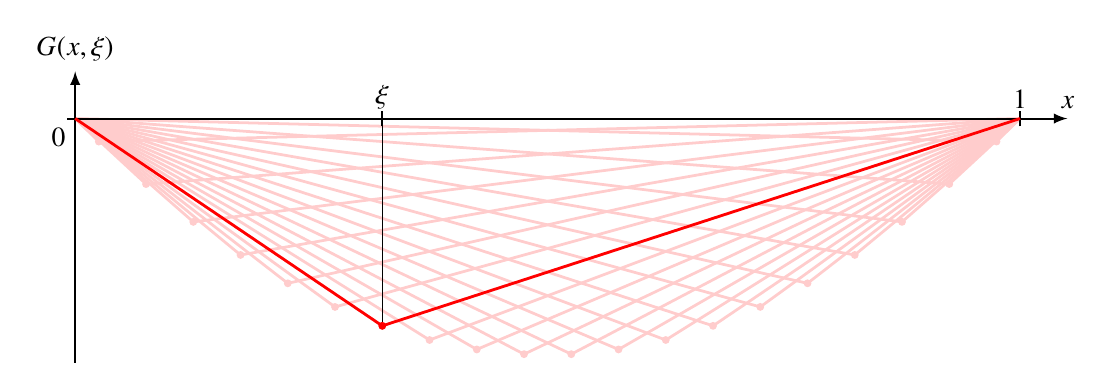
\begin{tikzpicture}[>=latex]

\def\s{12}

\foreach \xi in {0.025,0.075,...,1}{
	\draw[color=red!20,line width=1pt] (0,0)--({\s*\xi},{\s*\xi*(\xi-1)});
	\draw[color=red!20,line width=1pt] ({\s*\xi},{\s*\xi*(\xi-1)})--(\s,0);
	\fill[color=red!20] ({\s*\xi},{\s*\xi*(\xi-1)}) circle[radius=0.05];
}

\draw[->,line width=0.7pt] (-0.1,0)--({\s+0.6},0) coordinate[label=$x$];
\draw[->,line width=0.7pt] (0,{-0.25*\s-0.1})--(0,0.6)
	coordinate[label={$G(x,\xi)$}];

\draw[line width=0.7pt] ({\s},-0.1)--({\s},0.1);
\node at ({\s},0) [above] {$1$};
\node at (0,0) [below left] {$0$};

\def\xiv{0.325}

\draw[line width=0.5pt] ({\s*\xiv},0)--({\s*\xiv},{\s*\xiv*(\xiv-1)});
\draw[line width=0.7pt] ({\s*\xiv},-0.1)--({\s*\xiv},0.1);
\node at ({\s*\xiv},0) [above] {$\xi$};

\draw[color=red,line width=1pt] (0,0)--({\s*\xiv},{\s*\xiv*(\xiv-1)});
\draw[color=red,line width=1pt] ({\s*\xiv},{\s*\xiv*(\xiv-1)})--(\s,0);
\fill[color=red] ({\s*\xiv},{\s*\xiv*(\xiv-1)}) circle[radius=0.05];

\end{tikzpicture}
\end{document}


%
% causality.tex -- 
%
% (c) 2019 Prof Dr Andreas Mueller, Hochschule Rapperswil
%
\section{Causality}
The singular solution $K$ demonstrates that a change in $f$ at
$(t_0,x_0)$ affects all values of the solution $u(t,x)$ for $t>t_0$.
A disturbance at time $t_0$ propagates instantaneously throughout
the the $\Omega$.


%
% eigenfunctions.tex -- 
%
% (c) 2019 Prof Dr Andreas Mueller, Hochschule Rapperswil
%
\section{Eigenfunctions and solutions of the heat equation}
\rhead{Eigenfunctions}
In the previous chapter we have studied the problem
\begin{align*}
\Delta u&=f&&\text{in $\Omega$}\\
u&=g&&\text{on $\partial\Omega$}
\end{align*}
and found that similarly to matrix equations $Ax=b$ Green's function is a kind
of inverse.
Formally, the solution is similar to a matrix equation in the sense
that we just had to replace the sums used in matrix operations by
integrals.

For a parabolic differential equation we have to add time development.
In the framework of a matrix problem, we would have to solve the
equation $\dot x = Ax$, which can be solved by the matrix
exponential function.
The latter is most elegantly computed using eigenvectors, so the
natural questions arises whether we can solve the heat equation
using the eigenvectors of the associated elliptic problem.

This section intends to substantiate this plan.

\subsection{Systems of ordinary differential equation}
The problem analogous to a parabolic partial differential equation
is a ordinary homogeneous linear differential equation for a vector valued
function $t\mapsto x(t)\in\mathbb R^n$.
Such a system can be stated as
\[
\frac{d}{dt}x(t)=Ax(t)
\]
with some constant Matrix $A$.

If tthe matrix $A$ was diagonal, the general solution could be given
immediately as
\[
A=\begin{pmatrix}
\lambda_1&\dots&0\\
\vdots&\ddots&\vdots\\
0&\dots&\lambda_n
\end{pmatrix}
\qquad\Rightarrow\qquad
x(t)=\begin{pmatrix}
x_1(0)e^{\lambda_1t}
\\
\vdots
\\
x_n(0)e^{\lambda_nt}
\end{pmatrix}.
\]
Under certain conditions on the matrix $A$ we can find a set of
orthonormal eigenvectors $e_1,\dots,e_n$.
By using such a vector as initial condition, we get the solution
$e_ie^{\lambda_it}$.
Writing the initial condition as a linear combination
\[
x(0)=\sum_{i=1}^n(e_i \cdot x(0))e_i
\]
of these eigenvectors,
We can immediately write the solution of the differential equation
as a linear combination
\begin{equation}
x(t)=\sum_{i=1}^n
e^{\lambda_i t}
(e_i\cdot x(0))e_i
.
\label{development}
\end{equation}
of the basic solutions.
In fact, substituting this into the differential equation gives
\begin{align*}
\frac{d}{dt}x(t)&=\sum_{i=1}^n\lambda_ie^{\lambda_i t}(e_i\cdot x(0))e_i
\\
Ax(t)
&=\sum_{i=1}e^{\lambda_it}(e_i\cdot x(0))Ae_i
=\sum_{i=1}e^{\lambda_it}(e_i\cdot x(0))\lambda_i e_i
\end{align*}
So for a homogeneous differential equation, eigenvectors immediately
immediately give us the solution.

\subsection{Variation of constants}
The method of variation of constant allows to solve a inhomogeneous
differential equation of first order
\[
\frac{d}{dt}x(t)-Ax(t)=f(t),
\]
for a vector valued function $f$.
For this the constants in the general solution for the homogeneous 
equation are replaced by functions that depend on $t$:
\[
x(t)=\sum_{i=1}^nc_i(t)e^{\lambda_it}e_i.
\]
Substituting this into the differential equation gives
\begin{align*}
\sum_{i=1}^n\dot c_i(t)e^{\lambda_it}e_i
+
\sum_{i=1}^n\lambda_i c_i(t)e^{\lambda_it}e_i
-\sum_{i=1}^n\lambda_i c_i(t)e^{\lambda_it}e_i
&=
f(t)
\\
\sum_{i=1}^n\dot c_i(t)e^{\lambda_it}e_i
&=
f(t)
\end{align*}
By taking the scalar product with the eigenvectors
$e_i$, we get.
\[
\dot c_i(t)e^{\lambda_i t}=(e_i\cdot f(t)).
\]
Abbreviating the right hand side using
$f_i(t)=e_i\cdot f(t)$, turns this into
\[
c_i(t)=c_i(0)+\int_0^te^{-\lambda_i \tau}f_i(\tau)\,d\tau
\]
and the solution becomes
\begin{align*}
x(t)&=
\sum_{i=1}^n
(e_i\cdot x(0))e_i+
\sum_{i=1}^ne^{\lambda_i t}\int_0^te^{-\lambda_i \tau}(e_i\cdot f(\tau))e_i\,d\tau
\\
&=
x(0)
+
\int_0^t
\biggl(
\sum_{i=1}^n
e^{\lambda_i(t- \tau)}(e_i\cdot f(\tau))\biggr)e_i\,d\tau
\end{align*}
One can verify this directly:
\begin{align*}
\frac{d}{dt}x(t)
&=
\sum_{i=1}^n\left.e^{-\lambda_i (t-\tau)}(e_i\cdot f(\tau))e_i \right|_{\tau=t}
\\
&=
\sum_{i=1}^n(e_i\cdot f(t))e_i=f(t)
\end{align*}

\subsection{Eigenvalues and eigenvectors}
Assume now that the domain $\Omega$ is bounded and does not have a 
boundary too complicated, so that there is a sequence of eigenfunctions
$u_i(x)$ of the Laplace operator with eigenvalue $\lambda_i$
with homogeneous boundary conditions, i.~e.
\[
\Delta u_i=\lambda_iu_i,\qquad u_{i|\partial\Omega} = 0.
\]
In addition, we can scale these solutions so that the have 
$L^2$-norm $1$:
\[
\int_{\Omega}|u_i(\xi)|^2\,d\xi=1
\]
The general theory even guarantees that the are orthogonal:
\[
\int_{\Omega}u_i(\xi)u_j(\xi)\,d\xi=0\qquad\forall i\ne j.
\]

We now use these functions in a separation ansatz
$u(x,t)=u_i(x)\cdot T(t)$ for the parabolic equation
\[
\partial_tu=\kappa\Delta u,
\]
and get the equation
\begin{align*}
\partial_t (T(t)u_i(t))-\kappa\Delta(T(t)u_i(t))&=0
\\
T'(t)u_i(t)-\kappa T(t)\Delta u_i(t)&=0
\\
T'(t)u_i(t)-\kappa T(t)\lambda_i u_i(t)&=0
\\
\frac{T'(t)}{T(t)}&=\kappa\lambda_i
\\
\Rightarrow\qquad T(t)=Ce^{\kappa\lambda_it}
\end{align*}
In particular, for initial conditions that are eigenvalues we
immediately get a solution for the parabolic problem.

\subsection{The inhomogeous equation}
The process of variation of constants cann also be used for partial
differential equations.
We write the solution as
\[
u(t,x)=\sum_{i=0}^\infty c_i(t) e^{\kappa\lambda_i t}u_i(x)
\]
and substitute into the differential equation
\begin{align*}
\sum_{i=0}^\infty \dot c_i(t)e^{\kappa\lambda_it}u_i(x)
+\kappa\sum_{i=0}^\infty c_i(t)\kappa\lambda_i e^{\lambda_it}u_i(x)
-\kappa\sum_{i=0}^\infty c_i(t)e^{\kappa\lambda_it}\lambda_iu_i(x)
&=f(x)
\\
\sum_{i=0}^\infty \dot c_i(t)e^{\kappa\lambda_it}u_i(x)
&=f(t,x)
\end{align*}
The scalar product with $u_i$ then gives
\begin{align*}
\dot c_i(t)&= e^{-\kappa\lambda_it}\int_{\Omega}u_i(\xi)f(t,\xi)\,d\xi
\\
c_i(t)&=c_i(0)+\int_0^te^{-\kappa\lambda_i\tau}\int_{\Omega}u_i(\xi)f(\tau,\xi)\,d\xi\,d\tau
\end{align*}
and the particular solution
\begin{align*}
u(t,x)&=
\sum_{i=0}^\infty
u_i(x)
\int_0^t
e^{\kappa\lambda_i(t-\tau)}\int_{\Omega}u_i(\xi)f(\tau,\xi)\,d\xi\,d\tau
\end{align*}
Green's function for the heat equation with Dirichlet boundary conditions
can thus be written as
\[
G(t,x,\tau,\xi)
=
\sum_{i=0}^\infty
e^{\kappa\lambda_i (t-\tau)}
u_i(x)
u_i(\xi).
\]
So we have reduced the solution of the parabolic problem to the
elliptic problem.




%
% hyperbolic.tex -- XXX
%
% (c) 2008 Prof Dr Andreas Mueller
% $Id: c06-hyperbolisch.tex,v 1.3 2008/10/31 08:04:16 afm Exp $
%
\chapter{Hyperbolische Differentialgleichungen\label{chapter-hyperbolisch}}
\index{Differentialgleichung!partielle!hyperbolische}
\index{Wellengleichung}
\lhead{Hyperbolische PDGL}
\rhead{}
In diesem Kapitel wird als prominentes Beispiel einer hyperbolischen
Differentialgleichung die Wellengleichung diskutiert.
Wie im parabolischen Fall hat die Zeitkoordinate eine spezielle Bedeutung,
auch die Wellengleichung ist eine ``Zeitentwicklungsgleichung'', allerdings
zweiter Ordnung. Während sich eine Änderung der Anfangs- oder Randbedingung
bei einem elliptischen Problem sofort überall auf die Lösung auswirkt,
breiten sich solche Änderungen bei der Wellengleichung mit endlicher
Geschwindigkeit aus. Zu jedem Punkt gibt es also Punkte, auf die sich eine
Wertänderung auswirken kann, und andere, die davon nichts mitbekommen.
Die Grenzflächen zwischen diesen Bereichen sind eine wichtige Grundlage
für das Verständnis der Lösungen.

Zunächst werden daher die Lösungen 
am eindimensionalen Fall bestimmt und die in beide Richtungen laufenden 
Wellenlösungen demonstriert. Diese geben Anlass zu einer Untersuchung,
zu welcher Art von Anfangsbedingung die Wellengleichung überhaupt
lösbar ist. Dies führt uns dann auf den Begriff der Charakteristiken.

%
% separation.tex -- XXX
%
% (c) 2019 Prof Dr Andreas Mueller
%
\lhead{Separation der Variablen}
\rhead{}
\chapter{Separation der Variablen\label{chapter-separation}}
\index{Stroboskop}
\index{Eigenschwingung}
\index{stehende Welle}
\begin{figure}
\begin{center}
\includegraphics[width=0.8\hsize]{../common/graphics/stringvibrlarge-10-06-06.jpg}
\end{center}
\caption{Schwingende Saite (Bild von A.~Davidhazy, http://people.rit.edu/andpph/)
\label{separation:schwingendesaite}}
\end{figure}
Beleuchtet man eine schwingende Saite mit einem Stroboskop mit der
Frequenz der Eigenschwingung, scheint die Saite stillzustehen. 
In periodischen Zeit\-ab\-stän\-den sieht die Lösung der Wellengleichung
also gleich aus.
Misst man andererseits die Auslenkung der Saite
an einer Stelle in Abhängigkeit von der Zeit, beobachtet man
eine harmonische Schwingung, die sich mit Hilfe von $\sin$- und
$\cos$-Funktionen beschreiben lässt. Man kann also vermuten,
dass die Lösung der Wellengleichung der schwingenden Saite
ein Produkt
\[
u(x,t)=X(x)\cdot\sin\omega t\quad\text{oder}\quad X(x)\cdot\cos\omega t.
\]
ist. Ziel dieses Kapitels ist, diese Idee zu einem Lösungsverfahren
weiterzuentwickeln und auf einige Differentialgleichungen anzuwenden.

%
% ode.tex -- ordinary differential equations
%
% (c) 2019 Prof Dr Andreas Mueller
%
\section{Separation of Variables for ordinary differential equations}
The differential equation
\begin{equation}
y'-xy=0
\label{separation:ode}
\end{equation}
can be solved using separation of variables:
\begin{align*}
\frac{dy}{dx}&=xy\\
\frac1y\,dy&=x\,dx\\
\int\frac1y\,dy&=\int x\,dx\\
\log|y|&=\frac12x^2+C\\
y&=y_0e^{\frac12x^2}.
\end{align*}
The method is based on the idea to have only a single variable
on either side of the equation.
Even the derivative is formally decomposed as a fraction $dy/dx$, which
isn't really meaningful but justified by the success of the method.
This reduces the solution of the differential equation to the computation
of two integrals, i.~e.~the solution of the particularly simple
differential equation $y'=f(x)$ with solution $y(x)=\int f(x)\,dx$..
This solution also tells us what kind of initial conditions we need
for the solution to be uniquely determined.
If $y_0$ is the value of the solution at $x=x_0$, then the solution is
\[
y(x)=\int_{x_0}^xf(\xi)\,d\xi + y_0.
\]

Of course the process will not be quite as simple when we transition
to partial differential equations.
In particular the suspicious operation to separate the differentials
of $dy/dx$ has no counterpart for more than one independent variable.
However, depending on the shape of the domain, it might still be possible
to separate the variables and to transform the equation into the form
\[
\text{functions/derivatives only involving $x$}
=
\text{functions/derivatives only involving $y$}.
\]
Since the left hand side only depends on $x$ while the right hand side
depends only on $y$, both sides must be constant.
So we can write
\begin{align*}
\text{functions/derivatives only involving $x$} &= \mu
\\
\text{functions/derivatives only involving $y$} &= \mu
\end{align*}
with a new constant $\mu$ that has to be determined later.
This means that we have succeeded to reduce the partial differential
equation to two ordinary differential equations.
Since we know ``all'' about ordinary differential equations, we should
now be in a position to solve the partial differential equation and
to determine what kinds of boundary values are needed to make the
solution unique.


%
% idea.tex -- idea of the method
%
% (c) 2008 Prof Dr Andreas Mueller
%

\section{Idea of the method}
In applications one often has some indications from the application
domain what the solution function will most probably look like, or one
is looking for a very particular type of solution.
In partuclar, it may be known how the solution depends on one of the
variables up to a factor depending only on the other variable.
In these situations one can try to write the solution as a product
or sum of functions that depend on only one variable.

Even if one knows nothing about the solution, one can still try such
an {\em ansatz}, as the following example tries to illustrate.
Let's attempt to solve the partial differetnial equation
\begin{equation}
\frac1x
\frac{\partial u}{\partial x}
+
\frac1y
\frac{\partial u}{\partial y}
=\frac1{y^2}
,
\qquad x>1, y>1,
\label{separation:beispiel1}
\end{equation}
ignoring the boundary conditions for the time being.
We try to represent the solution as a sum of two functions which depend
on one of $x$ and $y$ only.
\begin{equation}
u(x,y)=X(x)+Y(y)
\quad\Rightarrow\quad
\begin{cases}
\quad{\displaystyle \frac{\partial u}{\partial x}}&=X'(x)\\
\\
\quad{\displaystyle \frac{\partial u}{\partial y}}&=Y'(y)\\
\end{cases}
\label{separation:beispiel1:ansatz}
\end{equation}
Substituting this into the differential equation
(\ref{separation:beispiel1})
gives the new equation
\[
\frac{X'(x)}{x}+\frac{Y'(y)}{y}=\frac1{y^2}
\]
or
\begin{equation}
\frac{X'(x)}{x}
=\frac1{y^2}
-\frac{Y'(y)}{y}.
\label{separation:beispiel1:separiert}
\end{equation}
The Form (\ref{separation:beispiel1:separiert}) has a distinct property:
the variable $x$ only appears on the left side, the variable $y$ only on
the right.
If we fix some value $y$, the right hand side cannot change, so the left
hand side must not depend on $x$.
Conversely, if we fix $x$, then the left side cannot change any more,
and thus the right hand side cannot change either.
We conclude that both sides must be the same constant.
Calling this constant $k$ we find the two ordinary differential equations
\begin{align}
\frac{X'(x)}{x}&=k
&
k&=\frac1{y^2}-\frac{Y'(y)}{y}
\label{separation:beispiel1:separiertedgl}
\end{align}
for $X(x)$ and $Y(y)$.

The differential equation for $X$ is easy to solve:
\begin{align*}
X'(x)&=kx\quad\Rightarrow\quad X(x)=
\frac12kx^2+C_x.
\end{align*}
The right equation is only slightly more complicated:
\begin{align*}
Y'(y)=\frac1y-ky
\quad\Rightarrow\quad
Y(y)=\int\frac1y-ky\,dy=
\log y-\frac12ky^2+C_y.
\end{align*}
We can now combine these functions into a solution of the initial
differential equation:
\begin{equation}
u(x,y)=
\frac12kx^2+
\log y-\frac12ky^2+C.
\label{separation:beispiel1:loesung}
\end{equation}
By varying the parameters $k$ and $C$, formula
(\ref{separation:beispiel1:loesung}) gives an infinite family of
solutions of the partial differential equation.

The values of the constants need to be determined by boundary conditions
in a manner to be studied later.

Let's summarize the method so far:
\begin{enumerate}
\item
Choose an {\em ansatz} from functions that depend from disjoint
sets of variables.
\item
Substitute into the partial differential equation and separate terms
involving the separate sets of variables.
The two sides of the equation depend on disjoint sets of variables
und must therefore be constant.
\item 
Split the equation into two coupled equations, each with a
different set of independent variables.
\item
Solve each equation individually.
\item
Put solutions together using the boundary conditions.
\end{enumerate}
As may suspected, the problem most of the time is not the solution
of the individual equations but rather the last step.
In the following sections we want to illustrate how this can be
done in a variety of examples.


%
% lpde.tex -- why linear pdes?
%
% (c) 2019 Prof Dr Andreas Mueller
%
\section{Separation for linear partial differential equations}
The base idea of the separation method produces a family of functions
that depend an some integration and separation constants.
On the boundary we are usually given some arbitrary functions.
In general it will be impossible to tune these few constants to
values that reproduce the boundary functions.
This basic version of the separation method thus is incapable of
solving a general partial differential equation due to the lack
of flexibility in the set of solutions found.

This problem changes if different solutions can be combined into new ones.
Linear combinations of solutions introduce a large set of additional
parameters to tune the solution.
In particular, Fourier theory shows that linear combinations of
basic functions can be tuned to approximate just about any periodic
function.
However, linear combinations of solutions are in general no longer
solutions the equation, except for linear partial differential
equations.
This is expressed in the following theorem.

\begin{satz}
If $u_1$ and $u_2$
are solutions of a homogeneous linear partial differential equation,
then $u_1+u_2$ and $\lambda u_1$ with $\lambda\in\mathbb R$ are also
solutions.
\end{satz}

\begin{proof}
The differential equation
\[
F(x_1,\dots,x_2,u,\frac{\partial u}{\partial x_1},\dots)=0
\]
is linear in $u$ and its derivatives, so we can expand sums and
pull factors from inside $F$:
\begin{align*}
F(x_1,\dots,x_2,u_1+u_2,\frac{\partial u_1}{\partial x_1}+\frac{\partial u_2}{\partial x_1},\dots)
&=
F(x_1,\dots,x_2,u_1,\frac{\partial u_1}{\partial x_1},\dots)
\\
&+
F(x_1,\dots,x_2,u_2,\frac{\partial u_2}{\partial x_1},\dots)=0
\\
F(x_1,\dots,x_2,\lambda u_1,\frac{\partial \lambda u_1}{\partial x_1},\dots)
&=
\lambda
F(x_1,\dots,x_2,u_1,\frac{\partial u_1}{\partial x_1},\dots)
=0
\end{align*}
Thus linear combinations of $u_1$ and $u_2$ are solutions too.
\end{proof}

Linear cominations allow us to first find as many different solutions
$u_1$, $u_2$, $u_3,\dots$ and then to use suitable coefficients $a_k$
to combine them into a solution
\[
u(x)=\sum_{i=1}^\infty a_ku_k
\]
that also satisfies the boundary conditions.

Inhomogeneous linear partial differential equations can be solved using
this method too.
As pointed out in chapter~\ref{chapter:terminology-and-notation},
we first have to find a particular solution $u_p$ which solves the
inhomogeneous partial differential equation independently
of any boundary conditions.
The separation method can be helpful for this too.
Then the problem is reduced to finding a solutions $u_h$ to the homogeneous
equations with boundary condition $g-u_p$ on $\partial\Omega$.
Using the separation method, we can build up $u_h$ as a linear combination
of solutions.

The coefficients $a_k$ for the linear combination often lead us into
Fourier theory or some generalization of it.
Such partial solutions often have immediate physical significance.
In mechanical or electrical engineering they appear as vibration modes,
in quantum mechanics as energy states.



%
% membrane.tex -- XXX
%
% (c) 2019 Prof Dr Andreas Mueller
%
\section{Schwingende rechteckige Membran}
\rhead{Rechteckige Membran}
\index{Membran!rechteckig}
Wir betrachten die Schwingung einer rechteckigen Membran, die am Rande
des Gebietes
\[
R=\{(x,y)\,|\,0\le x\le a,0\le y\le b\} =(0,a)\times(0,b)
\]
eingespannt ist. Zur Zeit $t=0$ sei die Form der Membran durch die
Funktion $f(x,y)$ gegeben.
Für beliebige Zeit $t\ge 0$ wird sie beschrieben durch eine Funktion $u(x,y,t)$,
welche der Differentialgleichung
\[
\frac1{c^2}\frac{\partial^2u}{\partial t^2}=\frac{\partial^2u}{\partial x^2}+\frac{\partial^2u}{\partial y^2}
\]
genügt mit den Anfangsbedingungen
\begin{align*}
u(x,y,0)&=f(x,y)\quad\forall 0\le x\le a,0\le y\le b,
\\
\frac{\partial}{\partial t}u(x,y,0)&=g(x,y)\quad\forall 0\le x\le a,0\le y\le b
\end{align*}
und den Randbedingungen
\begin{align*}
u(0,y,t)&=0&u(a,y,t)&=0&\forall t\ge 0,0\le y\le b,\\
u(x,0,t)&=0&u(x,b,t)&=0&\forall t\ge 0,0\le x\le a.
\end{align*}

\subsection{Separation der Zeit}
\index{Separation}
Nach der in der Einleitung motivierten Idee suchen wir Lösungen also
Produkt einer Funktion $T(t)$, die nur von der Zeit abhängt, und einer Funktion
$\varphi(x,y)$, welche nur vom Ort abhängt, also
\[
u(x,y,t)=T(t)\cdot\varphi(x,y).
\]
Leider kann ein einzelnes solches Produkt nicht alle Anfangsbedingungen
erfüllen. Wäre dies nämlich möglich, müsste $\varphi(x,y)\sim f(x,y)$
sein und alle Teile der Membran würden im Gleichtakt hin und her schwingen.
Simulationen oder physikalische Experimente zeigen aber, dass es
Anfangsbedingungen gibt, bei denen die Teile der Membran gegenläufig
schwingen.

Anderseits, muss die Lösung auf jeden Fall die Randbedingung erfüllen,
es muss also gelten
\begin{align*}
\varphi(0,y)&=0&\varphi(a,y)&=0&0\le y\le b\\
\varphi(x,0)&=0&\varphi(x,b)&=0&0\le x\le a
\end{align*}
Setzen wir diesen Ansatz für $u$ in der Wellengleichung ein,
erhalten wir
\[
\frac1{c^2}T''(t)\varphi(x,y)=T(t)\left(
\frac{\partial^2\varphi}{\partial x^2}
+
\frac{\partial^2\varphi}{\partial y^2}
\right)
\]
Wir suchen eine Funktion $u$, die nicht identisch verschwindet,
es gibt also einige Zeitpunkte $t$ und Orte $(x,y)$, an denen $T(t)$
und $\varphi(x,y)$ nicht verschwinden. An diesen Stellen kann man die
Gleichung umformen in
\begin{equation}
\frac1{c^2}\frac{T''(t)}{T(t)}
= \frac1{\varphi(x,y)}\left( \frac{\partial^2\varphi}{\partial x^2}
+ \frac{\partial^2\varphi}{\partial y^2} \right)
\label{separiertMembran}
\end{equation}
Die rechte Seite hängt nur
vom Ort ab, darf sich also nicht ändern, wenn man die Zeit $t$ variert.
Als Funktion der Zeit muss die linke Seite eine Konstante sein,
es gibt also ein $k$ mit der Eigenschaft
\[
\frac1{c^2}\frac{T''(t)}{T(t)}=k
\qquad\Leftrightarrow\qquad
T''(t)=k T(t).
\]
Diese gewöhnliche Differentialgleichung hat Lösungen der Form 
$e^{\pm\sqrt{k}t}$ für positives $k$. Für negatives $k$ sind $\sin\sqrt{k}t$ 
und $\cos\sqrt{k}t$ Lösungen.
Aus physikalischer Sicht sind nur Lösungen mit Schwingungscharakter sinnvoll,
wir können daher annehmen, dass $k<0$.
Ein solches $k$ lässt sich in der Form $k=-\lambda^2$ schreiben.
Es gibt also ein $\lambda$ mit der Eigenschaft
\[
\frac1{c^2}\frac{T''(t)}{T(t)}=-\lambda^2
\]
oder
\[
T''(t)=-c^2\lambda^2 T(t).
\]
Dies ist eine gewöhnliche Differentialgleichung zweiter Ordnung, welche mit
bekannten Methoden gelöst werden kann.
Die allgemeine Lösung dieser Gleichung ist von der Form
\[
A\cos c\lambda t+B\sin c\lambda t.
\]

\subsection{Reduktion auf ein Eigenwertproblem}
\index{Eigenwertproblem}
Die linke Seite von (\ref{separiertMembran}) hängt nur von der Zeit ab, darf sich
also nicht ändern, wenn man $x$ oder $y$ variert. Als Funktion des Ortes
muss die rechte Seite also ebenfalls konstant sein:
\begin{align*}
\frac1{\varphi(x,y)}\left(
\frac{\partial^2\varphi}{\partial x^2}
+
\frac{\partial^2\varphi}{\partial y^2}
\right)&=-\lambda^2\\
\frac{\partial^2\varphi}{\partial x^2}
+
\frac{\partial^2\varphi}{\partial y^2}
=\Delta\varphi
&=-\lambda^2
\varphi(x,y)
\end{align*}
Die gesuchte Funktion $\varphi$ ist also ein Eigenvektor des linearen
Operators $\Delta$ zum Eigenwert $-\lambda^2$.
Nur die Eigenwerte des Operator $\Delta$ kommen also für die
Zeitabhängigkeitsgleichung in Frage.

\subsection{Separation von $x$ und $y$}
\index{Separation}
Für das Eigenwertproblem können wir erneut den Separationsansatz
\[
\varphi(x,y)=X(x)\cdot Y(y)
\]
versuchen.
Einsetzen in die Differentialgleichung ergibt
\begin{align*}
X''(x)Y(x)+X(x)Y''(y)&=-\lambda^2 X(x)Y(y)
\\
\frac{X''(x)}{X(x)}+\frac{Y''(y)}{Y(y)}&=-\lambda^2
\end{align*}
Jeder der Brüche hängt nur von jeweils einer Variable ab, was nur
möglich ist, wenn beide Terme konstant sind. Damit ist das Problem
reduziert auf zwei Gleichungen
\begin{align*}
X''(x)&=-\lambda_1^2X(x)\\
Y''(y)&=-\lambda_2^2Y(y)\\
\lambda_1^2+\lambda_2^2&=\lambda^2
\end{align*}
Die allgemeinen Lösungen dieser Gleichungen, die auch die Randbedingung
bei $x=0$ bzw.~$y=0$ erfüllt, sind
\begin{align*}
X(x)&=A\sin \lambda_1x\\
Y(y)&=B\sin \lambda_2y
\end{align*}
Die Randbedingungen für $x=a$ und $y=b$ können nur erfüllt werden,
wenn $\lambda_1a$ und $\lambda_2b$ Vielfache von $\pi$ sind, also
\[
\lambda_1=\frac{k\pi}a
\qquad
\text{und}
\qquad
\lambda_2=\frac{l\pi}b
\]
Die möglichen Werte von $\lambda$ sind also
\[
\lambda_{kl}^2=\left(\frac{k^2}{a^2} + \frac{l^2}{b^2}\right)\pi^2,\qquad k,l\in\mathbb Z
\]
Damit kann man jetzt die allgemeine Lösung des Schwingungsproblems aus den
Teillösungen
\[
\varphi_{kl}(x,y)=\sin \frac{k\pi}{a}x\sin\frac{l\pi}{b}y
\]
für das Eigenwertproblem
und den Teillösungen
\[
u_{kl}(x,y,t)
=
(A_{kl}\cos c\lambda_{kl} t+
B_{kl}\sin c\lambda_{kl} t)
\sin \frac{k\pi}{a}x\sin\frac{l\pi}{b}y
\]
für das zeitabhängige Problem
zu einer allgemeinen Lösung
\begin{equation}
u(x,y,t)=\sum_{k,l}
(A_{kl}\cos c\lambda_{kl} t+
B_{kl}\sin c\lambda_{kl} t)
\sin \frac{k\pi}{a}x\sin\frac{l\pi}{b}y
\label{allgemeineloesung}
\end{equation}
zusammensetzen.

\subsection{Anfangsbedingungen}
\index{Anfangsbedingungen}
Die allgemeine Lösung muss jetzt auch noch die Anfangsbedingung erfüllen:
\begin{align*}
\sum_{k,l}A_{kl}
\sin \frac{k\pi}{a}x\sin\frac{l\pi}{b}y&=f(x,y)\\
\sum_{k,l}B_{kl}c\lambda_{kl}
\sin \frac{k\pi}{a}x\sin\frac{l\pi}{b}y&=g(x,y)\\
\end{align*}
Die Koeffizienten $A_{kl}$ und $B_{kl}$ können in einfachen Fällen mit
Koeffizientenvergleich und im Allgemeinen mit Hilfe der Theorie
der Fourierreihen berechnet werden.
\index{Fourierreihe}


%
% disk.tex -- XXX
%
% (c) 2019 Prof Dr Andreas Mueller
%
\section{Kreisgebiet}
\rhead{Kreisgebiet}
\index{Kreisgebiet}
\index{Kreisscheibe}
In diesem Abschnitt betrachten wir eine Kreisscheibe
\[
G=\{(x,y)\in\mathbb R^2|x^2+y^2 < R\}
\]
mit Radius $R$ als Definitionsbereich. Da sich dieses Gebiet durch
eine Streckung um den Faktor $\frac1R$ immer auf einen Einheitskreis
abbilden lässt, können wir ohne Verlust an Allgemeinheit vorausetzen,
dass $R=1$ ist.

Ein Kreisgebiet tritt zum Beispiel beim Problem auf, die Schwingungen
einer kreisförmigen Membran zu berechnen, wie sie bei einer Kesselpauke
vorkommen. Nach den Ergebnissen des ersten Kapitels suchen wir nach einer
Funktion $u$, welche auf $G$ die Gleichung
\[
\frac1{a^2}\frac{\partial^2 u}{\partial t^2}=\frac{\partial^2 u}{\partial x^2}+\frac{\partial^2 u}{\partial y^2}
\]
erfüllt. Wie bei der Schwingung der einer rechteckigen Platte
wird daraus mit dem Ansatz $ u(x,y,t)=u(x,y)\cdot T(t)$ ein
Eigenwertproblem:
\begin{align*}
T''(t)&=-a^2\lambda^2 T(t)\\
\Delta u(x,y)&=-\lambda^2u(x,y)
\end{align*}
Das Poissonproblem ist der Spezialfall $\lambda=0$.
\index{Poissonproblem}

\subsection{Polarkoordinaten}
\index{Polarkoordinaten}
Offenbar sind Polarkoordinaten speziell gut an das Problem angepasst, 
eine Randbedingung lässt sich zum Beispiel durch eine Funktion beschreiben,
welche nur vom Polarwinkel abhängt.
Eine schwingende kreisförmite Membran führt also auf die partielle
Differentialgleichung
\[
\frac{\partial^2u(r,\varphi)}{\partial t^2}=\Delta u(r,\varphi)
\]
mit der Randbedingung
\[
u(R,\varphi)=0,\qquad\varphi\in[0,2\pi],
\]
wobei wie oben $R$ der Radius der Membran ist.

Damit das Problem auf einem Kreisgebiet in Polarkoordinaten behandelt
werden kann,
brauchen wir einen Ausdruck für $\Delta u$ in Polarkoordinaten.
\begin{align}
x&=r\cos\varphi\\
y&=r\sin\varphi
\label{polarkoordinaten}
\end{align}
Um die Ableitungen nach $x$ und $y$ durch Ableitungen $\varphi$ und $r$ zu
ersetzen, leiten wir (\ref{polarkoordinaten}) nach $x$ und $y$ ab:
\begin{align*}
1&=
\frac{\partial r}{\partial x}\cos\varphi
-r\sin\varphi \frac{\partial\varphi}{\partial x}
&
0&=
\frac{\partial r}{\partial y}\cos\varphi
-r\sin\varphi \frac{\partial\varphi}{\partial y}
\\
0&=
\frac{\partial r}{\partial x}\sin\varphi
+r\cos\varphi \frac{\partial\varphi}{\partial x}
&
1&=
\frac{\partial r}{\partial y}\sin\varphi
+r\cos\varphi \frac{\partial\varphi}{\partial y}
\end{align*}
In Matrixschreibweise ist dies
\begin{align*}
\begin{pmatrix}1\\0\end{pmatrix}
&=
\begin{pmatrix}
\cos\varphi&-\sin\varphi\\
\sin\varphi&\cos\varphi
\end{pmatrix}
\begin{pmatrix}
\frac{\partial r}{\partial x}\\
r\frac{\partial \varphi}{\partial x}
\end{pmatrix}
&
\begin{pmatrix}0\\1\end{pmatrix}
&=
\begin{pmatrix}
\cos\varphi&-\sin\varphi\\
\sin\varphi&\cos\varphi
\end{pmatrix}
\begin{pmatrix}
\frac{\partial r}{\partial y}\\
r\frac{\partial \varphi}{\partial y}
\end{pmatrix}
\end{align*}
Die $2\times2$ Matrix ist eine Drehmatrix, die Inverse findet man, indem man
$\varphi$ durch $-\varphi$ ersetzt. Die Multiplikation auf der linken Seite
ergibt jeweils die erste bzw. zweite Spalte der Drehmatrix zum
Winkel $\varphi$:
\begin{align*}
\cos\varphi
&=\frac{\partial r}{\partial x}
&&
&
\sin\varphi
&=
\frac{\partial r}{\partial y}
&&
\\
-\sin\varphi
&=r\frac{\partial \varphi}{\partial x}
&\Rightarrow\quad
\frac{\partial\varphi}{\partial x}&=-\frac1r\sin\varphi
&
\cos\varphi
&=
r\frac{\partial\varphi}{\partial y}
&\Rightarrow\quad
\frac{\partial\varphi}{\partial y}&=\frac1r\cos\varphi
\end{align*}
Mit diesen Formeln können wir jetzt die höheren Ableitungen
von $u$ nach  $x$ und $y$ durch Ableitungen nach $r$ und $\varphi$
ersetzen.

Die partiellen Ableitungen von $\varphi$ nach $x$ und $y$ sind
\begin{align*}
\frac{\partial u}{\partial x}
&=
\frac{\partial u}{\partial r}
\frac{\partial r}{\partial x}
+
\frac{\partial u}{\partial\varphi}
\frac{\partial \varphi}{\partial x}
=
\frac{\partial u}{\partial r}
\cos\varphi
-
\frac{\partial u}{\partial\varphi}
\frac1r\sin\varphi
\\
\frac{\partial u}{\partial y}
&=
\frac{\partial u}{\partial r}
\frac{\partial r}{\partial y}
+
\frac{\partial u}{\partial\varphi}
\frac{\partial \varphi}{\partial y}
=
\frac{\partial u}{\partial r}
\sin\varphi
+
\frac{\partial u}{\partial\varphi}
\frac1r\cos\varphi
\end{align*}
Die zweiten Ableitungen sind
\begin{align*}
\frac{\partial^2u}{\partial x^2}
&=
\frac{\partial}{\partial r}
\left(
\frac{\partial u}{\partial r}
\cos\varphi
-
\frac{\partial u}{\partial\varphi}
\frac1r\sin\varphi
\right)
\frac{\partial r}{\partial x}
+
\frac{\partial }{\partial \varphi}
\left(
\frac{\partial u}{\partial r}
\cos\varphi
-
\frac{\partial u}{\partial\varphi}
\frac1r\sin\varphi
\right)
\frac{\partial\varphi}{\partial x}
\\
&=
\frac{\partial}{\partial r}
\left(
\frac{\partial u}{\partial r}
\cos\varphi
-
\frac{\partial u}{\partial\varphi}
\frac1r\sin\varphi
\right)
\cos\varphi
-
\frac{\partial }{\partial \varphi}
\left(
\frac{\partial u}{\partial r}
\cos\varphi
-
\frac{\partial u}{\partial\varphi}
\frac1r\sin\varphi
\right)
\frac1r\sin\varphi
\\
&=
\frac{\partial^2u}{\partial r^2} \cos^2\varphi
-
\frac{\partial^2u}{\partial r\partial\varphi} \frac1r\sin\varphi \cos\varphi
+
\frac{\partial u}{\partial\varphi} \frac1{r^2}\sin\varphi\cos\varphi
\\
&\quad
-
\frac{\partial^2u}{\partial\varphi\partial r}\frac1r \cos\varphi\sin\varphi
+\frac{\partial u}{\partial r}\frac1r\sin^2\varphi
+\frac{\partial^2u}{\partial\varphi^2}
\frac1{r^2}\sin^2\varphi
+\frac{\partial u}{\partial\varphi}\frac1{r^2}\cos\varphi\sin\varphi
\\
\frac{\partial^2u}{\partial y^2}
&=
\frac{\partial}{\partial r}
\left(
\frac{\partial u}{\partial r}
\sin\varphi
+
\frac{\partial u}{\partial\varphi}
\frac1r\cos\varphi
\right)
\frac{\partial r}{\partial y}
+
\frac{\partial}{\partial \varphi}
\left(
\frac{\partial u}{\partial r}
\sin\varphi
+
\frac{\partial u}{\partial\varphi}
\frac1r\cos\varphi
\right)
\frac{\partial \varphi}{\partial y}
\\
&=
\frac{\partial}{\partial r}
\left(
\frac{\partial u}{\partial r}
\sin\varphi
+
\frac{\partial u}{\partial\varphi}
\frac1r\cos\varphi
\right)
\sin\varphi
+
\frac{\partial}{\partial \varphi}
\left(
\frac{\partial u}{\partial r}
\sin\varphi
+
\frac{\partial u}{\partial\varphi}
\frac1r\cos\varphi
\right)
\frac1r\cos\varphi
\\
&=
\frac{\partial^2u}{\partial r^2}\sin^2\varphi
+\frac{\partial^2u}{\partial r\partial\varphi}\frac1r\cos\varphi\sin\varphi
-\frac{\partial u}{\partial\varphi}\frac1{r^2}\cos\varphi\sin\varphi
\\
&\quad
+
\frac{\partial^2u}{\partial\varphi\partial r}\frac1r\sin\varphi\cos\varphi
+\frac{\partial u}{\partial r}\frac1r\cos^2\varphi
+\frac{\partial^2u}{\partial \varphi^2}\frac1{r^2}\cos^2\varphi
-\frac{\partial u}{\partial \varphi}\frac1{r^2}\sin\varphi\cos\varphi
\end{align*}
\index{Laplace-Operator!in Polarkoordinaten}
Die Summe dieser zwei Terme ist die gesucht Darstellung des Laplace-Operators
in Polarkoordinaten:
\begin{align*}
\frac{\partial^2u}{\partial x^2}+\frac{\partial^2u}{\partial y^2}
&=
\frac{\partial^2u}{\partial r^2}
+\frac{\partial u}{\partial r}\frac1r
+\frac{\partial^2u}{\partial\varphi^2}\frac1{r^2}
\\
&=
\left(\frac1r\frac{\partial}{\partial r}r\frac{\partial}{\partial r}+\frac1{r^2}\frac{\partial^2}{\partial \varphi^2}\right)u
\end{align*}
Darstellungen des Laplace-Operators in weiteren Koordinatensystemen können
in jeder einigermassen vollständigen Formelsammlung gefunden werden.

\subsection{Separation der Ortsvariablen}
Die Lösung $u(r,\varphi)$ des Eigenwertproblems setzen wir wieder
als Produkt einer Funktion
$R(r)$
nur von  $r$ und einer Funktion $\Phi(\varphi)$ nur von $\varphi$ an.
Mit der im vorangegangenen Abschnitt gefundenen Formel für den Laplace-Operator
in Polarkoordinaten erhalten wir jetzt die Gleichungen
\begin{align*}
\Delta u=
\biggl(R''(r) + \frac1rR'(r)\biggr)\Phi(\varphi)
+\frac1{r^2}R(r)\Phi''(\varphi)&=-\lambda^2 R(r)\cdot\Phi(\varphi)\\
\frac{r^2R''(r)+rR'(r)}{R(r)}+\frac{\Phi''(\varphi)}{\Phi(\varphi)}
&=-\lambda^2 r^2
\\
\frac{r^2R''(r)+rR'(r)}{R(r)}+\lambda^2 r^2&=-\frac{\Phi''(\varphi)}{\Phi(\varphi)}
\end{align*}
Da die rechte Seite nur von $\varphi$ abhängt, die linke Seite aber nur von $r$,
müssen beide Seiten konstant sein, wir nennen diese Konstante $\mu^2$.
Damit sind die Variablen separiert:
\begin{align}
\Phi''(\varphi)+\mu^2\Phi(\varphi)&=0\label{phigleichung}\\
r^2R''(r)+rR'(r)+(\lambda^2 r^2-\mu^2)R(r)&=0\label{rgleichung}
\end{align}

\subsection{Lösung der separierten Differentialgleichungen}
Die allgemeine Lösung der Gleichung (\ref{phigleichung}) ist
\[
\Phi(\varphi)=A\cos\mu\varphi +B\sin\mu\varphi.
\]
Dies ist nur dann $2\pi$-periodisch, wenn $\mu$ eine ganze
Zahl ist, also $\mu=k$ mit $k\in\mathbb Z$.

Die Gleichung (\ref{rgleichung}) für $R$ bekommt damit die Form
\[
r^2R''(r)+rR'(r)+(\lambda^2 r^2-k^2)R(r)=0,
\]
sie ist verwandt mit der Besselschen Differentialgleichung.
Die Funktion $P(\varrho)=R(\varrho/\lambda)=R(r)$ hat die Ableitungen
\begin{align*}
\varrho P'(\varrho)&=\frac{\varrho}{\lambda}R'(\varrho/\lambda)=rR'(r)\\
\varrho^2 P''(\varrho)&=\frac{\varrho^2}{\lambda^2}R'(\varrho/\lambda)=r^2R''(r)
\end{align*}
und erfüllt somit die Besselsche Differentialgleichung
\[
\varrho^2P''(\varrho)+\varrho P'(\varrho)+(\varrho^2-k^2)P(\varrho).
\]
Lösungen der Besselschen Differentialgleichungen sind die Besselfunktionen
\[
P(\varrho)=J_{\pm k}(\lambda r)=R(r)
\]
Wie bei der rechteckigen Membran kann die allgemeine Lösung jetzt aus
den Teillösungen zusammengesetzt werden.


%
% initial.tex -- XXX
%
% (c) 2019 Prof Dr Andreas Mueller
%
\rhead{Anfangsbedingungen}
\section{Anfangsbedingungen}
In den bisherigen Beispielen haben wir Lösungen einer partiellen
Differentialgleichung gesucht und gefunden, welche bestenfalls einen
Teil der Randbedingungen erfüllt haben.
So haben wir zwar sichergestellt, dass die schwingende Membran eingespannt
bleibt, aber die Auslenkung der Membran zu Beginn haben wir ignoriert.

Um zu verstehen, wie die Anfangsbedingungen ebenfalls berücksichtig
werden können, betrachten wir die Wellengleichung
\[
\frac{\partial^2 u}{\partial t^2}=\frac{\partial^2 u}{\partial x^2}
\]
auf dem Gebiet $(t,x)\in\mathbb R\times [0,\pi]$
mit den Randbedingungen
\[
u(t,0)=u(t,\pi)=0.
\]
Wir verwenden den Separationsansatz
$u(t,x)=T(t)\cdot X(t)$, welcher uns wie früher dargestellt auf eine
Gleichung
\[
\frac{T''(t)}{T(t)}=\frac{X''(x)}{X(x)}=-\lambda^2
\]
führt.
Die Gleichung 
\[
X''(x)=-\lambda^2 X(x)
\]
hat als Lösung Linearkombinationen von Sinus- und Kosinusfunktionen
\[
X(x)=A\cos\lambda x+B\sin\lambda x.
\]
Damit die Anfangsbedingung am linken Rand erfüllt ist, muss $A=0$
sein. Am rechten Rand bleibt daher nur $B\sin\lambda \pi$, und wir
müssen $B\ne 0$ annehmen, da sonst die ganze Lösung verschwinden
würde. $\sin\lambda \pi$ wird aber nur dann verschwinden, wenn
$\lambda$ eine ganze Zahl ist, also
\[
X_k(x)=B\sin kx, \quad 0<k\in\mathbb Z.
\]
Die dazu passende Lösung von $T''(t)=-k^2T(t)$ hat genau die
gleiche Form, so dass die allgemeine Lösung zum Wert $\lambda=k$
\[
u_k(t,x)=\sin kx\left(A_k\cos kt+B_k\sin kt\right)
\]
ist.

Diese Teillösungen $u_k(t,x)$ erfüllen bereits die Differentialgleichung
und die Randbedingungen. Noch nicht erfüllt werden die Anfangsbedingungen
zur Zeit $t=0$. Wir geben sie in der Form
\begin{align*}
u(0,x)&=f(x)\quad x\in[0,\pi]\\
\frac{\partial u}{\partial t}(0,x)&=g(x)\quad x\in[0,\pi]
\end{align*}
vor.

Wir suchen jetzt also eine Lösung in der Form
\[
u(t,x)=\sum_{k=1}^{\infty}
\left(A_k\cos kt+B_k\sin kt\right)
\sin kx,
\]
welche die Anfangsbedingung erfüllt. Durch Einsetzen erhält
man
\begin{align*}
\sum_{k=1}^{\infty}
A_k \sin kx
&=f(x)
\\
\sum_{k=1}^{\infty}
B_kk\sin kx
&=g(x)
\end{align*}
für $x\in[0,\pi]$.
Die Lösung $u(t,x)$ kann also vollständig bestimmt werden, indem man
die Anfangsbedingungen in eine Fourier-$\sin$-Reihe entwickelt. Sind
$\hat f(k)$ und $\hat g(k)$ die Fourier-Koeffizienten, wird die
vollständige Lösung
\[
u(t,x)
=
\sum_{k=1}^{\infty}(\hat f(k)\cos kt+\hat g(k)k\sin kt)\sin kx.
\]
Mit geeigneten Voraussetzungen an die Funktionen $f$ und $g$ werden
diese Reihen konvergieren.


%
% summary.tex -- XXX
%
% (c) 2019 Prof Dr Andreas Mueller
%
\section{Zusammenfassung: Separationsverfahren}
Aus diesen Beispielen lässt sich jetzt das allgemeine Prinzip 
ableiten. Gegeben ist eine partielle Differentialgleichung
beliebiger Ordnung mit unabhängigen Variablen $x_1,\dots,x_n$.
Ziel ist, die Differentialgleichung auf eine solche mit weniger
unabhängigen Variablen zu reduzieren. Sobald man die Reduktion
bis auf eine Variable geschafft hat, hat man die partielle
Differentialgleichung in gewöhnliche Differentialgleichungen
umgewandelt, typischerweise in Randwertprobleme,
die man mit gekannten Techniken lösen kann.

Da man am Schluss die Lösung aus den Teillösungen zusammensetzen
muss, die die separierten Gleichungen liefern, ist dieses Vorgehen
nur bei linearen PDGL sinnvoll. Wir gehen also im folgenden von
einer linearen PDGL aus.

Wir gehen also von einer Differentialgleichung für die Funktion
$u(x_1,\dots,x_n)$ aus, und wollen die Variable $x_1$ separieren.
Dazu geht man wie folgt vor.
\begin{enumerate}
\item Setzt die Lösung $u$ der Differentialgleichung in der
Form eines Produktes an:
\[
u(x_1,\dots,x_n)=X_1(x_1)u_1(x_2,\dots,x_n).
\]
\item Einsetzen des Ansatzes in die Differentialgleichung.
\item
Mit etwas Glück lassen sich die Terme, die
$X_1$ und $u_1$ enthalten trennen und auf verschiedene Seiten
des Gleichheitszeichens bringen.
Da die Lösung $u\equiv 0$ nicht interessant ist, kann man
zu diesem Zweck durch $u$ dividieren, die Gleichung muss
ausserhalb der Nullstellen von $u$ immer noch erfüllt sein.
Die Gleichung hat jetzt also die Form
\[
F(x_1,X_1,X_1',\dots,X_1^{(n)})
=
G(x_2,\dots,x_n,u_1,\partial_2u_1,\dots\partial_nu_n,\dots)
\]
\item
Da die linke Seite nur von $x_1$, die rechte nur von $x_2,\dots,x_n$
abhängt, müssen beide Konstant sein, wir haben also die ursprüngliche
PDGL in zwei Differentialgleichungen zerlegt:
\begin{equation}
\begin{aligned}
F(x_1, X_1,X_1',\dots, X_1^{(n)})&=k\\
G(x_2,\dots,x_n,u_1,\partial_2u_1,\dots\partial_nu_n,\dots)&=k
\end{aligned}
\label{separiert}
\end{equation}
wobei $k$ eine Konstante ist.
Dies sind zwei Differentialgleichungen, die erste ist eine
gewöhnliche Differntialgleichung, und falls $n>2$ ist die zweite
eine partielle Differentialgleichung, die unter Umständen noch
einmal mit dem gleichen Verfahren behandelt werden muss.
Gesucht werden alle Konstanten,
für welche beide Gleichungen eine Lösung haben.
\item Sind $X_1(k,x_1)$ und $u_1(k,x_2,\dots,x_n)$ Lösungen der
Gleichungen (\ref{separiert}), dann sind 
\[
u_k(x_1,\dots,x_n)=X_1(k,x_1)u_1(k,x_2,\dots,x_n)
\]
Lösungen der ursprünglichen PDGL. Die allgmeine Lösung ist daher
eine Summe
\[
u(x_1,\dots,x_n)=
\sum_{k}
a_k
u_k(x_1,\dots,x_n)=X_1(k,x_1)u_1(k,x_2,\dots,x_n),
\]
wobei die Summe über die möglichen $k$ zu erstrecken ist.
\item
Zur Erfüllung von Randbedingungen müssen jetzt die Koeffizienten
$a_k$ bestimmt werden, für die die Randtterme korrekt werden.
\end{enumerate}
Das Verfahren kann an zwei Stellen zusammenbrechen:
\begin{itemize}
\item In Schritt 3 wird vorausgesetzt, dass die Trennung in 
Terme, die $x_1$ enthalten  und solche, die $x_1$ nicht enthalten
möglich ist. Dies ist nicht automatisch der Fall, kann aber in
vielen praktisch wichtigen Fällen durch Wahl eines geeigneten
Koordinatensystems erreicht werden.
\item In Schritt 6 wird vorausgesetzt, dass die Randbedingungen
mit Hilfe der Randwerte der Teillösungen $u_k$ erfüllt werden
können. In den Beispielen in diesem Kapitel wurde dafür jeweils
die nicht triviale Fourier-Theorie benötigt. 
\end{itemize}



\section{Zusammenfassung: das Wichtigste in Kürze}
\begin{enumerate}
\item
Durch einen geeigneten Ansatz lassen sich einige partielle
Differentialgleichung in über Konstanten gekoppelte gewöhnliche
Differentialgleichungen zerlegen.
\item
Die Wahl des Lösungsansatzes wird durch die Geometrie des Gebietes
(Koordinatensystem) und die Art der Differentialgleichung bestimmt.
\item
Für lineare Differentialgleichung lassen sich aus den durch Separation
gefundenen Teil\-lö\-sungen Lösungen der ursprünglichen Differentialgleichung
linear kombinieren.
\item
Die zentrale Idee des Verfahrens ist, dass in einer Gleichung,
in der die eine Seite nur von $x$, die ander aber nicht von $x$
abhängt, beide Seiten konstant sein müssen.
\item
Im Falle von partiellen Differentialgleichungen zweiter Ordnung, die
sich häufig mit einem Produktansatz behandeln lassen, führt die
Separation das ursprüngliche Problem auf ein Eigenwertproblem mit
weniger Variablen.
\end{enumerate}

%
% tsunami.tex
%
% (c) 2011 Prof Dr Andreas Mueller, Hochschule Rapperswil
%

\section{Anwendung: Wellenausbreitung auf einer Kugel oder der Tsunami von 2011}
\index{Tsunami}
\index{Wellenausbreitung!auf der Kugeloberfl\"ache}
Am 11.~M"arz 2011 l"oste ein Erdbeben der St"arke 9 im japanischen
Meer, das Sendai Erdbeben, einen Tsunami aus, der grosse K"ustengebiete
\index{Sendai Erdbeben}
\index{Fukushima}
Japans verw"ustete, "uber
15000 Tote forderte und Unf"alle in mehreren Kernkraftwerken
ausl"oste, wovon der Unfall in Fukushima-Daichi mit einer
teilweisen Kernschmelze der schwerwiegendste war.
Tsunamis sind von Erdbeben ausgel"oste Wellen, die im offenen
Meer unscheinbar sind, aber wegen der mit kleiner werdender Wassertiefe
geringeren Ausbreitungsgeschwindigkeit in K"ustenn"ahe grosse
Amplituden erreichen k"onnen. Die Ausbreitung solcher Wellen
kann nat"urlich mit partiellen Differentialgleichungen modelliert
und berechnet werden. Die Abbildungen \ref{tsunamiausbreitung}
und \ref{tsunamienergie}
zeigt die mit einem Computer berechnete Ausbreitung des vom
Sendai-Erdbeben erzeugten Tsunami durch den Pazifik.
Dieses Modell ber"ucksichtigt offenbar die Topographie des
Meeresbodens.

Eine direkte Berechnung der Wellenausbreitung mit der bisher
gelernten Theorie ist nat"urlich nicht m"oglich, dazu m"usste
Topographie und K"ustenlinie des Pazifik im Detail bekannt
sein. Als vereinfachtes
Modell k"onnen wir jedoch versuchen, die Wellenausbreitung auf
einer Kugeloberfl"ache zu verstehen, dies entspricht einer 
kugelf"ormigen Erde, die mit einem Meer konstanter Tiefe bedeckt
ist.
\index{Meer}

\begin{figure}
\begin{center}
\includegraphics[width=\hsize]{graphics/sendainoaa}
\end{center}
\caption{Ausbreitung des vom Sendai-Erdbeben vom 11.~M"arz 2011 
ausgel"osten Tsunami durch den Pazifik nach einer Simulation der NOAA.
\index{Pazifik}
\index{NOAA}
Hawai und andere Inseln reduzieren die Wassertiefe und damit die
Ausbreitungsgeschwindigkeit und verz"ogern damit die Ausbreitung
der Welle. Ebenfalls deutlich beobachtbar ist die Abschattung 
der Welle durch grosse Hindernisse wie Neuseeland.
\index{Neuseeland}
\label{tsunamiausbreitung}}
\end{figure}

\begin{figure}
\begin{center}
\includegraphics[width=\hsize]{graphics/sendaienergy}
\end{center}
\caption{Amplitude des Tsunami vom 11.~M"arz 2011.
Man beachte, dass durch die Wahl der Kartenprojektion 
die Grosskreise, entlang derer sich die Wellen ausbreiten,
zu S-Kurven gebogen werden. In K"ustenn"ahe nimmt die
Amplitude wegen der abnehmenden Wassertiefe und der damit
reduzierten Ausbreitungsgeschwindigkeit zu.
\label{tsunamienergie}}
\end{figure}


\subsection{Koordinaten und Randbedingungen}
Es interessieren uns nur die von einem Punkt aus erzeugte Wellen,
so wie dies bei einem Erdbeben der Fall ist. Die L"osung muss
notwendigerweise rotationssymmetrisch sein um eine Achse, die
durch den Ausgangspunkt verl"auft. 

Als Koordinatensystem auf einer Kugel verwenden wir Kugelkoordinaten
$(r,\vartheta,\varphi)$. $\vartheta$ ist die geographische Breite
vom Nordpol gemessen, der auch gleich der Ausgangspunkt der
Welle sein soll. $\varphi$ ist die geographische L"ange, wir
suchen jedoch eine L"osung, die von der geographischen Breite
unabh"angig ist. Ebenso interessiert uns der Radius $r$ nicht,
da wir uns auf die Kugeloberfl"ache beschr"anken wollen, wir
setzen daher $r=1$.

Gesucht ist also eine Funktion $u(t,\vartheta)$, welche die
Anfangsbedingungen
\begin{align*}
u(0,\vartheta)&=F(\vartheta)\\
\frac{\partial}{\partial t}u(0,\vartheta)&=G(\vartheta)
\end{align*}
erf"ullen m"ussen.

\subsection{Wellengleichung auf der Kugeloberfl"ache}
Die Wellengleichung auf der Kugeloberfl"ache entsteht als 
Einschr"ankung der dreidimensionalen Wellengleichung
\[
\frac1{c^2} \frac{\partial^2}{\partial t^2}u =\Delta u.
\]
Wir nehmen an, dass die Einheiten so gew"ahlt worden sind,
dass $c=1$ in diesen Einheiten gilt (dies erreicht man zum
Beispiel, wenn man als L"angeneinheit die in einer Zeiteinheit
zur"uckgelegte Strecke verwendet).
Der Laplace-Operator muss in Kugelkoordinaten ausgedr"uckt werden,
\index{Laplace-Operator!in Kugelkoordinaten}
\[
\Delta u
=
\frac1{r^2} \frac{\partial}{\partial r}r^2\frac{\partial}{\partial r}u
+
\frac1{r^2\sin\vartheta}
\frac{\partial}{\partial\vartheta}
\sin\vartheta
\frac{\partial}{\partial\vartheta}
u
+
\frac1{r^2\sin^2\vartheta}\frac{\partial^2}{\partial\varphi^2}u
=
\frac1{\sin\vartheta}
\frac{\partial}{\partial\vartheta}
\sin\vartheta
\frac{\partial}{\partial\vartheta}
u
\]
Die Wellengleichung lautet jetzt also noch
\begin{equation}
\frac{\partial^2u}{\partial t^2}=
\frac1{\sin\vartheta}
\frac{\partial}{\partial\vartheta}
\sin\vartheta
\frac{\partial}{\partial\vartheta}
u=0.
\label{tsunami-gleichung}
\end{equation}

\subsection{Separation}
F"ur die L"osung der Wellengleichung (\ref{tsunami-gleichung}) machen
wir jetzt den "ublichen Separationsansatz:
\[
u(t,\vartheta)=T(t)\Theta(\vartheta),
\]
und setzen ihn in die Differentialgleichung ein:
\[
T''(t)\Theta(\vartheta)=
T(t)
\frac1{\sin\vartheta}
\frac{d}{d\vartheta}
\sin\vartheta
\frac{d}{d\vartheta}\Theta(\vartheta)
\]
Da wir eine L"osung suchen, die nicht "uberall verschwindet,
d"urfen wir annehmen, dass $T$ und $\Theta$ ausser an einzelnen
Punkten nicht verschwinden, dass wir also ``meistens'' durch
$T(t)\Theta(\vartheta)$ teilen d"urfen. Damit erreichen wir
die gew"unschte Trennung der Variablen:
\begin{equation}
\frac{T''(t)}{T(t)}
=
\frac1{\Theta(\vartheta)}
\frac1{\sin\vartheta}
\frac{d}{d\vartheta}
\sin\vartheta
\frac{d}{d\vartheta}\Theta(\vartheta)
\label{tsunami-separiert}
\end{equation}
Die linke Seite ist nur von $t$ abh"angig, die rechte nur von $\vartheta$,
diese Gleichung kann also nur erf"ullt sein, wenn beide seiten konstant
sind.  Wir erhalten also zwei Gleichungen
\begin{align}
T''(t)&=mT(t)
\label{tsunami:zeitabh}
\\
\frac1{\sin\vartheta}
\frac{d}{d\vartheta}
\sin\vartheta
\frac{d}{d\vartheta}\Theta(\vartheta)
&=m\Theta(\vartheta).
\label{tsunami:winkelabh}
\end{align}
Es ist jetzt also zu ermitteln, f"ur welche Werte von $m$ die beiden
Gleichungen L"osungen haben. Dann k"onnen f"ur diese Werte von $m$ 
L"osungen der partiellen Differentialgleichung zusammengebaut werden,
mit denen sich dann beliebige L"osungen durch "Uberlangerungen
erf"ullen lassen m"ussen.

\subsection{Zeitabh"angigkeit}
Die Zeitabh"angigkeit (\ref{tsunami:zeitabh}) ist eine gew"ohnliche
Schwingungsdifferentialgleichung.
Die L"osungen sollten Schwingungscharakter haben, was nur zutrifft, wenn
$m<0$ ist. Die allgemeine L"osung ist dann
\[
T_m(t)=a_m\cos\sqrt{-m}t+b_m\sin\sqrt{-m}t
\]

\subsection{Winkelabh"angigkeit}
Die Differentialgleichung (\ref{tsunami:winkelabh}) f"ur $\Theta$
ist in dieser Form etwas unhandlich.
Daher ersetzen wir $\Theta(\vartheta)$ durch eine
Funktion $y(x)$ mit Hilfe der Substitution $x=\cos\vartheta$.
Die Ableitung nach $\vartheta$ kann mit Hilfe der Kettenregel
in eine Ableitung nach $x$ umgewandelt werden:
\[
\frac{d}{d\vartheta}\Theta(\vartheta)
=\frac{dy(x)}{dx}\frac{dx}{d\vartheta}
=-\sin\vartheta \frac{d}{dx} y(x)
\]
Setzt man dies in die Differentialgleichung ein, wird sie zu
\begin{align*}
\frac1{\sin\vartheta}
(-\sin{\vartheta})\frac{d}{dx}\sin\vartheta (-\sin\vartheta)
\frac{d}{dx}y(x)
&=
\frac{d}{dx}\sin^2\vartheta\frac{d}{dx}y(x)\\
&=
\frac{d}{dx}(1-\cos^2\vartheta)\frac{d}{dx}y(x)\\
&=
\frac{d}{dx}(1-x^2)\frac{d}{dx}y(x).
\end{align*}
Die gesuchten Funktionen sind also L"osungen der Differentialgleichung
\begin{equation}
\frac{d}{dx}(1-x^2)\frac{d}{dx}y(x)
=
my(x)
\label{tsunamieigenwertproblem}
\end{equation}
Die Funktionen $y(x)$ m"ussen im ganzen Interval $[-1,1]$ definiert
sein. Dies ist nicht unbedingt selbstverst"andlich, wie schon der Fall
$m=0$ zeigt. In diesem Fall kann man die Differntialgleichung
durch zweimaliges Integrieren l"osen:
\begin{align*}
\frac{d}{dx}(1-x^2)\frac{d}{dx}y(x)&=0\\
(1-x^2)\frac{d}{dx}y(x)&=C\\
\frac{d}{dx}y(x)&=\frac{C}{1-x^2}\\
y(x)&=C\int\frac{dx}{1-x^2}\\
&=\frac{C}2\int\frac{dx}{1-x}+\frac{C}2\int\frac{dx}{1+x}\\
&=-\frac{C}2\log(1-x)+\frac{C}2\log(1+x) +D\\
&=\frac{C}2\log\frac{1+x}{1-x} + D
\end{align*}
An beiden Intervallenden w"achst die Funktion "uber alle Grenzen,
es sei denn es sei $C=0$.

Mit Sicherheit auf dem ganzen Interval definiert w"aren Polynome,
wir k"onnten also einen Ansatz
\[
y(x)=a_0+a_1+a_2x^2+\dots a_nx^n
\]
probieren. Setzt man dies in die Differentialgleichung ein und
beh"alt nur die Terme vom Grad $x^n$, bekommt man auf der rechten
Seite von (\ref{tsunamieigenwertproblem}) $ma_nx^n$, auf
der linken Seite
\[
-\frac{d}{dx}x^2\frac{d}{dx}a_nx^n
=
-\frac{d}{dx}x^2na_nx^{n-1}
=
-\frac{d}{dx}na_nx^{n+1}
=
-n(n+1)a_nx^n
\]
Damit folgt: $m=-n(n+1)$, nur f"ur solche Werte kann
(\ref{tsunamieigenwertproblem}) ein Polynom vom Grad $n$ als L"osung
haben. Die Differentialgleichung wird jetzt zu
\begin{equation}
\frac{d}{dx}(1-x^2)\frac{d}{dx}y(x)+n(n+1)y(x)=0
\label{legendredgl}
\end{equation}

\subsection{Legendre-Polynome}
\index{Legendre-Polynom}
Die Differentialgleichung (\ref{legendredgl}) ist die Differentialgleichung
der Legendre-Polynome.
Das Legendre-Polynom $P_n(x)$ ist eine polynomiale L"osung von
(\ref{legendredgl}) mit $P_n(1)=1$.
Dies legt aber die Funktion nicht fest, es sind weitere Bedingungen
n"otig. Daher wird verlangt, dass die Polynome auch orthogonal
sein sollen, also die Bedingung
\[
\int_{-1}^1 P_k(x)P_l(x)\,dx=0\quad\text{f"ur $k\ne l$}
\]
erf"ullen. Damit werden die Polynome eindeutig.
Die ersten sechs Legendre-Polynome sind
\begin{align*}
P_0(x)&=1\\
P_1(x)&=x\\
P_2(x)&=\frac12(3x^2-1)\\
P_3(x)&=\frac12(5x^3-3x)\\
P_4(x)&=\frac18(35x^4-30x^2+3)\\
P_5(x)&=\frac18(63x^5-70x^3+15x)
\end{align*}
Ausserdem gilt
\[
\int_{-1}^1 P_k(x)^2\,dx = \frac{2}{2k+1}.
\]
Da man 
jede Funktion auf dem Interval $[-1,1]$ mit Polynomen approximieren kann,
kann man auch jede Funktion durch Linearkombinationen von Legendre-Polynomen
$P_n(x)$ schreiben. 

Die Koeffizienten kann man mit Hilfe eines Integrals finden. Setzt man
\[
f(x)=\sum_{k\ge 0} c_k P_k(x)
\]
und berechnet man das Integral
\[
\int_{-1}^1 f(x)P_l(x)\,dx
=
\sum_{k\ge 0} c_k \int_{-1}^1 P_k(x)P_l(x)\,dx
=
\frac{2c_k}{2k+1}
\]
folgt
\[
c_k=\frac{2k+1}{2}\int_{-1}^1P_k(x)f(x)\,dx.
\]
Die Koeffizienten $c_k$ sind sozusagen die ``Legendre-Koeffizienten''
der Entwicklung der Funktion $f(x)$ nach Legendre-Polynomen,
analog zu den Fourier-Koeffizienten auf einem Interval.

\subsection{Anfangsbedingungen}
\index{Anfangsbedingungen}
Unter Verwendung der Legendre-Polynome kann man jetzt die Wellengleichung
zu beliebigen Anfangsbedingungen l"osen.
Die L"osung der Differentialgleichung muss von der Form sein
\[
u(t, x)=\sum_{k=0}^{\infty}(a_k\cos \lambda_k t+b_k\sin\lambda_k t)P_k(x),
\]
wobei $\lambda_k=\sqrt{k(k+1)}$.
Die Koeffizienten m"ussen aus der Anfangsbedingung, also aus den 
Funktionen $F(\vartheta)=f(x)$ und $G(\vartheta)=g(x)$ bestimmt werden.
Die Anfangsbedingung f"ur $u(t,x)$ ergibt
\begin{align*}
u(0,x)
&=\sum_{k=0}^{\infty} a_kP_k(x)=f(x)
\end{align*}
F"ur $\partial_tu(t,x)$ ergibt sich entsprechend
\begin{align*}
\frac{\partial}{\partial t}u(0,x)
&=\sum_{k=0}^{\infty} \lambda_k b_kP_k(x)=g(x)
\end{align*}
Die Koeffizienten $a_k$ und $b_k$ kann man mit
\begin{align*}
a_k&=
\frac{2k+1}{2}\int_{-1}^1 P_k(x)f(x)\,dx
\\
b_k&=
\frac{2k+1}{2\lambda_k}\int_{-1}^1P_k(x)f(x)\,dx
\end{align*}
berechnen.

\subsection{Punktquelle}
\begin{figure}
\begin{center}
\includegraphics[width=\hsize]{graphics/tsunami0}
\end{center}
\caption{N"aherungsl"osung f"ur $N=25$ und $t=0$\label{tsunami0}}
\end{figure}
\begin{figure}
\begin{center}
\includegraphics[width=\hsize]{graphics/tsunami50}
\end{center}
\caption{N"aherungsl"osung f"ur $N=25$ und $t=1$\label{tsunami50}}
\end{figure}

Wir w"ahlen jetzt eine spezielle Anfangsbedingung:
\begin{align*}
f_\varepsilon(x)&=\begin{cases}
\frac1{\varepsilon}&\qquad 1-\varepsilon<x\le 1\\
0&\qquad\text{sonst}
\end{cases}
\\
g(x)&=0
\end{align*}
In einer kleinen Umgebung des Nordpoles ist der Wert 
$\frac1{\varepsilon}$, also sehr gross, in allen anderen Punkten $0$.
Offenbar sind die $b_k=0$, und es bleiben nur die 
$a_k$ zu berechnen. Dazu gilt:
\begin{align*}
a_k(\varepsilon)&=\frac{2k+1}{2}\int_{-1}^1P_k(x)f_\varepsilon(x)\,dx
\\
&=\frac{2k+1}{2}\int_{1-\varepsilon}^1P_k(x)\frac1{\varepsilon}\,dx
\end{align*}
Da uns nur der Grenzwert $\varepsilon\to 0$ interessiert, gehen wir
zur Grenze "uber
\begin{align*}
\lim_{\varepsilon\to 0} a_k(\varepsilon)
&=
\frac{2k+1}{2}\lim_{\varepsilon\to 0}\frac1{\varepsilon}\int_{1-\varepsilon}^1P_k(x)\,dx
\end{align*}
Mit einer Stammfunktion $I_k(x)$ von $P_k(x)$ wird dies zu
\begin{align*}
\lim_{\varepsilon\to 0} a_k(\varepsilon)
&=
\frac{2k+1}{2}\lim_{\varepsilon\to 0}\frac{I_k(1)-I_k(1-\varepsilon)}{\varepsilon}
\\
&=\frac{2k+1}{2}I_k'(1)=\frac{2k+1}{2}P_k(1)=\frac{2k+1}{2}
\end{align*}
Als L"osung bekommt man damit formal
\begin{equation}
u(t,x)
=
\sum_{k=0}^\infty \frac{2k+1}{2}P_k(x) \cos \sqrt{k(k+1)}t.
\end{equation}
Leider ist diese Reihe nicht konvergent, was angesichts der sehr
speziellen Anfangsbedingungen auch nicht zu erwarten war.
Wenn man sie aber nach $N$ Termen abbricht, und mit $\frac1{N^2}$ 
normiert, erh"alt man eine L"osungsfunktion die ein ungef"ahres
Bild f"ur die Wellenausbreitung ergibt.
In den Abbildungen \ref{tsunami0} und \ref{tsunami50} wurde die Reihe nach 25 Termen
abgebrochen.

%
% jacobi.tex -- Anwendung: Hamilton-Jacobi-Formulierung der Mechanik
%
% (c) 2012 Prof Dr Andreas Mueller, Hochschule Rapperswil
% $Id$
%
\section{Anwendung: Hamiltonsche Mechanik\label{hamilton-mechanik}}
In den bisherigen Bespielen wurde jeweils ein Separationsansatz mit
einem Produkt von Teilfunktion gew"ahlt.
Dieser Abschnitt soll illustrieren, dass in einigen F"allen auch
ein Separationsansatz mit einer Summe von Teilfunktionen
zum Ziel f"uhren kann.
Dieser Fall ist f"ur die Anwendungen recht wichtig, denn die
dabei entstehende partielle Differentialgleichungen hat eine
gen"ugend einfach Struktur, dass der erste Separationsschritt immer
durchgef"uhrt werden kann.

\subsection{Motivation}
\index{Newtonsche Gesetze}
\index{Planeten}
\index{Satelliten}
Die Newtonschen Gesetze reichen vollst"andig, um die Bewegung von
Planeten und Satelliten vorherzusagen.
Unterliegt
ein K"orper der Masse $m$ mit zeitabh"angigen Koordinaten $\vec x(t)$
einer ortsabh"angigen Kraft $\vec F(\vec x)$, dann muss die Bahnkurve 
$\vec x(t)$ die gew"ohnliche Differentialgleichung
\begin{equation}
m\frac{d^2}{dt^2}\vec x(t)=\vec F(\vec x(t))
\label{jacobi:newton}
\end{equation}
erf"ullen. Ausgehend von einem bekanten Anfangspunkt $\vec x_0$ und
der Anfangsgeschwindigkeit $\vec v_0$ l"asst sich durch
l"osen der Differentialgleichung die Bahnkurve bestimmen.

Diese Beschreibung hat jedoch ein paar praktisch bedeutsame Nachteile.
Oft ist das Kraftgesetz nicht exakt bekannt. Zum Beispiel werden
Satelliten in niedrigem Erdorbit\footnote{Low earth orbit, wenige 100km}
\index{Erdorbit}
von der zwar sehr d"unnen, aber nicht vernachl"assigbaren
Erdatmosph"are abgebremst.
\index{Erdatmosphare@Erdatmosph\"are}
\index{Merkur}
Oder der Planet Merkur ver"andert laufend seine Bahn um einen winzigen
Betrag, ein Effekt, den erst Albert Einstein mit seiner speziellen
Relativit"atstheorie erkl"aren konnte.
Man sieht sich also oft mit der Aufgabe konfrontiert, dass man zwar die
Bahn berechnen k"onnte, wenn das Kraftgesetz exakt zutreffen w"urde,
dass man aber die Bahnver"anderungen unter dem Einfluss kleiner
Abweichungen vom exakten Kraftgesetz bestimmen sollte.
\index{Luftwiderstand}

\begin{beispiel}
\index{Billardtisch}
Als Beispiel betrachten wir ein Kugel auf einem ideal horizontal angenommenen
Billardtisch. Die Bewegung dieser Kugel wird offenbar genau beschrieben
durch den Anfangspunkt und die Geschwindigkeit $\vec x_0$ und $\vec v_0$.
Die Kugel wird in Richtung $\vec x_0$ weiterrollen, dabei
aber langsamer werden und schliesslich zum Stillstand kommen.
Es gibt also eine Kurve $t\mapsto \vec x(t, \vec x_0, \vec v_0))$,
die beiden Vektoren $\vec x_0$ und $\vec v_0$ bestimmen die
Bahn vollst"andig.

Was passiert, wenn der Billiardtisch nicht exakt horizontal ist?
Offenbar wirkt dann eine kleine zus"atzlich Kraft auf die Billard-Kugel,
und zwar in Richtung der gr"ossten Neigung der Billardtischplatte.
Wenn die Neigung sehr klein ist, ist die Abweichung von 
$\vec x(t,\vec x_0,\vec v_0))$ sehr gering.
Man k"onnte die Beschreibung diese Modifikation dadurch beschreiben,
dass man $\vec x_0$ und $\vec v_0$ leicht anpasst.
Die tats"achliche Position der Kugel zur Zeit $t$ ist die Position,
die eine Billiardkugel auf einem horizontalen Tisch ausgehend von
einem etwas anderen Ausgangspunkt $\vec x_0(t)$ mit einer
etwas anderen Ausgangsgeschwindigkeit $\vec v_0(t)$
nach Zeit $t$ erreicht h"atte.
\end{beispiel}

Der Vorteil dieser Beschreibung besteht darin, dass sich die
Abweichung vom exakten Kraftgesetz direkt in der Zeitabh"angigkeit
von $x_0(t)$ und $v_0(t)$ ausdr"uckt. Ist das Kraftgesetz exakt
erf"ullt, bleiben $x_0(t)$ und $v_0(t)$ konstant. Ausserdem ist die
Berechnung der Bahn ganz einfach: zu $\vec x_0$ kommt einfach
ein Vielfaches von $\vec v_0$ hinzu.

Die Bahnen der Satelliten sind offenbar viel komplizierter. 
Ort und Geschwindigkeit sind nicht geeignet, die
Bahn auf diese Art und Weise zu charakterisieren, sie "andern laufend
dramatisch ihre Gr"osse. Niemand kann mit Leichtigkeit sagen, ob
die Bahn vom Punkt  $\vec x_0$ mit Anfangsgeschwindigkeit $\vec v_0$
irgendwie "ahnlich aussieht wie die Bahn vom Punkt $\vec x_1$
mit Anfangsgeschwindigkeit $\vec v_1$.

\begin{aufgabe}
\label{jacobi:aufgabe}
Zu einem beliebigen mechanischen System finde man einen Satz von 
Parametern 
$Q_i$ und $P_i$ so, dass sich {\em jede}
Bahn mit Hilfe dieser Parameter in der Form
\begin{equation}
x_i(t) = x_i(t,Q_1,\dots,Q_n,P_1,\dots,P_n)
\label{jacobi:aufgabekurve}
\end{equation}
beschreiben l"asst.
\end{aufgabe}

\begin{beispiel}
Betrachten wir wieder das Problem der Billardkugel, aber nehmen wir
diesmal an, dass die Kugel ohne Reibung rollt. Dann gilt
\begin{equation}
\begin{aligned}
x(t)&=x_0 + tv_{x0},\\
y(t)&=y_0 + tv_{y0}.
\end{aligned}
\label{jacobi:linear}
\end{equation}
In dieser Form ist das bereits eine L"osung der gestellten Aufgabe,
denn jede Bahnkurve l"asst such durch geeignete Wahl der
Parameter $\vec x_0$ und $\vec v_0$ charakterisieren.

Man kann aber noch mehr erreichen: man kann die Koordinaten $Q_i$ und $P_i$
so w"ahlen, dass die $P_i$ alle die Bedeutung einer Energie,
und die $Q_i$ die Bedeutung einer Zeit haben.
Die Funktion der $P_i$ k"onnen die Terme
\begin{equation*}
\begin{aligned}
P_x&=\frac12mv_x^2,&
P_y&=\frac12mv_y^2
\end{aligned}
\end{equation*}
"ubernehmen, also die Beitr"age der Bewegungskomponenten in $x$-
bzw.~$y$-Richtung zur Energie. Da die Kugel reibungsfrei rollt, sind
diese Gr"ossen konstant.

Die Gr"ossen $Q_x$ und $Q_y$ m"ussen so gew"ahlt werden, dass 
die Gleichungen (\ref{jacobi:linear}) die tats"achliche Bahn beschreiben.
Durch Aufl"osen von (\ref{jacobi:aufgabekurve}) nach $Q_i$ findet man
\begin{equation*}
\begin{aligned}
Q_x&=-\frac{x_0}{v_{0x}},\\
Q_y&=-\frac{y_0}{v_{0y}}.
\end{aligned}
\end{equation*}
Die Zahlen $-Q_x$ und $-Q_y$ sind also die Zeiten, zu denen die
Billardkugel die $x$- bzw.~$y$-Achse kreuzt.
\end{beispiel}

Die schwierigere Frage ist, ob jedes mechanische System eine
L"osung der Aufgabe \ref{jacobi:aufgabe} zul"asst.
Die Antwort passt ins Thema: ja, man kann eine solche Beschreibung
finden, aber man muss dazu die L"osung einer speziellen
partiellen Differentialgleichung finden. Oft l"asst sich die
Differentialgleichung mit einem Separationsansatz l"osen.

\subsection{Hamilton-Jacobi-Formalismus}
\index{Hamilton-Jacobi-Formalismus}
In der Hamiltonschen Beschreibung der Mechanik geht man aus von
der Gesamtenergie $H(x_i, p_i)$ ausgedr"uckt durch Ort und Impuls.
F"ur das Beispielproblem ist
\index{Hamilton-Funktion}
\begin{equation}
H(x_i,p_i)=\frac1{2m}(p_x^2+p_y^2).
\label{jacobi:hamilton:funktion}
\end{equation}
Der Zusammenhang zwischen den Koordinaten und den Impulsen ist dann
durch die Hamiltonschen Differentialgleichungen gegeben:
\begin{align}
\frac{d}{dt}x_i&=\frac{\partial H}{\partial p_i}
&\Rightarrow
\qquad \dot x_i&=\frac{p_i}{m}=v_i
\label{jacobi:hamilton:geschwindigkeit}
\\
\frac{d}{dt}p_i&=-\frac{\partial H}{\partial x_i}
&\Rightarrow
\qquad
\dot p_i&=m\ddot x_i=0
\label{jacobi:hamilton:newton}
\end{align}
\index{Hamilton-Gleichungen}
Die erste Gleichung (\ref{jacobi:hamilton:geschwindigkeit}) stellt
nur den Zusammenhang zwischen der Geschwindigkeit und dem Impuls
her. Die zweite Gleichung (\ref{jacobi:hamilton:newton}) besagt in
diesem Fall, dass keine Kraft wirkt. N"ahme man in 
(\ref{jacobi:hamilton:funktion}) noch ein Potential $V(x)$ hinzu,
w"urde die zweite Gleichung zu
\[
m\ddot x_i=-\frac{\partial V}{\partial x_i} = F_i(x),
\]
also genau dem Newtonschen Gesetz.

Nach Hamiliton ist jeder andere Satz von Koordinaten $Q_i$ und $P_i$
genauso geeignet zur Beschreibung des mechanischen Systems, solange die
Gleichungen 
(\ref{jacobi:hamilton:geschwindigkeit}) und (\ref{jacobi:hamilton:newton})
weiterhin G"ultigkeit haben. Jacobi und Hamilton haben eine Methode
angegeben, mit der man eine Koordinatentransformation finden kann.

\begin{satz}
\label{jacobi:satz}
Eine L"osung der Aufgabe (\ref{jacobi:aufgabe}) wird gefunden mit
Hilfe einer Funktion $S(x_i, t)$, die L"osung der partiellen
Differentialgleichung
\begin{equation}
\frac{\partial S}{\partial t}
=
H\biggl(
x_i,
\frac{\partial S}{\partial x_i}
\biggr)
\label{jacobi:hamilton:dgl}
\end{equation}
erf"ullt.
Eine L"osungsfunktion $S$ der Differentialgleichung enth"alt notwendigerweise
ein Anzahl von Integrationskonstanten $P_i$.
Die partiellen Ableitungen von $S$ nach diesen $P_i$
sind die neuen konstanten Bahnparameter $Q_i$
\begin{equation}
Q_i=\frac{\partial S}{\partial P_i}
\label{jacobi:hamilton:impuls}
\end{equation}
Die Gleichungen (\ref{jacobi:hamilton:impuls}) enthalten ausser den
Gr"ossen $P_i$ und $Q_i$ auch die Koordinaten $x_i$ und die Zeit $t$.
Durch Aufl"osen nach den Variablen $x_i$ l"asst sich die Bahnkurve
als Funktion
\[
x_i(t,Q_i,P_i)
\]
ausdr"ucken.
\end{satz}
Der Parametersatz $(Q_i,P_i)$ beschreibt also alle m"oglichen 
Bahnen. Zwei Bahnen k"onnen sehr einfach verglichen werden, wenn die
Paramter $Q_i$ und $P_i$ nahe beeinander sind, dann liegen auch
die Bahnen nahe beeinander.

Eine Begr"undung f"ur diesen Satz liegt ausserhalb der Ziele
dieser Vorlesung, wir wollen aber mit zwei Beispielen zeigen,
dass dieser Formulismus funktioniert und die L"osung der
Bewegungsdifferentialgleichungen des Systems erm"oglicht.

\subsection{Beispiele}
\subsubsection{Bewegung ohne "ausseren Krafeinfluss in zwei Dimensionen}
\index{Bewegung ohne Krafteinfluss}
Wir beginnen wieder bei der Hamilton-Funktion 
\[
H(p_x, p_y)=\frac1{2m}(p_x^2+p_y^2).
\]
Nach (\ref{jacobi:hamilton:dgl}) m"ussen wir jetzt also die
Differentialgleichung
\[
\frac1{2m}\biggl(
\biggl(\frac{\partial S}{\partial x}\biggr)^2
+
\biggl(\frac{\partial S}{\partial y}\biggr)^2
\biggr)=\frac{\partial S}{\partial t}
\]
f"ur die Funktion $S(t,x,y)$ l"osen. Wir verwenden dazu einen 
Separationsansatz der Form
\[
S(t,x,y)=S_1(x)+S_2(y) + S_3(t).
\]
Einsetzen in die Differentialgleichung liefert
\begin{equation}
\frac1{2m}( S_1'(x)^2+S_2'(y)^2)=S_3'(t).
\label{jacobi:kraeftefrei:sep1}
\end{equation}
Die linke Seite h"angt nicht von $t$ ab, die rechte h"angt
aber nur von $t$ ab, also sind beide Seiten konstant.
Wir nennen die Konstanten $P_1$. Damit l"asst sich
jetzt $S_3(t)$ bestimmen, es muss eine geeignete Integrationskonstante
geben, so dass
\[
S_3(t)=P_1t
\]
damit ist die Aufgabe \ref{jacobi:aufgabe} mindestens f"ur die Variable
$t$ bereits gel"ost.

Wir untersuchen jetzt die linke Seite von (\ref{jacobi:kraeftefrei:sep1}).
Auch diese Gleichung kann man unter Verwendung der Konstanten $P_3$
separieren:
\[
\frac1{2m} S_1'(x)^2
=
P_1-\frac1{2m}S_2'(y)^2.
\]
Die linke Seite h"angt nur von $x$ ab, die rechte nur von $y$, also
sind beide konstant. 
Wir nennen die Konstante $P_1$ und finden die L"osung
\[
S_1(x)
=
\sqrt{2mP_2}x.
\]
Jetzt kann man aber auch noch $S_2$ bestimmen. Es ist n"amlich 
\[
\frac1{2m} S_2'(y)^2
=P_1-P_2
\]
woraus sich wie vorhin die L"osung
\[
S_2(y)
=
\sqrt{2m(P_1-P_2)}y
\]
ergibt. Damit haben wir jetzt eine L"osung der Differentialgleichung:
\[
S(x,y,t)=
P_1t
+
\sqrt{2mP_2}x
+
\sqrt{2m(P_1-P_2)}y
\]
Nach den Regeln des Satzes \ref{jacobi:satz}, sind die zu verwendenden
Koordinaten die partiellen Ableitungen:
\begin{align*}
Q_1&=\frac{\partial S}{\partial P_1}
=
t + \sqrt{\frac{m}{2(P_1-P_2)}}y,\\
Q_2&=\frac{\partial S}{\partial P_2}
=
\sqrt{\frac{m}{2P_2}}x
-
\sqrt{\frac{m}{2(P_1-P_2)}}y
\end{align*}
Jetzt kann man nach $x$ und $y$ aufl"osen und damit die
Bahnkurve durch die Konstanten $Q_i$ und $P_i$ und die Zeit $t$
ausdr"ucken:
\begin{align*}
x&=\sqrt{\frac{2P_2}{m}}(Q_1+Q_2-t)\\
y&=\sqrt{\frac{2(P_1-P_2)}{m}}(Q_1-t).
\end{align*}
Wie erwartet beschreiben diese Gleichungen eine gleichf"ormige
Bewegung. Die Geschwindigkeit ist die Ableitung nach der Zeit,
also
\begin{align*}
v_x
&=
\sqrt{\frac{2P_2}{m}}
&\Rightarrow&&
P_2&=\frac{mv_x^2}2
\\
v_y
&=
\sqrt{\frac{2(P_1-P_2)}{m}}
&\Rightarrow&&
P_1&=P_2+\frac{mv_y^2}2=\frac{m}2(v_x^2+v_y^2)=\frac12mv^2
\end{align*}
Die physikalische Bedeutung von $P_1$ ist also die kinetische
Energie des
Gesamtsystems, w"ahrend $P_2$ die kinetische Energie darstellt, die in
der Bewegungskomponent in $x$-Richtung steckt.

\subsubsection{Schiefer Wurf}
\index{schiefer Wurf}
Wir betrachten den schiefen Wurf, der sich vom vorangegangenen
Beispiel durch ein zus"atzliches Gravitationspotential
unterscheidet. Die Gesamtenergie ist jetzt
\[
H(x,y,t)=\frac1{2m}(p_x^2+p_y^2)+mgy.
\]
Die Hamilton-Jacobi-Differentialgleichung lautet jetzt
\[
\frac1{2m}\biggl(
\biggl(\frac{\partial S}{\partial x}\biggr)^2
+
\biggl(\frac{\partial S}{\partial y}\biggr)^2
\biggr)
+mgy=\frac{\partial S}{\partial t} 
\]
Der selbe Separationsansatz wie vorhin f"uhrt auch wieder zu
\[
\frac1{2m}(S_1'(x)^2+S_2'(y)^2)+mgy=S_3'(t),
\]
woraus wieder folgt, dass $S_3'(t)=P_1$ konstant ist.

Wir k"onnen aber auch $x$ und $y$ separieren:
\begin{align*}
\frac1{2m}S_1'(x)^2&=P_1-\frac1{2m}S_2'(y)^2-mgy
%\\
%\frac1{\sqrt{2m}}S_1'(x)&=\sqrt{P_3-\frac1{2m}S_2'(y)^2+mgy}
\end{align*}
Die linke Seite h"angt nicht von $y$ ab, die rechte nicht von $x$, also sind
beide konstant, wir nennen die Konstante $P_2$, und bekommen
die L"osung $S_1=\sqrt{2mP_2} x$.

Die rechte Seite k"onnen wir jetzt auch l"osen:
\begin{align*}
P_2&=
P_1-\frac1{2m}S_2'(y)^2-mgy
\\
\frac1{2m}S_2'(y)^2
&=
P_1-P_2-mgy
\\
S_2'(y)&=\sqrt{
2m(P_1-P_2-mgy)
}
\\
S_2(y)
&=
\frac1{3m^2g}\bigl(2m(P_1-P_2-mgy)\bigr)^{\frac32}
\end{align*}
Damit ist jetzt eine L"osungsfunktion $S(x,y,t)$ vollst"andig
bekannt:
\[
S(x,y,t)=P_1t+\sqrt{2mP_2}x +
\frac1{3m^2g}\bigl(2m(P_1-P_2-mgy)\bigr)^{\frac32}
\]
Die zu verwendenden Koordinaten bekommt man jetzt wie vorhin durch
partielle Ableitung nach den $P_i$. Man bekommt nacheinander:
\begin{equation}
\begin{aligned}
Q_1=\frac{\partial S}{\partial P_1}
&=
t+
\frac1{g}\sqrt{\frac{2(P_1-P_2-mgy)}{m}}
\\
Q_2=\frac{\partial S}{\partial P_2}
&=
\sqrt{\frac{m}{2P_1}}x
-
\frac1{g}\sqrt{\frac{2(P_1-P_2-mgy)}{m}}
\end{aligned}
\label{jacobi:aufloesung}
\end{equation}
Die erste Gleichung kann man nach $y$ aufl"osen:
\begin{equation}
y=
\frac{P_1-P_2}{mg}-\frac{g}{2}(Q_1-t)^2
\label{jacobi:quadratisch}
\end{equation}
Die H"ohe h"angt quadratisch von der Zeit ab, $Q_1$ ist die Zeit
der gr"ossten H"ohe, die Scheitelzeit.

Die Aufl"osung nach $x$ wird einfacher, wenn man erst die Summe der beiden
Gleichungen (\ref{jacobi:aufloesung}) bildet:
\begin{align*}
Q_1+Q_2&=t+\sqrt{\frac{m}{2P_1}}x\\
x&=\sqrt{\frac{2P_1}{m}}(Q_1+Q_2-t)
\end{align*}
Die $x$-Koordinate nimmt offenbar linear mit der Zeit zu. Die
Geschwindigkeit ist
\[
v_x=\sqrt{\frac{2P_1}{m}}\quad\Rightarrow\quad P_1=\frac{mv_x^2}2,
\]
$P_1$ ist also die kinetische Energie der Horizontalbewegung.
$Q_2$ gibt an, wie viel Zeit nach dem Scheiteldurchgang die $x$-Koordinate
verschwindet.

Zur Zeit $t=Q_1$ verschwindet der quadratische Term in
(\ref{jacobi:quadratisch}), und man kann die Gleichung vereinfachen
zu 
\[
mgy + P_2=P_1.
\]
Da $P_2$ die kinetische Energie der Horizontalbewegung ist, und $mgy$
die potentielle Energie, ist $P_1$ die Gesamtenergie.



%
% waves.tex -- 
%
% (c) 2019 Prof Dr Andreas Mueller
%
\section{Wave equation one dimension}
\rhead{One dimensional wave equation}
The wave equation in the plane is
\[
\partial_t^2u-a^2\partial_x^2u=0,
\]
which we want to solve in the domain
\[
\Omega = \{(x,t) \,|\, t > 0\}.
\]
The parameter $a$ has the dimension of velocity, it is the
speed of the wave along the $x$ axis.

\subsection{Constant velocity}
Assume for the time being that $a$ is a constant.
then the equation can also be written as
\begin{align*}
(\partial_t -a\partial_x)(\partial_t+a\partial_x)u&=0
\\
\text{oder}&
\\
(\partial_t +a\partial_x)(\partial_t-a\partial_x)u&=0.
\end{align*}
Thus solutions of the first order equations
\begin{align}
\partial_t u-a\partial_x u&=0
\label{wellelinks}
\\
\partial_t u+a\partial_x u&=0
\label{wellerechts}
\end{align}
are automatically solutions of the wave equation.

\subsection{Solutions of the first order equations}
We want to solve the wave equation for initial conditions of the kind
\begin{equation}
u(x,t)=u_0(x),\qquad x\in\mathbb R.
\label{welleanfang}
\end{equation}
To this end we solve the two first order equations
\eqref{wellelinks} and \eqref{wellerechts} with
those some initial conditions.

Both differential equations are quasilinear equations of first order
for which the method of characteristics can give a solution.
We first determine the characteristics.
Their differential equation is
\begin{align*}
\frac{dx}{ds}&=-a
\\
\frac{dt}{ds}&=1
\\
\frac{du}{ds}&=0.
\end{align*}
The third equation sais that $u$ does not depend on the parameter $s$.
The second equation then says that $s$ is equal to $t$ up to an additive
constant.
Finally, we can solve the first equation by integrating with respect to $s$.
In total, we get the solution
\begin{equation}
\begin{aligned}
x(s)&=-as+x_0\\
t(s)&=s\\
z(s)&=z_0
\end{aligned}
\label{hyperbolisch:quasi1}
\end{equation}
The parameter $x_0$ is the parameter along the characteristic curve
and $z_0$ is the value of $u$ at the initial point $(x_0,0)$.
So we get the solution
\begin{equation}
\begin{aligned}
x(s,x_0)&=-as+x_0\\
t(s,x_0)&=s\\
z(s,x_0)&=u_0(x_0)
\end{aligned}
\label{hyperbolisch:quasi2}
\end{equation}
The second step in the solution algorithm from chapter~\ref{chapter-geometrie}
says that the variables $s$ and $x_0$ have to be eliminated
from~\eqref{hyperbolisch:quasi2}.
We already have identified $s$ as $t$, so we only need to identify
$x_0$ as $x_0=x  at$ and substitute that into the last equation to get
\begin{equation}
u(x,t) = u_0(x+at)
\label{hyperbolisch:quasi3}
\end{equation}
This solution describes a solution of \eqref{wellelinks}
is a wave that travels with velocity $a$ to the left.

Analogously the equation \eqref{wellerechts} gives a wave that
travels to the right.
Combining the two waves allows us to write the most general solution
of the wave equation as
\begin{equation}
u(x,t)=u_+(x+at)+u_-(x-at)
\label{dalembertloesung}
\end{equation}
The functions $u_+$ and $u_-$ have to be chosen in such a way as to
match the initial conditions.

\subsection{Initial velocity}
Initial values alone do not uniquely determine the solutions of a wave
equation, an additional initial condition of the form
\begin{equation}
\partial_tu(x,0)=v_0(x)\label{welleanfangdt}
\end{equation}
is needed.
Using the solution in the form \eqref{dalembertloesung} then leads
to the following equations for $u_+(x)$ and $u_-(x)$
\begin{align*}
u_+(x)+u_-(x)&=u_0(x)\\
au_+'(x)-au_-'(x)&=v_0(x)
\end{align*}
If $V_0$ is an antiderivative of $\frac12av_0$, or in other
words $V_0'=\frac1av_0$, then from the second equation we derive that
\[
u_+(x)-u_-(x)=V_0(x)+c.
\]
With this equation we can no solve for $u_+$ and $u_-$ and find:
\begin{align*}
u_+(x)&=\frac12(u_0(x)+V_0(x)+c)\\
u_-(x)&=\frac12(u_0(x)-V_0(x)-c)
\end{align*}
Thus the solution of the wave equation is
\begin{align}
u(x,t)
&=
\frac12\bigl(u_0(x+at)+V_0(x+at)+c\bigr)+\frac12\bigl(u_0(x-at)-V_0(x-at)-c\bigr)
\notag
\\
&=
\frac12\bigl(u_0(x+at)+V_0(x+at)\bigr)+\frac12\bigl(u_0(x-at)-V_0(x-at)\bigr)
\label{hyperbolisch:dalembert}
\end{align}
The solution \eqref{hyperbolisch:dalembert} is calledt the
{\em d'Alembert solution} of the wave equation.

Both terms in the d'Alembert solution solve the wave equation, but it
is also easy to verify that initial conditions are satisfied:
\begin{align*}
u(x,0)&=u_0(x)\\
\partial_tu(x,0)&=\frac12\bigl(au_0'(x+at)+v_0(x)-au_0'(x)+v_0(x)\bigr) =v_0(x)
\end{align*}
In particular, finding a solution for the wave equation is as easy as
finding an antiderivative of a function along the $x$ axis.
The problem posed initially in this section is the case
$v_0(x)=0$.



%
% cauchy.tex -- XXX
%
% (c) 2019 Prof Dr Andreas Mueller
%
\section{Das Cauchy-Problem in höheren Dimensionen}
\rhead{Das Cauchy-Problem}
Im letzten Abschnitt haben wir Anfangswerte auf der Geraden $t=0$
vorgegeben, damit waren auch gleichzeitig die Ableitungen 
$\partial_x u(0,x)$ festgelegt. Ausserdem hatten wir mit der Funktion $v_0$
die Ableitungen $\partial_t u(0,x)$ vorgegeben.
Der Graph der Lösungsfunktion ist ein Fläche, eine sogenante
Integralfläche der Differentialgleichung. Die Anfangsbedingung
definiert eine Kurve $x\mapsto(x,0,u_0(x))$, die Integralfläche muss
durch diese Kurve gehen.
Durch die zwei Ableitungen ist zudem in jedem Punkt der Kurve
eine Tangentialebene an die Integralfläche vorgegeben.

Wie das Beispiel zeigt, ist die Lösungsfläche durch Vorgabe einer Kurve und
und der Tangentialebenen in jedem Punkt der Kurve bestimmt ist.
Etwas allgemeiner besteht das Cauchy-Problem darin, eine Integralfläche
zu finden, die durch eine beliebige Kurve geht, und ausserdem in jedem Punkt
der Kurve eine bestimmte Tangentialebene hat. Diese Vorgaben nennt man
einen ``Streifen'' (Abbildung~\ref{skript:streifen}).
Eine partielle Differentialgleichung für eine Funktion $u(t,x,y)$
von drei Variablen kann zum Beispiel dadurch festgelegen werden,
dass man Funktionswerte $u(t,x,y)=u_0(x,y)$ zur Zeit $t=0$ festlegt.
Dadurch sind auch die Ableitungen $\partial_x u(0,x,y)=\partial_xu_0(x,y)$
und $\partial_y u(0,x,y)=\partial_y u_0(x,y)$ bestimmt. Die Lösung wird
aber erst eindeutig bestimmt sein, wenn auch die Ableitung in $t$-Richtung
vorgegeben ist, zum Beispiel in der Form $\partial_t(0,x,y)=v_0(x,y)$.

Allgemeiner besteht das Cauchy-Problem darin, eine Lösung zu finden
die entlang einer beliebigen Fläche im $(t,x,y)$-Raum vorgegebene
Werte annimmt. Ausserdem muss die Richtungsableitungen in eine Richtung
senkrecht auf die Fläche (Normalableitung) ebenfalls vorgegebene Werte annehmen.



%
% characteristics.tex -- 
%
% (c) 2019 Prof Dr Andreas Mueller
%
\section{Characteristics}
\rhead{Characteristics}
The method of characteristics in chapter~\ref{chapter-geometrie} 
was particularly successful in deciding whether the Cauchy initial
data was sufficient to determine the solution of a partial differential
equation.
It relied heavily on the geometry of characteristic curves, but the
derivation for their differential equation relied heavily on the fact
that the equation was of first order.

However the d'Alembert-solution suggests that there is an intimate
link between hyperbolic partial differential equations and characteristics.
However, since the equation is now of second order, we have to deal
with the fact that simple curves will not suffice, prompting an extension
of the concept to that of a characteristic strip in
section~\ref{subsection:characteristic-strip}.
We also expect that the differential equation for the characteristic
strip, to be derived in section~\ref{subsection:characteristics-curves},
will be more complicated.
Nevertheless, the definition of the characteristic curve as one not
suitable as initial curve will remain unchanged.
This is the idea we start from in the next section.

\subsection{An unsolvable Cauchy problem}
We want to study the circumstances under which the Cauchy problem
for a hyperbolic partial differential equation can be solved
uniquely.
To better understand what can go wrong, we study the hyperbolic
partial differential equation
\[
\partial_x\partial_y u=0,
\]
and specify the initial conditions
\begin{align*}
u(0,y)&=u_0(y)
\\
\partial_xu(0,y)&=v_0(y).
\end{align*}
From the differential equation we conclude that $\partial_y u$
does not depend on $x$.
This means that $u$ cannot depend on $x$ either, so the boundary
condition for $\partial_xu(0,y)$ is redundant, $v_0$ must vanish
and the solution is $u(x,y)=u_0(y)$.

But because the partial derivatives commute,
$\partial_x\partial_yu=\partial_y\partial_xu$, by the same
argument we also find that $u$ does not depend on $y$, so both functions
$u_0$ and $v_0$ must be constants.
In particular, the Cauchy problem cannot be solved if these
functions are not constants.
The reason for this pathology is that not all the second derivatives can be
determined from the initial data, the second derivative with respect
to $x$ is undefined.

\subsection{Characteristic strip\label{subsection:characteristic-strip}}
The Cauchy problem can only be solved if the values and the
first partial derivatives on the initial curve uniquely determine 
all the second order derivatives.
We try to find those curves where this is not possible.
We start with the differential equation
\begin{equation}
a\frac{\partial^2 u}{\partial x^2}
+
2b\frac{\partial^2 u}{\partial x\partial y}
+
c\frac{\partial^2 u}{\partial y^2}
+
d\frac{\partial u}{\partial x}
+
e\frac{\partial u}{\partial y}
+
fu
=g,
\label{charequation}
\end{equation}
Because we are interested in the second order derivatives,
we bring all the other terms to the right hand side and
abbreviate the new right hand side as $h$:
\begin{equation}
a\frac{\partial^2 u}{\partial x^2}
+
2b\frac{\partial^2 u}{\partial x\partial y}
+
c\frac{\partial^2 u}{\partial y^2}
=
g
-
d\frac{\partial u}{\partial x}
+
e\frac{\partial u}{\partial y}
+
fu
=h.
\notag
\end{equation}
We consider this along the curver
$t\mapsto(x(t),y(t))$.
We assume that we have initial values and first partial derivatives
\begin{equation}
\left.
\begin{aligned}
u(x(t),y(t))&=u(t)\\
\frac{\partial u}{\partial x}(x(t),y(t)) &= p(t)\\
\frac{\partial u}{\partial y}(x(t),y(t)) &= q(t)
\end{aligned}
\qquad
\right\}
\label{charanfangs}
\end{equation}
We call this type of data a {\em strip}
(Figure~\ref{skript:streifen}).

\begin{figure}
\centering
\includegraphics[width=\hsize]{../common/3d/streifen0.png}
\caption{A strip consists of the values and tangent planes
along a curve (red).
The green surface is a solution of the wave equation with the
data of the strip as initial data.
\label{skript:streifen}}
\end{figure}

\begin{figure}
\centering
\includegraphics[width=\hsize]{../common/3d/streifen2.png}
\caption{Along the common red curve both solution surfaces have
the same initial values, but different tangent planes, so they
have different strips.
\label{skript:streifen:eindeutig}}
\end{figure}

\begin{figure}
\centering
\includegraphics[width=\hsize]{../common/3d/streifen1.png}
\caption{Characteristics are those curves that cannot be used to
define a strip that would uniquely determine the solution surface.
The graph shows two solution of the wave equation with the same
strip: they go through the same curve and they have the same
tangent planes, but the differ in the curvature perpendicular to the
initial curve.
This means that the second order derivatives are not determined by
the equation and the strip data.
\label{skript:streifen:zweideutig}}
\end{figure}

The functions $u(t)$, $p(t)$ and $q(t)$ are not completely arbitrary.
By deriving the first equation \eqref{charanfangs} with respect to $t$,
we find
\[
\dot{u}(t)=\frac{d}{dt}u(t)
=
\frac{d}{dt}u(x(t),y(t))
=
\frac{\partial u}{\partial x}(x(t), y(t))\frac{d}{dt}x(t)
+
\frac{\partial u}{\partial y}(x(t), y(t))\frac{d}{dt}y(t).
\]
Since the partial derivatives are also given in \eqref{charanfangs},
we must also have the relation
\begin{equation}
\dot{u}(t)= p(t)\dot{x}(t) + q(t)\dot{y}(t).
\label{cauchydatarestriction}
\end{equation}

\subsection{Characteristic curves\label{subsection:characteristics-curves}}
Specifying the data of a strip often determines the hyperbolic
partial differential equation uniquely.
In figure~\ref{skript:streifen:eindeutig} two different solutions
are shown that have the same initial curve but different tangent
planes, so the have different strips along this curve.

Deriving the last two equations of \eqref{charanfangs} with respect to $t$,
gives the system of linear equations
\[
\begin{linsys}{3}
\dot p(t)
&=&
\partial_x\partial_xu(x(t),y(t))\,\dot x(t)
&+&
\partial_x\partial_yu(x(t),y(t))\,\dot y(t)
& &
\\
\dot q(t)
&=&
& &
\partial_x\partial_yu(x(t),y(t))\,\dot x(t)
&+&
\partial_y\partial_yu(x(t),y(t))\,\dot y(t)
\end{linsys}
\]
Together with the differential equation we have now three linear equations
to determine the second partial derivatives (colored red)
\[
\begin{linsys}{4}
a{\color{red}\displaystyle\frac{\partial^2 u}{\partial x^2}}
&+&
2b{\color{red}\displaystyle\frac{\partial^2 u}{\partial x\partial y}}
&+&
c{\color{red}\displaystyle\frac{\partial^2 u}{\partial y^2}}
&=&
h(t)\phantom{.}
&=&
g-dp(t)-eq(t)-fu\\
\dot x(t)
{\color{red}\displaystyle\frac{\partial^2 u}{\partial x^2}}
&+&
\dot y(t)
{\color{red}\displaystyle\frac{\partial^2 u}{\partial x\partial y}}
& &
&=&
\dot p(t)\phantom{.}
& &
\\
& &
\dot x(t)
{\color{red}\displaystyle\frac{\partial^2 u}{\partial x\partial y}}
&+&
\dot y(t)
{\color{red}\displaystyle\frac{\partial^2 u}{\partial y^2}}
&=&
\dot q(t).
& &
\end{linsys}
\]
This linear system of equations for the second order derivatives
has the coefficient matrix
\[
\begin{pmatrix}
a&2b&c\\
\dot x(t)&\dot y(t)&0\\
0&\dot x(t)&\dot y(t)
\end{pmatrix}.
\]
The system of equation is not or not uniquely solvable if the
determinant vanishes, i.~e.
\begin{align*}
0&=\left|\begin{matrix}
a&2b&c\\
\dot x(t)&\dot y(t)&0\\
0&\dot x(t)&\dot y(t)
\end{matrix}\right|
\\
&=a\dot y(t)^2-2b\dot x(t)\dot y(t)+c\dot x(t)^2
\end{align*}

\begin{definition}
The characteristics of a differential equation of the form
\eqref{charequation}
are the curves
$t\mapsto(x(t),y(t))$, for which the initial data 
\eqref{charanfangs} does not determine the second partial
derivatives uniquely.
\end{definition}

\begin{satz}
\label{charakteristikendgl}
The characteristics of a partial differential equation
\eqref{charequation}
solve the differential equation
\[
a\dot y(t)^2-2b\dot x(t)\dot y(t)+c\dot x(t)^2=0.
\]
\end{satz}

\subsection{Characteristic strip}
We shoose a characteristic $t\mapsto(x(t),y(t))$.
We are only interested in the case where there are infinitely
many possible values for the second derivative.
This case happens when the determinants
\[
\left|
\begin{matrix}
h&2b&c\\
\dot p(t)&\dot y(t)&0\\
\dot q(t)&\dot x(t)&\dot y(t)
\end{matrix}
\right|
,
\quad
\left|
\begin{matrix}
a&h&c\\
\dot x(t)&\dot p(t)&0\\
0&\dot q(t)&\dot y(t)
\end{matrix}
\right|
,
\quad
\left|
\begin{matrix}
a&2b&h\\
\dot x(t)&\dot y(t)&\dot p(t)\\
0&\dot x(t)&\dot q(t)
\end{matrix}
\right|
\]
all vanish, where $h=g-dp(t)-eq(t)-fu(x(t),y(t))$.
It suffices the select a single one of those determinants,
we choose the second:
\begin{align*}
a\dot p(t)\dot y(t)-h\dot x(t)\dot y(t)+c\dot x(t)\dot q(t)&=0
\end{align*}

Together with the condition~\eqref{cauchydatarestriction}
we now have three equations that the functions
$x$, $y$, $u$, $p$ and $q$ must satisfy in order for the second
derivatives to not be determined uniquely by the initial data.

\begin{definition}
A strip along a characteristic which satisfies
\[
a\dot p(t)\dot y(t)-h\dot x(t)\dot y(t)+c\dot x(t)\dot q(t)=0
\]
is called a {\em characteristic strip}.
\end{definition}

Thus it is also possible that the integral surfaces of a partial
differential equation touch along a curve, but are different
nevertheless.
By necessity, the tangent planes along the intersection curve form
a characteristic strip.

\begin{satz}
\label{skript:satz:charakteristiken}
If two different integral surfaces touch along a curve,
then this curve together with the tangent planes form a characteristic strip.
\end{satz}

Figure~\ref{skript:streifen:zweideutig} shows two solutions of the wave
equation that touch along a characteristic.
From theorem~\ref{skript:satz:charakteristiken} the red strip is a 
characteristic strip.

\begin{proof}
Apparently there are at least two different solutions of the
partial differential equation that contain the curve which in
addition have the same tangent planes.
The curve and the tangent planes do not determine the solution
uniquely, so they form a characteristic strip.
\end{proof}

\subsection{Examples}
\subsubsection{Wave equation}
The characteristics of the wave equation
\begin{equation}
\partial_t^2u-a^2\partial_x^2u=0
\label{hyperbolisch:wellengleichung}
\end{equation}
are the curves $s\mapsto(t(s),x(s))$, that satisify the equation
\begin{align*}
\left(
\frac{dx(s)}{ds}\right)^2-a^2\left(\frac{dt(s)}{ds}\right)^2&=0
\\
\frac{dx(s)}{ds}
&=
\pm a\frac{dt(s)}{ds}
\\
\Rightarrow
\frac{dx}{dt}=\pm a.
\end{align*}
These are straight lines with slope $\pm a$.
\begin{figure}
\begin{center}
\includegraphics[width=0.8\hsize]{../common/images/char-2.pdf}
\end{center}
\caption{Characteristics of the wave
equation~(\ref{hyperbolisch:wellengleichung})
\label{hyp:wellen}}
\end{figure}
Figure~\ref{hyp:wellen} shows the characteristics.

\subsubsection{The equation $\partial_x\partial_yu=0$}
The condition for the characteristics in this case is
\[
-\dot x(t)\dot y(t)=0
\]
One of the derivatives must disappear, which is only possible for
curves that are parallel to the $x$- or the $y$-axis.
Figure~\ref{hyp:dxdy} shows these characteristics
\begin{figure}
\begin{center}
\includegraphics[width=0.8\hsize]{../common/images/char-3.pdf}
\end{center}
\caption{characteristics of the hyperbolic partial differential equation
$\partial_x\partial_yu=0$.
\label{hyp:dxdy}}
\end{figure}

\subsubsection{Curved characteristics}
The partial differential equation
\begin{equation}
\partial_t^2u-x^2\partial_x^2u=0
\label{hyperbolisch:gekruemmt}
\end{equation}
is hyperbolic for $x\ne 0$.
The characteristics satisfy the equation
\begin{align*}
x'(s)^2-x^2t'(s)^2&=0
\\
xt'&=\pm  x'
\\
\frac{d}{ds}t&=\pm\frac{d}{ds}\log x
\\
t&=\pm\log x+C
\\
x&=x_0e^{\pm t}
\end{align*}
The characteristics are exponential curves.
In figure \ref{hyp:exp}
the characteristics for the positive sign are drawn in red,
the characteristics for the negative sign green.
\begin{figure}
\begin{center}
\includegraphics[width=0.8\hsize]{../common/images/hypexp-1.pdf}
\end{center}
\caption{Characteristics for $x\ne 0$ for the hyperbolic partial
differential equation~\eqref{hyperbolisch:gekruemmt}.
\label{hyp:exp}}
\end{figure}

This equation describes a wave equation in a medium in which
the wave velocity increases with increasing $x$.
The exponential curves suggest that the wave becomes faster when moving ``out''.

\subsection{Characteristics of elliptic or parabolic partial differential
equations}
The theory of the characteristics developed above can also be
applied to elliptic or hyperbolic partial differential equations.

In the elliptic case, the differential equation of the characteristics
\[
a\dot y(t)^2-2b\dot x(t)\dot y(t)+c\dot x(t)^2=0
\]
does not have any solutions, as the expression only vanishes only for
$\dot x(t)=0$ and $\dot y(t)=0$.

For parabolic partial differential equations the characteristic
equation becomes in a suitable coordinate system
\[
-\kappa t'(s)^2=0.
\]
This can only hold true if $t$ is constant.
The characteristics in this case are straight lines parallel
to the $x$-axis.
In fact it is not possible to determine the second derivative
with respect to $t$ for initial data along a line parallel
to the $x$-axis.

We will summarize the information about causality or which points on
the boundery can influence the solution in which points of the domain
in section~\ref{section:which-boundary-points}

\subsection{Some interesting theorems}

\begin{satz}
Every integral surface can be covered with a set of characteristic
strips.
\end{satz}

\begin{proof}
Let $u$ be the solution of a partial differential equation.
The differential equation in theorem~\ref{charakteristikendgl}
describes two curves $t\mapsto(x(t),y(t))$ in every point of the domain.
Obviously it is possible to cover the solution surface by such curves.
By substituting these curves into $u(x,y)$, $\partial_xu(x,y)$
and $\partial_yu(x,y)$ we get a set of characteristic strips
as claimed.
\end{proof}

\begin{satz}
If a set of characteristic strips covers a surface $S$ defined
by the function $u(x,y)$ and this function has continuous 
second derivatives then $u$ is a solution of the differential equation.
\end{satz}

\begin{proof}
The characteristic strips satisfy the equations
\begin{equation}
\begin{gathered}
a\dot y(t)^2-2b\dot x(t)\dot y(t)+c\dot x(t)^2=0,
\\
a\dot p(t)\dot y(t)-h\dot x(t)\dot y(t)+c\dot x(t)\dot q(t)=0,
\\
\dot u(t)=p(t)\dot x(t)+q(t)\dot y(t).
\end{gathered}
\label{alle}
\end{equation}
Let's call the second derivatives of $u$ along a cahracteristic curve
\begin{align*}
R&=\partial_x^2u(x(t),y(t)),
\\
S&=\partial_x\partial_yu(x(t),y(t)),
\\
T&=\partial_y^2u(x(t),y(t)).
\end{align*}
We can write
\begin{align*}
\dot p(t)&=R(t)\dot x(t)+S(t)\dot y(t)\qquad\text{and}\\
\dot q(t)&=S(t)\dot x(t)+T(t)\dot y(t).
\end{align*}
If we substitute this in the second equation of \eqref{alle}, we get
\begin{align*}
a(R\dot x+S\dot y)\dot y-h\dot x\dot y+c\dot x(S\dot x+T\dot y)&=0
\\
\Rightarrow \qquad(aR-h+cT)\dot x\dot y+aS\dot y^2 +cS \dot x^2&=0.
\end{align*}
Multiplying the first equation of
\eqref{alle} by $t$ and subtracting it we get
\[
(aR+2bS+cT-h)\dot x\dot y=0.
\]
Writing out the parenthesis leads to the equation
\[
a\partial_x^2u+2b\partial_x\partial_yu+c\partial_y^2u-h=0
\]
which is the original differential equation.
\end{proof}
This theorem teaches that the hyperbolic partial differential equation
can be solved by looking for characteristic strips.
for this it suffices the solve ordinary differential equations for the
functions $x$, $y$, $p$, $q$, $R$, $S$ and $T$.



%
% discontinuities.tex -- 
%
% (c) 2019 Prof Dr Andreas Mueller
%
\section{Propagation of discontinuities}
\rhead{Discontinuities}
The study of the wave equation at the beginning of this chapter
allowed us to find solutions as translates of an initial function
$u_0$ along the characteristics, which were straight lines
$x\pm at=\operatorname{const}$.
If $u_0$ is not everywhere differentiable, then the solution will
not be differentiable along the characteristic.

Assume that $u$ is continuously differentiable everywhere
and twice continuously differentiable everywhere
except along a curve.
This curve separates the domain into subdomains.
In each subdomain, $u$ is a solution of the differential equation
with the same boundary values and tangent planes on the curve.
This implies that the curve and the tangent planes must
specify a characteristic strip.

\begin{satz}
If $u$ is continuously differentiable everywhere and twice
continuously differentiable everywhere except along a curve,
and $u$ is a solution everywhere except on that curve,
then that curve is a characteristic.
\end{satz}

This means that discontinuities of the second derivative
can only propagate along the characteristic curves.

The wave equation can be used to approximately compute the
flow around a supersonic plane.
The plane produces shock waves which are discontinuities in the
solution of the wave equation.
According to the theorem above, these shock waves follow
characteristic curves.
The can be made visible using the Schlieren technique
(figure~\ref{ueberschall2d}).

\begin{figure}
\begin{center}
\includegraphics[width=0.8\hsize]{../common/graphics/i-5-1}
\end{center}
\caption{Flow around a supersonic plane\label{ueberschall2d}}
\end{figure}


%
% higherdim.tex -- XXX
%
% (c) 2019 Prof Dr Andreas Mueller
%
\section{Characteristic in higher dimensions}
\rhead{Characteristic in higher dimensions}
% XXX
Wir wollen jetzt die Frage nach den Charakteristiken in höheren Dimensionen
stellen. Um die Diskussion überschaubar zu halten, beschränken wir uns auf
das dreidimensionale Problem. Die gefundenen Schlussfolgerungen 
lassen sich sofort auf beliebig viele Dimensionen verallgemeinern.

\subsection{Problemstellung}
Das Cauchy-Problem für eine partielle Differentialgleichung der
Form
\[
\sum_{i,j=1}^3a_{ij}\partial_i\partial_ju+\sum_{i=1}^3b_i\partial_iu+cu=f
\]
besteht darin, dass auf einer Fläche, die zum Beispiel durch
eine Gleichung
\[
\omega(x_1,x_2,x_3)=0
\]
gegeben werden kann,
die Funktionswerte von $u$ vorgegeben werden, sowie die ersten
Ableitungen in eine Richtung senkrecht auf die Fläche.
Diese Ableitung kann mit Hilfe des Gradienten berechnet werden:
\[
\frac{\partial u}{\partial n}=\operatorname{grad}u\cdot \frac{\operatorname{grad}\omega}{|\operatorname{grad}\omega|}
\]
Die Lösung hängt wieder davon ab, ob die Differentialgleichung
und die Anfangsbedingungen die zweiten Ableitungen von $u$ bereits
eindeutig bestimmen.

\subsection{Ein Spezialfall}
Wir betrachten wieder den Spezialfall, in dem die Anfangswerte auf der
Ebene $x_1=0$ vorgegeben sind, also
\begin{align*}
u(0,x_2,x_3)&=u_0(x_2,x_3),
\\
\partial_1u(0,x_2,x_3)&=h(x_2,x_3)
\end{align*}
Dies entspricht dem Fall $\omega(x_1,x_2,x_3)=x_1$.

Durch die Vorgabe der Anfangswerte in Form der Funktion $u_0$ sind die Ableitungen
$\partial_iu$ für $i=2,3$ ebenfalls festgelegt.
Durch Ableiten der Anfangsbedingungen nach $x_2,\dots,x_3$
sind auch die zweiten Ableitungen 
\[
\partial_i\partial_ju(0,x_2,x_3)\qquad 2\le i\le 3,\;1\le j\le 3
\]
bekannt. Es ist also nur noch $\partial_1^2u$ zu bestimmen.
Die Differentialgleichung kann nach $\partial_1^2u$ aufgelöst
werden, wenn $a_{11}\ne 0$. Dies ist gleichbedeutend damit, dass
\[
a_{11}=\begin{pmatrix}
1&0&\dots&0
\end{pmatrix}
A
\begin{pmatrix}1\\0\\\vdots\\0\end{pmatrix}
=0.
\]

\subsection{Der allgemeine Fall}
Wir betrachten die Funktion $\omega(x_1,x_2,x_3)$ als die erste
Koordinaten eines neuen Koordinatensystems. Die Koordinaten in diesem
neuen System nennen wir $\omega_1,\dots,\omega_3$, sie sind Funktionen
der alten Koordinaten
\[
\omega_1(x_1,x_2,x_3)=\omega(x_1,x_2,x_3)
,\qquad
\omega_2(x_1,x_2,x_3)
,\qquad
\omega_3(x_1,x_2,x_3)
\]
Die Funktion $u$ kann natürlich auch in den neuen Koordinaten geschrieben
werden: $\tilde u(\omega_1,\omega_2,\omega_3)$ hat die Eigenschaft
\[
\tilde u(
\omega_1(x_1,x_2,x_3),
\omega_2(x_1,x_2,x_3),
\omega_3(x_1,x_2,x_3)) = u(x_1,x_2,x_3).
\]
Setzt man dies in die Differentialgleichung ein, ergibt sich
\begin{align*}
\partial_iu
&=
\sum_{k=1}^3
\frac{\partial\tilde u}{\partial \omega_k}
\frac{\partial\omega_k}{\partial x_i}
\\
\partial_i\partial_ju
&=
\sum_{k,l=1}^3
\frac{\partial^2\tilde u}{\partial \omega_k\partial\omega_l}
\frac{\partial\omega_k}{\partial x_i}
\frac{\partial\omega_l}{\partial x_j}
\\
\sum_{i,j=1}^3a_{ij}\partial_i\partial_ju
&=
\sum_{i,j,k,l=1}^3a_{ij}
\frac{\partial^2\tilde u}{\partial \omega_k\partial\omega_l}
\frac{\partial\omega_k}{\partial x_i}
\frac{\partial\omega_l}{\partial x_j}
\\
\sum_{i=1}^3b_i\partial_iu
&=
\sum_{i,k=1}^3b_i
\frac{\partial\tilde u}{\partial \omega_k}
\frac{\partial\omega_k}{\partial x_i},
\end{align*}
die Differentialgleichung für $\tilde u$ in den neuen 
Koordinaten lautet also
\[
\sum_{k,l=1}^3a_{ij}
\biggl(
\sum_{i,j=1}^3a_{ij}
\frac{\partial\omega_k}{\partial x_i}
\frac{\partial\omega_l}{\partial x_j}
\biggr)
\frac{\partial^2\tilde u}{\partial \omega_k\partial\omega_l}
+
\sum_{k=1}^3
\biggl(
\sum_{i=1}^3
b_i
\frac{\partial\omega_k}{\partial x_i}
\biggr)
\frac{\partial\tilde u}{\partial \omega_k}
+c\tilde u
=f.
\]
Die neuen Koeffizienten der zweiten Ableitungen sind also
\[
\tilde a_{kl}=
\sum_{i,j=1}^3a_{ij}
\frac{\partial\omega_k}{\partial x_i}
\frac{\partial\omega_l}{\partial x_j}
\]
Die Fläche entspricht in den $\omega$-Koordinaten dem Spezialfall $\omega_1=0$,
die zweiten Ableitungen sind also genau dann eindeutig bestimmt, wenn
der Koeffizient $\tilde a_{11}$ nicht verschwindet. Entlang der durch $\omega$
definierten Fläche sind also genau dann die zweiten Ableitungen nicht eindeutig
bestimmt, wenn 
\[
\sum_{i,j=1}^3
a_{ij}
\frac{\partial\omega}{\partial x_i}
\frac{\partial\omega}{\partial x_j}
=
\operatorname{grad}\omega
\cdot
A
\operatorname{grad}\omega
=0
\]
Da der Gradient senkrecht auf der Fläche steht, also alle Flächen
problematisch, deren Normalen $\vec n$ die Vektorgleichung
\[
\vec n\cdot A\vec n=0
\]
erfüllen. Diese Vektoren heissen {\em charakteristische Normalen}.

\begin{definition}
Eine durch $\omega(x_1,\dots,x_n)=0$ definierte Fläche heisst
charakteristische Fläche, wenn auf der Fläche
\[
\sum_{i,j=1}^na_{ij}\partial_i\omega\partial_j\omega=0
\]
gilt.
\end{definition}

\subsection{Charakteristische Flächen der Wellengleichung}
\begin{figure}
\begin{center}
\includegraphics[width=0.8\hsize]{../common/graphics/shock}
\end{center}
\caption{Schockwelle eines Überschallflugzeugs als Beispiel einer
charakteristischen Fläche von $\partial_t^2u-a^2\Delta u=0$.\label{ueberschallkegel}}
\end{figure}
Wir bestimmen die charakteristischen Flächen der
Wellengleichung
\[
\partial_t^2u-a^2\Delta u=0.
\]
Die Koeffizientenmatrix ist
\[
\begin{pmatrix}
1&0&0\\
0&-a^2&0\\
0&0&-a^2
\end{pmatrix},
\]
die charakteristischen Normalen sind also Vektoren $\vec v$, welche die
Gleichung
\[
v_1^2-a^2v_2^2-a^2v_3^2=0
\]
erfüllen. Diese beschreibt einen Doppelkegel, alle Vektoren, welche mit
der $x_1$-Achse einen festen Winkel einschliessen, sind charakteristische
Normalen. Der Winkel $\alpha$ muss der Bedingung
\[
\cos^2\alpha-a^2\sin^2\alpha=0
\]
genügen, also
\[
\tan\alpha=\pm\frac1a.
\]

Die Winkelbedingung ist die einzige Einschränkung an
die charakteristischen Flächen,  entsprechend gibt es eine
grosse Vielfalt:
\begin{enumerate}
\item
Jeder Kegel mit halbem Öffnungswinkel $\frac{\pi}2-\alpha$
und Achse parallel zur $x_1$-Achse ist eine charakteristische Fläche.
Der Kegel schneidet cie $x_2$-$x_3$-Ebene in einem Kreis, dessen Radius mit
grösser werdendem $x_1$ mit der Geschwindigkeit $a$ grösser wird.

Abbildung \ref{ueberschallkegel}
zeigt die Schockwelle eines Überschallflugzeuges. Schockwellen
als Unstetigkeiten müssen sich entlang der charakteristischen Flächen ausbreiten,
also entlang eines Kegels.
\item 
Jede Ebene, die mit der $x_1$-Achse einen Winkel von $\frac\pi2-\alpha$
einschliesst, ist charakteristische Fläche.
Die Ebene schneidet die $x_2$-$x_3$-Ebene in einer Geraden, die sich
mit der Geschwindigkeit $a$ senkrecht zur Geraden fortbewegt.
Diese charakteristische Fläche beschreibt die Fortpflanzung einer
ebenen Welle.
\end{enumerate}



%
% boundry.tex  -- 
%
% (c) 2019 Prof Dr Andreas Mueller
%
\section{Boundary conditions}
\index{boundary conditions!for quasilinear partial differential equations of first order}
The method of characteristics allows us to find out on which parts of the
boundary we have to specify boundary conditions to make the solution
unique.
The solution surface corresponding to $u(x,y)$ consists of characteristics
so it is uniquely determined if exactly one characteristic goes through
each point.

For the differential equation
\begin{equation}
\frac{\partial u}{\partial x}+2\frac{\partial u}{\partial y}=3
\label{geometrie:knickbeispiel}
\end{equation}
we have found the characteristics
\[
t\mapsto\begin{pmatrix}x_0\\y_0\\z_0\end{pmatrix}+t\begin{pmatrix}1\\2\\3\end{pmatrix}.
\]
The graph of the solution function $u(x,y)$ must be covered by characteristics.
The projections of these curves into the $x$-$y$-plane are straight lines
with slope $2$.
The boundary of the domain $\Omega$, in which the equation needs to be
solved, thus must intersect each straight line with slope $2$ exactly once.

The domain
$\{(x,y)\in\mathbb R^2\,|\, x >0\}$  from \ref{konstantekoeff}
has the $x$-axis as boundary which intersects every straight line with
slope exactly once.

The domain $\Omega=\{(x,y)\,|\,0<x,y<1\}$ is more interesting.
Figures \ref{geometrie:charrand1}
to \ref{geometrie:charrand3}
show various possibilities:
\begin{enumerate}
\item
In figure~\ref{geometrie:charrand1}
boundary values are prescribed on the left and right boundary.
These boundary values are not sufficient to determine the solution
everywhere in the domain.
There is a part not covered by characteristics where the solution
is not fixed.
\item
In figure~\ref{geometrie:charrand2}
boundary values are given on the top and bottom boundaries of the
square.
A solution is only possible if the values solution emanating from
the left half of the bottom boundary coincides with the solution
emanating from the right half of the top boundary.
If the boundary values on these parts are not compatible, no solution
exists.
\item
In figure~\ref{geometrie:charrand3}
the boundary values are specified on the left and bottom side
of the square.
This fixes the solution function uniquely.
Nevertheless it is not entirely clear that we have found a solution,
because it is still possible that the combined function is not
differentiable on the characteristic through the lower left
corner of the square.
\end{enumerate}
The last situation is very common, the solution we find here is
differentiable outside of a set of measure zero.
This is called a {\em weak} solution of the differential equation.
\index{weak solution}

\begin{figure}
\begin{center}
\includegraphics{3-geometry/images/underdetermined.pdf}
\end{center}
\caption{Boundary values on the left and right side: solution
not determined in the light green portion of the domain.
\label{geometrie:charrand1}}
\end{figure}

\begin{figure}
\begin{center}
\includegraphics{3-geometry/images/overdetermined.pdf}
\end{center}
\caption{Boundary values on the top and bottom side of the square:
solution overdetermined in the light green portioin of the domain
\label{geometrie:charrand2}}
\end{figure}

\begin{figure}
\begin{center}
\includegraphics{3-geometry/images/nondifferentiable.pdf}
\end{center}
\caption{Boundary values on the left and bottom sides of the square:
solution well defined but differentiability on the light green
characteristic emanating from $(0,0)$ is not guaranteed.
\label{geometrie:charrand3}}
\end{figure}

\begin{figure}
\centering
\begin{tikzpicture}[>=latex]
\node at (0,0) {%
\includegraphics[width=0.9\hsize]{../common/3d/knick.jpg}%
};
\node at (7,-2.4) {$x$};
\node at (-7.2,-1) {$y$};
\node at (-3.7,3) {$z$};
\end{tikzpicture}
\caption{The solution of the differential
equation~(\ref{geometrie:knickbeispiel}),
with boundary values along the left and bottom sides of the square
(see also figure~\ref{geometrie:charrand3})
is not differentiable along the characteristic through $(0,0)$
(vertical axis scaled by a factor $0.4$).
\label{geometrie:knick}}
\end{figure}

As an illustration of the last case consider the boundary values
\begin{align*}
u(x_0,0)&=0,\\
u(0,y_0)&=y_0.
\end{align*}
Each side fixes part of the solution in the unit square, we can get 
explicit formulas using the method of characteristics.
The characteristics starting from the bottom side are
\[
\left.
\begin{aligned}
x&=x_0+t\\
y&=2t\\
u&=3t
\end{aligned}
\right\}
\qquad\Rightarrow\qquad
\left\{
\begin{aligned}
t&=\frac12y\\
u&=\frac32y
\end{aligned}
\right.
\]
The characteristics from the left side of the square are
\[
\left.
\begin{aligned}
x&=t\\
y&=y_0+2t\\
u&=y_0+3t
\end{aligned}
\right\}
\qquad\Rightarrow\qquad
\left\{
\begin{aligned}
y_0&=y-2x\\
u&=y+x
\end{aligned}
\right.
\]
Thus the solution function is
\[
u(x,y)=\begin{cases}
\frac32y&\qquad y<2x\\
x+y&\qquad y>2x,
\end{cases}
\]
as displayed in figure~\ref{geometrie:knick}.
For $y=2x$, both terms coincide, so the solution function is continuous
in all of $\Omega$.
However, the partial function $x\mapsto u(x,y)$ has slope $1$
for $y>2x$ and slope $0$ for $y<2x$, so it is not differentiable at $y=2x$.



\section{Zusammenfassung: das Wichtigste in Kürze}
\begin{enumerate}
\item Jede Lösungsfläche einer hyperbolischen partiellen Differentialgleichung
kann mit charakteristischen Streifen überdeckt werden.
\item Unstetigkeiten breiten sich entlang von Charakteristiken aus.
\item Wie bei quasilinearen partiellen Differentialgleichungen erster
Ordnung kann mit Hilfe der Charakteristiken abgeschätzt werden, wo
Randwerte und Ableitungen vorgegeben werden müssen, damit ein hyperbolisches
Problem gut gestellt ist.
\end{enumerate}


%
% nonlinear.tex -- XXX
%
% (c) 2019 Prof Dr Andreas Mueller, Hochschule Rapperswil 
%
\chapter{Nichtlineare Partielle Differentialgleichungen\label{chapter-nichtlinear}}
\index{Differentialgleichungen!partielle!nichtlineare}
\lhead{Nichtlineare PDGL}
\rhead{}
Die Grundgleichungen der Elektrodynamik und der Elastizitätstheorie
sind linear. Die in den vorangegangenen Kapiteln dargestellten
Lösungensmethoden sind auf derartige Differentialgleichungen
zugeschnitten. Einige bedeutenden Probleme der Naturwissenschaften
führen dagegen auf nichtlineare Gleichungen, für die die
Methoden ungeeignet sind. In diesem Kapitel werden einige
solche Gleichungen vorgeführt und die dabei auftretenden
Schwierigkeiten illustriert.

%
% examples.tex
%
% (c) 2019 Prof Dr Andreas Mueller
%
\chapter{Introductory examples of partial differential equations
\label{chapter:examples}}
\lhead{Introductory examples}
In this chapter we present a few partial differential equations
of prime practical importance which will also serve us as case
studies to illustrate general theorems and solution techniques.
The examples illustrate
\begin{enumerate}
\item
the manifold applications of the theory of partial differential equations,
\item
three completely different cases that lead to incompatible solution
algorithms and
\item
the importance of boundary and initial conditions.
\end{enumerate}

%
% waveequation.tex -- the wave equation
%
% (c) 2019 Prof Dr Andreas Mueller
%
\rhead{Wave equation}
\section{Wave equation\label{beispiele:wellengleichung}}
\index{wave equation}
In the simplest form, this equation describes the motion
of a string of a guitar or a piano, or the air column of a 
wind instrument.
It can be generalized to vibration of a membrane or the fluid inside
an arbitrary threedimensional volume.
Electromagnetic waves can be modelled with this equation just as
well as the waves on the surface of a lake.

\subsection{The differential equation of a vibrating string}
\index{string}
Let a thin string with linear mass density $\mu$ be mounted between
the points $x=0$ and $x=l$.
The force $F$ at the end points of the string maintains its tension.
We ask for a partial differential that describes the motion of a
string after we bring it into a certain shape and let it go at time $t=0$

The state of the string at any time can be described by a function
$u(x,t)$, which measures the deflection of the string from the straight
line between the two end points.
We need to find a differential equation for the function $u$.

From this problem description we can already derive some information
about the solution.
We note that the end points of the string are fixed, so
\[
u(0,t)=u(l,t)=0\quad\forall t\ge 0.
\]
We call this a boundary condition.
At time $t=0$ the string is supposed to have a given shape.
This is the situation of the guitar player who plucks a string and then
lets it go.
Mathematically we can formulate this as the initial condition
\[
u(x,t) = f(x)\qquad 0 < x < l.
\]
A piano however works differently, at $t=0$ it imparts a certain velocity
profile on the string, or in mathematical form
\[
\frac{partial}{\partial t}u(0,x) = g(x),\qquad 0<x<l.
\]

\begin{figure}
\begin{center}
\includegraphics[width=\hsize]{../common/images/saite-1}
\end{center}
\caption{Derivation of the differential equation of a vibrating string
\label{saite}}
\end{figure}
To derive the equation of motion of a vibrating string, we consider
a small section of the string between coordinates $x$ and $x+\Delta x$
(figure \ref{saite}).
Newton's law says that the acceleration of this piece of string 
is proportional to forces acting on it, with the mass as proportionality
factor.
The mass of this piece of the string is $m=\mu\Delta x$.
At each end of the segment, a force of absolute value $F$ pulls the piece
outward, but these forces don't necessarily have the same direction,
resulting in a vertical force component.
This component turns out to be
\[
F\frac{\partial u}{\partial x}(x+\Delta x)-F\frac{\partial u}{\partial x}(x).
\]
Since the acceleration of the string segment is
$\frac{\partial^2u}{\partial t^2}$
we obtain the equation of motion
\begin{align*}
\mu\Delta x\frac{\partial^2u}{\partial t^2}(x)&=
F\frac{\partial u}{\partial x}(x+\Delta x)-F\frac{\partial u}{\partial x}(x)\\
\Rightarrow\qquad
\frac{\mu}{F}\frac{\partial^2u}{\partial t^2}(x)&=
\frac1{\Delta x}\left(\frac{\partial u}{\partial x}(x+\Delta x)-\frac{\partial u}{\partial x}(x)\right)
\end{align*}
By going to the limit 
$\Delta x\to 0$ we obtain the partial differential equation
\[
\frac{\partial^2u}{\partial t^2}=\frac{F}{\mu}\frac{\partial^2u}{\partial x^2}.
\]
The coefficient
$\frac{F}{\mu}$
has the dimension of a velocity squared, it is the velocity by which waves
propagate along the string.

\subsection{The differential equation of an organ pipe}
The analysis of the vibrating string carries over almost unchanged
to a pipe organ (or any other wind instrument).
The deflection of the string is replaced by a deviation of the pressure.
We then obtain the wave equation
\[
\frac{\partial^2p}{\partial t^2}=
a^2\frac{\partial^2p}{\partial x^2}
\]
Again, $a$ is the speed of sound.

The boundary conditions, however, turn out to be more complicated and more
interesting.
If the end of the pipe is closed, then the air cannot move at this end.
Because movement of the air in the pipe is always associated with pressure
differences, we conclude that there cannot be a pressure gradient at the
end of the pipe in this case.
This leads to the so called Neumann boundary condition
\[
\frac{\partial}{\partial x}p(x_0,t) = 0\qquad t>0.
\]
If the pipe is open, then there is nothing that keeps the air in the pipe,
air can move freely, and the pressure is always as the surrounding air.
This leads to the so called Dirichlet boundary condition
\[
u(x_0,t)=0\qquad t>0.
\]

\subsection{Wave equation in two and three dimensions}
In analogy with the differential equation of a string we can derive the
equation of motion of a membrane fixed around its perimeter.
Let $G$ be a domain in $\mathbb R^2$, and let $\gamma\subset G$ be
the boundary curve of the domain, i.~e.~$\gamma = \partial G$.
Then the deviation of the membrane from zero position is a function
\[
 u \colon G\times \mathbb R_{t \ge 0}\to\mathbb R\colon (x,y,t)\mapsto  u (x,y,t)
\]
The membrane is fixed at the boundary, so $u$ has to satisfy the
boundary conditions
\[
 u (x,y,t)=0\qquad \forall (x,y)\in\gamma,\quad t\ge 0.
\]
The function satisfies the differential equation
\[
\frac{\partial^2 u }{\partial t^2}
=
c^2\left(\frac{\partial^2 u }{\partial x^2}
+
\frac{\partial^2 u }{\partial y^2}\right).
\]
The solution is only determined, if we know the initial shape of the
membrane and its velocity. 
This leads to the initial conditions
\[
 u (x,y,0)=f(x,y)\qquad \forall (x,y)\in G.
\]

In three dimensions, the wave equation becomes
\[
\frac{\partial^2 u }{\partial t^2}
=c^2\left(\frac{\partial^2 u }{\partial x^2}
+\frac{\partial^2 u }{\partial y^2}
+\frac{\partial^2 u }{\partial z^2}
\right).
\]
The additional data required also becomes a bit more involved.
First we have to define a domain 
$G\subset \mathbb R^3$ in threedimensional space.
The boundary of this volume must be a sufficiently smooth surface.
The solution then has to satisfy the boundary conditions
$u(x,y,z,t) = 0$ for points
$(x,y,z)\in \partial G$ on the boundary surface of $G$.

\subsection{The Laplace operator\label{beispiele:laplaceoperator}}
In all the problems discussed so far, the Laplace operator,
also called laplacian,
\[
\Delta
=
\begin{cases}
\displaystyle
\frac{\partial^2}{\partial x^2}
+\frac{\partial^2}{\partial y^2}&\qquad\text{2 Dimensionen}\\
\\
\displaystyle
\frac{\partial^2}{\partial x^2}
+\frac{\partial^2}{\partial y^2}
+\frac{\partial^2}{\partial z^2}&\qquad\text{3 Dimensionen}
\end{cases}
\]
appeared.
In fact, up to a constant factor, this is the only linear operator involving
only second derivatives that is invariant with arbitrary rotations of the
coordinate system.
This means that this is the only operator that can have a physical
meaning independent of the choice of coordinate system.


%
% poissonproblem.tex
%
% (c) 2019 Prof Dr Andreas Mueller
%
\section{Poisson problem}
\rhead{Poisson problem}
\label{poisson-problem}
This section describes two examples of elliptic partial differential
equations, to be expanded on in chapter~\ref{chapter-elliptisch}.

\subsection{Minimal surfaces\label{beispiele:minimal surfaces}}
What shape will a soap film take when it is lifted to height
$f(x,y)$ at the boundary $(x,y)\in\gamma$ of 
a two dimensional domain $G\subset \mathbb R^2$?
If we describe the height of the soap film using a function
$u(x,y)$, we expect to find a partial differential equation for $u$
with boundary condition $f$.
\index{minimal surface}

In the derivation of the equation of motion for the vibrating string
we learned that the force accelerating the string depended on the
curvature of the string.
For the soap film, the restoring force is provided by the surface
tension which is equally strong in each direction of the film.
The soap film has two directions in which it can curve, roughly
given by the second partial derivatives $\partial^2 u/\partial x^2$ and
$\partial^2 u/\partial y^2$.
We therefore expect that force accelerating the film proportional
to the sum of these second derivatives with respect to $x$ and $y$.
Since the film is supposed not to move, we expect the differential
equation:
\[
\frac{\partial^2 u }{\partial x^2}+\frac{\partial^2 u }{\partial y^2}
=\Delta u =0.
\]

This simplified derivation is only valid for small deviations.
More generally, the so called mean curvature of the surface needs
to vanish for a minimal surface.
\index{mean curvature}

\subsection{Electric potential}
\index{electric potential}
In electrodynamics it is shown that a static electric field is a 
gradient field, i.~e.~there is a potential $\varphi$ such that the
electric field
\[
\vec E=\operatorname{grad}\varphi
\]
is its gradient.
It is also shown that the sources of the field are the electric charges.
Without charges, there are no sources to the field.
The mathematical expression of these facts is that 
the electric field satisfies the same partial differential equation
\[
\operatorname{div}\vec E=\operatorname{div}\operatorname{grad}\varphi
=\Delta \varphi=0
\]
as a minimal surface.
This problem seems to have mathematical significance independent of the
particular application.


%
% heatequation.tex -- heat equation
%
% (c) 2008 Prof Dr Andreas Mueller
%
\rhead{Heat equation}
\section{Heat equation}
\index{heat equation}
The heat equation is a prototype for a so called parabolic differential
equation.
\index{parabolic}
Such equations are also used to describe diffusion processes.
The Schrödinger equation, the basis of quantum mechanics, is also of this type.
\index{Schrödinger equation}
\index{quantum mechanics}

We derive the heat equation for the one dimensional case.
We examine a rod of length $l$ between $x$-coordinates $0$ and $l$
and strive to compute the temperature distribution $T(x,t)$ for 
$0<x<l$ and for all times $t>0$.
We need the initial temperature distribution, which we call
$T(x,0) = f(x)$.
We expect to solve this problem using a partial differential equation.

The heat that flows in a time interval $\Delta t$ through the rod at
coordinate $x$ is proportional to the temperature gradient at that point.
The amount of heat flowing into the section  of the rod between
$x$ and $x+\Delta x$ is therefore proportional to
\[
\underbrace{
\frac{\partial T}{\partial x}(x+\Delta x)}
_{\parbox{4cm}{\raggedright\centering heat flow into segment through $x+\Delta x$}}
-
\underbrace{\frac{\partial T}{\partial x}(x).}_{\parbox{3.2cm}{\raggedright
\centering
heat flow out of segment through $x$}}
\]
This additional heat lets the temperature of the segment rise, depending
on the heat capacity of the material.
The volume of the segment is $\Delta x$, the temperature change is smaller
when the volume is larger.
It becomes
\[
\Delta T
=
\kappa
\frac{1}{\Delta x}
\biggl(
\frac{\partial T}{\partial x}(x+\Delta x)-\frac{\partial T}{\partial x}(x).
\biggr) \Delta t,
\]
Where $\kappa$ combines the various physical constants involved into
a single proportionality factor.
Dividing by $\Delta t$ and going to the limits $\Delta t\to 0$
and $\Delta x\to 0$ leads to
\begin{equation}
\lim_{\Delta t\to 0}\frac{\Delta T}{\Delta t}
=
\frac{\partial T}{\partial t}
=
\kappa
\lim_{\Delta x\to 0}\frac1{\Delta x}\left(\frac{\partial T}{\partial x}(x+\Delta x)-\frac{\partial T}{\partial x}(x)\right)
=\kappa\frac{\partial^2T}{\partial x^2}.
\label{examples:heat-equation}
\end{equation}

Again we have to specify suitable initial and boundary conditions.
As initial condition we already have found
\[
T(x,0)=f(x)\qquad \forall x\in[0,l].
\]
As a boundary condition at the end of the rod we could prescribe the
temperature.
In physics terms this means that both ends of the rod are in contact
with a heat reservoir at constant temperature.
If we prescribe the derivatives of $T$ with respect to $x$ at $x=0$ and
$x=l$, we fix the flow of heat into the rod.
In particular, requiring
\[
\frac{\partial T}{\partial x} = 0
\]
means that no heat flows through the ends of the rod, the rod is
thermally isolated from its environment.

A particularly interesting case arises when we ask for a stationary
temperature distribution.
This is the equilibrium distribution a system reaches after sufficiently
long time.
Since in this case the partial derivative with respect to time 
vanishes, the temperature distribution satisfies
$\Delta T=0$, so we are back to the Poisson problem.

So far, we have not considered heat sources in the interior.
This situation models what happens inside the food in a microwave oven: the
microwave radiation is absorbed by the food and heats it up locally.
This can be modelled by adding an additional term on the right hand
side of the heat equation \eqref{examples:heat-equation}.
For the stationary distribution, we are back to the inhomgeneous Poisson
problem.




%
% supersonic.tex -- the equation for a supersonic flow
%
% (c) 2008 Prof Dr Andreas Mueller
%
\rhead{Supersonic flow}
\section{Supersonic flow}
In the year 1928, Jakob Ackeret habilitated at ETH Zürich with a 
\index{Ackeret, Jakob}
\index{supersonic flow}
paper with the title
``Über Luft-Kräfte bei sehr grossen
Geschwindigkeiten insbesondere bei ebenen Strömungen''.
He showed how to compute the aerodynamic forces on an object
in a supersonic flow using a linear approximation.
The velocity field of the gas that enters the region of interest with
velocity $v_1$ in $x$-direction turns out to be the gradient of
a function $\varphi(x,y,z)$ that satisfies the equation
\[
(1-\textit{Ma}_1)\frac{\partial^2\varphi}{\partial x^2}
+
\frac{\partial^2\varphi}{\partial y^2}
+
\frac{\partial^2\varphi}{\partial z^2}=0.
\]
The expression
$\textit{Ma}_1=\frac{v_1}{c_1}$ is called the Mach number of the flow,
$c_1$ is the speed of sound.
The Mach number expresses the flow velocity in units of the speed of sound.

For small velocities, we have $(1-\textit{Ma}_1)>0$, and the equation
becomes similar to the Poisson problem.
This is called potential flow.

\begin{figure}
\begin{center}
\includegraphics[width=0.8\hsize]{../common/graphics/i-5-1}
\end{center}
\caption{Flow around a supersonic plane\label{examples:ueberschall2d}}
\end{figure}

For supersonic flow, however, the first term
$(1-\textit{Ma}_1) < 0$
changes sign, and the equation behaves like a wave equation.
In fact, the flow shows shock waves propagating away from the object
and thus carrying away its energy
(figure~\ref{examples:ueberschall2d}).
By carefully analyzing this solution, Ackeret was able to compute
aerodynamic drag due to these shock waves.
\index{areodynamic drag}
\index{shock waves}


%
% beamequation.tex -- beam equation
%
% (c) 2019 Prof Dr Andreas Mueller
%
\rhead{Beam equation}
\section{Beam equation}
In the derivation of the differential equation of a string we
have used that fact that the string does not resist to being
bent.
Even large curvature of the string does not result in force trying
to straighten it out again.
A beam behaves completely differently.
Bending the beam creates internal stresses in the beam that
try to bring the beam back to its original shape.
We don't try to explain these forces, but it is natural to expect that
they will be proportional to the curvature and thus to the second
derivatives of the beam.
In addition, the are proportional to some material constants
(the elastic modulus $E$)
and to a property derived from the cross section of the beam,
namely the second moment $I$%
\footnote{The definition of $I$ is not relevant for the present
discussion.}.

A segment of length $\Delta x$ of a beam with linear mass density $m$
therefore experiences the following force components:
\begin{enumerate}
\item
Restoring forces caused by the stresses in the beam:
$-EI\frac{\partial^4}{\partial^4 x}w(t,x)\Delta x$
\item
Damping
$-b\frac{\partial}{\partial t}w(t,x)\Delta x$
\item
Exterior forces, e.~g.~loads on the beam:
$q(x,t)\Delta x$
\end{enumerate}
By Newton's law, these forces musst sum up to
\[
m\Delta x\frac{\partial^2}{\partial^2 t}w(t,x).
\]
By going to the limit $\Delta x\to 0$ once more we get
\begin{align*}
m\frac{\partial^2}{\partial^2t}w(t,x)
&=-EI\frac{\partial^4}{\partial^4x}w(t,x)-b\frac{\partial}{\partial t}w(t,x)+q(t,x)
\\
EI\frac{\partial^4}{\partial^4x}w(t,x)
+b\frac{\partial}{\partial t}w(t,x)
+m\frac{\partial^2}{\partial^2t}w(t,x)
&=q(t,x)
\end{align*}
The motion of a beam therefore follows a partial differential equation.


%
% plateequation.tex -- the plate equation
%
% (c) 2019 Prof Dr Andreas Mueller
%
\rhead{Plate equation}
\section{Plate equation}
Still a bit more complicated is the equation of motion for a plate.
\index{plate}
Again, a plate is different from a membrane in that it resists bending
even if not under tension.
If $w(x,y)$ is the deviation of a plate from its shape at point $(x,y)$,
we get the differential equation
\[
D\left(
\frac{\partial^2}{\partial^2 x}
+
\frac{\partial^2}{\partial^2 y}
\right)
\left(
\frac{\partial^2}{\partial^2 x}
+
\frac{\partial^2}{\partial^2 y}
\right)
w(x,y)
=D\Delta\Delta w(x,y)
=p(x,y)
\]
for the static deformation of the plate under load.
$D$ is again some material constant and $p(x,y)$ is the pressure at
$(x,y)$ on the plate.
\index{pressure}
The double Laplacian $\Delta\Delta$ is not a typo, the plate equation
is a fourth order partial differential equation just like the beam
equation~\eqref{examples:beam-equation}.




\section{Summary\label{examples:summary}}
\begin{enumerate}
\item 
Partial differential equations appear in physics whenever fields need
to be described: waves, pressure, temperature, velocity, potential,
electric field,\dots
\item
The Laplace-Operator seems to be ubiquitous in these equations.
\end{enumerate}

%
% fail.tex
%
% (c) 2019 Prof Dr Andreas Mueller, Hochschule Rapperswil 
%
\section{What will stop working?}
\rhead{Problems with nonlinear partial differential equations}
In den Lösungsverfahren linearer PDGL wurde die Linearität an verschiedenen
Stellen entscheidend benutzt:
\begin{enumerate}
\item
Das Überlagerungsprinzip ermöglicht, lokale Lösungen, die zum Beispiel
mit Hilfe eines Separationsansatzes gewonnen wurden, so zu kombinieren, dass
Anfangsbedingungen erfüllt werden können.
\item
Partikuläre Lösung und Lösung des homogenen Systems.
Das Überlagerungsprinzip ermöglicht die Lösung des inhomogenen Systems
in zwei Schritten. Einerseits wird eine beliebige Lösung der inhomogenen
Gleichung ermittelt, andererseits werden eventuell geforderte Anfangs-
oder Randbedingungen mit Hilfe der allgemeinen Lösungen des homogenen
Problems befriedigt.
\item
Konstruktion der Greenschen Funktion. In der Konstruktion der
Greenschen Funktion war verwendet worden, dass Singularitäts-Lösungen 
der PDGL mit harmonischen Funktionen kombiniert werden können, so 
dass sie auch die Randbedingungen erfüllen.
\end{enumerate}


%
% burgers.tex -- XXX
%
% (c) 2019 Prof Dr Andreas Mueller, Hochschule Rapperswil 
%
\section{Burgers' Equation\label{burgers}}
\rhead{Burgers' equation}
Als Beispiel einer nichtlinearen Gleichung betrachten wir die Gleichung
von Burgers in der Form
\[
\partial_t u=\partial_x^2u+u\partial_xu
\]
und zeigen ein paar Möglichkeiten, wie solche Gleichungen
gelöst werden können.

\subsection{Coordinate transforms}
Koordinatentransformationen können helfen, die Eigenschaften der
Lösungen einer partiellen Differentialgleichung zu ergründen.

Sie $u(t,x)$ eine Lösung der Burgers Gleichung. Dann sind auch
zeitlich und örtlich verschobenen Kopien
\[
w(t,x)=u(t+C_4, x+C_3)
\]
der Funktion $u$ Lösungen.
Streckt man hingegen die $x$-Achse mit dem Faktor $C_1$, ersetzt
also $x$ durch $C_1x$, dann
muss man auch die $t$-Achse entsprechend korrigieren, also $t$
durch $C_1^2t$ ersetzen. Setzt man
\[
w(t,x)=u(C_1^2t,C_1x)
\]
in die Burgers Gleichung ergibt
\[
C_1^2\partial_t w(t,x)=C_1^2\partial_xw(t,x)+C_1w\partial_xw(t,x)
\]
was offenbar die Gleichung nicht löst. Erst die Funktion $C_1w(t,x)$
erfüllt die Gleichung, denn damit wird die Differentialgleichung zu
\[
C_1^3\partial_t w(t,x)=C_1^3\partial_xw(t,x)+C_1^3w\partial_xw(t,x)
\]
Aus einer zeitabhängigen Verschiebung von $u$ in der Form
\[
w(t,x)=u(t,x+C_2t)
\]
kann ebenfalls eine Lösung gewonnen werden:
\begin{align*}
\partial_t w(t,x)&=\partial_t u(t,x+C_2t)+C_2\partial_x u(t,x+C_2t)
\\
\partial_x w(t,x)&=\partial_x u(t,x+C_2t)
\\
\partial_x^2 w(t,x)&=\partial_x^2 u(t,x+C_2t)
\end{align*}
eingesetzt in die Differentialgleichung ergibt die Gleichung
\[
\partial_t u(t,x+C_2t)+C_2\partial u(t,x+C_2t)
=
u(t,x+C_2t)\partial_xu(t,x+C_2t)
+
\partial_x^2 u(t,x+C_2t)
\]
die jedoch wegen des zweiten Terms auf der linken Seite nicht erfüllt
sein kann. Addiert man aber zu $w$ noch die Konstante $C_2$, ergibt sich
aus dem nichtlinearen Term auf der rechten Seite zusätzlich
\[
C_2\partial_xu(t,x+C_2t),
\]
so dass also
\[
w(t,x)=u(t,x+C_2t)+C_2
\]
eine Lösung der Burgers Gleichung ist.

\subsection{Stationary solutions}
Hat die Burgers Gleichung stationäre Lösungen? Eine stationäre Lösung ist
eine Lösung, die nicht von der Zeit abhängt, also
$u(t,x)=u(x)$.
Eine stationäre Lösung muss die gewöhnliche
Differentialgleichung
\[
u''(x)+u(x)u'(x)=0
\]
erfüllen. Der zweite Term ist bis auf einen Faktor die Ableitung
des Quadrates $u(x)^2$. Durch die Substitution $u(x)=y(x/2)$ kann man
die Differentialgleichung in die Form
\begin{align*}
\frac14y''(x)+\frac12y(x)y'(x)&=0
\\
y''(x)+2y(x)y'(x)&=0&\Rightarrow&\qquad y''(x)+\frac{d}{dx}(y(x)^2)=0
\end{align*}
bringen.
Dies ist die Ableitung der Gleichung
\[
y'(x)+y^2(x)=B,
\]
die mit Separation gelöst werden kann:
\begin{align*}
\frac{dy}{dx}&=B-y^2\\
\int\frac{dy}{B-y^2}&=x+A
\end{align*}
Für $B>0$  findet man das Integral in Formelsammlungen als
\[
\frac1{\sqrt{B}}\operatorname{ar}\tanh \frac{y}{\sqrt{B}}=x+A
\]
Nach $y$ aufgelöst findet man also
\begin{align*}
y(x)&=\sqrt{B}\tanh(\sqrt{B}(x+A))
\end{align*}
Durch Einsetzen findet man jetzt auch die Lösung
\begin{align*}
u(x)&=
\sqrt{B}\tanh\left(\sqrt{B}\left(\frac{x}2+A\right)\right)
\end{align*}
Da die genauen Werte der Integrationskonstanten bedeutungslos sind, können
wir die Lösung auch als
\[
u(x)= 2A \tanh (Ax+B) 
\]
schreiben.

Mit Hilfe der Koordinatentransformation findet man jetzt weitere Lösungen
der Gleichung
\[
u(t,x)=
2A \tanh (A(x+\lambda t)+B) +\lambda.
\]

\subsection{Special Solutions}
Aus der physikalischen Motivation für die Gleichung lassen sich auch
einige spezielle Lösungen ableiten.
Nimmt die Geschwindigkeit linear zu, dann bleibt dies über die Zeit auch
so, aber die Steigung der Geschwindigkeitszunahme wird sich ändern.
Die Funktion
\[
u(t,x)=\frac{A-x}{B+t}
\]
sollte daher
eine Lösung sein. Tatsächlich findet man durch Einsetzen
\begin{align*}
\partial_t u(t,x)&=-\frac{A-x}{(B+t)^2}
\\
\partial_x u(t,x)&=-\frac{1}{B+t}
\\
\partial_x^2 u(t,x)&=0
\\
u(t,x)
\partial_xu(t,x)&=-\frac{A-x}{(B+t)^2}
\end{align*}
Da die zweiten Ableitungen nach $x$ verschwinden,
zeigen die erste und letzte Gleichung, dass die Burgers-Gleichung
erfüllt ist.


%
% characteristics.tex -- 
%
% (c) 2019 Prof Dr Andreas Mueller
%
\section{Characteristics}
\rhead{Characteristics}
The method of characteristics in chapter~\ref{chapter-geometrie} 
was particularly successful in deciding whether the Cauchy initial
data was sufficient to determine the solution of a partial differential
equation.
It relied heavily on the geometry of characteristic curves, but the
derivation for their differential equation relied heavily on the fact
that the equation was of first order.

However the d'Alembert-solution suggests that there is an intimate
link between hyperbolic partial differential equations and characteristics.
However, since the equation is now of second order, we have to deal
with the fact that simple curves will not suffice, prompting an extension
of the concept to that of a characteristic strip in
section~\ref{subsection:characteristic-strip}.
We also expect that the differential equation for the characteristic
strip, to be derived in section~\ref{subsection:characteristics-curves},
will be more complicated.
Nevertheless, the definition of the characteristic curve as one not
suitable as initial curve will remain unchanged.
This is the idea we start from in the next section.

\subsection{An unsolvable Cauchy problem}
We want to study the circumstances under which the Cauchy problem
for a hyperbolic partial differential equation can be solved
uniquely.
To better understand what can go wrong, we study the hyperbolic
partial differential equation
\[
\partial_x\partial_y u=0,
\]
and specify the initial conditions
\begin{align*}
u(0,y)&=u_0(y)
\\
\partial_xu(0,y)&=v_0(y).
\end{align*}
From the differential equation we conclude that $\partial_y u$
does not depend on $x$.
This means that $u$ cannot depend on $x$ either, so the boundary
condition for $\partial_xu(0,y)$ is redundant, $v_0$ must vanish
and the solution is $u(x,y)=u_0(y)$.

But because the partial derivatives commute,
$\partial_x\partial_yu=\partial_y\partial_xu$, by the same
argument we also find that $u$ does not depend on $y$, so both functions
$u_0$ and $v_0$ must be constants.
In particular, the Cauchy problem cannot be solved if these
functions are not constants.
The reason for this pathology is that not all the second derivatives can be
determined from the initial data, the second derivative with respect
to $x$ is undefined.

\subsection{Characteristic strip\label{subsection:characteristic-strip}}
The Cauchy problem can only be solved if the values and the
first partial derivatives on the initial curve uniquely determine 
all the second order derivatives.
We try to find those curves where this is not possible.
We start with the differential equation
\begin{equation}
a\frac{\partial^2 u}{\partial x^2}
+
2b\frac{\partial^2 u}{\partial x\partial y}
+
c\frac{\partial^2 u}{\partial y^2}
+
d\frac{\partial u}{\partial x}
+
e\frac{\partial u}{\partial y}
+
fu
=g,
\label{charequation}
\end{equation}
Because we are interested in the second order derivatives,
we bring all the other terms to the right hand side and
abbreviate the new right hand side as $h$:
\begin{equation}
a\frac{\partial^2 u}{\partial x^2}
+
2b\frac{\partial^2 u}{\partial x\partial y}
+
c\frac{\partial^2 u}{\partial y^2}
=
g
-
d\frac{\partial u}{\partial x}
+
e\frac{\partial u}{\partial y}
+
fu
=h.
\notag
\end{equation}
We consider this along the curver
$t\mapsto(x(t),y(t))$.
We assume that we have initial values and first partial derivatives
\begin{equation}
\left.
\begin{aligned}
u(x(t),y(t))&=u(t)\\
\frac{\partial u}{\partial x}(x(t),y(t)) &= p(t)\\
\frac{\partial u}{\partial y}(x(t),y(t)) &= q(t)
\end{aligned}
\qquad
\right\}
\label{charanfangs}
\end{equation}
We call this type of data a {\em strip}
(Figure~\ref{skript:streifen}).

\begin{figure}
\centering
\includegraphics[width=\hsize]{../common/3d/streifen0.png}
\caption{A strip consists of the values and tangent planes
along a curve (red).
The green surface is a solution of the wave equation with the
data of the strip as initial data.
\label{skript:streifen}}
\end{figure}

\begin{figure}
\centering
\includegraphics[width=\hsize]{../common/3d/streifen2.png}
\caption{Along the common red curve both solution surfaces have
the same initial values, but different tangent planes, so they
have different strips.
\label{skript:streifen:eindeutig}}
\end{figure}

\begin{figure}
\centering
\includegraphics[width=\hsize]{../common/3d/streifen1.png}
\caption{Characteristics are those curves that cannot be used to
define a strip that would uniquely determine the solution surface.
The graph shows two solution of the wave equation with the same
strip: they go through the same curve and they have the same
tangent planes, but the differ in the curvature perpendicular to the
initial curve.
This means that the second order derivatives are not determined by
the equation and the strip data.
\label{skript:streifen:zweideutig}}
\end{figure}

The functions $u(t)$, $p(t)$ and $q(t)$ are not completely arbitrary.
By deriving the first equation \eqref{charanfangs} with respect to $t$,
we find
\[
\dot{u}(t)=\frac{d}{dt}u(t)
=
\frac{d}{dt}u(x(t),y(t))
=
\frac{\partial u}{\partial x}(x(t), y(t))\frac{d}{dt}x(t)
+
\frac{\partial u}{\partial y}(x(t), y(t))\frac{d}{dt}y(t).
\]
Since the partial derivatives are also given in \eqref{charanfangs},
we must also have the relation
\begin{equation}
\dot{u}(t)= p(t)\dot{x}(t) + q(t)\dot{y}(t).
\label{cauchydatarestriction}
\end{equation}

\subsection{Characteristic curves\label{subsection:characteristics-curves}}
Specifying the data of a strip often determines the hyperbolic
partial differential equation uniquely.
In figure~\ref{skript:streifen:eindeutig} two different solutions
are shown that have the same initial curve but different tangent
planes, so the have different strips along this curve.

Deriving the last two equations of \eqref{charanfangs} with respect to $t$,
gives the system of linear equations
\[
\begin{linsys}{3}
\dot p(t)
&=&
\partial_x\partial_xu(x(t),y(t))\,\dot x(t)
&+&
\partial_x\partial_yu(x(t),y(t))\,\dot y(t)
& &
\\
\dot q(t)
&=&
& &
\partial_x\partial_yu(x(t),y(t))\,\dot x(t)
&+&
\partial_y\partial_yu(x(t),y(t))\,\dot y(t)
\end{linsys}
\]
Together with the differential equation we have now three linear equations
to determine the second partial derivatives (colored red)
\[
\begin{linsys}{4}
a{\color{red}\displaystyle\frac{\partial^2 u}{\partial x^2}}
&+&
2b{\color{red}\displaystyle\frac{\partial^2 u}{\partial x\partial y}}
&+&
c{\color{red}\displaystyle\frac{\partial^2 u}{\partial y^2}}
&=&
h(t)\phantom{.}
&=&
g-dp(t)-eq(t)-fu\\
\dot x(t)
{\color{red}\displaystyle\frac{\partial^2 u}{\partial x^2}}
&+&
\dot y(t)
{\color{red}\displaystyle\frac{\partial^2 u}{\partial x\partial y}}
& &
&=&
\dot p(t)\phantom{.}
& &
\\
& &
\dot x(t)
{\color{red}\displaystyle\frac{\partial^2 u}{\partial x\partial y}}
&+&
\dot y(t)
{\color{red}\displaystyle\frac{\partial^2 u}{\partial y^2}}
&=&
\dot q(t).
& &
\end{linsys}
\]
This linear system of equations for the second order derivatives
has the coefficient matrix
\[
\begin{pmatrix}
a&2b&c\\
\dot x(t)&\dot y(t)&0\\
0&\dot x(t)&\dot y(t)
\end{pmatrix}.
\]
The system of equation is not or not uniquely solvable if the
determinant vanishes, i.~e.
\begin{align*}
0&=\left|\begin{matrix}
a&2b&c\\
\dot x(t)&\dot y(t)&0\\
0&\dot x(t)&\dot y(t)
\end{matrix}\right|
\\
&=a\dot y(t)^2-2b\dot x(t)\dot y(t)+c\dot x(t)^2
\end{align*}

\begin{definition}
The characteristics of a differential equation of the form
\eqref{charequation}
are the curves
$t\mapsto(x(t),y(t))$, for which the initial data 
\eqref{charanfangs} does not determine the second partial
derivatives uniquely.
\end{definition}

\begin{satz}
\label{charakteristikendgl}
The characteristics of a partial differential equation
\eqref{charequation}
solve the differential equation
\[
a\dot y(t)^2-2b\dot x(t)\dot y(t)+c\dot x(t)^2=0.
\]
\end{satz}

\subsection{Characteristic strip}
We shoose a characteristic $t\mapsto(x(t),y(t))$.
We are only interested in the case where there are infinitely
many possible values for the second derivative.
This case happens when the determinants
\[
\left|
\begin{matrix}
h&2b&c\\
\dot p(t)&\dot y(t)&0\\
\dot q(t)&\dot x(t)&\dot y(t)
\end{matrix}
\right|
,
\quad
\left|
\begin{matrix}
a&h&c\\
\dot x(t)&\dot p(t)&0\\
0&\dot q(t)&\dot y(t)
\end{matrix}
\right|
,
\quad
\left|
\begin{matrix}
a&2b&h\\
\dot x(t)&\dot y(t)&\dot p(t)\\
0&\dot x(t)&\dot q(t)
\end{matrix}
\right|
\]
all vanish, where $h=g-dp(t)-eq(t)-fu(x(t),y(t))$.
It suffices the select a single one of those determinants,
we choose the second:
\begin{align*}
a\dot p(t)\dot y(t)-h\dot x(t)\dot y(t)+c\dot x(t)\dot q(t)&=0
\end{align*}

Together with the condition~\eqref{cauchydatarestriction}
we now have three equations that the functions
$x$, $y$, $u$, $p$ and $q$ must satisfy in order for the second
derivatives to not be determined uniquely by the initial data.

\begin{definition}
A strip along a characteristic which satisfies
\[
a\dot p(t)\dot y(t)-h\dot x(t)\dot y(t)+c\dot x(t)\dot q(t)=0
\]
is called a {\em characteristic strip}.
\end{definition}

Thus it is also possible that the integral surfaces of a partial
differential equation touch along a curve, but are different
nevertheless.
By necessity, the tangent planes along the intersection curve form
a characteristic strip.

\begin{satz}
\label{skript:satz:charakteristiken}
If two different integral surfaces touch along a curve,
then this curve together with the tangent planes form a characteristic strip.
\end{satz}

Figure~\ref{skript:streifen:zweideutig} shows two solutions of the wave
equation that touch along a characteristic.
From theorem~\ref{skript:satz:charakteristiken} the red strip is a 
characteristic strip.

\begin{proof}
Apparently there are at least two different solutions of the
partial differential equation that contain the curve which in
addition have the same tangent planes.
The curve and the tangent planes do not determine the solution
uniquely, so they form a characteristic strip.
\end{proof}

\subsection{Examples}
\subsubsection{Wave equation}
The characteristics of the wave equation
\begin{equation}
\partial_t^2u-a^2\partial_x^2u=0
\label{hyperbolisch:wellengleichung}
\end{equation}
are the curves $s\mapsto(t(s),x(s))$, that satisify the equation
\begin{align*}
\left(
\frac{dx(s)}{ds}\right)^2-a^2\left(\frac{dt(s)}{ds}\right)^2&=0
\\
\frac{dx(s)}{ds}
&=
\pm a\frac{dt(s)}{ds}
\\
\Rightarrow
\frac{dx}{dt}=\pm a.
\end{align*}
These are straight lines with slope $\pm a$.
\begin{figure}
\begin{center}
\includegraphics[width=0.8\hsize]{../common/images/char-2.pdf}
\end{center}
\caption{Characteristics of the wave
equation~(\ref{hyperbolisch:wellengleichung})
\label{hyp:wellen}}
\end{figure}
Figure~\ref{hyp:wellen} shows the characteristics.

\subsubsection{The equation $\partial_x\partial_yu=0$}
The condition for the characteristics in this case is
\[
-\dot x(t)\dot y(t)=0
\]
One of the derivatives must disappear, which is only possible for
curves that are parallel to the $x$- or the $y$-axis.
Figure~\ref{hyp:dxdy} shows these characteristics
\begin{figure}
\begin{center}
\includegraphics[width=0.8\hsize]{../common/images/char-3.pdf}
\end{center}
\caption{characteristics of the hyperbolic partial differential equation
$\partial_x\partial_yu=0$.
\label{hyp:dxdy}}
\end{figure}

\subsubsection{Curved characteristics}
The partial differential equation
\begin{equation}
\partial_t^2u-x^2\partial_x^2u=0
\label{hyperbolisch:gekruemmt}
\end{equation}
is hyperbolic for $x\ne 0$.
The characteristics satisfy the equation
\begin{align*}
x'(s)^2-x^2t'(s)^2&=0
\\
xt'&=\pm  x'
\\
\frac{d}{ds}t&=\pm\frac{d}{ds}\log x
\\
t&=\pm\log x+C
\\
x&=x_0e^{\pm t}
\end{align*}
The characteristics are exponential curves.
In figure \ref{hyp:exp}
the characteristics for the positive sign are drawn in red,
the characteristics for the negative sign green.
\begin{figure}
\begin{center}
\includegraphics[width=0.8\hsize]{../common/images/hypexp-1.pdf}
\end{center}
\caption{Characteristics for $x\ne 0$ for the hyperbolic partial
differential equation~\eqref{hyperbolisch:gekruemmt}.
\label{hyp:exp}}
\end{figure}

This equation describes a wave equation in a medium in which
the wave velocity increases with increasing $x$.
The exponential curves suggest that the wave becomes faster when moving ``out''.

\subsection{Characteristics of elliptic or parabolic partial differential
equations}
The theory of the characteristics developed above can also be
applied to elliptic or hyperbolic partial differential equations.

In the elliptic case, the differential equation of the characteristics
\[
a\dot y(t)^2-2b\dot x(t)\dot y(t)+c\dot x(t)^2=0
\]
does not have any solutions, as the expression only vanishes only for
$\dot x(t)=0$ and $\dot y(t)=0$.

For parabolic partial differential equations the characteristic
equation becomes in a suitable coordinate system
\[
-\kappa t'(s)^2=0.
\]
This can only hold true if $t$ is constant.
The characteristics in this case are straight lines parallel
to the $x$-axis.
In fact it is not possible to determine the second derivative
with respect to $t$ for initial data along a line parallel
to the $x$-axis.

We will summarize the information about causality or which points on
the boundery can influence the solution in which points of the domain
in section~\ref{section:which-boundary-points}

\subsection{Some interesting theorems}

\begin{satz}
Every integral surface can be covered with a set of characteristic
strips.
\end{satz}

\begin{proof}
Let $u$ be the solution of a partial differential equation.
The differential equation in theorem~\ref{charakteristikendgl}
describes two curves $t\mapsto(x(t),y(t))$ in every point of the domain.
Obviously it is possible to cover the solution surface by such curves.
By substituting these curves into $u(x,y)$, $\partial_xu(x,y)$
and $\partial_yu(x,y)$ we get a set of characteristic strips
as claimed.
\end{proof}

\begin{satz}
If a set of characteristic strips covers a surface $S$ defined
by the function $u(x,y)$ and this function has continuous 
second derivatives then $u$ is a solution of the differential equation.
\end{satz}

\begin{proof}
The characteristic strips satisfy the equations
\begin{equation}
\begin{gathered}
a\dot y(t)^2-2b\dot x(t)\dot y(t)+c\dot x(t)^2=0,
\\
a\dot p(t)\dot y(t)-h\dot x(t)\dot y(t)+c\dot x(t)\dot q(t)=0,
\\
\dot u(t)=p(t)\dot x(t)+q(t)\dot y(t).
\end{gathered}
\label{alle}
\end{equation}
Let's call the second derivatives of $u$ along a cahracteristic curve
\begin{align*}
R&=\partial_x^2u(x(t),y(t)),
\\
S&=\partial_x\partial_yu(x(t),y(t)),
\\
T&=\partial_y^2u(x(t),y(t)).
\end{align*}
We can write
\begin{align*}
\dot p(t)&=R(t)\dot x(t)+S(t)\dot y(t)\qquad\text{and}\\
\dot q(t)&=S(t)\dot x(t)+T(t)\dot y(t).
\end{align*}
If we substitute this in the second equation of \eqref{alle}, we get
\begin{align*}
a(R\dot x+S\dot y)\dot y-h\dot x\dot y+c\dot x(S\dot x+T\dot y)&=0
\\
\Rightarrow \qquad(aR-h+cT)\dot x\dot y+aS\dot y^2 +cS \dot x^2&=0.
\end{align*}
Multiplying the first equation of
\eqref{alle} by $t$ and subtracting it we get
\[
(aR+2bS+cT-h)\dot x\dot y=0.
\]
Writing out the parenthesis leads to the equation
\[
a\partial_x^2u+2b\partial_x\partial_yu+c\partial_y^2u-h=0
\]
which is the original differential equation.
\end{proof}
This theorem teaches that the hyperbolic partial differential equation
can be solved by looking for characteristic strips.
for this it suffices the solve ordinary differential equations for the
functions $x$, $y$, $p$, $q$, $R$, $S$ and $T$.



%
% linearization.tex -- XXX
%
% (c) 2019 Prof Dr Andreas Mueller, Hochschule Rapperswil 
%
\section{Linearisierung}
\rhead{Linearisierung}
In einigen Fällen sind Lösungen einer nichtlinearen PDGL gesucht, die 
nur wenig von einer bekannten Lösung abweichen. Beispielsweise ändert
ein stromlinienförmig gebautes Flugzeug bei hoher Geschwindigkeit die
Strömung nur vergleichsweise wenig. Man kann daher versuchen, aus der
nichtlinearen Gleichung eine lineare Gleichung für die Abweichung
von der bekannten Lösung abzuleiten. Dieses Verfahren wird oft auch
Störungstheorie genannt.

\subsection{Das allgemeine Vorgehen}
Der Einfachheit halber führen wir das Verfahren nur für Gleichungen
erster Ordnung in zwei Variablen durch. Eine solche PDGL kann mit Hilfe
einer Funktion $F(x,y,u,p,q)$ von fünf Variablen geschrieben werden als
\begin{equation}
F(x,y,u(x,y), \partial_xu(x,y),\partial_yu(x,y))=0.
\label{nichtlinear}
\end{equation}
Sei $u(x,y)$ eine Lösung der Gleichung (\ref{nichtlinear}). Wir suchen
jetzt weitere Lösungen der Gleichung, die sich jedoch nur wenig von
$u$ unterscheiden dürfen. Wir setzen diese Lösungen in der Form
\begin{equation}
u(x,y)+av(x,y)
\label{linearisierungansatz}
\end{equation}
an, wobei der Parameter $a$ dazu dienen soll, die den
zweiten Term beliebig klein machen zu können. Wir möchten eine Gleichung
für $v(x,y)$ aufstellen.

Wir setzen den Ansatz (\ref{linearisierungansatz}) in die Gleichung
ein, und erhalten
\[
F(x,y,u(x,y)+av(x,y),\partial_xu(x,y)+a\partial_xv(x,y),
\partial_yu(x,y)+a\partial_yv(x,y))=0
\]
Für $a=0$ ist die Gleichung erfüllt, wir suchen ein $v$ so dass die Gleichung
für kleine $a$ näherungsweise auch erfüllt ist. Dies erreichen wir,
indem wir nach $a$ ableiten:
\begin{align*}
0&=
\left.\frac{d}{da}
F(x,y,u(x,y)+av(x,y),\partial_xu(x,y)+a\partial_xv(x,y),
\partial_yu(x,y)+a\partial_yv(x,y))\right|_{a=0}
\\
&=F(x,y,u(x,y),\partial_xu(x,y),\partial_yu(x,y))
\\
&\qquad
+
\partial_uF(x,y,u(x,y),\partial_xu(x,y),\partial_yu(x,y))\cdot v(x,y)
\\
&\qquad
+
\partial_pF(x,y,u(x,y),\partial_xu(x,y),\partial_yu(x,y))\cdot \partial_xv(x,y)
\\
&\qquad
+
\partial_qF(x,y,u(x,y),\partial_xu(x,y),\partial_yu(x,y))\cdot \partial_yv(x,y)
\end{align*}
Der erste Term fällt weg, weil $u$ bereits eine Lösung ist,
es bleibt eine lineare PDGL für $v$:
\begin{align*}
0&=
\partial_uF(x,y,u(x,y),\partial_xu(x,y),\partial_yu(x,y))\cdot v(x,y)
\\
&\qquad
+
\partial_pF(x,y,u(x,y),\partial_xu(x,y),\partial_yu(x,y))\cdot \partial_xv(x,y)
\\
&\qquad
+
\partial_qF(x,y,u(x,y),\partial_xu(x,y),\partial_yu(x,y))\cdot \partial_yv(x,y)
\end{align*}
Etwas allgemeiner könnte auch noch die Funktion $F$ von $a$ abhängen,
also $F(a,x,y,u,p,q)$. In diesem Fall wird die Ableitung nach $a$ an
der Stelle $a=0$ zu
\begin{align*}
0&=
\left.\frac{d}{da}
F(x,y,u(x,y)+av(x,y),\partial_xu(x,y)+a\partial_xv(x,y),
\partial_yu(x,y)+a\partial_yv(x,y))\right|_{a=0}
\\
&=
F(0,x,y,u(x,y),\partial_xu(x,y),\partial_yu(x,y))
\\
&\qquad
+\partial_aF(0,x,y,u(x,y),\partial_xu(x,y),\partial_yu(x,y))
\\
&\qquad
+
\partial_uF(a,x,y,u(x,y),\partial_xu(x,y),\partial_yu(x,y))\cdot v(x,y)
\\
&\qquad
+
\partial_pF(a,x,y,u(x,y),\partial_xu(x,y),\partial_yu(x,y))\cdot \partial_xv(x,y)
\\
&\qquad
+
\partial_qF(a,x,y,u(x,y),\partial_xu(x,y),\partial_yu(x,y))\cdot \partial_yv(x,y)
\end{align*}
Die lineare PDGL ist in diesem Fall
\begin{align*}
0
&=
\partial_aF(0,x,y,u(x,y),\partial_xu(x,y),\partial_yu(x,y))
\\
&\qquad
+
\partial_uF(x,y,u(x,y),\partial_xu(x,y),\partial_yu(x,y))\cdot v(x,y)
\\
&\qquad
+
\partial_pF(x,y,u(x,y),\partial_xu(x,y),\partial_yu(x,y))\cdot \partial_xv(x,y)
\\
&\qquad
+
\partial_qF(x,y,u(x,y),\partial_xu(x,y),\partial_yu(x,y))\cdot \partial_yv(x,y)
\end{align*}
Jede Lösung der nichtlinearen Gleichung gibt also Anlass zu Lösungen
in ``unmittelbarer'' Nähe, welche aus der linearisierten Gleichung
gefunden werden können.

\subsection{Linearisierung von PDGL zweiter Ordnung}
Eine PDGL zweiter Ordnung ist gegeben durch eine Funktion von neun
Variablen
\[
F(x,y,u,p,q,r,s,t),
\]
in die man die Funktionswerte und die Ableitungen einsetzt:
\[
F(x,y,u(x,y), \partial_xu(x,y),\partial_yu(x,y),
\partial_x^2u(x,y),
\partial_x\partial_yu(x,y),
\partial_y^2u(x,y))
=0
\]
Um die linearisierte PDGL zu finden, geht man wieder von einer
Lösung $u(x,y)$ aus, und sucht eine ``Nachbarlösung'' in der
Form $u(x,y)+av(x,y)$. Diesen Ansatz setzt man in die 
Differentialgleichung ein und leitet an der Stelle $a=0$
nach $a$ ab. Wie im Falle der Gleichung erster Ordnung kann auch
hier der Parameter $a$ auch in $F$ vorkommen, wir führen gleich
von Anfang an diesen allgemeineren Fall  durch:
\begin{align*}
0&=
\frac{d}{da}
F(a,x,y,u(x,y), \partial_xu(x,y)+a\partial_xv(x,y),\partial_yu(x,y)+a\partial_yv(x,y),
\\
&\qquad
\partial_x^2u(x,y)+a\partial_x^2v(x,y),
\partial_x\partial_yu(x,y)+a\partial_x\partial_yv(x,y),
\partial_y^2u(x,y)+a\partial_y^2v(x,y))\bigg|_{a=0}
\\
&=
F(x,y,u(x,y), \partial_xu(x,y),\partial_yu(x,y),
\partial_x^2u(x,y),
\partial_x\partial_yu(x,y),
\partial_y^2u(x,y))
\\
&\qquad+
\partial_a
F(0,x,y,u(x,y), \partial_xu(x,y),\partial_yu(x,y),
\partial_x^2u(x,y),
\partial_x\partial_yu(x,y),
\partial_y^2u(x,y))
\\
&\qquad+
\partial_u
F(0,x,y,u(x,y), \partial_xu(x,y),\partial_yu(x,y),
\partial_x^2u(x,y),
\partial_x\partial_yu(x,y),
\partial_y^2u(x,y))\cdot v(x,y)
\\
&\qquad+
\partial_p
F(0,x,y,u(x,y), \partial_xu(x,y),\partial_yu(x,y),
\partial_x^2u(x,y),
\partial_x\partial_yu(x,y),
\partial_y^2u(x,y))\cdot \partial_xv(x,y)
\\
&\qquad+
\partial_q
F(0,x,y,u(x,y), \partial_xu(x,y),\partial_yu(x,y),
\partial_x^2u(x,y),
\partial_x\partial_yu(x,y),
\partial_y^2u(x,y))\cdot \partial_yv(x,y)
\\
&\qquad+
\partial_q
F(0,x,y,u(x,y), \partial_xu(x,y),\partial_yu(x,y),
\partial_x^2u(x,y),
\partial_x\partial_yu(x,y),
\partial_y^2u(x,y))\cdot \partial_x^2v(x,y)
\\
&\qquad+
\partial_r
F(0,x,y,u(x,y), \partial_xu(x,y),\partial_yu(x,y),
\partial_x^2u(x,y),
\partial_x\partial_yu(x,y),
\partial_y^2u(x,y))\cdot \partial_x\partial_yv(x,y)
\\
&\qquad+
\partial_s
F(0,x,y,u(x,y), \partial_xu(x,y),\partial_yu(x,y),
\partial_x^2u(x,y),
\partial_x\partial_yu(x,y),
\partial_y^2u(x,y))\cdot \partial_y^2v(x,y)
\end{align*}

\subsection{Linearisierung der Burgers Gleichung}
Wir wenden das Linearisierungsverfahren auf die Gleichung von Burgers an.
Wir schreiben sie zur leichteren Übertragbarkeit der Formeln
mit $x$ und $y$ als unabhängige Variablen anstellen von $x$ und $t$,
wir suche also Lösungen der Differentialgleichung
\[
\partial_yu-u\partial_xu-\partial_x^2u=0
\]
Die Funktion $F$ ist in diesem Fall
\[
F(x,y,u,p,q,r,s,t)=q-r-up.
\]
Die Linearisierungsformeln sagen, dass wir die Ableitungen von $F$ nach
den Variablen verwenden müssen als Koeffizienten der Ableitungen,
für die die Variablen stehen.  Dabei müssen wir in die partiellen Ableitungen
von $F$ jeweils die Lösung $u$ bzw.~ihre partiellen Ableitungen einsetzen.
Die Koeffizienten sind
\begin{align*}
\partial_uF&=-p=-\partial_xu(x,y)
\\
\partial_pF
&=-u=-u(x,y)
\\
\partial_qF
&=1
\\
\partial_rF
&=-1
\end{align*}
alle anderen partiellen Ableitungen von $F$ verschwinden. Die linearisierte
Gleichung lautet also
\begin{align*}
-\partial_xu(x,y)\cdot v(x,y)
-
u(x,y)\cdot\partial_xv(x,y)
+\partial_yv(x,y)
-\partial_x^2v(x,y)=0,
\end{align*}
eine parabolische PDGL. In den ursprünglichen Koordinaten und der
üblichen Reihenfolge der Ableitungen geschrieben
lautet sie
\[
-\partial_x^2v(t,x)
+\partial_tv(t,x)
+ u(t,x)\cdot\partial_xv(t,x)
+\partial_xu(t,x)\cdot v(t,x)
=0,
\]

\subsubsection{Konstante Geschwindigkeit}
Die konstante Funktion $u(t,x)=c$ ist eine Lösung der nichtlinearen
Gleichung. Die linearisierte Gleichung wird damit zu
\[
\partial_tv
-\partial_x^2v
-c\partial_xv=0.
\]
Leider ist diese Gleichung auch noch nicht direkt in einer Form,
in der wir sie lösen können. Schreiben wir die gesuchte Funktion
in der Form
\[
v(t,x)=w(t,x+ct)
\]
und bezeichnen die partiellen Ableitungen von $w$ nach der ersten
und zweiten Variablen mit $\partial_1w$ bzw.~$\partial_2w$, dann
erhalten wir zunächst die partiellen Ableitungen von $v$
in der Form
\begin{align*}
\partial_t v(t,x)&=\partial_1w(t,x+ct)+c\partial_2w(t,x+ct)
\\
\partial_x v(t,x)&=\partial_2w(t,x+ct)
\\
\partial_x^2v(t,x)&=\partial_2^2w(t,x+ct)
\end{align*}
In die PDGL eingesetzt erhalten wir
\begin{align*}
0&=
\partial_t v(t,x)
-\partial_x^2v(t,x)
-c\partial_x v(t,x)
\\
&=
\partial_1w(t,x+ct)+c\partial_2w(t,x+ct)
-\partial_2^2w(t,x+ct)
-c\partial_2w(t,x+ct)
\\
&=\partial_1w(t,x+ct)-\partial_2w(t,x+ct)
\end{align*}
Die Funktion $w$ ist also eine Lösung der Wärmeleitungsgleichung.

\subsubsection{Lösungen der linearisierten Gleichung}
Die Wärmeleitungsgleichung hat die Standardlösungen
\[
w(t,x)=\frac1{\sqrt{t}}e^{-\frac{(x-\xi)^2}{4t}},
\]
die man durch Nachrechnen unmittelbar bestätigen kann:
\begin{align*}
\partial_t w(t,x)
&=
\left(
-\frac1{2t^{\frac32}}
+\frac{(x-\xi)^2}{4t^{\frac52}}
\right)e^{-\frac{x^2}{4t}}
\\
\partial_x w(t,x)
&=
-\frac{(x-\xi)}{2t^{\frac32}}
e^{-\frac{x^2}{4t}}
\\
\partial_x^2w(t,x)
&=
\left(
\frac{(x-\xi)^2}{4t^{\frac52}}
-\frac{1}{2t^{\frac32}}
\right)e^{-\frac{x^2}{4t}}
\\
\partial_tw(t,x)-\partial_x^2w(t,x)
&=
\left(
-\frac1{2t^{\frac32}}
+\frac{(x-\xi)^2}{4t^{\frac52}}
-\frac{(x-\xi)^2}{4t^{\frac52}}
+\frac{1}{2t^{\frac32}}
\right)e^{-\frac{(x-\xi)^2}{4t}}=0
\end{align*}
Als Lösungen der linearisierten Gleichung kommen also Funktionen der
Form
\[
v(t,x)=\frac1{\sqrt{t}}e^{-\frac{(x-\xi+ct)^2}{4t}}
\]
oder Überlagerungen derselben in Frage.

\subsubsection{Stabilität der Strömung}
Die im vorangegangenen Abschnitt abgeleiteten Lösung der linearisierten
Gleichung lässt sich auch so interpretieren: eine kleine Störung zur Zeit
$t=0$ wird Anlass zu einem mit Geschwindigkeit $c$ nach links
laufenden gaussschen Wellenbuckel Anlass geben. Dieser Buckel wird mit
der Zeit immer flacher und ausgedehnter werden. Insbesondere verschwinden
kleine Störungen mit der Zeit wieder, die Strömung ist also stabil.

Tritt jedoch eine Störung auf, die so gross ist, dass die Linearisierung
nicht mehr anwendbar ist, dann werden neue Phänomene auftreten, insbesondere kann
die Strömung instabil sein. Störungen können sich aufschaukeln bis die
Lösung nicht mehr stetig ist (Geschwindigkeitssprünge, Schockwellen)
oder die Geschwindigkeit könnte unvorhersagbar zu schwanken beginnen
(Turbulenz).

Alternativ könnte man auch mit dem Maximumprinzip argumentieren: Extremwerte
sind in der Anfangsbedingung zu finden, eine Störung muss also mit der
Zeit immer schwächer werden.

\subsubsection{Ansteigende Geschwindigkeit}
Wir untersuchen diese Gleichung noch für den Fall der bereits 
früher untersuchten speziellen Lösung 
\[
u(t,x)=\frac{A-x}{B+t}
\]
explizit aufschreiben. Dazu benötigen wir die partielle Ableitung
nach $x$, die wir ebenfalls bereits früher berechnet haben:
\begin{align*}
\partial_x u(t,x)&=-\frac{1}{B+t}
\end{align*}
Die linearisierte Gleichung wird damit zu
\begin{align*}
-\partial_x^2v(t,x)
+\partial_tv(t,x)
+ \frac{A-x}{B+t}\partial_xv(t,x)
-\frac{1}{B+t} v(t,x)
&=0
\\
-(B+t)\partial_x^2v(t,x)
+(B+t)\partial_tv(t,x)
+ (A-x)\partial_xv(t,x)
- v(t,x)
&=0
\end{align*}
Leider lässt sich in diesem Fall nicht so offensichtlich eine Lösung finden.


%
% singularities.tex -- XXX
%
% (c) 2019 Prof Dr Andreas Mueller, Hochschule Rapperswil 
%
\section{Entstehung von Singularitäten\label{burgersunstetig}}
\rhead{Singularitäten}
\begin{figure}
\begin{center}
\includegraphics[width=0.8\hsize]{../common/images/burgers-1}
\end{center}
\caption{Anfangsbedingung für die Burgers Gleichung einer idealen
Flüssigkeit\label{burgersanfang}}
\end{figure}
In diesem Abschnitt möchten wir die Burgers Gleichung für die ideale
Flüssigkeit
\[
\frac{\partial}{\partial t}u+\frac{\partial}{\partial x}\left(\frac{u^2}2\right)=0
\]
auf dem Interval $x\in[0,1]$ und für $t>0$
mit der Anfangsbedingung
\[
u(0,x)=\begin{cases}
0\qquad&\text{$x<\frac14$ oder $x>\frac34$}\\
x-\frac14\qquad&\frac14\le x\le \frac12\\
\frac34-x\qquad&\frac12\le x\le \frac34
\end{cases}
\]
lösen (siehe Abbildung \ref{burgersanfang}).

\begin{figure}
\begin{center}
\includegraphics[width=0.8\hsize]{../common/images/burgers-2}
\end{center}
\caption{Niveaulinien (Charakteristiken) der Lösung der Burgers-Gleichung für
die ideale Flüssigkeit\label{burgersniveau}}
\end{figure}
Die Differentialgleichung ist von erster Ordnung, in der Form
\[
\partial_tu+u\partial_xu=0
\]
haben wir die zugehörige geometrische Theorie in Abschnitt
\ref{pdgl1ordnung} besprochen. Dort wurde darauf hingewiesen,
dass der Vektor 
\[
\begin{pmatrix}
1\\u\\0
\end{pmatrix}
\]
immer an die Fläche $u=u(t,x)$ tangential ist. Die Lösungsfläche
entsteht dadurch, dass die Anfangsbedingung mit Hilfe dieses Vektors
verschoben wird. 
Der Punkt $(0,x,u(0,x))$ entwickelt sich nach dieser Methode zu
Punkten $(t,x+u(0,x)t, u(0,x))$ der Lösungsfläche. Die Kurven
gleichen Funktionswertes bilden also Geraden, deren Steigung im
$x$-$t$-Koordinatensystem $u(0,t)^{-1}$ ist. Die Niveaulinien der
Lösung sehen daher aus wie in der Abbildung \ref{burgersniveau}
dargestellt.
Daraus kann man jetzt auch die Lösungen ablesen. In der Abbildung
\ref{burgerssprung} kann man die Entwicklung der Spitze zu einem
Sprung an der Stelle $x=\frac34$ beobachten.

\begin{figure}
\begin{center}
\includegraphics[width=0.8\hsize]{../common/images/burgers-1}
\includegraphics[width=0.8\hsize]{../common/images/burgers-3}
\includegraphics[width=0.8\hsize]{../common/images/burgers-4}
\includegraphics[width=0.8\hsize]{../common/images/burgers-5}
\includegraphics[width=0.8\hsize]{../common/images/burgers-6}
\end{center}
\caption{Entwicklung eines Sprungs in der Lösung der Gleichung von Burgers\label{burgerssprung}}
\end{figure}

Man könnte argumentieren, dass die Anfangsbedingung ja bereits nicht differenzierbar
ist, und dass die Lösungen dies ebenfalls nicht sind. Man kann
jedoch eine beliebige glatte Funktion als Anfangsbedingung wählen, welche
innerhalb des Intervals $[\frac14,\frac12]$ monoton von $0$ auf $\frac14$ 
ansteigt, im Punkt $x=\frac12$ den maximalen Wert $\frac14$ annimmt,
und im Interval $[\frac12,\frac34]$ monoton auf $0$ abfällt.
Das Maximum wird sich entlang der Charakteristiken zum Punkt
$(1,\frac34,\frac14)$ entwicklen. Der Funktionswert $u(0,x)$ im Punkt $(0,x)$
für $x\in[\frac14,\frac12]$ ist derselbe wie im Punkt $(1,x+u(0,x))$.
Der Funktionsgraph $x\mapsto u(1,x)$ hat also die Parameterdarstellung
\[
[{\textstyle\frac14},{\textstyle\frac12}]\to\mathbb R\colon s\mapsto (s+u(0,s),u(0,s))
\]
Diese ist jedenfalls eine glatte Funktion. Andererseits komprimieren
die Charakteristiken das Interval $[\frac12,\frac34]$ auf
den Punkt $(1,\frac34)$ so dass bei $x=\frac34$ wieder ein Sprung entsteht.




\appendix
%
% sinh.tex -- warum sinh und cosh für gewöhnliche DGl so nützlich sind XXX
%
% (c) 2015 Prof Dr Andreas Müller, Hochschule Rapperswil
%
\chapter{Hyperbolische Funktionen}
Das Standardverfahren für die Lösung linearer Differentialgleichungen
mit konstanter Koeffizienten liefert typischerweise Schwingungslösungen
oder exponentiell abfallende oder anwachsende Lösungen. Die Koeffizienten
der allgemeinen Lösungen müssen dann mit Hilfe der Anfangswerte bestimmt
werden. Für die Schwingunsglösungen ist das meist sehr viel einfacher
als für die exponentiellen Lösungen. Hier wird gezeigt, wie man mit
Hilfe der hyperbolischen Funktionen die Lösungen ebenso einfach ausdrücken
kann.

%
% ode.tex -- ordinary differential equations
%
% (c) 2019 Prof Dr Andreas Mueller
%
\section{Separation of Variables for ordinary differential equations}
The differential equation
\begin{equation}
y'-xy=0
\label{separation:ode}
\end{equation}
can be solved using separation of variables:
\begin{align*}
\frac{dy}{dx}&=xy\\
\frac1y\,dy&=x\,dx\\
\int\frac1y\,dy&=\int x\,dx\\
\log|y|&=\frac12x^2+C\\
y&=y_0e^{\frac12x^2}.
\end{align*}
The method is based on the idea to have only a single variable
on either side of the equation.
Even the derivative is formally decomposed as a fraction $dy/dx$, which
isn't really meaningful but justified by the success of the method.
This reduces the solution of the differential equation to the computation
of two integrals, i.~e.~the solution of the particularly simple
differential equation $y'=f(x)$ with solution $y(x)=\int f(x)\,dx$..
This solution also tells us what kind of initial conditions we need
for the solution to be uniquely determined.
If $y_0$ is the value of the solution at $x=x_0$, then the solution is
\[
y(x)=\int_{x_0}^xf(\xi)\,d\xi + y_0.
\]

Of course the process will not be quite as simple when we transition
to partial differential equations.
In particular the suspicious operation to separate the differentials
of $dy/dx$ has no counterpart for more than one independent variable.
However, depending on the shape of the domain, it might still be possible
to separate the variables and to transform the equation into the form
\[
\text{functions/derivatives only involving $x$}
=
\text{functions/derivatives only involving $y$}.
\]
Since the left hand side only depends on $x$ while the right hand side
depends only on $y$, both sides must be constant.
So we can write
\begin{align*}
\text{functions/derivatives only involving $x$} &= \mu
\\
\text{functions/derivatives only involving $y$} &= \mu
\end{align*}
with a new constant $\mu$ that has to be determined later.
This means that we have succeeded to reduce the partial differential
equation to two ordinary differential equations.
Since we know ``all'' about ordinary differential equations, we should
now be in a position to solve the partial differential equation and
to determine what kinds of boundary values are needed to make the
solution unique.


%
% hyp.tex -- XXX
%
% (c) 2015 Prof Dr Andreas Müller, Hochschule Rapperswil
%
\section{Hyperbolische Funktionen}
\begin{figure}
\centering
\includegraphics{../common/images/hf-1.pdf}
\caption{Graphen der Funktionen $x\mapsto\cosh x$ (blau)
und $x\mapsto\sinh x$ (rot)
\label{hyp:graphen}}
\end{figure}
Die hyperbolischen Funktionen sind durch
\[
\sinh x =\frac{e^x-e^{-x}}2
\qquad\text{und}\qquad
\cosh x = \frac{e^x+e^{-x}}2
\]
definiert.
Abbildung~\ref{hyp:graphen} zeigt die Graphen der beiden Funktionen.
Auf den ersten Blick haben diese Definitionen nichts mit den bekannten
trigonometrischen Funktionen zu tun, die Namen sinus hyperbolicus für
$\sinh$ und cosinus hyperbolicus für $\cosh$ scheinen ungerechtfertigt.

\subsection{Komplexe Definition der trigonometrischen Funktionen}
Aus der Euler-Formel
\[
e^{it}=\cos t+i\sin t
\]
lässt sich auch eine Definition der trigonometrischen Funktionen
ableiten. Dazu wendet man die Euler-Formel auf $t$ und $-t$ an:
\begin{align*}
\cos t+i\sin t&=e^{it}\\
\cos t-i\sin t&=e^{-it}
\end{align*}
Dieses Gleichungssystem kann man mit der Additionsmethode nach den
Funktionen $\cos t$ und $\sin t$ auflösen. Man findet:
\begin{align*}
\cos t
&=
\frac{e^{it}+e^{-it}}2
&
\sin t
&=
\frac{e^{it}-e^{-it}}{2i}
\end{align*}
Die trigonometrischen Funktionen können also auf eine Art definiert werden,
die der Definition der hyperbolischen Funktionen völlig analog ist.
Der einzige Unterschied ist ein Faktor $i$ hie und da.
Wir erwarten daher, dass die hyperbolischen Funktionen Eigenschaften
haben, die den Eigenschaften der trigonometrischen Funktionen völlig
analog sind.
Mehr als ein verändertes Vorzeichen hie und da erwarten wir nicht.


\subsection{Geometrie}
Die trigonometrischen Funktionen entstanden aus dem Bedürfnis, 
rechtwinklige Dreiecke berechnen zu können.
Abstrahiert man diese bis auf Ähnlichkeit, geht es nur noch um rechtwinklige
Dreiecke, die mindestens eine Seite der Länge $1$ haben.
Diese kann man auf die gewohnte Art am Einheitskreis illustrieren.
Die Beziehung 
\[
\sin^2t+\cos^2t=1
\]
für die trigonometrischen Funktionen erlauben dann, den Einheitskreis als
\[
t\mapsto (\cos t,\sin t)
\]
zu parametrisieren.

\begin{figure}
\centering
\includegraphics{../common/images/hf-2.pdf}
\caption{Die Kurve mit der Parameterdarstellung
$t\mapsto (\cosh t, \sinh t)$ ist eine ``Einheits-Hyperbel'' (rot) mit 
Asymptoten $y=\pm x$ (blau).
\label{anhang:hyperbel}}
\end{figure}
Die hyperbolischen Funktionen parametrisieren in der Form
\[
t\mapsto (\cosh t, \sinh t)
\]
natürlich auch eine Kurve in der Ebene.
Um herauszufinden, welcher Kurve das sein könnte, berechnen wir die 
Quadrate der hyperbolischen Funktionen:
\begin{align}
\sinh^2 t&=\frac14(e^{2t}-2+e^{-2t}),
\\
\cosh^2 t&=\frac14(e^{2t}+2+e^{-2t}).
\label{hyp:definition}
\end{align}
Sie stimmen bis auf den mittleren Term überein.
Die Differenz ist 
\[
\cosh^2t - \sinh^2t=1,
\]
die hyperbolischen Funktionen $x=\cosh t$ und $y=\sinh t$
beschreiben also eine Kurve mit der Gleichung
\[
x^2-y^2=1.
\]
Dies ist eine Hyperbel mit Asymptoten $y=\pm x$
(Abbildung~\ref{anhang:hyperbel}).
Damit ist die Bezeichnung als hyperbolische Funktionen gerechtfertigt.

\subsection{Additionstheoreme}
Gibt es auch ein Additionstheorem für die hyperbolischen Funktionen?
Wenn die Analogie zu den trigonometrischen Funktionen durchführbar ist,
dann müssten die Additionstheoreme ungefähr die Form
\begin{align*}
\sinh(a+b)&=\sinh a\cosh b + \cosh a\sinh b,\\
\cosh(a+b)&=\cosh a\cosh b - \sinh a\sinh b
\end{align*}
haben, mit einem abweichenden Vorzeichen hie und da.
Um dies nachzuprüfen, verwenden wir die Definition und rechnen
\begin{align*}
\sinh a\cosh b + \cosh b\sinh b
&=
\frac14(e^a-e^{-a})(e^b+e^{-b})
+
\frac14(e^a+e^{-a})(e^b-e^{-b})
\\
&=\frac14(e^{a+b}+e^{a-b}-e^{-a+b}-e^{-a-b} + e^{a+b}-e^{a-b}+e^{-a+b}-e^{-a-b})
\\
&=
\frac14(2e^{a+b}-2e^{-a-b})
=
\frac12(e^{a+b}-e^{-a-b})=\sinh(a+b),
\\
\cosh a\cosh b-\sinh a\sinh b
&=
\frac14(e^a+e^{-a})(e^b+e^{-b})
-
\frac14(e^a-e^{-a})(e^b-e^{-b})
\\
&=
\frac14(e^{a+b}+e^{a-b}+e^{-a+b}+e^{-a-b})
-
\frac14(e^{a+b}-e^{a-b}-e^{-a+b}+e^{-a-b})
\\
&=
\frac14(2e^{a-b}+2e^{-a+b})
=
\frac12(e^{a-b}+e^{-a+b})=\cosh(a-b)
\end{align*}
aus.
Die Vermutung betreffend der korrekten Form der Additionstheoreme
war also richtig im Falle von $\sinh(a+b)$, für $\cosh(a+b)$ muss
allerdings ein Vorzeichen gewechselt werden.
Die korrekte Form der Additionstheoreme ist
\begin{align*}
\sinh(a\pm b)&=\sinh a\cosh b \pm \cosh a\sinh b,\\
\cosh(a\pm b)&=\cosh a\cosh b \pm \sinh a\sinh b.
\end{align*}

\subsection{Ableitungen}
In der Analysis lernt man, die Ableitungen der trigonometrischen Funktionen
aus den Additionstheoremen abzuleiten.
Da die Additionstheoreme der hyperbolischen Funktionen mit den 
Additionstheoremen bis auf ein Vorzeichen übereinstimmen, sollten
auch die Ableitungsregeln bis auf ein Vorzeichen mit den Ableitungsregeln
der trigonometrischen Funktionen übereinstimmen. 
Natürlich können wir aus der Definition (\ref{hyp:definition}) die
Ableitungen auch direkt berechnen:
\begin{align*}
\frac{d}{dx}\cosh x
&=
\frac12\frac{d}{dx}(e^x+e^{-x})
=
\frac12(e^x-e^{-x})=\sinh x
\\
\frac{d}{dx}\sinh x
&=
\frac12\frac{d}{dx}(e^x-e^{-x})
=
\frac12(e^x+e^{-x})=\cosh x
\end{align*}
Die Ableitungen sind also sogar noch ein bisschen einfacher, da sie sich
schon ab der zweiten Ableitung wiederholen.
Die zweiten Ableitungen sind bereits wieder die ursprünglichen Funktionen
\begin{align*}
\sinh''x&=\sinh x
&
\cosh''x&=\cosh x.
\end{align*}

\subsection{Werte für Argument 0}
Die Werte der trigonometrischen Funktionen und ihrer ersten Ableitungen
im Nullpunkt und die entsprechenden Werte für die hyperbolischen
Funktionen sind ebenfalls völlig analog:
\begin{center}
\begin{tabular}{|l|>{$}c<{$}>{$}c<{$}|>{$}c<{$}>{$}c<{$}|}
\hline
Wert für $x=0$ von&\sin x&\cos x&\sinh x&\cosh x\\
\hline
Funktion           &  0   &  1   &   0   &   1   \\
Ableitung          &  1   &  0   &   1   &   0   \\
\hline
\end{tabular}
\end{center}

\subsection{Lösung von Differentialgleichungen}
Die Werte für Argument $0$ sind genau die Eigenschaften,
welche die Erfüllung der Anfangsbedingung
einer Differentialgleichung so einfach gemacht haben.
Die Differentialgleichung 
\[
y''-k^2y=0
\]
mit Anfangsbedingungen
\[
y(0)=y_0\qquad\text{und}\qquad y'(0)=v_0
\]
hat die Lösung
\[
y(x)=y_0\cosh kx +\frac{v_0}{k}\sinh kx,
\]
in völliger Analogie zu (\ref{hyp:loesung}).



\input lecturenotes.ind
\end{document}
